% Shared order follows the candidate network's computation, not the source IDs.
\part{先看整个网络}
\chapter{先看整个网络：表示、条件与音视频生成}
\label{seedance-architecture}

前面推导扩散模型时，给定 $x_t$、时间和条件，网络预测一个局部去噪方向，
再沿采样过程得到 $x_0$。换成 Seedance 2.5 这类多模态视频任务，
基本问题没有消失，只是输入与条件多了：文字、人物图、动作视频、声音、源视频，
究竟怎样进入网络？生成的是像素、波形，还是潜变量？
这些对象在总图中没有对应位置，后面再逐个讲模块就容易失去线索。
因此先把完整的输入、主干和输出画出来，再按图中的顺序往下拆。

\section{这张图中的已知与假设}
公开材料支持 2.5 延续统一多模态音视频联合生成方向，
并增强长叙事、参考与编辑能力，具体材料见\hyperref[seedance-m00]{公开能力章节}。
但完整层级图、参数规模和新增条件路径并没有在这些材料中全部披露。
因此下面画的是\textbf{面向这些能力的教学候选网络}：
以 Seedance 系列已公开的 MMDiT、音视频双分支与因果 VAE 为线索，
再把本书提出的参考和源条件支路画在明确的位置。
它不是从产品功能唯一反推得到的 Seedance 官方网络图。

图中具体的 Dual-MMDiT 连接、参考读取与源条件残差属于本文推测，
并不表示这份组合已经训练。文本与媒体通过联合注意力交互，
噪声时间单列输入，不预先指定 2.5 的归一化调制方式。
后文另以 LTX-2 原系列给出可检查的替代实现；其层数、宽度与插件间隔不用于标定本图。

\section{先定义网络要预测的对象}
设视频和声音分别为 $x^v,x^a$，各自编码为
\[
z_0^v=E_v(x^v),\qquad z_0^a=E_a(x^a).
\]
文本、参考、源内容与结构组成条件 $c$。
候选网络要描述的是 $p_\theta(z_0^v,z_0^a\mid c)$，
而不是把四种输入模态都当成四种待生成输出。
图片参考可以只产生条件记忆，源声音也可以保持不变，具体由任务决定。

用前文直线路径作教学约定，对活动目标构造
\[
z_t^m=(1-t_m)z_0^m+t_m\epsilon^m,\qquad m\in\{v,a\}.
\]
联合网络读取两边当前状态并预测
\[
(\hat u^v,\hat u^a)
=F_\theta(z_t^v,z_t^a,t_v,t_a,c).
\]
这里 $t$ 是噪声时间。视频帧和声音采样所属的物理时间另记为 $\tau$，
后面的跨模态位置与镜头区间按 $\tau$ 对齐，不能与去噪步编号混用。
实际基座的 sigma/time 和输出参数化仍使用配套约定。

\clearpage
\section{整体计算图}
五张图保留独立图册的图版顺序：总图与联合块为图版1、2，
条件注入见图\ref{fig:seedance-condition-injection}，
VAE 见图\ref{fig:seedance-causal-vae-detail}，
联合推理见图\ref{fig:seedance-joint-inference}。
图内“第2页”“第3页”等指图版序号，不是本书页码。

沿图从下向上看，输入先变成两类量：一类是可读取的条件，另一类是要更新的目标状态。
文本和静态参考可以预先编码，干净源内容也可以走固定条件塔。
活动视频与声音却会随采样改变，联合网络因此要重复计算，
直到得到接近干净端的目标 latent，再分别解码。

这里有几条线不能误读。参考图进入记忆，不等于它直接变成目标首帧；
干净源视频进入条件塔，不等于所有源 latent 都要参与速度损失；
采样器在网络外更新状态，不是每个 Transformer block 都输出一段已经解码的视频。
把这些位置分清，后面的张量和损失才对应得上。

\seedancenetworkfigure{1}{Seedance 2.5 完整推测网络：3D Causal VAE、Dual-MMDiT、音视频联合模块与独立条件路径。纵向箭头从下到上；图中具体连接仍为候选。}{fig:seedance-network-overview}

\clearpage
\section{一个联合块内部怎样计算}
总图中的主干还需要再拆一层。假设视频、音频已经投影为 $h_v,h_a$，
它们各自有时间位置和文本条件。文本与媒体先分别在两条 MMDiT 分支中联合建模，
经各自前馈与视频时空交互后得到 $\tilde h_v,\tilde h_a$，
再从同一组旧状态计算双向增量：
\[
\Delta h_v=\operatorname{Attn}(\tilde h_vW_Q^v,\tilde h_aW_K^a,\tilde h_aW_V^a),
\quad
\Delta h_a=\operatorname{Attn}(\tilde h_aW_Q^a,\tilde h_vW_K^v,\tilde h_vW_V^v).
\]
交换结果分别残差更新，再进入后续联合块。若先更新视频，再给声音读更新后的视频，
就成了另一种有先后次序的计算图；本文候选沿用两边读同一旧状态的约定。

\seedancenetworkfigure{2}{Dual-MMDiT 的候选块展开。文本与媒体分别投影 Q/K/V，联合注意力后拆回各流，再通过音视频模块交换旧状态。}{fig:seedance-joint-block}

作为另一条可检查的实现路线，公开替代实例的原生规格是 48 个联合块、视频宽 4096、音频宽 2048，
两侧 latent token 均为 128 维；这些数字属于 LTX-2 原系列，不是 Seedance 的参数披露。
该替代实现的候选在每四个原块后插入一次 512 维条件读取，共 12 处，
先零门控接入，再用相应任务训练。具体投影、顺序与保存方式见\hyperref[seedance-m21]{模块接口}。

\section{训练图与推理图在什么地方分开}
训练时有干净目标 $z_0^m$，所以能抽噪声构造 $z_t^m$，
标签直接由已知数据与噪声相减得到。一个基础联合目标是
\[
\mathcal L=\lambda_v\mathbb E\|\hat u^v-(\epsilon^v-z_0^v)\|^2
 +\lambda_a\mathbb E\|\hat u^a-(\epsilon^a-z_0^a)\|^2,
\]
各项还需按有效元素和有效样本平均。缺音轨跳过声音目标，静音则保留监督。
条件编码是否更新、新支路是否更新、主干是否冻结，也分别由参数组决定。

推理没有目标 $z_0$，从高噪声状态开始，每步用预测更新，例如
\[
z_{t_{i+1}}^m=z_{t_i}^m+(t_{i+1}-t_i)\hat u^m,
\qquad t_{i+1}<t_i.
\]
这一步再送回主干，就是总图中的回路。若原音轨必须保留，
声音 latent 固定，但其隐藏流仍可能参与视频条件计算；
因此固定 latent 不自动说明所有声音隐藏特征都可缓存。

\section{后面按哪条线阅读}
先读表示，再读条件，再进主干，最后看训练与执行。模块号 M00--M27 保留，
用于与原材料及书内链接对应；它们是材料索引，不再作为正文排列顺序。

\begin{longtable}{@{}p{0.20\linewidth}p{0.43\linewidth}p{0.30\linewidth}@{}}
\toprule 图中位置 & 接着需要回答的问题 & 正文入口\\\midrule
\endhead
像素与波形表示 & 首帧怎样压缩，latent 时间怎样对齐 & \hyperref[seedance-m01]{M01 VAE}；\hyperref[seedance-encoders]{文本与声音编码}\\
参考编码 & 素材、主体、属性和区间怎样绑定 & \hyperref[seedance-m07]{M07}、\hyperref[seedance-m16]{M16}、\hyperref[seedance-m22]{M22}\\
源与结构条件 & 哪里可变，哪里保持，相机与几何怎样输入 & \hyperref[seedance-m08]{M08}、\hyperref[seedance-m17]{M17}、\hyperref[seedance-m23]{M23}、\hyperref[seedance-m18]{M18}\\
主干内部 & 坐标、注意力、AV 交换与候选投影怎样连接 & \hyperref[seedance-m04]{M04}、\hyperref[seedance-m03]{M03}、\hyperref[seedance-m05]{M05}、\hyperref[seedance-m21]{M21}\\
目标与采样 & 回归什么，怎样从噪声走回数据，成本怎样算 & \hyperref[seedance-m02]{M02}、\hyperref[seedance-m10]{M10}、\hyperref[seedance-m26]{M26}\\
长视频执行 & 哪些历史固定，怎样分块和提交缓存 & \hyperref[seedance-m06]{M06}、\hyperref[seedance-m24]{M24}、\hyperref[seedance-m19]{M19}\\
数据与更新 & 样本怎样制作，各任务怎样训练，反馈怎样进入 & \hyperref[seedance-m11]{M11}、\hyperref[seedance-m25]{M25}、\hyperref[seedance-m20]{M20}、\hyperref[seedance-m09]{M09}\\
实现与来源 & 替代路线、实际代码和公开依据分别是什么 & \hyperref[seedance-m12]{M12}、\hyperref[seedance-m13]{M13}、\hyperref[seedance-m15]{M15}、\hyperref[seedance-m00]{M00}\\
\bottomrule
\end{longtable}

这样读到某个局部公式时，可以先回到总图确认它属于哪一条路径。
后面的训练、预算和最终方案都引用同一组对象，不再把产品能力、网络结构和服务流程交错成一套顺序。

\part{表示、参考与源条件}
% Imported from algorithms/causal-video-vae/README.md
\chapter{因果视频 VAE 与时空压缩}\label{seedance-m01}
\moduleinfo{M01}{基础方法与机制解释}{\hyperref[src-seedance-1.0]{\texttt{seedance-1.0}}、\hyperref[src-magvit-v2]{\texttt{magvit-v2}}、\hyperref[src-wan-2.1]{\texttt{wan-2.1}}、\hyperref[src-wan21-code]{\texttt{wan21-code}}}

先从总图的表示端开始：这一章计算视频怎样进入潜空间，以及解码时怎样回到帧序列。

前面把数据看成一个向量时，暂时没有考虑向量有多大。现在换成视频，相邻帧虽然有很多重复内容，若仍把全部像素送入生成主干，计算和显存都会迅速增加。于是先引入视频 VAE：把像素映射到较小的连续潜变量，在那里学习生成，最后再解码回视频。

压缩以后便宜了，但原数据中的信息还能留下多少？这就有两个相互制约的目标。压得更小，主干更容易计算；丢掉的内容更多，细字、纹理和快速运动也更难重建。因此 VAE 既决定主干从什么规模开始计算，也限制后面能够恢复哪些细节。

\section{一段视频怎样变成潜变量}\label{seedance-m01-ux4e00ux6bb5ux89c6ux9891ux600eux6837ux53d8ux6210ux6f5cux53d8ux91cf}

用 \(B\) 表示批大小，\(F\) 表示帧数，\(H_0,W_0\) 表示原始分辨率。采用通道在前的布局，输入为：

\[
x\in\mathbb{R}^{B\times3\times F\times H_0\times W_0}.
\]

以 Seedance 1.0 的压缩配置为例，时间压缩率为 4，空间两轴各压缩 16 倍，潜变量通道数为 48。第一帧单独保留时间位置，其余帧按时间压缩，所以在 \(F=1+4k\) 时：

\[
z\in\mathbb{R}^{B\times48\times(1+k)\times H_0/16\times W_0/16}.
\]

这里的时间长度为何是首帧加压缩组数？原输入的 \(1+4k\) 帧中，首帧单独占一个位置，其余 \(4k\) 帧按四倍压缩成为 \(k\) 个位置，所以得到 \(1+k\)。空间两个方向分别除以 16，通道再变成 48。每一轴的变换都在张量里有明确位置。

编码器通常先预测后验分布的均值 \(\mu\) 和对数方差 \(\log\sigma^2\)，再通过重参数化采样：

\[
z=\mu+\sigma\odot\epsilon,\qquad \epsilon\sim\mathcal{N}(0,I).
\]

48 是采样后 \(z\) 的通道数；若实现把均值和对数方差拼在一起，该中间张量会有 96 个通道。使用后验均值还是随机采样、是否再做缩放和平移，属于模型接口的一部分，训练与推理必须保持一致。

例如，121 帧、\(480\times832\) 像素的视频会变成形状为 \codepath{B×48×31×30×52} 的潜变量。若生成主干不再切 patch，每个潜空间位置对应一个视觉 token，共有：

\[
N=31\times30\times52=48\,360.
\]

\section{为什么首帧需要单独处理}\label{seedance-m01-ux4e3aux4ec0ux4e48ux9996ux5e27ux9700ux8981ux5355ux72ecux5904ux7406}

为什么要单独保留首帧？一方面，因果编码允许它不依赖后面帧；另一方面，输入只有一张图时，时间维仍是合法的。于是图片可以看成这个视频编码过程的一个特例，同一个编码器就有机会处理两者。

\begin{figure}
\centering
\pandocbounded{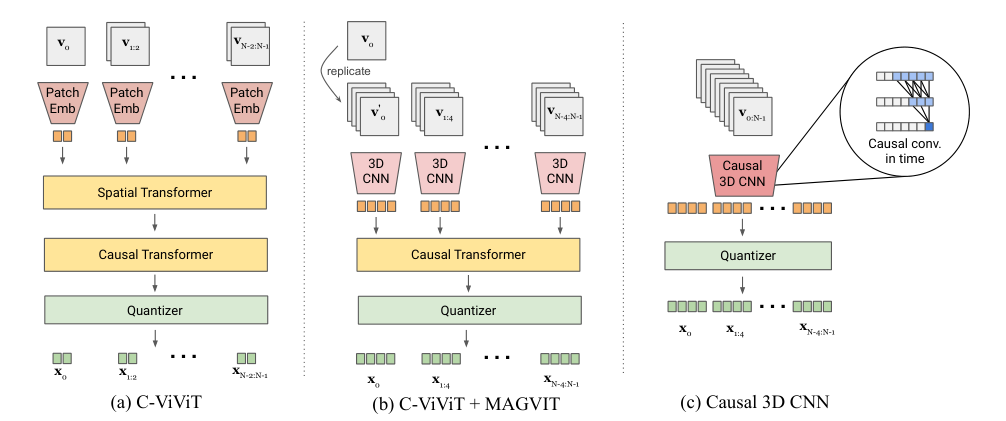
\includegraphics[keepaspectratio,alt={因果视频编码器的几种组织方式 （论文示意，来源：magvit-v2）}]{assets/seedance/figures/causal-tokenizer.png}}
\caption{因果视频编码器的几种组织方式 （论文示意，来源：magvit-v2）}
\end{figure}

图右的因果三维卷积，在时间上读取历史，在空间上仍读取邻域。这有助于理解视觉 tokenizer 怎样组织时空信息。但图中的离散量化器与这里连续 VAE 的概率潜变量不是同一种设计，借用结构示意时不能把两者直接替换。

保留首帧也意味着，有限帧数下的压缩率需要精确计算。以\textbf{元素数量}为单位，压缩后的元素与原像素元素之比是：

\[
r_F=\frac{48\left(1+(F-1)/4\right)}{3F\cdot16^2}.
\]

当 \(F\) 很大时，它趋近于 \(1/64\)；121 帧时约为 \(1/62.45\)，单张图片则是 \(1/16\)。这个比值没有考虑数据类型：原始像素可能是 uint8，潜变量可能是 BF16，不能直接把元素比当成显存字节比或视频文件压缩率。

\section{因果性来自输入索引}\label{seedance-m01-ux56e0ux679cux6027ux6765ux81eaux8f93ux5165ux7d22ux5f15}

再看“因果”在卷积里具体是什么意思。普通三维卷积的时间窗口可能覆盖前后帧；若要当前输出不读未来，就只能在时间轴左侧补齐。接着把 padding 和 stride 写进索引，才能检查这个说法是否真的成立。

设时间卷积核大小为 \(k_t\)，膨胀率为 \(\delta\)，步长为 \(s\)，左侧 padding 为：

\[
p=\delta(k_t-1).
\]

输出位置 \(j\) 读取的输入时间索引为：

\[
js-p+i\delta\le js,\qquad 0\le i<k_t.
\]

最大索引不超过 \(js\)，所以该输出没有读取未来。当核大小为 3、膨胀率为 1 时，序列 \codepath{[a,b,c,d]} 左补两个零，四个卷积窗口依次为 \codepath{[0,0,a]}、\codepath{[0,a,b]}、\codepath{[a,b,c]}、\codepath{[b,c,d]}。

PyTorch 对 \codepath{B,C,T,H,W} 张量的 padding 从最后一个维度开始填写：

\begin{verbatim}
# Conv3d 内部 padding 设为 0，空间 padding 另行计算。
x = F.pad(x, (pad_w, pad_w, pad_h, pad_h,
              dilation_t * (kernel_t - 1), 0))
y = conv(x)
\end{verbatim}

对应的时间输出长度是：

\[
F_{\mathrm{out}}=\left\lfloor\frac{F-1}{s}\right\rfloor+1.
\]

从长度式可以看到，步长设成 4，并不意味着所有输入帧数都可直接除以 4。首帧怎样处理，多出的帧怎样补或裁，最后解码怎样还原，必须是同一套约定。否则张量虽然能够接上，时间位置已经错了。

\section{整个网络怎样保持因果}\label{seedance-m01-ux6574ux4e2aux7f51ux7edcux600eux6837ux4fddux6301ux56e0ux679c}

不过，卷积这一层不读未来，是否就证明整个编码器因果了？还没有。若归一化同时统计整段时间的均值和方差，未来帧仍会改变前面的输出；跨时间注意力、重采样和特征缓存也可能带来同样的依赖。因此要沿完整计算图检查，不能停在一个卷积类上。

解码器还要处理时间展开。一个常见设计将 \(1+t\) 个潜时间位置展开为 \(1+st\) 帧；如果直接做普通 \(s\) 倍上采样，会得到 \(s+st\) 帧，需要配合首帧约定处理多出的 \(s-1\) 帧。采用 depth-to-space、插值加卷积或转置卷积时，长度和时间对齐规则各不相同，不能用统一的``裁掉尾部若干帧''替代依赖分析。

分块时问题还会再出现一次。每块若都重新补零，就相当于把每个块首当成视频起点，块边界自然可能接不上。所以除了历史特征，还得保留 stride 的采样相位：下一块从什么位置继续采样，也属于连续编码的定义。

\section{训练损失各自负责什么}\label{seedance-m01-ux8badux7ec3ux635fux5931ux5404ux81eaux8d1fux8d23ux4ec0ux4e48}

表示和长度确定后，才看这个压缩器怎样训练。一个常见写法是把重建、感知、分布约束和对抗项放在一起：

\[
\mathcal{L}=\lambda_1\lVert x-\hat{x}\rVert_1
+\lambda_p\mathcal{L}_{\mathrm{LPIPS}}
+\beta D_{\mathrm{KL}}\left(q(z\mid x)\Vert\mathcal{N}(0,I)\right)
+\lambda_a\mathcal{L}_{\mathrm{adv}}.
\]

其中 L1 看像素重建，LPIPS 看感知特征，KL 约束后验分布，判别器再提供纹理和运动监督。各项关心的量并不相同，所以权重、求和或平均的方式，以及判别器何时开始训练，都会改变优化。KL 太强可能损失细节，对抗项过早介入又可能不稳定，不能只看目标函数里有没有写齐这些名字。

最后可以反过来检查：真实视频经过编码和解码，细字、手部、快速运动与切镜还剩下多少？再扰动未来帧，看过去输出是否变化；比较整段与分块结果，看缓存是否接对。这些重建问题若还没有解决，就应先回到压缩器，而不是把丢失的细节都归因于生成主干。

\section{从极简代码到真实实现}\label{seedance-m01-ux4eceux6781ux7b80ux4ee3ux7801ux5230ux771fux5b9eux5b9eux73b0}

卷积的核心可以压缩成两步。设输入为 \codepath{B,C,T,H,W}，卷积内部不再自动补齐：

\begin{verbatim}
left = dilation_t * (kernel_t - 1)
x = F.pad(x, (pad_w, pad_w, pad_h, pad_h, left, 0))
y = conv3d(x)
\end{verbatim}

左侧 padding 决定时间依赖，空间 padding 负责尺寸。完整教学类见 \hyperref[code-causal-conv]{causal\_conv.py}；真实 VAE 的上下采样、归一化与特征缓存可直接读 \href{https://github.com/Wan-Video/Wan2.1/blob/9737cba9c1c3c4d04b33fcad41c111989865d315/wan/modules/vae.py}{Wan VAE}。

\chapter{文本与声音：条件特征和音频表示}
\label{seedance-encoders}

视频 VAE 已经给出了画面表示。总图输入侧还有文字与声音，
它们并非先变成视频像素再进入主干。下面继续按各自的输入、编码结果和用途来写。
具体规格沿用\hyperref[seedance-m05]{联合音视频章节}与\hyperref[seedance-m21]{模块接口}登记的
LTX-2 原系列，本文没有据此认定 Seedance 使用相同组件。

\section{文本编码器与主干投影分别做什么}
先取提示词的 token 序列 $w_{1:L}$，经配套文本编码器 $T$，得到
\[
H_c=T(w_{1:L})\in\mathbb R^{B\times L\times d_c}.
\]
这里特征宽度是文本编码器的输出宽度，并不要求等于视频流或声音流的隐藏宽度。
连接器与投影把它变成主干能够读取的条件，随后在相应文本 attention 中生成 K/V，
视觉或音频状态生成 Q。若使用联合多模态自注意力，文本也可以产生自己的 Q；
因此两种连接方式应按实际基座区分，不能只凭“文本条件”猜接口。

本文公开替代基座保留 Gemma 文本组件与配套连接器。冻结文本模型，
表示 $T$ 的参数不更新；新投影或参考实体汇聚是否更新，仍由各自参数组决定。
这两件事若混在一起，就容易把可学习支路误写成整个冻结条件。

另一个问题是角色词怎样对应参考图。正文 caption 可以继续走原生文本路径，
实体描述则先在原始 token 序列定位，汇聚后放入独立实体记忆，
与相应图像附同一个主体槽和 role。
连接器可能重组序列、插入 register，因此字符跨度不能直接当作连接器后的 token 索引。
具体绑定在\hyperref[seedance-m22]{参考身份与时间路由}中展开。

\section{声音的采样率与潜时间率}
声音首先是波形 $x^a[n]$，物理时间由 $\tau=n/f_s$ 给出。
codec 再将一段波形或配套声学表示映射到潜变量，潜时间位置有自己的速率。
两个速率分别描述原始采样与潜表示，不能把每秒样本数当成主干的 token 数。

LTX-2 原系列的接口例子中，音频输入使用 16kHz mel 表示，
codec 可保留 $B\times8\times T_a\times16$ 的布局。
进入主干前，将每个时间位置的两个特征轴整理为 $8\times16=128$ 维，
约每秒 25 个时间位置，再由输出端 vocoder 得到 24kHz 立体声。
这是一套配套输入输出约定，不表示任意 16kHz 编码器都能接相同解码器。

对时长 $D$，可以先估 $T_a\approx25D$，但实际还要遵守具体编码器的边界与长度规则。
每个潜 token 保存其覆盖区间，再与视频 VAE 的时间网格对齐。
视频帧、视频 latent、音频采样、音频 latent 的下标都不同，
跨模态 attention 应比较物理时间，而不是直接比较下标差。

\section{同一段声音在不同任务里是什么变量}
设编码结果为 $z_0^a=E_a(x^a)$。它可以有不同用途。
联合生成时，声音是未知目标，构造 $z_t^a$ 并回归相应速度；
音色参考时，它被汇聚成条件记忆，目标台词另行给定；
保留原音轨时，它是干净条件，采样器不再更新音频 latent，交付时复用原波形。

所以一个“音频已提供”的布尔变量还不够。
是否存在音轨、是否计算声音隐藏状态、是否更新声音目标、是否计算音频 loss，
分别控制不同路径。缺音轨没有目标，真实静音却仍有监督；
保持声音不更新，也不要求声音流停止给视频提供条件。
这些状态在\hyperref[seedance-m23]{音画编辑保持}中会逐项对应。

最后，声音隐藏状态可能读取当前视频。输入音轨固定以后，codec 特征可复用，
深层 Transformer 声音状态仍可能逐步变化。因此缓存结论要沿计算图继续追到依赖，
不能只停在源音频文件没有改变这一层。

% Imported from algorithms/reference-conditioning/README.md
\chapter{多模态参考控制}\label{seedance-m07}
\moduleinfo{M07}{基础方法与机制解释}{\hyperref[src-phantom]{\texttt{phantom}}、\hyperref[src-long-context-tuning]{\texttt{long-context-tuning}}、\hyperref[src-vincie]{\texttt{vincie}}、\hyperref[src-vincie-next]{\texttt{vincie-next}}、\hyperref[src-wan-2.1]{\texttt{wan-2.1}}、\hyperref[src-phantom-code]{\texttt{phantom-code}}}

表示已有以后，再沿总图的参考支路看：素材怎样成为可读取条件，目标主干怎样使用它。

把一张图作为参考，究竟是在参考什么？可能是人物身份，也可能只是衣服、构图或风格；动作视频还可能只负责相机运动。先把这个条件含义说清楚，再讨论编码。否则将素材全部拼接，连模型应该保留哪一部分都还没有定义。

例如人物 A 的脸来自图片，运动来自视频，音色来自音频。三者对目标的约束不同，绑定也要分别保留。若只传内容而不传用途，动作参考中的服装和背景、声音参考中的音乐，都可能一起进入结果。

\section{低层细节与高层语义各有什么用}\label{seedance-m07-ux4f4eux5c42ux7ec6ux8282ux4e0eux9ad8ux5c42ux8bedux4e49ux5404ux6709ux4ec0ux4e48ux7528}

对一张参考图，可以同时保留两类表示。VAE 潜变量保存纹理、颜色和局部结构，图像语义编码器再提供主体类别、外观概念及较抽象的身份信息。下面把它们写成两条条件路径：

\begin{figure}
\centering
\pandocbounded{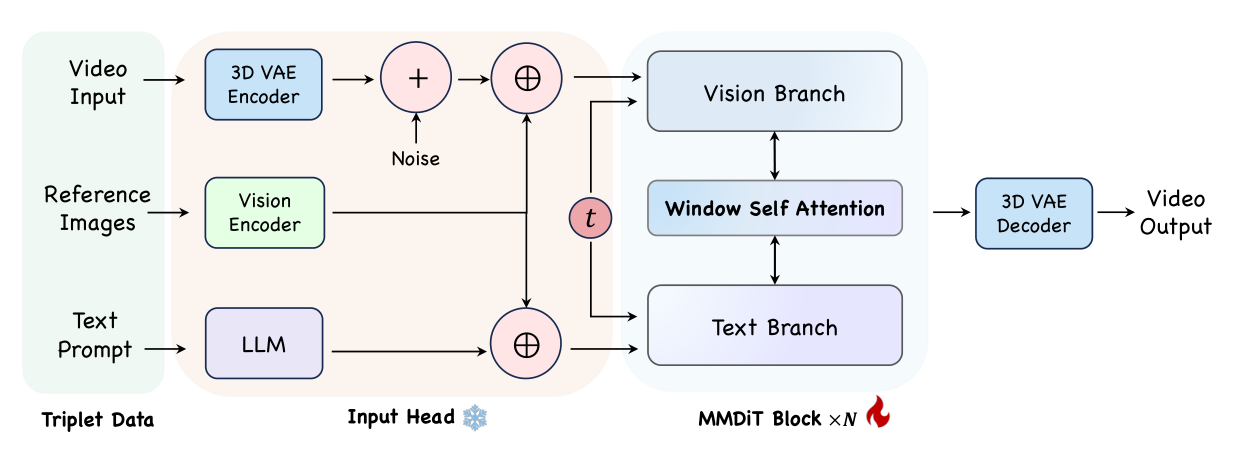
\includegraphics[keepaspectratio,alt={参考图细节与语义分别进入生成模型 （论文示意，来源：phantom）}]{assets/seedance/figures/subject-reference.png}}
\caption{参考图细节与语义分别进入生成模型 （论文示意，来源：phantom）}
\end{figure}

两条路径并不是越强越好。细节过强时，模型可能连姿态和背景都复制，视角、动作难以变化；语义过强时，又可能只剩“穿蓝衣的人”，具体长相和纹理丢掉了。因此可用条件 dropout、多视角配对和动作对照，检查每条路径到底保留了什么。

在窗口注意力中，还可以让参考信息进入多个窗口，使局部视频 token 都有机会读取主体信息。输入数量可变不代表开销不变，参考如何重复、压缩和聚合都需要明确。

\section{素材绑定应成为显式数据}\label{seedance-m07-ux7d20ux6750ux7ed1ux5b9aux5e94ux6210ux4e3aux663eux5f0fux6570ux636e}

每份素材至少记录 \codepath{asset_id}、\codepath{modality}、\codepath{role}、\codepath{subject_id}、\codepath{shot_ids}、\codepath{time_range} 和 \codepath{priority}。role 可以区分身份、外观、动作、相机、布局、风格与音色。

有了绑定，冲突才有地方处理。比如图片指定红外套，动作视频中的人却穿蓝外套：若视频只负责动作，它的服装信息就不应与图片争权重；若要求综合，先规定哪项优先。否则同一目标同时收到互斥条件，结果很难解释。

白模也属于参考条件。它可以先渲染为二维帧序列，或者额外提供 depth、normal、pose 和 camera 参数；不必天然使用原生 mesh encoder。显式结构条件通常更容易定位几何约束，但需要同步的训练数据和坐标定义。

\section{怎样在已有基座上增加参考能力}\label{seedance-m07-ux600eux6837ux5728ux5df2ux6709ux57faux5ea7ux4e0aux589eux52a0ux53c2ux8003ux80fdux529b}

若在现有基座上逐步加功能，可以先保留原 VAE、patch 与文本接口，只增一条参考读取路径。令目标视频给 query，参考给 key/value，门控控制新增残差，得到：

\[
\Delta h_v=\operatorname{Attn}(Q_v,K_r,V_r),
\qquad h'_v=h_v+g\Delta h_v.
\]

这一步的计算含义比较直接：每个视频位置问一个问题，参考记忆提供可以读取的内容，最后把读到的增量加回视频状态。是否使用某份参考，再由它与镜头、角色及时间的绑定来限制。这样参考怎样进入主干，就不再只是一句“加入参考条件”。

参考图先经过编码、投影与定额池化，得到 \codepath{B,R,d_ref} 的参考记忆。role、subject 和时间信息随 token 一起进入；视频 query 通过绑定 mask 读取适用的参考。

这个mask只能使用推理时真正可获得的信息：镜头允许的主体集合、布局、源视频跟踪或预测区域。纯噪声目标的空间query没有已知subject ID；无空间归属时先做镜头级粗筛，通过主体embedding和训练学习对应，不能假设一个标签已经解决多人空间绑定。

初始化也要沿计算图看。门控 \(g\) 从零开始，新投影正常作小方差初始化，先让支路能够在不扰动主干的情况下接入；若 gate 与整个支路同时全零，起始梯度可能被相互挡住。先训练参考支路，再用对照判断是否需要主干 LoRA 或有限解冻。

这里讨论的是独立 adapter。MMDiT 的窗口动态注入有自己的连接方式，不能把两种实现都叫“参考模块”就混用。应先看基座原本接收什么，再看手里的训练数据能监督哪一种关系。

\section{文件数量与 token 预算是两种容量}\label{seedance-m07-ux6587ux4ef6ux6570ux91cfux4e0e-token-ux9884ux7b97ux662fux4e24ux79cdux5bb9ux91cf}

假设视频有 \(N_v\) 个 token，参考编码后有 \(R\) 个 token。直接把参考拼进完整自注意力，新增连接规模约为：

\[
(N_v+R)^2-N_v^2=2N_vR+R^2.
\]

独立交叉注意力可以避免一部分不必要的参考内部交互，但仍有约 \(N_vR\) 的连接。几十个文件经过编码，可能变成远超几十个 token 的条件序列。

因此可以按镜头检索有效参考，再按优先级分配预算。例如先试总计 1024 个参考 token，比较它与更高预算的质量差异。这个数字只是试验起点，不能保证足以表示大量人物、精细 logo 和音色。

压成较少 token 后，细小部件也可能一起丢失。因此还要保存实际读取了哪些素材、怎样裁剪、保留多少 token，以及哪些被截断。用户提供了参考，与模型实际使用了参考，在这里仍是两个不同事实。

\section{参考训练数据怎样避免复制}\label{seedance-m07-ux53c2ux8003ux8badux7ec3ux6570ux636eux600eux6837ux907fux514dux590dux5236}

数据配对同样影响模型学到什么。从目标视频截一帧作参考，背景和姿态也高度相同，复制就可能把损失降下来。换成跨片段的同主体配对，才更接近保持身份、改变动作与环境的目标。不过相似 embedding 不能直接证明同一主体，错配会污染身份监督。

评测应同时改变参考数、主体数、背景、动作幅度和参考冲突程度，分别检查身份、服装、动作、相机和背景泄漏。先证明两到四份参考比最佳单参考更有帮助，再扩大数量，才能分清模型真正使用了多参考，还是接口仅仅接受了更多文件。

\section{从极简代码到真实实现}\label{seedance-m07-ux4eceux6781ux7b80ux4ee3ux7801ux5230ux771fux5b9eux5b9eux73b0}

参考支路的最小逻辑，是视频生成 query、参考生成 key/value，再按绑定 mask 限制读取：

\begin{verbatim}
q = video_projection(video)
k, v = reference_key(reference), reference_value(reference)
delta = attention(q, k, v, allowed_reference_mask)
output = video + gate * delta
\end{verbatim}

\hyperref[code-reference-adapter]{reference\_adapter.py} 保留了零门控和布尔绑定，假设每个 query 至少有一个有效参考。真实参考编码与采样看 \href{https://github.com/Phantom-video/Phantom/blob/bd84b602dcc949e23c89cbbf266b6f5975f2f025/phantom_wan/subject2video.py}{Phantom-Wan subject2video}，主干注入看 \href{https://github.com/Phantom-video/Phantom/blob/bd84b602dcc949e23c89cbbf266b6f5975f2f025/phantom_wan/modules/model.py}{Phantom-Wan model}。该固定版提供推理，训练代码仍未发布，不能把示例支路当成其训练复现。

% Imported from topics/video-generation/seedance-2.5/reference-timeline.md
\chapter{多参考绑定与时间控制}\label{seedance-m16}
\moduleinfo{M16}{候选设计与工程选型；组合效果待验证}{\hyperref[src-alchemint]{\texttt{alchemint}}、\hyperref[src-phantom]{\texttt{phantom}}、\hyperref[src-ltx-2]{\texttt{ltx-2}}、\hyperref[src-vace]{\texttt{vace}}}

上一章给出参考路径，这里继续展开参考内部的主体归属和时间条件。

多参考继续往下看，文件数量只是表面。两张图可能是同一人的不同角度，也可能是两个相似的人；动作视频里有背景，但目标只需要动作；人物还可能只在第十到十五秒出现。于是参考内容之外，还要同时给出归属和时间，模型才知道每项信息应该用到哪里。

下面以联合音视频主干写一套候选接口，把主体参考和时间控制接起来。参数与预算用于明确计算关系，尚未通过训练验证，不把它们当成已经测得的配置。

\section{一份参考先拆成三个对象}\label{seedance-m16-ux4e00ux4efdux53c2ux8003ux5148ux62c6ux6210ux4e09ux4e2aux5bf9ux8c61}

第一层是原始资产，例如图片、视频或音频。第二层是主体，例如 \codepath{actor_a}、\codepath{car_b}、\codepath{speaker_a}。第三层是绑定规则，说明资产为哪个主体、哪个镜头、哪段时间提供哪类信息。

\begin{verbatim}
{
  "asset_id": "portrait_a_front",
  "subject_id": "actor_a",
  "role": "identity",
  "shot_ids": ["shot_2"],
  "active_intervals_seconds": [[10, 15]],
  "priority": 1
}
\end{verbatim}

\codepath{asset_id} 用来区分文件，\codepath{subject_id} 用来合并同一人的多张视图，\codepath{role} 用来限制应当继承的属性。声音与人物之间另用 speaker-to-subject 映射，不能假设第一段音频必然属于第一张图片。

时间也不能只保留首次和末次出现。人物出现、离开、又回来，中间有一段明确缺席；若直接取两端，就会把缺席也填成出场。因此这里保留区间列表。

\section{描述词与图像为什么需要相同绑定}\label{seedance-m16-ux63cfux8ff0ux8bcdux4e0eux56feux50cfux4e3aux4ec0ux4e48ux9700ux8981ux76f8ux540cux7ed1ux5b9a}

文本绑定的原因可以从两个男人的例子看出来。只写“男人转身”，没有说明是哪一个；若角色描述和对应图片使用同一个索引或角色表示，两个条件就有了共同指向，身份串用的问题才有可监督的对象。

\begin{figure}
\centering
\pandocbounded{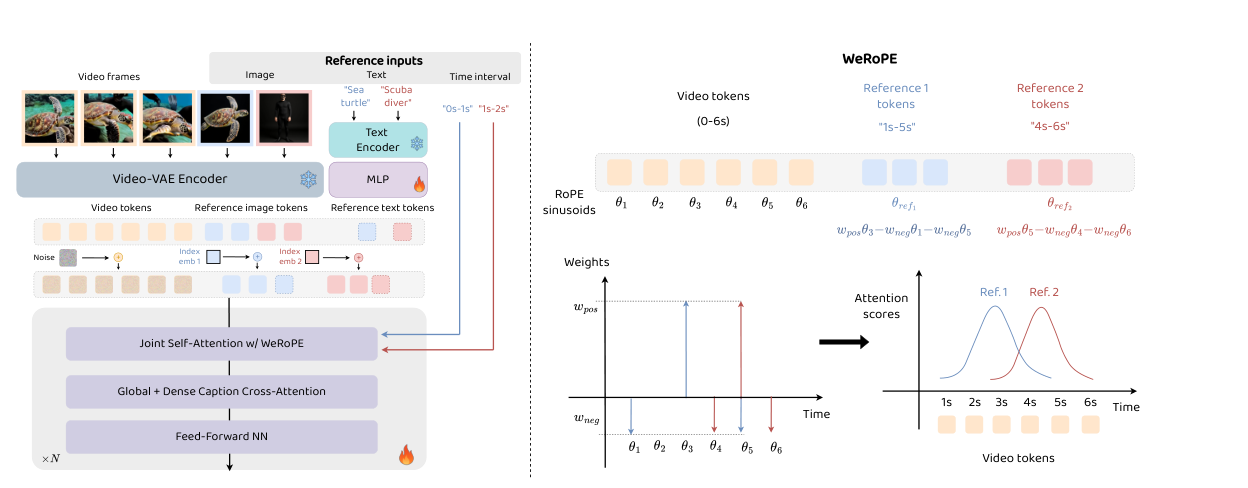
\includegraphics[keepaspectratio,alt={参考图、主体描述与时间区间共同进入模型 （论文示意，来源：alchemint）}]{assets/seedance/figures/timed-reference.png}}
\caption{参考图、主体描述与时间区间共同进入模型 （论文示意，来源：alchemint）}
\end{figure}

图里因此不只放参考图，还放实体词和区间。描述词与图像由同一索引关联，时间再决定它们何时与视频 token 交互。仅在长提示里重复角色名字，并没有显式提供这种内容、归属与时间的对应。

但归属 embedding 仍只是标签。标签告诉模型这些特征属于同一人，脸和服装长什么样还得由图像提供。若素材没有相应外观信息，增加角色标签也不能把它补回来。

\section{三种模态分别怎样编码}\label{seedance-m16-ux4e09ux79cdux6a21ux6001ux5206ux522bux600eux6837ux7f16ux7801}

{\def\LTcaptype{table} % do not increment counter
\small\setlength{\tabcolsep}{3pt}\renewcommand{\arraystretch}{1.18}
\begin{longtable}[]{@{}
  >{\raggedright\arraybackslash}p{(\linewidth - 4\tabcolsep) * \real{0.1900}}
  >{\raggedright\arraybackslash}p{(\linewidth - 4\tabcolsep) * \real{0.3900}}
  >{\raggedright\arraybackslash}p{(\linewidth - 4\tabcolsep) * \real{0.4200}}@{}}
\toprule\noalign{}
\begin{minipage}[b]{\linewidth}\raggedright
输入
\end{minipage} & \begin{minipage}[b]{\linewidth}\raggedright
内容路径
\end{minipage} & \begin{minipage}[b]{\linewidth}\raggedright
需要分开的角色信息
\end{minipage} \\
\midrule\noalign{}
\endhead
\bottomrule\noalign{}
\endlastfoot
图片 & 与目标视频相同的 VAE、空间投影、主体 crop & 身份、服装、场景、风格 \\
视频 & VAE 时空特征；额外提取 pose、flow、相机轨迹 & 动作与相机不能默认继承人物身份 \\
音频 & 同一音频 VAE 的时序特征、说话人分段与文字转录 & 音色、节奏、对白内容、音乐 \\
\end{longtable}
}

图片与视频先使用同一个视觉潜空间，避免又引入一套没有对齐的像素表示。不过每份素材要独立编码：不连续视频若先在像素时间轴拼接，因果 VAE 会把前一份素材当作后一份的历史，边界关系已经变了。

只借动作时，可以优先送姿态、光流和相机条件，关闭不需要的外观 token。音频也一样，一句参考语音可能只提供音色，不是要求输出这句台词。同说话人跨文本配对监督音色，时间对齐文字与波形监督逐字对白，两者的数据定义不同。

音色和风格可以压成摘要，精确对白、节拍或已有配乐则不能只靠32个摘要token承载。需要保持原声音和时序时，使用对齐到目标媒体时钟的完整干净音频条件，输出复用原波形；对应约25Hz的条件序列单独计入计算预算。这样要与``只借音色、生成新台词''的任务分开训练。

\section{固定预算怎样保留细节}\label{seedance-m16-ux56faux5b9aux9884ux7b97ux600eux6837ux4fddux7559ux7ec6ux8282}

候选起点为每图 32 个摘要 token、每视频 64 个、每音频 32 个。30 图和 10 视频共 1600 个视觉参考 token，10 音频共 320 个音频参考 token，分别位于 2048 与 512 的预算以内。

这些是\textbf{压缩后的条件预算}，不是原始 VAE 序列长度，也不是已证明充分的容量。先用少量可学习 query 对每份素材独立汇聚：

\[
R_j=\operatorname{Attn}(Q_j^{\mathrm{pool}},K_j^{\mathrm{asset}},V_j^{\mathrm{asset}}).
\]

压缩之前先保留局部结构：图片有 crop 坐标，视频有动作阶段，音频有时间段与 speaker，再加 role、subject 和位置。若先把所有素材平均成一个向量，后面就很难再恢复哪一部分来自哪个人。

读取也按镜头进行。细 logo、纹理或音色在压缩中消失时，应先调整相应主体的预算，或用确定性合成处理交付；继续增加无关镜头的素材，不能恢复已经丢掉的信息。

\section{时间控制放在哪里}\label{seedance-m16-ux65f6ux95f4ux63a7ux5236ux653eux5728ux54eaux91cc}

时间控制可以放进参考位置，也可以放进 cross-attention 的偏置。加权 RoPE 尝试让一个参考在整个区间持续可读，而不只编码区间中点，因此有机会区分长短区间。这里仍是学习型偏置，尚不能从注意力分数直接推出人物一定按时出场。

为降低首版迁移风险，这套候选方案先保留主干原 RoPE，只在新增参考支路增加显式时间门：

\[
g_j(\tau)=\sum_k
\sigma\!\left(\frac{\tau-a_{jk}}{\delta}\right)
\sigma\!\left(\frac{b_{jk}-\tau}{\delta}\right).
\]

区间为 \([a_{jk},b_{jk})\)，\(\delta\) 控制边界过渡。实际将重叠区间合并，并把 \(g_j\) 限制到 \([0,1]\)。对应 attention bias 为：

\[
B_{ij}=\log\bigl(\varepsilon+(1-\varepsilon)g_j(\tau_i)\bigr).
\]

因为 attention 在 softmax 前加上 \(B_{ij}\)，相当于在归一化前将该参考位置的指数权重乘以 \(\varepsilon+(1-\varepsilon)g_j(\tau_i)\)。所以这个时间门是在改变读取权重；它没有直接改写目标人物是否存在，后面的正负时间监督仍然需要。

角色或镜头不相容时，可以把连接直接屏蔽；时间边缘先用软门，留出进入、离开与运动模糊的过渡。还要保留一个始终可读的 null token，否则某行参考全部不可见，softmax 本身就没有定义。

空间query并不天然知道自己属于哪个主体。没有布局、源跟踪或可靠预测区域时，只按镜头允许的主体集合做粗筛，靠共享主体embedding与训练学习对应；有可靠区域时才加入空间约束。训练中若使用真值区域，推理也必须提供相同类型的条件，或在训练时混入预测误差，不能借用目标真值暗中完成绑定。

\section{不能把``看不到参考''当成``角色一定不出现''}\label{seedance-m16-ux4e0dux80fdux628aux770bux4e0dux5230ux53c2ux8003ux5f53ux6210ux89d2ux8272ux4e00ux5b9aux4e0dux51faux73b0}

注意力控制住了参考，是否也就控制住人物出场？还没有。文本或历史仍可能让主干在区间外生成人物。因此训练必须同时有区间内出现、区间外缺席，以及多人重叠的样本，让“什么时候不出现”也进入监督。

可从实体词、检测与分割跟踪提取可见区间，再选与目标相隔较远的主体视图，减少复制。不过没检测到，不一定就是离场，也可能被遮挡，所以标签要保存可见性置信度，不能把所有漏检写成角色不存在。

验收分别统计区间内身份、区间外误出现、边界误差、多人串用、动作跟随和背景泄漏。两图两个角色、相同中点不同区间长度、间断出场和同时出场，都是必须保留的对照。

\section{极简代码与工程入口}\label{seedance-m16-ux6781ux7b80ux4ee3ux7801ux4e0eux5de5ux7a0bux5165ux53e3}

单区间时间 bias 的计算见 \hyperref[code-reference-timing]{reference\_timing.py}，多区间需先按主体合并。参考支路的布尔可读mask见 \hyperref[code-reference-adapter]{reference\_adapter.py}；将时间bias与归属mask合成、添加null token由调用者完成。这些代码只说明机制，未执行。

真实主体参考可从 \href{https://github.com/Phantom-video/Phantom}{Phantom-Wan} 阅读；时间控制方法的 \href{https://snap-research.github.io/Video-AlcheMinT/}{AlcheMinT 项目} 提供论文与展示。本方案采用显式时间门作为首版设计，不将它称为 WeRoPE 原实现，也不声称这些方法已被用于 Seedance 2.5。

% Imported from topics/video-generation/seedance-2.5/reference-binding-spec.md
\chapter{主体槽、参考冲突与细节预算}\label{seedance-m22}
\moduleinfo{M22}{候选设计与工程选型；组合效果待验证}{\hyperref[src-alchemint]{\texttt{alchemint}}、\hyperref[src-phantom]{\texttt{phantom}}、\hyperref[src-ltx-2]{\texttt{ltx-2}}、\hyperref[src-ltx-original-code]{\texttt{ltx-original-code}}、\hyperref[src-vace]{\texttt{vace}}}

参考的内容、归属与时间已经定义，接着把素材身份、池化预算和读取规则落实到同一接口。

再看一个完整参考输入：角色 A 有六张脸和服装图，角色 B 有两张，商品图约束外观，动作来自一段视频，声音又来自两段语音。文件都能编码，并不说明生成 A 时会读到 A 的脸，或动作视频中的衣服不会一并复制。还需要把这些关系表示出来。

所以本节继续固定素材、主体、属性和时间之间的对应，再讨论冲突与预算。以下仍是联合音视频主干上的候选规则，宽度和压缩容量尚未经模型验证。

\section{主体槽是一次任务中的关系}\label{seedance-m22-ux4e3bux4f53ux69fdux662fux4e00ux6b21ux4efbux52a1ux4e2dux7684ux5173ux7cfb}

素材身份用内容哈希和 \codepath{asset_id}；人物或商品用稳定业务ID；模型则使用场景局部主体槽，例如A、B、product。业务ID用于检索，局部槽用于表示这一次请求中的对应关系。

局部槽号的作用是本次请求中的对应，并不是永久身份。训练时可同时置换 A/B 槽，以及所有相关文本、图像、声音与区域标签，迫使模型读关系而不是记住第 0 槽总是主角。人物实际长相仍由素材给出。

\begin{verbatim}
{
  "asset_id": "a_coat_front",
  "subject_slot": "A",
  "roles": ["clothing"],
  "shot_ids": ["s2"],
  "active_intervals_seconds": [[8, 12], [15, 18]],
  "priority": 2,
  "confidence": 0.95
}
\end{verbatim}

同一图片需要同时提供脸和服装时，保留一个资产、建立两个属性视图；不复制成两个互相无关的主体。音频另保留speaker-to-subject映射，群体环境声没有人物槽。

\section{实体词与视觉特征怎样共享绑定}\label{seedance-m22-ux5b9eux4f53ux8bcdux4e0eux89c6ux89c9ux7279ux5f81ux600eux6837ux5171ux4eabux7ed1ux5b9a}

实体文本先从冻结文本模型的原始 token 序列中定位描述范围，汇聚特征，再投影成 512 维记忆。与它对应的图像摘要使用相同主体槽和 role 表示，于是文字与视觉条件有了共同指向。

字符偏移还不能直接当作连接器后的 token 位置：连接器可能改变序列并添加 register。首版因此单独保存实体条件记忆，原 caption 仍沿原生文本路径，同时记录实体跨度和 tokenizer 版本，避免索引看似对齐，读到的却是另一段内容。

每个图像资产独立VAE编码，空间坐标与局部crop信息进入池化器；每段参考视频保留自己的时间轴，不与其它素材在像素时间维拼接。音色素材由音频codec独立编码，文字转录只用于区分声音内容与声音身份。

\section{先分配预算，再进行汇聚}\label{seedance-m22-ux5148ux5206ux914dux9884ux7b97ux518dux8fdbux884cux6c47ux805a}

候选共享记忆宽度512。视觉总预算2048，声音摘要预算512，null token单独增加一个位置；这些预算表示可读取记忆长度，不包含原始素材编码开销。

{\def\LTcaptype{table} % do not increment counter
\small\setlength{\tabcolsep}{3pt}\renewcommand{\arraystretch}{1.18}
\begin{longtable}[]{@{}
  >{\raggedright\arraybackslash}p{(\linewidth - 4\tabcolsep) * \real{0.1900}}
  >{\raggedleft\arraybackslash}p{(\linewidth - 4\tabcolsep) * \real{0.3900}}
  >{\raggedright\arraybackslash}p{(\linewidth - 4\tabcolsep) * \real{0.4200}}@{}}
\toprule\noalign{}
\begin{minipage}[b]{\linewidth}\raggedright
角色
\end{minipage} & \begin{minipage}[b]{\linewidth}\raggedleft
默认摘要数
\end{minipage} & \begin{minipage}[b]{\linewidth}\raggedright
额外保留什么
\end{minipage} \\
\midrule\noalign{}
\endhead
\bottomrule\noalign{}
\endlastfoot
人物/商品图片 & 32/图 & 主体crop、视角和关键细节crop \\
外观参考视频 & 64/段 & 分段时间、视角与可见性 \\
音色/声音风格 & 32/段 & speaker、干净语音段与文字内容标签 \\
仅动作/相机视频 & 不占身份摘要 & pose/flow/相机走结构路径，单独计费 \\
必须逐字/逐拍保留的音轨 & 不压成声音摘要 & 完整原生时序音频条件 \\
\end{longtable}
}

预算先满足本镜头必要主体，再按优先级和不确定性分配剩余量。不够时先去掉无关镜头、近重复视角和低质量素材，并登记裁减结果。否则唯一背面或唯一 speaker 参考被悄悄丢掉，后面再调强度也不能补回这份条件。

30图＋10外观视频按默认预算为1600视觉位置，10音频为320声音位置。两类都能放进预算，只证明输入可表示；没有证明小logo、多人身份和音色细节仍然充分。

池化前保留crop坐标、素材内时间和type信息。对细字、商标和精密结构，摘要容量不足时增加局部预算，或通过确定性图层交付；摘要token不能承诺恢复已经丢掉的像素信息。

\section{可读性由三层规则决定}\label{seedance-m22-ux53efux8bfbux6027ux7531ux4e09ux5c42ux89c4ux5219ux51b3ux5b9a}

对视频query \(i\) 与参考位置 \(j\)，先判定镜头和属性是否允许，再计算时间偏置：

\[
B_{ij}=\log\left(\varepsilon+(1-\varepsilon)g_j(\tau_i)\right)
+\log(\max(c_j,\varepsilon))+H_{ij}.
\]

\(c_j\in[0,1]\)是置信度；\(H_{ij}\)为兼容时0、不兼容时负无穷。时间函数 \(g_j\) 合并同主体的重叠区间，对多次出场分别计算软门，再限制到 \([0,1]\)。null位置始终有限且不施加置信度惩罚。

空间query没有已知主体槽，默认只做镜头级粗筛。用户布局、源视频跟踪或可靠预测区域存在时，可进一步限制空间归属；遮挡边界使用软区域，而不是强行把一个latent只分给一个人物。

多人混合音频的一个时间token也可能含两个speaker。声音支路按明确对白时间和说话人映射路由，重叠讲话使用集合或软权重；没有说话人时间信息时保留不确定性，不能由文件顺序猜声音归属。

\section{冲突如何进入任务编译}\label{seedance-m22-ux51b2ux7a81ux5982ux4f55ux8fdbux5165ux4efbux52a1ux7f16ux8bd1}

相似图像未必是冲突：同一人的两个视角可以互补；同一时刻又要求同一人穿两套互斥服装，才需要裁决。判断必须结合属性、时间与优先级，对全部图像简单平均没有表达这种区别。

{\def\LTcaptype{table} % do not increment counter
\small\setlength{\tabcolsep}{3pt}\renewcommand{\arraystretch}{1.18}
\begin{longtable}[]{@{}
  >{\raggedright\arraybackslash}p{(\linewidth - 2\tabcolsep) * \real{0.2200}}
  >{\raggedright\arraybackslash}p{(\linewidth - 2\tabcolsep) * \real{0.7800}}@{}}
\toprule\noalign{}
\begin{minipage}[b]{\linewidth}\raggedright
情况
\end{minipage} & \begin{minipage}[b]{\linewidth}\raggedright
首版处理
\end{minipage} \\
\midrule\noalign{}
\endhead
\bottomrule\noalign{}
\endlastfoot
同主体多视角 & 共用主体槽，保留视角标签 \\
同主体前后换衣 & 为服装属性分别设置区间，身份参考持续有效 \\
同一时段两套互斥服装 & 采用显式优先级；无优先级则返回规格冲突 \\
动作视频人物与身份参考不同 & 禁用其外观记忆，只传结构条件 \\
声音参考包含音乐/他人讲话 & 分段或分离后用；无法分离则降低置信度或回到后期音轨方案 \\
同一角色离场后返回 & 保留身份记忆，出场监督记录多个区间 \\
\end{longtable}
}

置信度表示我们是否确定这条信息，并不改变用户是否要求它成立。低置信但必需的条件，应回到输入修正，而不能被自动降权后当作已经满足。

\section{训练要教会什么}\label{seedance-m22-ux8badux7ec3ux8981ux6559ux4f1aux4ec0ux4e48}

参考正确但背景不同、参考服装不同、相似人物同时出现、人物暂时遮挡、角色真正离场、声色与台词不同，是不同的数据切片。只收集``人物一直在画面中央''的正例，不足以学习绑定。

保持目标不变时，可以同时置换槽号或素材顺序，也可以增加无关素材、去掉重复视角，检查模型是否仍遵守同一关系。但把 A 的参考换成 B，目标仍写 A，就已经改变条件与目标的匹配，不能继续当成同一条正确生成监督。

错误参考可用来训练冲突检测、绑定分类或偏好比较；生成分支则只作训练约定内的条件 dropout。这样模型学到的“忽略条件”才有明确原因，不会被矛盾样本反复强化。

\section{验收使用成组任务}\label{seedance-m22-ux9a8cux6536ux4f7fux7528ux6210ux7ec4ux4efbux52a1}

至少保留单主体新背景、两主体相似外观、多人重叠、换衣、间断出场、动作换身份、同音色新台词和文件数上限八类。每类分别看身份、动作、误出场、边界偏差、背景泄漏和声音归属，不能只报告总体美感。

几个对照可以直接检验关系是否真的被使用：文本不动只换参考，参考不动只换时间，所有槽同步置换，或者只打乱文件顺序。正确行为应随语义绑定变化，而不应依赖某个文件刚好排在第几位。

时间偏置的极简示例见 \hyperref[code-reference-timing]{reference\_timing.py}，候选读取见 \hyperref[code-gated-condition]{gated\_condition.py}。真实主体参考结构可读 \href{https://github.com/Phantom-video/Phantom}{Phantom}，它提供的实现和这里的摘要路由、音频绑定不是同一套完整工程。

% Imported from algorithms/video-editing/README.md
\chapter{视频局部编辑}\label{seedance-m08}
\moduleinfo{M08}{基础方法与机制解释}{\hyperref[src-seedance-1.0]{\texttt{seedance-1.0}}、\hyperref[src-vincie]{\texttt{vincie}}、\hyperref[src-vincie-next]{\texttt{vincie-next}}、\hyperref[src-seedance-2.5-release]{\texttt{seedance-2.5-release}}、\hyperref[src-vincie-code]{\texttt{vincie-code}}、\hyperref[src-ltx-code]{\texttt{ltx-code}}}

从参考支路转到源条件支路：编辑先定义变化与保持，再决定怎样编码和合成。

再把生成改成编辑。要求“第二到第四秒的外套变红，其它不动”，目标已经不只是输出一段相似视频，而是同时规定变化对象、时间与保持范围。若这些关系只留在一句提示里，模型即使改对衣服，也可能顺便改了人脸或背景。这里把这几个量分开写。

\section{时间指令怎样变成帧范围}\label{seedance-m08-ux65f6ux95f4ux6307ux4ee4ux600eux6837ux53d8ux6210ux5e27ux8303ux56f4}

先将指令对应到源视频版本、半开时间区间 \([2,4)\)、目标主体和服装区域。随后把不应变化的脸、姿态、背景和音轨也列出来。这样编辑的未知量与已知条件才各有范围。

固定 24 fps 且时间起点为零时，该区间包含帧号 48 到 95。可变帧率视频则应按真实时间戳选帧，不能只用时间乘平均 fps。还要约定第四秒以后是恢复原色，还是延续编辑后的外观；两者对应不同目标。

\section{为什么需要三种 mask}\label{seedance-m08-ux4e3aux4ec0ux4e48ux9700ux8981ux4e09ux79cd-mask}

不过，像素上画出的区域，进入 VAE 和 DiT 后还是同一组独立位置吗？一般不是。时间压缩、卷积感受野与 patch 会混合邻域信息，所以不能把一个像素 mask 不加区分地沿所有阶段使用。需要分别定义：

{\def\LTcaptype{table} % do not increment counter
\small\setlength{\tabcolsep}{3pt}\renewcommand{\arraystretch}{1.18}
\begin{longtable}[]{@{}
  >{\raggedright\arraybackslash}p{(\linewidth - 2\tabcolsep) * \real{0.2200}}
  >{\raggedright\arraybackslash}p{(\linewidth - 2\tabcolsep) * \real{0.7800}}@{}}
\toprule\noalign{}
\begin{minipage}[b]{\linewidth}\raggedright
mask
\end{minipage} & \begin{minipage}[b]{\linewidth}\raggedright
作用
\end{minipage} \\
\midrule\noalign{}
\endhead
\bottomrule\noalign{}
\endlastfoot
编辑 mask & 用户允许最终改变的区域与时间 \\
上下文 mask & 模型需要读取或重建的邻域 \\
损失 mask & 哪些位置具有有效监督 \\
\end{longtable}
}

因此，模型工作区可以向外扩一些，让它读取边界上下文，交付时再按约定只替换允许区域。若改光照本来就会影响外部阴影，则应先扩大允许变化范围；不能既要求全局物理一致，又禁止外部任何像素变化。

\section{生成式补全与像素保留怎样配合}\label{seedance-m08-ux751fux6210ux5f0fux8865ux5168ux4e0eux50cfux7d20ux4fddux7559ux600eux6837ux914dux5408}

一种做法是以源潜变量、mask 和指令为条件，重新生成工作区，较大语义变化容易表达，但外区也可能漂移、边界可能闪烁。另一种做法只生成局部，随后复用外面的源帧。两者的保持机制不同，下面先看后一种合成关系。

设 \(M\) 为最终编辑权重，合成结果为：

\[
x_{\mathrm{out}}=M\odot x_{\mathrm{generated}}+(1-M)\odot x_{\mathrm{source}}.
\]

这个式子中，\(M=0\) 的不编辑位置直接取源像素，因此不必再要求有损 VAE 无损重建外区。软 mask 可以处理过渡，但发丝、运动模糊、透明材质和前后遮挡仍需另外处理。音轨若要求严格保留，也应复用原采样，并检查混流后是否引入延迟。

\section{编辑监督从哪里来}\label{seedance-m08-ux7f16ux8f91ux76d1ux7763ux4eceux54eaux91ccux6765}

真实视频天然包含外观、姿态和物体状态的变化，可以用于挖掘编辑指令和变化区域。

\begin{figure}
\centering
\pandocbounded{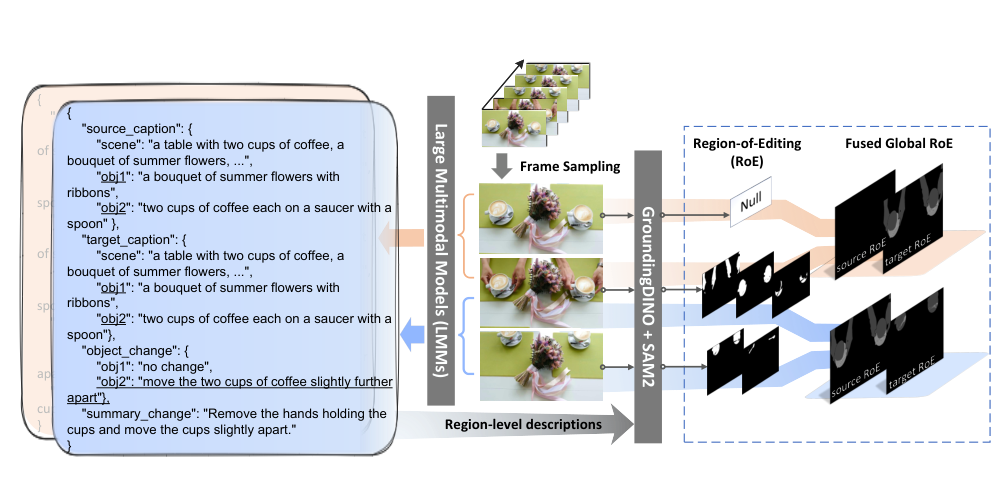
\includegraphics[keepaspectratio,alt={从视频变化构造编辑描述与区域 （论文示意，来源：vincie）}]{assets/seedance/figures/edit-data.png}}
\caption{从视频变化构造编辑描述与区域 （论文示意，来源：vincie）}
\end{figure}

看起来可以从相邻帧直接挖出很多“修改前后对”，但两帧之间可能不止一个因素变化。相机、遮挡、光照都在动，却只标“换衣服颜色”，训练就会把其它变化也学成这条指令的一部分。因此这种配对还不能当作精确单因素真值。

数据来源可以继续分开：受控三维重渲染提供精确几何与 mask；人工真实编辑对记录具体后期操作；视频变化挖掘则作为带置信度的弱监督，并作抽检。三类可以混合使用，但监督的确定程度不能混成一类。

\section{白模与绿幕分别控制什么}\label{seedance-m08-ux767dux6a21ux4e0eux7effux5e55ux5206ux522bux63a7ux5236ux4ec0ux4e48}

白模将布局、相机和运动轨迹先固定，再让生成模型补材质、风格与光照。若同时输出 depth、normal、pose 和相机参数，几何条件更明确；训练时必须保持它们与目标帧严格对齐。由单目视频估计的深度和相机存在误差，需要与精确渲染真值区分。

绿幕编辑先处理 alpha、绿溢色、发丝和运动模糊，再生成背景并做前景光色融合。若还希望衣服受风、头发运动和接触阴影随背景重新变化，任务已经超出单纯抠像，需要重新生成部分前景，并额外验证身份与动作保持。

\section{编辑是否成功，要拆开评价}\label{seedance-m08-ux7f16ux8f91ux662fux5426ux6210ux529fux8981ux62c6ux5f00ux8bc4ux4ef7}

编辑成功怎样看？先确认目标有没有变化，再看非目标有没有保持，接着看时间边界、闪烁、遮挡和音轨。只改颜色可以比较外区像素；改视角时像素本来就变了，应比较身份、语义和几何关系。评价也要随任务定义改变。

编辑并不以 KV 缓存为前提。先用完整重算得到正确结果，再优化哪些依赖可以复用；改动过去内容时，依赖它的后续状态要刷新。最终检查也应覆盖编辑区间前后的帧，不能只挑变化最明显的一张截图。

\section{从极简代码到真实实现}\label{seedance-m08-ux4eceux6781ux7b80ux4ee3ux7801ux5230ux771fux5b9eux5b9eux73b0}

最终保持源像素，只需要明确合成权重；模型内部的工作区和噪声覆盖则是另外两层逻辑：

\begin{verbatim}
selected = (frame_pts >= start) & (frame_pts < end)
output = alpha * generated + (1 - alpha) * source
\end{verbatim}

三种操作的极简代码见 \hyperref[code-local-edit]{local\_edit.py}。真实多轮图像编辑看 \href{https://github.com/ByteDance-Seed/VINCIE/blob/97cd2c5701e694dabcfea320c0cf59893d427fab/generate.py}{VINCIEGenerator}；视频和音视频条件流水线可从 \href{https://github.com/Lightricks/LTX-2/blob/daa6b16fc7f0f1628f2c9e36a303e3312b333cc6/packages/ltx-pipelines/README.md}{LTX pipelines} 选择。VINCIE 的图像编辑入口本身不是时间戳视频编辑器。

% Imported from topics/video-generation/seedance-2.5/editing-conditions.md
\chapter{源条件与统一编辑接口}\label{seedance-m17}
\moduleinfo{M17}{候选设计与工程选型；组合效果待验证}{\hyperref[src-vace]{\texttt{vace}}、\hyperref[src-videocof]{\texttt{videocof}}、\hyperref[src-vincie-next]{\texttt{vincie-next}}、\hyperref[src-ltx-2]{\texttt{ltx-2}}}

编辑的变化范围已经明确，这里把源内容、区域与目标分别写成主干可以接收的条件。

编辑再细看，会遇到连续三个未知量：指令中的对象是谁，哪一片区域需要变，这种变化怎样沿时间传播？若只送入源视频和一句指令，三者都藏在同一个隐含过程里，失败后难判断哪一步出了问题，数据也难以分别监督。

所以这里把用户给定条件、预测区域与生成目标分开，仍由共同视频主干处理。先写出这些对象的关系，再决定各自从哪条支路进入网络。

\section{用帧与 mask 表示不同任务}\label{seedance-m17-ux7528ux5e27ux4e0e-mask-ux8868ux793aux4e0dux540cux4efbux52a1}

设源条件为 \(F\)，编辑 mask 为 \(M\)，其中 \(M=1\) 表示允许重新生成。可将条件分成两路：

\[
F_c=F\odot M,\qquad F_k=F\odot(1-M).
\]

\(F_c\) 放待改变内容或控制信号，\(F_k\) 放必须保留的信息。分别编码后，再连同压缩到相同网格的 mask 进入条件支路：

\[
C_{\mathrm{edit}}=P\bigl[E_v(F_c);E_v(F_k);D(M)\bigr].
\]

源内容先拆成待变与保留两路，再各自编码，最后与对齐的 mask 拼接并投影。目标 noisy latent 另走原输入，因此条件表示和生成目标在这一步并没有混成同一个张量。这个区分也解释了为什么新增支路可以不改旧输入头。

分号表示通道拼接，\(D\) 表示保持对齐的 mask 变换。目标的带噪 latent 仍走原主干输入，新增条件支路在选定层提供残差信息，不直接改写旧 checkpoint 的输入通道。

\begin{figure}
\centering
\pandocbounded{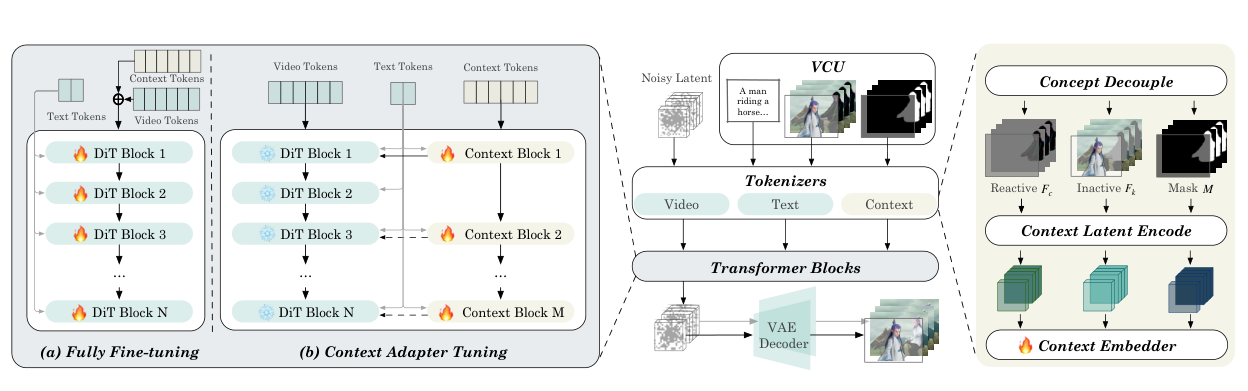
\includegraphics[keepaspectratio,alt={视觉条件的拆分、编码与主干残差连接 （论文示意，来源：vace）}]{assets/seedance/figures/unified-context.png}}
\caption{视觉条件的拆分、编码与主干残差连接 （论文示意，来源：vace）}
\end{figure}

这套表示可以覆盖几种任务：空条件和全生成 mask 对应文生视频；源帧与全生成 mask 对应重绘；源帧与局部 mask 对应局部编辑；历史帧可作为续写条件。它们使用相近接口，却仍需要各自的训练样本，表示统一不能推出任务能力自然齐全。

\section{时间和空间需要同时定义}\label{seedance-m17-ux65f6ux95f4ux548cux7a7aux95f4ux9700ux8981ux540cux65f6ux5b9aux4e49}

用户要求``第二到第四秒更换角色 A 的外套''时，最终编辑范围可写为：

\[
M(\tau,y,x)=M_{\mathrm{coat},A}(\tau,y,x)
\cdot\mathbf{1}_{[2,4)}(\tau).
\]

模型要读取边界上下文，因此工作区按 VAE 和 patch 感受野适当扩张；最终交付的替换范围仍由用户要求决定。若还要让阴影、光照或遮挡一起变化，就继续说明这些影响是否被允许，不能只靠一个对象框代表所有约束。

源视频、参考图、区域条件与目标各自编码，避免不连续素材在因果 VAE 中互相影响。loss mask、条件 mask 与最终 alpha 也分开保存，它们虽然来自同一个任务范围，承担的计算含义却不同。

\section{用户不提供 mask 时，先定位再编辑}\label{seedance-m17-ux7528ux6237ux4e0dux63d0ux4f9b-mask-ux65f6ux5148ux5b9aux4f4dux518dux7f16ux8f91}

例如指令只说“删除右边穿绿衣的人”，没有给 mask。此时先找区域，再生成结果，关系更清楚。区域可表示成分割 mask，也可用突出该区域的灰度帧，关键是它应当能被检查和监督。

\begin{figure}
\centering
\pandocbounded{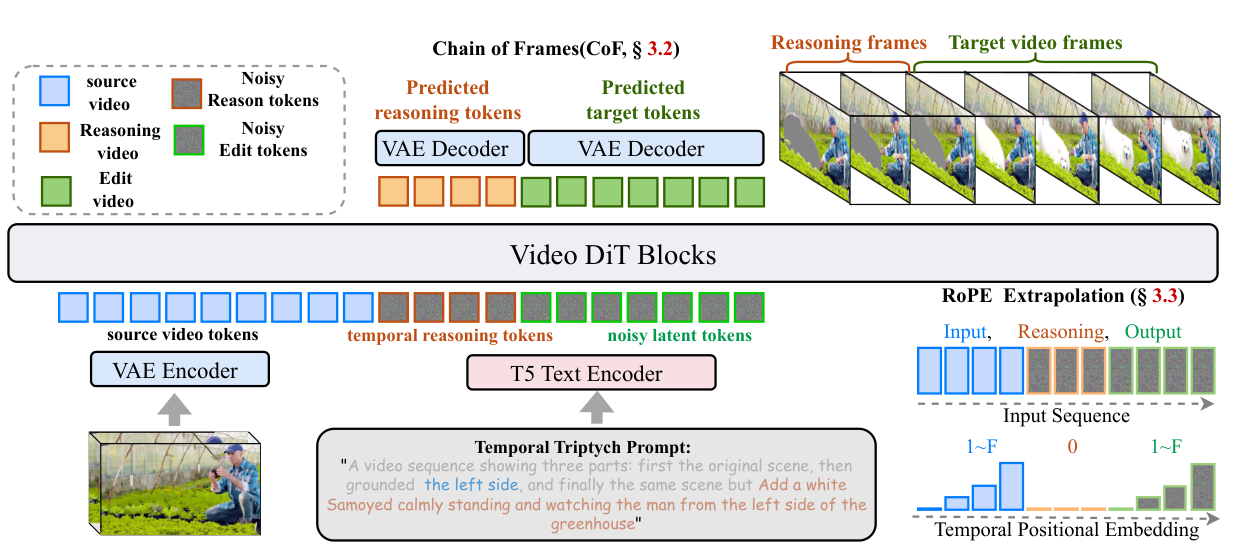
\includegraphics[keepaspectratio,alt={源内容、区域表示和目标内容的链式组织 （论文示意，来源：videocof）}]{assets/seedance/figures/reason-edit.png}}
\caption{源内容、区域表示和目标内容的链式组织 （论文示意，来源：videocof）}
\end{figure}

这里说的区域“推理”有一个可见的中间结果，不等于语言模型内部的隐藏思维。首版先把它写成两个阶段：

\begin{verbatim}
源视频 + 指令 → 目标区域/关键帧示意
源视频 + 已确认区域 + 指令 + 参考 → 编辑后视频
\end{verbatim}

若用户已经给了可靠 mask，可直接做第二阶段；自动定位置信度低时，再让用户修正。训练生成阶段也逐渐加入预测区域，才能面对定位误差。若永远只读完美真值，推理时一点越界就可能改变生成条件。

VideoCoF 则把区域与目标放进联合去噪序列，源 latent 保持干净，区域和目标共同监督。本文先采用显式两阶段，便于检查和返工，但多付一次定位或生成开销。这是两种执行图，不能只因为都预测区域就说它们相同。

\section{编辑示例图怎样减少成对视频数据需求}\label{seedance-m17-ux7f16ux8f91ux793aux4f8bux56feux600eux6837ux51cfux5c11ux6210ux5bf9ux89c6ux9891ux6570ux636eux9700ux6c42}

还可以先从源视频选关键帧 \(I_s\)，将它编辑为 \(I_t\)，再让整段视频读取``修改前、修改后''的图像示例：

\[
p(V_t\mid V_s,c,I_s,I_t).
\]

编辑前后图像给出了一个具体变换，因而可以利用较多图像编辑数据。接到视频后，目标还要保持源运动；若只按修改后图片重新生成另一段动作，就没有完成从示例传播编辑的任务。

关键帧能说明正面外观，不一定说明转身后的背面，也未必覆盖后半段才出现的道具或多角色关系。这些情况仍需增加参考或编辑示例。若各角度独立编辑后直接拼接，单帧都合理，时间上也可能互相冲突。

\section{损失怎样分配}\label{seedance-m17-ux635fux5931ux600eux6837ux5206ux914d}

源视频是条件，不作为普通噪声目标。目标视频使用有效位置上的流匹配损失；若训练区域预测，再给区域头或区域 latent 单独监督：

\[
\mathcal{L}=\mathcal{L}^{\mathrm{target}}_{\mathrm{flow}}
+\lambda_r\mathcal{L}_{\mathrm{region}}
+\lambda_p\mathcal{L}_{\mathrm{preserve}}.
\]

保持项的前提是空间仍可对齐。改相机、视角或大姿态时，逐像素拉回原图可能正好阻止目标变化。区域预测和生成质量因此要分别看，保持误差小也可能只是模型选择了不编辑。

\section{最终输出怎样保护已通过的部分}\label{seedance-m17-ux6700ux7ec8ux8f93ux51faux600eux6837ux4fddux62a4ux5df2ux901aux8fc7ux7684ux90e8ux5206}

严格局部任务最后可只合成允许区域，外部取原像素；需保留的音轨直接取原采样。这样保持由输出合成实现，不再要求有损 VAE 在未编辑处做到无损重建。

语义编辑则允许更多上下文变化，应按身份、动作、几何与连贯性验收。先做``颜色/局部替换''，再做视角和光照任务，能更清楚地定位接口是否有效。

机制代码见 \hyperref[code-condition-unit]{condition\_unit.py} 与 \hyperref[code-local-edit]{local\_edit.py}，均只作说明。真实统一条件实现读 \href{https://github.com/ali-vilab/VACE}{VACE}，区域中间表示读 \href{https://github.com/knightyxp/VideoCoF}{VideoCoF}，图像编辑迁移到视频的方法读 \href{https://vincie-next.github.io/}{VINCIE-NExT}。它们提供可借鉴机制，迁入联合音视频主干仍需要新适配和训练。

% Imported from topics/video-generation/seedance-2.5/av-editing-spec.md
\chapter{音视频编辑状态与四类掩码}\label{seedance-m23}
\moduleinfo{M23}{候选设计与工程选型；组合效果待验证}{\hyperref[src-vace]{\texttt{vace}}、\hyperref[src-videocof]{\texttt{videocof}}、\hyperref[src-vincie-next]{\texttt{vincie-next}}、\hyperref[src-ltx-2]{\texttt{ltx-2}}、\hyperref[src-ltx-original-code]{\texttt{ltx-original-code}}、\hyperref[src-ltx-original-model]{\texttt{ltx-original-model}}}

接着把源条件扩到音视频：分别决定哪条流、哪个区间需要更新，最终在哪个表示域保持原内容。

同样叫局部编辑，改外套与改台词需要更新的模态并不相同。前者可能要求声音逐采样保持；后者则要改变声音并让嘴形跟上。因此先定义保留规则，再决定视频和声音中哪些位置进入去噪，不能从“局部”二字直接推出同一种输入。

这里仍在同一音视频主干上增加干净源条件和区域支路。严格外区由最终合成保持，几何不再对齐的任务另按语义检查。下面把这个候选过程逐步写出，尚未经过实际训练。

\section{一次编辑保存四类mask}\label{seedance-m23-ux4e00ux6b21ux7f16ux8f91ux4fddux5b58ux56dbux7c7bmask}

{\def\LTcaptype{table} % do not increment counter
\small\setlength{\tabcolsep}{3pt}\renewcommand{\arraystretch}{1.18}
\begin{longtable}[]{@{}
  >{\raggedright\arraybackslash}p{(\linewidth - 4\tabcolsep) * \real{0.1900}}
  >{\raggedright\arraybackslash}p{(\linewidth - 4\tabcolsep) * \real{0.3900}}
  >{\raggedright\arraybackslash}p{(\linewidth - 4\tabcolsep) * \real{0.4200}}@{}}
\toprule\noalign{}
\begin{minipage}[b]{\linewidth}\raggedright
名称
\end{minipage} & \begin{minipage}[b]{\linewidth}\raggedright
决定什么
\end{minipage} & \begin{minipage}[b]{\linewidth}\raggedright
典型形状
\end{minipage} \\
\midrule\noalign{}
\endhead
\bottomrule\noalign{}
\endlastfoot
条件可见性 & query允许读哪些源/参考/历史 & 逻辑关系或块稀疏结构 \\
去噪更新 & 采样器改变哪些目标位置 & 视频 \(B,N_v,1\)，音频 \(B,N_a,1\) \\
监督有效位 & 哪些预测计入训练损失 & 与目标token对齐 \\
最终合成alpha & 交付文件替换哪些像素/采样 & 像素帧网格或波形采样轴 \\
\end{longtable}
}

四种 mask 虽可从同一用户范围派生，作用却不相同。VAE 有时间感受野，模型工作区往往比最终替换区大；甚至可以先生成整个目标，再只合成一个小区域。共用一份不加说明的 mask，就把这些区别抹掉了。

\section{从时间戳到latent不是简单除八}\label{seedance-m23-ux4eceux65f6ux95f4ux6233ux5230latentux4e0dux662fux7b80ux5355ux9664ux516b}

用户区间使用共同媒体时钟的半开区间 \([a,b)\)。视频帧由PTS选择，音频按采样时间选择；VFR视频先建立真实重采样映射。

latent先保存原生位置网格边界，工作区选择与 \([a,b)\) 相交的token，再依据encoder、源塔与decoder的实际感受野扩张。位置网格只用于时间对应，不表示某个token只依赖或只影响这段像素。空间mask按主体跟踪传播，并考虑下采样与卷积覆盖；只取中心点可能漏掉边缘。

还要看解码端的依赖。原系列视频 encoder 时间因果，并不推出 decoder 不读未来；直接逐块解码，未必等于整段解码。因此首版先保存完整 latent、统一解码再合成。若以后分块，还需按实际感受野安排 halo 和边界处理。

\section{源条件保持干净，目标可以全部去噪}\label{seedance-m23-ux6e90ux6761ux4ef6ux4fddux6301ux5e72ux51c0ux76eeux6807ux53efux4ee5ux5168ux90e8ux53bbux566a}

源条件先拆待变与保留部分，各自编码；参考与目标也独立编码。首版在工作窗口内对目标完整去噪，再在像素端处理严格保持，避免先假设每个保留像素都对应一个完全独立的已知 latent。

已知区重噪覆盖是可选的第二种策略：

\[
z_{\sigma}^{\mathrm{known}}=(1-\sigma)z_0^{\mathrm{source}}+
\sigma\epsilon^{\mathrm{fixed}}.
\]

若采用已知区覆盖，每步要沿同一条固定噪声路径，训练中也见过相同方式。它和干净源条件不同，仍不能保证像素无损。边界像素共享 latent 时，可先让边界 token 进入工作区，最后按允许区域合成。

\section{先区分四种音轨任务}\label{seedance-m23-ux5148ux533aux5206ux56dbux79cdux97f3ux8f68ux4efbux52a1}

{\def\LTcaptype{table} % do not increment counter
\small\setlength{\tabcolsep}{3pt}\renewcommand{\arraystretch}{1.18}
\begin{longtable}[]{@{}
  >{\raggedright\arraybackslash}p{(\linewidth - 6\tabcolsep) * \real{0.1600}}
  >{\raggedright\arraybackslash}p{(\linewidth - 6\tabcolsep) * \real{0.2800}}
  >{\raggedright\arraybackslash}p{(\linewidth - 6\tabcolsep) * \real{0.2800}}
  >{\raggedright\arraybackslash}p{(\linewidth - 6\tabcolsep) * \real{0.2800}}@{}}
\toprule\noalign{}
\begin{minipage}[b]{\linewidth}\raggedright
编辑任务
\end{minipage} & \begin{minipage}[b]{\linewidth}\raggedright
视频目标
\end{minipage} & \begin{minipage}[b]{\linewidth}\raggedright
音频目标
\end{minipage} & \begin{minipage}[b]{\linewidth}\raggedright
交付策略
\end{minipage} \\
\midrule\noalign{}
\endhead
\bottomrule\noalign{}
\endlastfoot
换衣/换背景，声音保持 & 工作区生成 & 无；源音轨干净条件 & 外区原像素＋完整原音轨 \\
修改台词 & 嘴形及允许影响区域生成 & 指定台词区间生成 & 原音轨外区＋新台词区间 \\
改动作及对应音效 & 动作与接触相关区域生成 & 相应音效工作区生成 & 声画统一验收，允许必要上下文变化 \\
整体换风格或相机 & 语义约束下生成 & 按任务保持或重生 & 几何/身份/同步验收，不能要求全部外区逐像素不变 \\
\end{longtable}
}

台词任务还要给转录、speaker、时间预算和声音参考。新句子若长于原片段，就必须重写或明确允许延长；偷偷截掉字、任意拉伸声音，都没有满足原来的逐字与时间要求。

\section{固定音频与局部音频怎样参加去噪}\label{seedance-m23-ux56faux5b9aux97f3ux9891ux4e0eux5c40ux90e8ux97f3ux9891ux600eux6837ux53c2ux52a0ux53bbux566a}

固定音轨每步使用同一干净音频latent，噪声时间为0，声音流参与隐藏状态计算，音频损失与latent更新关闭。局部重生成时，仅活动区间加噪和更新，外部为干净条件。

候选分布为：

\[
\sigma_i^a=A_i\sigma,\quad
z_i^a=(1-\sigma_i^a)z_{0,i}^a+\sigma_i^a\epsilon_i^a.
\]

\(A_i\)表示音频工作区。它必须从codec覆盖区间派生，不能把每个40毫秒位置视为互不重叠的独立波形块。混响与卷积上下文也会跨过最终剪辑边界。

状态构造的机制代码见 \hyperref[code-condition-state]{condition\_state.py}，仅作说明。这里再强调一个依赖：固定输入音频 latent 后，AV 交互仍读取每步的视频，所以深层声音特征不固定，默认仍逐步重算。

\section{自动区域错误怎样回退}\label{seedance-m23-ux81eaux52a8ux533aux57dfux9519ux8befux600eux6837ux56deux9000}

无用户mask时，先用指令定位、检测与跟踪产生候选区域。区域ID、置信度和目标主体槽一起进入第二阶段。定位错误与生成错误分别标注，低置信目标可退回关键帧修正。

定位输出也有误差，生成阶段必须见过它。训练可混入可控腐蚀、膨胀、漂移以及真实预测区域，避免始终用完美 mask 训练。灰度区域生成和分割头是两种实现，首版先固定其一，使输出与监督含义对应。

\section{遮挡、阴影与运动边界怎样定义}\label{seedance-m23-ux906eux6321ux9634ux5f71ux4e0eux8fd0ux52a8ux8fb9ux754cux600eux6837ux5b9aux4e49}

例如手或道具挡住外套，mask 就还要记录衣服的可见部分、遮挡物归属和边界置信度。若遮挡物应保持，可单独复用原 alpha；若要生成新姿态，被遮住区域又可能必须重建。保持范围因此要随任务改变。

颜色变化若需要改变反光和阴影，应显式增加允许影响区域。若用户只批准外套像素，输出可以严格局部合成，但不能同时保证全局光照物理一致。

\section{交付合成的保证范围}\label{seedance-m23-ux4ea4ux4ed8ux5408ux6210ux7684ux4fddux8bc1ux8303ux56f4}

合成放在高质量工作表示上：视频按 alpha 取源帧或生成帧，音频按原采样率和时间取相应波形，之后统一编码混流。这里保持的是编码前外区；有损重编码会再次改变表示，所以不能连带保证文件字节或最终解码像素完全相同。

音频交界可以交叉淡化，淡化区必须包含在允许编辑时间内。声学连续性与逐采样外区保持冲突时，需要在任务规格中明确哪项优先，不能把淡化悄悄扩到禁止区间。

绿幕输出还需要独立前景alpha、边缘去色溢出和颜色管理。背景替换后的人物光照若需变化，应放入可编辑条件；单独输出一个绿色背景不是可靠matte。

\section{怎样判断改对而不是没改}\label{seedance-m23-ux600eux6837ux5224ux65adux6539ux5bf9ux800cux4e0dux662fux6ca1ux6539}

评价时把目标变化与外区保持放在一起，再看边界、身份、动作、台词、speaker 和声画偏差。只让保持误差变小，复制整段源视频也能做到，因此它不能单独证明编辑有效。

真实条件组织看 \href{https://github.com/ali-vilab/VACE}{VACE}，区域中间表示看 \href{https://github.com/knightyxp/VideoCoF}{VideoCoF}。已有LTX \href{https://github.com/Lightricks/LTX-2/blob/bd92a5f408eb8c99f8c05e9fe2fcaaec8b56b638/packages/ltx-trainer/src/ltx_trainer/training_strategies/video_to_video.py}{视频IC-LoRA策略} 是实现起点；上述音频状态、区域损失和最终合成需要另外接入。

% Imported from topics/video-generation/seedance-2.5/geometry-control.md
\chapter{M18 白模、相机与场景记忆}\label{seedance-m18}
\moduleinfo{M18}{候选设计与工程选型；组合效果待验证}{\hyperref[src-geometry-as-context]{\texttt{geometry-as-context}}、\hyperref[src-vace]{\texttt{vace}}、\hyperref[src-ltx-2]{\texttt{ltx-2}}}


让模型参考一张房间图，可以保持大致风格，却未必能记住相机转过去后被遮挡的桌子。空间控制需要回答两个问题：当前画面应该由哪个相机看到，以及之前不可见的物体在三维场景中处于什么位置。

白模和几何上下文提供了两类互补信息。前者把已知布局和运动先渲染出来，后者让模型显式读取或预测深度等结构。两者都可以帮助生成，但都不能把``看起来有三维感''当成几何真值。

\section{白模应输出哪些条件}\label{seedance-m18-ux767dux6a21ux5e94ux8f93ux51faux54eaux4e9bux6761ux4ef6}

对于自有三维场景，优先导出同步的 clay RGB、深度、法线、实例 ID、相机内外参和物体轨迹。相机单位、轴方向、深度范围、镜头畸变和帧时间必须固定。

深度和法线可以作为规范化图像通过视觉条件支路编码，但它们有不同数值含义：相对深度不等于米制深度，法线通道也不等于普通 RGB。条件需附 modality/type 标记与有效区域，避免模型把控制图当作目标材质。

真实视频估计的深度与相机没有精确渲染的可信度。把估计结果用作弱条件时，应保留置信度、遮挡和缺失值，不通过随意补零把未知表面变成真实平面。

\section{相机射线怎样表达视角}\label{seedance-m18-ux76f8ux673aux5c04ux7ebfux600eux6837ux8868ux8fbeux89c6ux89d2}

给定像素齐次坐标 \(u\)、相机内参 \(K\)、相机到世界旋转 \(R\) 和相机中心 \(o\)，归一化世界射线方向为：

\[
d(u)=\frac{RK^{-1}u}{\lVert RK^{-1}u\rVert_2}.
\]

Plücker 表示将方向与矩联合：

\[
r(u)=[d(u),o\times d(u)].
\]

它把每个像素``从哪里看向哪里''作为条件。相机平移尺度改变会影响矩，因此必须与场景单位一致；只有旋转正确、位移单位错误，同样会让轨迹失真。

候选实现将射线图按视觉 latent 网格汇聚，再经独立投影进入相机支路。相机与深度已知时，不让模型先重新猜一遍它们。

\section{几何上下文怎样成为记忆}\label{seedance-m18-ux51e0ux4f55ux4e0aux4e0bux6587ux600eux6837ux6210ux4e3aux8bb0ux5fc6}

另一条路线是让同一模型处理交错的 RGB、几何和下一视角任务：

\begin{verbatim}
当前图像 → 当前几何 → 指定相机下的下一图像 → 下一几何 → …
\end{verbatim}

\begin{figure}
\centering
\pandocbounded{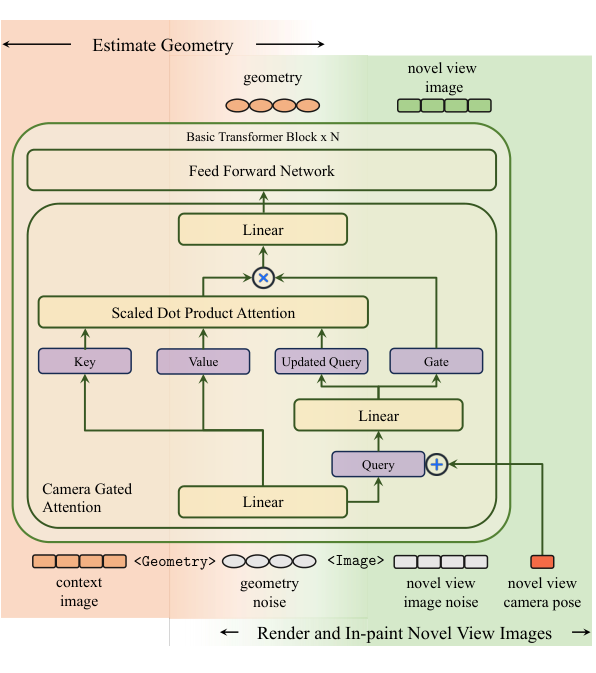
\includegraphics[keepaspectratio,alt={几何任务、图像任务与相机门控注意力 （论文示意，来源：geometry-as-context）}]{assets/seedance/figures/geometry-context.png}}
\caption{几何任务、图像任务与相机门控注意力 （论文示意，来源：geometry-as-context）}
\end{figure}

图中相机影响 query 和输出门控，使模型在估计几何和生成新视角时使用不同条件。几何上下文可以让过去内容以显式结构参与后续生成，但同时增加序列长度；训练时随机去掉一部分几何上下文，可让模型兼容只用图像的路径。

Geometry-as-Context 的公开路线使用自己的交错生成基座，不能直接加载为 LTX 或 Wan 的插件。候选工程先实现已知白模与相机条件，只有场景导航确有收益时，再研究预测几何的辅助头或交错任务。

\section{场景记忆不要只存第一帧}\label{seedance-m18-ux573aux666fux8bb0ux5fc6ux4e0dux8981ux53eaux5b58ux7b2cux4e00ux5e27}

长期记忆可以分为静态结构、动态主体状态和视觉证据。静态结构包括相机坐标和固定物体，动态状态包括角色当前位置、拿着什么道具，视觉证据包括可重访视角的关键帧、深度和置信度。

每个新镜头从相机距离、可见性和新鲜度检索若干关键帧，而不是把所有旧视频无上限地拼入 attention。模型生成后，对高置信区域更新记忆，对新露出或矛盾区域保留不确定性，避免一次错误被写成永久场景真值。

首版记忆是外部数据结构与条件检索，不声称已完成三维重建。若使用深度重投影合成，需要处理遮挡和新露出区域；这些区域仍由生成器补全，并单独标记为新推断内容。

\section{怎样测真正的空间保持}\label{seedance-m18-ux600eux6837ux6d4bux771fux6b63ux7684ux7a7aux95f4ux4fddux6301}

相机离开后返回同一位置，是很重要的检查。比较重访视角中的物体存在、位置、颜色和遮挡关系，往往比看连续两帧更能暴露``场景记忆''失败。

还应比较已知轨迹跟随、相机方向错误、动态物体与静态背景分离，以及深度置信度低时的退化。只有几何允许对齐的区域才使用重投影像素误差，遮挡和新露出区域单独评价。

极简射线表示见 \hyperref[code-camera-rays]{camera\_rays.py}。真实控制条件组织可读 \href{https://github.com/ali-vilab/VACE}{VACE}，几何交错建模的机制来自 Geometry-as-Context；本方案没有声称已经实现相同的长程三维效果。

\part{生成主干与联合模块}
% Imported from algorithms/multimodal-position/README.md
\chapter{M04 多模态位置编码与媒体时钟}\label{seedance-m04}
\moduleinfo{M04}{基础方法与机制解释}{\hyperref[src-rope]{\texttt{rope}}、\hyperref[src-seedance-1.0]{\texttt{seedance-1.0}}、\hyperref[src-long-context-tuning]{\texttt{long-context-tuning}}、\hyperref[src-wan21-code]{\texttt{wan21-code}}、\hyperref[src-vincie-code]{\texttt{vincie-code}}}


Transformer 把输入组织成 token 序列，但一维排列顺序不足以描述视频结构。视觉 token 同时位于某个时间、某行和某列；文本 token 位于一句话中；多个镜头还各有自己的描述。多模态位置编码要保留这些不同的位置含义，让注意力知道内容之间的相对关系。

\section{RoPE 怎样把位置放进点积}\label{seedance-m04-rope-ux600eux6837ux628aux4f4dux7f6eux653eux8fdbux70b9ux79ef}

RoPE 将一对特征维度看成平面向量，按位置旋转。设旋转矩阵为：

\[
R(\phi)=\begin{bmatrix}
\cos\phi&-\sin\phi\\
\sin\phi&\cos\phi
\end{bmatrix}.
\]

位置为 \(m\) 的 query 和位置为 \(n\) 的 key，分别变为：

\[
q'_m=R(m\omega)q_m,\qquad k'_n=R(n\omega)k_n.
\]

由于旋转矩阵满足组合关系，点积可以写成：

\[
(q'_m)^\top k'_n=q_m^\top R((n-m)\omega)k_n.
\]

这样，显式引入的位置信息依赖相对距离 \(n-m\)。保持内容向量不变，同时把两个位置都平移 7，点积就保持不变。不过，网络中的内容向量本身已经受上下文影响，不能进一步推成``整个网络只依赖相对位置''。

不同特征对使用不同频率，常见形式为 \(\omega_i=b^{-2i/d_{\mathrm{rot}}}\)。旋转作用于投影后的 Q/K，位于注意力点积之前；V 通常不旋转，因为标准 RoPE 通过改变关注权重来引入位置。

\section{三维位置怎样进入同一个注意力头}\label{seedance-m04-ux4e09ux7ef4ux4f4dux7f6eux600eux6837ux8fdbux5165ux540cux4e00ux4e2aux6ce8ux610fux529bux5934}

注意力张量常写成 \codepath{B,h,N,d_h}：批大小、头数、token 数和单头维度。三维 RoPE 将最后的特征维度划给时间、高度、宽度三个轴，而不是复制三份 token。

\[
d_t+d_y+d_x\le d_h.
\]

每一段需要能成对旋转，通常取偶数；未参与旋转的通道可以原样保留。例如 \(d_h=12\)，三个轴各分 4 维。视觉 token 坐标为 \((t,y,x)\)，时间段使用 \(t\)，空间两段分别使用 \(y\) 和 \(x\)。

不同实现可能按相邻维配对，也可能将前后半段配对；配置中的数字也可能表示通道数或频率对数。迁移模型时，维度总和一致仍不足以证明布局兼容。

\section{多镜头怎样交错排列}\label{seedance-m04-ux591aux955cux5934ux600eux6837ux4ea4ux9519ux6392ux5217}

多镜头场景可以组织为``镜头描述、镜头视觉、下一镜头描述、下一镜头视觉''的交错序列。镜头内保留文本与视觉的位置关系，镜头之间再增加偏移。

\begin{figure}
\centering
\pandocbounded{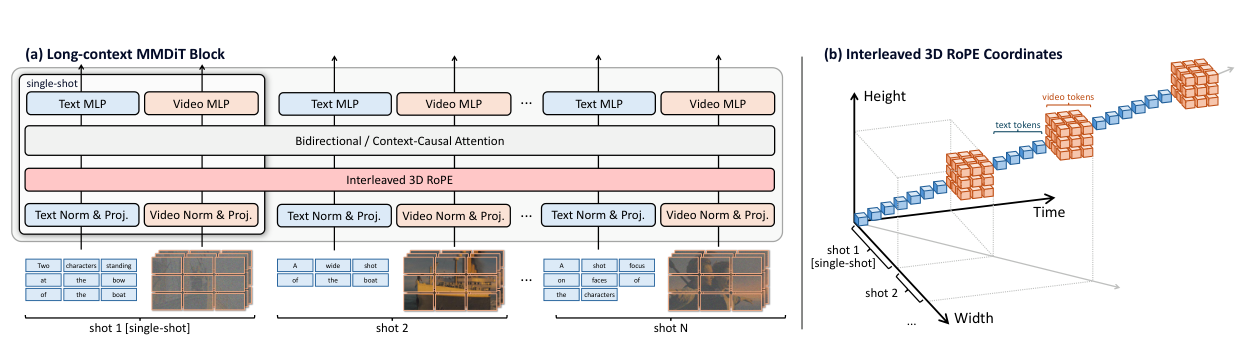
\includegraphics[keepaspectratio,alt={多镜头上下文与交错位置的组织 （论文示意，来源：long-context-tuning）}]{assets/seedance/figures/multishot-positions.png}}
\caption{多镜头上下文与交错位置的组织 （论文示意，来源：long-context-tuning）}
\end{figure}

图中左侧是跨镜头处理文本与视频的结构，右侧展示位置坐标如何随镜头追加。这种组织让相邻镜头具有不同的绝对位置，同时保留每个镜头内部原有的相对结构。

文本没有真实空间坐标，可以使用一维位置，或将同一个序列位置映射到多个轴。若频率和布局与原一维 RoPE 兼容，多轴形式可以退化为一维；若每轴重新起一组频率，则不一定与原实现完全相同。

\section{坐标、归属和可见性是三件事}\label{seedance-m04-ux5750ux6807ux5f52ux5c5eux548cux53efux89c1ux6027ux662fux4e09ux4ef6ux4e8b}

坐标回答``token 在哪里''；归属回答``这段描述或参考属于哪个镜头、哪个角色''；注意力掩码回答``哪些 token 允许互相读取''。三者需要一起设计。

例如，一张参考图只约束第二个镜头中的角色 A。即使为它设置了独立位置，也不能保证模型只把它用于角色 A。还需要角色和镜头绑定，必要时用显式 mask 限定可见范围。RoPE 只改变分数，并不会自动把不允许的连接设为负无穷。

同样，一组相同坐标既可以用于联合生成，也可以配合镜头间因果 mask 用于续写。因果性由信息流决定，不能仅凭坐标递增来判断。

\section{实现时最容易忽略的时间单位}\label{seedance-m04-ux5b9eux73b0ux65f6ux6700ux5bb9ux6613ux5ffdux7565ux7684ux65f6ux95f4ux5355ux4f4d}

视频帧号不是通用时间。固定 24 fps 的第 48 帧约对应两秒，可变帧率视频则需要读取实际时间戳；音频编码器可能每秒输出另一数量的 token。做音视频对齐时，应先把各模态位置映射到同一个物理时间轴，再决定编码方式。

检查一个位置编码实现，可以先验证坐标展平与还原是否一一对应，再检查 padding 是否被排除，最后测试同移坐标的点积性质。真正扩展到长视频时，还需要观察生成质量：位置编码能计算更远的坐标，不代表模型已经学会在这些坐标范围内保持角色、动作和剧情。

\section{从极简代码到真实实现}\label{seedance-m04-ux4eceux6781ux7b80ux4ee3ux7801ux5230ux771fux5b9eux5b9eux73b0}

对一对特征维度旋转时，真正改变的是 Q/K 的最后一维：

\begin{verbatim}
even, odd = x[..., 0::2], x[..., 1::2]
rotated_even = even * cos - odd * sin
rotated_odd = even * sin + odd * cos
\end{verbatim}

按三轴拆分再拼回的示例见 \hyperref[code-rope]{rope.py}。示例采用相邻维配对和各轴独立频率；真实 checkpoint 的布局应查 \href{https://github.com/Wan-Video/Wan2.1/blob/9737cba9c1c3c4d04b33fcad41c111989865d315/wan/modules/model.py}{Wan rope\_apply} 或 \href{https://github.com/ByteDance-Seed/VINCIE/blob/97cd2c5701e694dabcfea320c0cf59893d427fab/models/dit/rope.py}{VINCIE 多模态 RoPE}，不能仅看输出维数相同。

% Imported from algorithms/diffusion-transformers/README.md
\chapter{时空 DiT 与多模态注意力}\label{seedance-m03}
\moduleinfo{M03}{基础方法与机制解释}{\hyperref[src-seedance-1.0]{\texttt{seedance-1.0}}、\hyperref[src-dit]{\texttt{dit}}、\hyperref[src-video-dit-scaling-laws]{\texttt{video-dit-scaling-laws}}、\hyperref[src-wan-2.1]{\texttt{wan-2.1}}、\hyperref[src-wan21-code]{\texttt{wan21-code}}、\hyperref[src-vincie-code]{\texttt{vincie-code}}}

位置有了定义，再看主干内部的时空注意力怎样组织序列与文本交互。

速度回归的目标已经确定，接下来才是用什么网络表示它。主干读入 VAE 的带噪潜变量，一方面要让画面符合文本，另一方面要让同一物体沿时间连续运动。若把所有时空位置一次全部相连，成本很高；空间与时间解耦的 DiT 就把这两种交互拆到交替执行的注意力层中。

\section{潜变量怎样进入 Transformer}\label{seedance-m03-ux6f5cux53d8ux91cfux600eux6837ux8fdbux5165-transformer}

设视觉潜变量形状为 \codepath{B×C×T×H×W}。将每个网格位置投影到隐藏维度 \(d\)，得到 \codepath{B×T×H×W×d}，再按注意力层需要组织成序列。文本经过编码器后也投影到可交互的特征空间。

这里先分清 token 和通道。有的模型把多个潜位置拼成 patch，有的直接把一个位置当一个 token；后者仍要做输入投影。VAE 给出每个位置存什么，投影决定主干用多宽的特征计算，不能直接把潜通道数当成所有注意力头的维度。

\begin{figure}
\centering
\pandocbounded{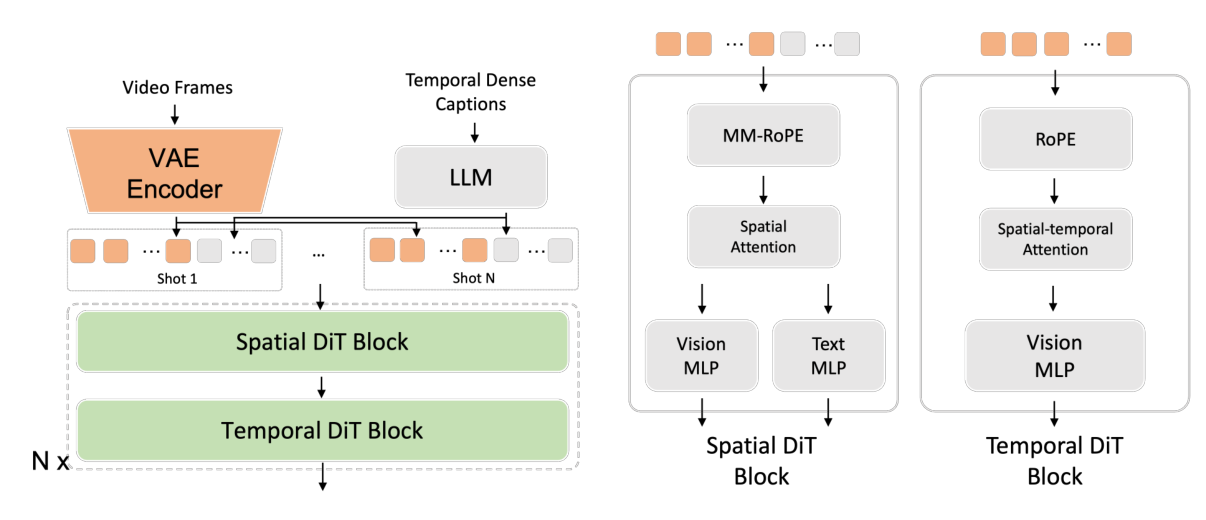
\includegraphics[keepaspectratio,alt={空间层与时间层交替组成的视频生成主干 （论文示意，来源：seedance-1.0）}]{assets/seedance/figures/spatial-temporal-dit.png}}
\caption{空间层与时间层交替组成的视频生成主干 （论文示意，来源：seedance-1.0）}
\end{figure}

按图中的顺序，空间块先让视觉与文本发生交互，时间块再沿视觉序列传播信息。于是文本的语义约束可以先进入画面，随后通过交替的时空计算影响运动。这里的分工来自具体计算图，不能只从“DiT”这个名称判断。

\section{空间层怎样融合文字与画面}\label{seedance-m03-ux7a7aux95f4ux5c42ux600eux6837ux878dux5408ux6587ux5b57ux4e0eux753bux9762}

MMDiT 再把文本也看成可更新的流。视觉与文本各自先经过归一化、QKV 投影和前馈网络，随后沿 token 维拼接，得到：

\[
Q=[Q_v;Q_c],\qquad K=[K_v;K_c],\qquad V=[V_v;V_c].
\]

拼接后，两种模态的 query 都能读取联合的 key/value，因此一次自注意力写为：

\[
Y=\operatorname{softmax}\left(\frac{QK^\top}{\sqrt{d_h}}+A\right)V.
\]

从这个式子还可以按行拆回视觉与文本输出。两种模态都给 query，就都取得更新；它们的参数仍可各自独立。因此“特征先分路、注意力时拼接”和“所有层都共享参数”不是同一个意思。

\(d_h\) 是单头维度，\(A\) 是可见性掩码。视觉 query 可以读取文本 key/value，文本 query 也能读取视觉 key/value；输出再拆回两种模态，各自经过投影、残差和前馈网络。

从输出的 query 行就能看出区别。单向文本 cross-attention 通常由视觉给 query，文本只给 key/value，因此只返回视觉序列；联合自注意力则也返回文本对应的更新。说“文本作为条件”还不够，必须继续说明文本在这次计算中究竟是哪一种角色。

反向传播也沿这整张计算图进行，不存在先看 Q、再看 K、最后看 V 的重要性排序。哪些参数更新，要看梯度路径和冻结设置。Q/K normalization 另用于控制注意力的数值尺度，与文本是否产生 query 是两个问题。

\section{时间层存在两种不同的组织方式}\label{seedance-m03-ux65f6ux95f4ux5c42ux5b58ux5728ux4e24ux79cdux4e0dux540cux7684ux7ec4ux7ec7ux65b9ux5f0f}

设每帧有 \(P=HW\) 个空间位置。最便宜的时间注意力，把同一位置在所有帧上的 token 串起来，序列形状为 \codepath{B×P} 组长度为 \(T\) 的序列。它能直接关联某个位置的时间变化，但一个物体移动到邻近位置后，需要其它空间层帮助传递信息。

另一种做法是在每帧划分空间窗口，窗口含 \(m\) 个位置，把同一窗口跨所有帧的 token 合并，形成 \(P/m\) 组长度为 \(Tm\) 的序列。这样一次注意力可以同时看到时间变化和窗口内位移。

{\def\LTcaptype{table} % do not increment counter
\small\setlength{\tabcolsep}{3pt}\renewcommand{\arraystretch}{1.18}
\begin{longtable}[]{@{}
  >{\raggedright\arraybackslash}p{(\linewidth - 4\tabcolsep) * \real{0.1900}}
  >{\raggedright\arraybackslash}p{(\linewidth - 4\tabcolsep) * \real{0.3900}}
  >{\raggedright\arraybackslash}p{(\linewidth - 4\tabcolsep) * \real{0.4200}}@{}}
\toprule\noalign{}
\begin{minipage}[b]{\linewidth}\raggedright
组织方式
\end{minipage} & \begin{minipage}[b]{\linewidth}\raggedright
注意力输入形状
\end{minipage} & \begin{minipage}[b]{\linewidth}\raggedright
可直接交互的范围
\end{minipage} \\
\midrule\noalign{}
\endhead
\bottomrule\noalign{}
\endlastfoot
逐位置时间注意力 & \codepath{B×P, T, d} & 一个空间位置上的所有帧 \\
窗口时空注意力 & \codepath{B×(P/m), Tm, d} & 一个空间窗口内的所有帧与位置 \\
\end{longtable}
}

从 \codepath{B,T,nwin,m,d} 出发，窗口时空形式先重排成 \codepath{B,nwin,T,m,d}，再合并 \(T\) 和 \(m\)。如果把 \(m\) 合进 batch，得到的依然是逐位置时间注意力，并没有窗口内空间交互。

\section{复杂度为什么要乘回帧数和位置数}\label{seedance-m03-ux590dux6742ux5ea6ux4e3aux4ec0ux4e48ux8981ux4e58ux56deux5e27ux6570ux548cux4f4dux7f6eux6570}

下面暂时不计投影和前馈，只数一个注意力头中的 token 连接。把每种序列有多长、重复几组写出来，成本就比较清楚了：

\[
\begin{aligned}
C_{\mathrm{full}}&=(TP)^2,\\
C_{\mathrm{spatial}}&=TP^2,\\
C_{\mathrm{temporal}}&=PT^2,\\
C_{\mathrm{window}}&=\frac{P}{m}(Tm)^2=PT^2m.
\end{aligned}
\]

空间加逐位置时间注意力的总成本是 \(TP^2+PT^2\)。帧内空间注意力要做 \(T\) 次，逐位置时间注意力要做 \(P\) 次，这两个重复次数不能省略。若使用窗口时空形式，时间项还要乘窗口面积 \(m\)。

取 \(T=16\)、\(H=W=32\)、\(P=1024\)、\(m=4\)，全时空有约 2.68 亿个连接，空间项约 1678 万，逐位置时间项约 26 万，窗口时空项约 105 万。连接数的大幅下降解释了结构化注意力的价值，但真实速度还受投影、前馈网络、kernel 和显存访问影响。

在乘加计为两次操作的约定下，标准 MHA 子层的粗略 FLOPs 为：

\[
8Nd^2+4N^2d.
\]

前一项来自 QKV 和输出投影，后一项来自 QK 与 AV；扩展比例为 \(r\) 的普通两层 FFN 另需约 \(4rNd^2\)。GQA 减少 K/V 头数，能降低投影和缓存开销，但每个 query 头仍然计算自己的注意力，二次交互项不会自动消失。

\section{输入变大，为什么权重可以不变}\label{seedance-m03-ux8f93ux5165ux53d8ux5927ux4e3aux4ec0ux4e48ux6743ux91cdux53efux4ee5ux4e0dux53d8}

线性层作用于最后的特征维度 \(d\)，权重不含 token 数 \(N\)。增加分辨率主要增加 token 行数，因此参数形状可以保持不变；LayerNorm 的参数同样沿特征维度定义。

不过，参数形状能复用，只回答了网络能否计算。位置范围变大、宽高比改变、物体跨窗口移动，以及长序列训练分布不同，都还会影响生成。因而分辨率适配要接着看算力与结果质量，前向不报错只是其中一步。

\section{从极简代码到真实实现}\label{seedance-m03-ux4eceux6781ux7b80ux4ee3ux7801ux5230ux771fux5b9eux5b9eux73b0}

注意力的区别首先体现在谁成为序列维。输入为 \codepath{B,T,H,W,d} 时，逐位置时间形式可以写成：

\begin{verbatim}
b, t, h, w, d = x.shape
seq = x.permute(0, 2, 3, 1, 4).reshape(b*h*w, t, d)
y = attention(seq)  # 每组只读同一位置的 T 个时间点。
\end{verbatim}

窗口时空形式则把一个窗口的时间与空间位置一起合并为长度 \(Tm\)。两种 reshape、逆变换和多模态拼接见 \hyperref[code-attention-layout]{attention\_layout.py}。真实投影与 block 可读 \href{https://github.com/Wan-Video/Wan2.1/blob/9737cba9c1c3c4d04b33fcad41c111989865d315/wan/modules/model.py}{Wan 模型}，多模态窗口实现可读 \href{https://github.com/ByteDance-Seed/VINCIE/blob/97cd2c5701e694dabcfea320c0cf59893d427fab/models/dit/blocks/attention/mmattn.py}{VINCIE attention}；它们是不同基座的结构，不能混用 checkpoint。

% Imported from algorithms/audio-video-joint/README.md
\chapter{M05 音视频联合生成}\label{seedance-m05}
\moduleinfo{M05}{基础方法与机制解释}{\hyperref[src-seedance-1.5-pro]{\texttt{seedance-1.5-pro}}、\hyperref[src-seedance-2.0]{\texttt{seedance-2.0}}、\hyperref[src-seedance-2.5-release]{\texttt{seedance-2.5-release}}、\hyperref[src-ltx-code]{\texttt{ltx-code}}、\hyperref[src-ltx-2]{\texttt{ltx-2}}、\hyperref[src-ltx-original-code]{\texttt{ltx-original-code}}}


给一段视频配上声音，与从同一个事件同时生成画面和声音，是两种不同的任务。前者可以先完成画面，再制作对白、音乐和音效；后者需要模型在生成过程中同时考虑嘴形、语调、动作节奏和环境声。原生音视频联合生成的价值，正是让两种模态共同决定``发生了什么''。

\section{两个生成分支为什么仍要交换信息}\label{seedance-m05-ux4e24ux4e2aux751fux6210ux5206ux652fux4e3aux4ec0ux4e48ux4ecdux8981ux4ea4ux6362ux4fe1ux606f}

视频和音频的数据结构不同。视频潜变量保留时间、空间和通道，音频潜变量通常以一维时间序列为主。让两者各用适合自身结构的主干，再通过联合模块交换信息，是一种可行的双分支设计。

\[
z_v\in\mathbb{R}^{B\times C_v\times T_v\times H_v\times W_v},
\qquad
z_a\in\mathbb{R}^{B\times C_a\times T_a}.
\]

视频分支预测画面速度场，音频分支预测声音速度场，文本和参考为它们提供共同条件。Seedance 1.5 Pro 采用双分支 DiT 与跨模态联合模块，但具体 codec、插入层和连接公式需要按实现确定。

\begin{figure}
\centering
\pandocbounded{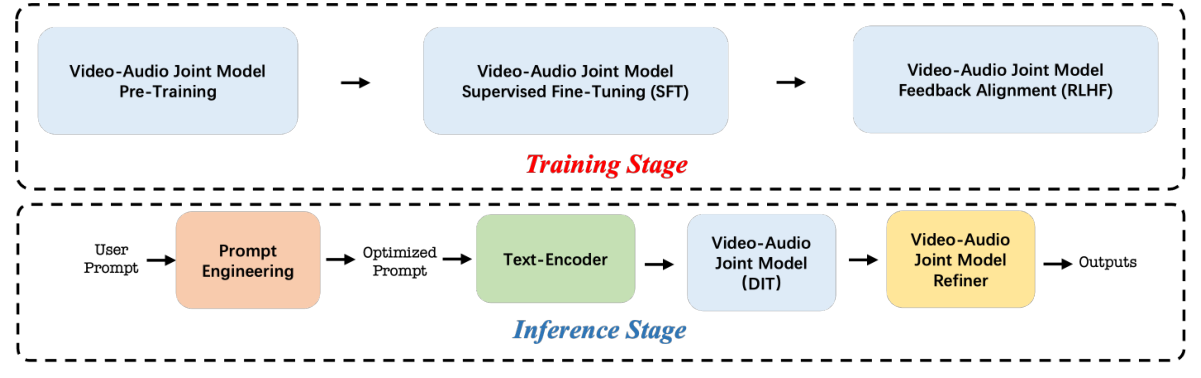
\includegraphics[keepaspectratio,alt={音视频模型的训练与生成流程 （论文示意，来源：seedance-1.5-pro）}]{assets/seedance/figures/audio-video-pipeline.png}}
\caption{音视频模型的训练与生成流程 （论文示意，来源：seedance-1.5-pro）}
\end{figure}

训练部分先学习联合分布，再用高质量样本和反馈优化；生成部分从提示改写、文本编码进入联合模型，必要时经过精修。图中呈现的是整体流程，不能用它代替具体交换模块的定义。

如果两个分支完全独立，即便输入同一个提示，也可能出现``画面里已经落地，声音还没响''或``人嘴闭着但仍在说话''。联合模块需要让一个模态读取另一个模态的当前生成状态。

\section{一种明确的交换方式}\label{seedance-m05-ux4e00ux79cdux660eux786eux7684ux4ea4ux6362ux65b9ux5f0f}

可以在部分层加入双向交叉注意力：

\[
\Delta h_v=\operatorname{Attn}(Q_v,K_a,V_a),
\qquad
\Delta h_a=\operatorname{Attn}(Q_a,K_v,V_v).
\]

再通过门控残差把增量加回各分支。这个公式是双分支方案的一种选择，并不意味着所有联合模型都采用相同结构。门控可以从零开始，使新模块在训练初期不干扰已有生成能力。

双向交换仍然有计算代价。若视频和音频 token 数分别为 \(N_v,N_a\)，一次完整交互的连接规模约为 \(N_vN_a\)。可以限制读取相近时间、先池化摘要，或者减少交换层，但每种压缩都会牺牲一部分对齐信息。

\section{同步依赖物理时间，不依赖相同索引}\label{seedance-m05-ux540cux6b65ux4f9dux8d56ux7269ux7406ux65f6ux95f4ux4e0dux4f9dux8d56ux76f8ux540cux7d22ux5f15}

假设视频为 24 fps，音频编码器每秒输出 50 个 token。两秒事件附近对应视频帧号 48、音频 token 号 100，它们的索引显然不能直接一一对应。还要考虑 VAE 时间压缩、音频 codec 的感受野、首帧规则和固定延迟。

可靠的做法是为每个 token 保存其覆盖的物理时间区间，并统一时间起点。局部跨模态 attention 才能按照``相隔多少毫秒''建立邻域，而不是按两个不相容的 token 序号建立邻域。

数据预处理也必须真正重采样。修改采样率或 fps 的元数据不会自动改变波形和帧序列；错误的时间戳会把输入错位变成模型必须学习的噪声。

\section{一套具体的共同表示}\label{seedance-m05-ux4e00ux5957ux5177ux4f53ux7684ux5171ux540cux8868ux793a}

LTX-2原系列提供了可参照的完整表示：视频latent为128通道，时间压缩8倍、空间各32倍；音频codec可保留 \codepath{B,8,Ta,16}，再展平为每时间位置128维，约25个时间位置/秒。音频输入使用16kHz的mel表示，经vocoder输出24kHz立体声；采样率与latent时间率是不同量。

这些配置应与同一系列的文本、归一化、调制和scheduler配套。视频压缩首帧规则要求内部帧数满足 \(F=1+8k\)，音频时长则按共同媒体时钟处理。采用这类现成联合主干后，新任务主要增加参考与源条件接口；无需再假设任意视频latent都能直接与一个音频生成器相接。

\section{两种损失怎样配平}\label{seedance-m05-ux4e24ux79cdux635fux5931ux600eux6837ux914dux5e73}

令噪声时间 \(t=0\) 对应数据、\(t=1\) 对应噪声。一种基础联合目标为：

\[
\mathcal{L}=\lambda_v\operatorname{MSE}(u_v,\epsilon_v-z_v)
+\lambda_a\operatorname{MSE}(u_a,\epsilon_a-z_a).
\]

两项应先分别按有效元素归一化，再观察损失量级与梯度范数。简单地把所有元素求和，会让 token 更多或数值尺度更大的模态主导更新。权重也不能只根据通道数决定。

混合训练中，缺少音轨与真实静音必须分开。缺音轨样本不计算音频目标损失；静音样本则有有效的音频目标。若把缺失音频统一当成静音，就会教模型在有声事件中保持安静。对白、环境音和音乐也应分别描述，画面中无法判断的台词不能被自动补成事实。

\section{怎样判断联合生成是否值得}\label{seedance-m05-ux600eux6837ux5224ux65adux8054ux5408ux751fux6210ux662fux5426ux503cux5f97}

口型、敲击、落地和脚步可以分别测量视觉事件与声音起点的偏差，单位统一为毫秒，同时人工复听语言、音色和情绪。同步分数之外，还要检查联合训练是否损伤画面的动作幅度或文本遵循，以及音频是否出现失真、杂音和无关音乐。

如果业务主要使用旁白，视频生成后配音和确定性混流往往已经可用。人物对白、唱歌和精确动作音效对联合建模的收益更大，但也需要更干净的对齐数据。是否增加音频分支，应由这些具体任务的质量与成本决定。

\section{从极简代码到真实实现}\label{seedance-m05-ux4eceux6781ux7b80ux4ee3ux7801ux5230ux771fux5b9eux5b9eux73b0}

双向交互需要两边都读取更新前的状态，否则执行顺序本身会引入不对称：

\begin{verbatim}
delta_video = attention(video_q, audio_k, audio_v)
delta_audio = attention(audio_q, video_k, video_v)
new_video = video + delta_video
new_audio = audio + delta_audio
\end{verbatim}

单头教学版本见 \hyperref[code-audio-video-exchange]{audio\_video\_exchange.py}；真实联合模块可读 \href{https://github.com/Lightricks/LTX-2/blob/daa6b16fc7f0f1628f2c9e36a303e3312b333cc6/packages/ltx-core/src/ltx_core/model/transformer/transformer.py}{LTX 的 BasicAVTransformerBlock}。它包含自己的调制、位置和条件接口，应作为独立音视频工程阅读，而不是直接当作 Wan 的音频插件。

% Imported from topics/video-generation/seedance-2.5/adapter-contract.md
\chapter{新增模块的维度与接入契约}\label{seedance-m21}
\moduleinfo{M21}{候选设计与工程选型；组合效果待验证}{\hyperref[src-ltx-2]{\texttt{ltx-2}}、\hyperref[src-ltx-original-code]{\texttt{ltx-original-code}}、\hyperref[src-ltx-original-model]{\texttt{ltx-original-model}}、\hyperref[src-vace]{\texttt{vace}}}

前面分别讲了注意力和音视频交换，这里固定一个公开替代基座，逐层核对候选条件支路的维度与插入顺序。

已有音视频主干之后，怎样增加控制而不把原来所有接口重做？先把原权重的输入约定固定，再定义新条件从哪里读、以什么维度加回来。下面以 LTX-2 原系列 19B 开发模型逐层写出这种关系。原生配置来自公开元数据，新增宽度、层位与训练方式则是未验证的候选。

\section{先固定一套确切的主干}\label{seedance-m21-ux5148ux56faux5b9aux4e00ux5957ux786eux5207ux7684ux4e3bux5e72}

选用 \codepath{ltx-2-19b-dev.safetensors}，保留配套视频/音频codec、Gemma文本特征、连接器、归一化和采样器。模型配置为48个联合块，视频宽度4096、32头且每头128维，音频宽度2048、32头且每头64维。两流输入与输出token均为128维。

这组权重使用split RoPE、双精度频率计算，时间调制倍率1000，AV交互调制倍率1000。构造器提供的默认值不能代替权重配置；新参考支路也不改写原有RoPE。

{\def\LTcaptype{table} % do not increment counter
\small\setlength{\tabcolsep}{3pt}\renewcommand{\arraystretch}{1.18}
\begin{longtable}[]{@{}
  >{\raggedright\arraybackslash}p{(\linewidth - 4\tabcolsep) * \real{0.1900}}
  >{\raggedright\arraybackslash}p{(\linewidth - 4\tabcolsep) * \real{0.3900}}
  >{\raggedright\arraybackslash}p{(\linewidth - 4\tabcolsep) * \real{0.4200}}@{}}
\toprule\noalign{}
\begin{minipage}[b]{\linewidth}\raggedright
对象
\end{minipage} & \begin{minipage}[b]{\linewidth}\raggedright
进入模型前
\end{minipage} & \begin{minipage}[b]{\linewidth}\raggedright
进入联合块后
\end{minipage} \\
\midrule\noalign{}
\endhead
\bottomrule\noalign{}
\endlastfoot
视频目标 & \(B\times N_v\times128\) & \(B\times N_v\times4096\) \\
音频目标 & \(B\times N_a\times128\) & \(B\times N_a\times2048\) \\
文本连接器输出 & \(B\times L\times3840\) & 原生投影分别到4096/2048 \\
视频坐标边界 & \(B\times3\times N_v\times2\) & 原生时空位置编码 \\
音频坐标边界 & \(B\times1\times N_a\times2\) & 原生时间位置编码 \\
每token噪声状态 & \(B\times N_m\) & 原生AdaLN与AV调制 \\
\end{longtable}
}

\(B\)为batch，\(N_v,N_a,L\)为视频、音频、文本长度。坐标最后一维保存原生位置网格的起止；视频时间轴按帧率换算为秒，空间轴保留原生尺度，不能把latent索引直接当成秒。这些位置边界也不等于codec的完整感受野，编辑影响范围需要另行扩张。

\section{新增模块放在什么位置}\label{seedance-m21-ux65b0ux589eux6a21ux5757ux653eux5728ux4ec0ux4e48ux4f4dux7f6e}

原联合块先作流内 self-attention 与文本读取，再进行双向 AV 交换，最后各自过 FFN；交换两边都读更新前状态。候选新模块接在第 4、8、12，直到第 48 个原块之后，共 12 处。这样原块和新支路的先后关系就确定了。

每处再按下面的顺序计算，不能在不同版本中只保留相同模块名称，却悄悄交换执行位置：

\begin{verbatim}
原生AV块
  → 对齐源条件/结构条件残差，更新视频流
  → 视觉参考读取，更新视频流
  → 声音参考读取，更新音频流
  → 下一个原生AV块
\end{verbatim}

加进来的条件会在下一原块的 AV 交换里继续传播。最后一处则已经在第 48 块后，残差直接走向输出头，不应再凭空假设还有一次原生 AV 交换。这个差别从调用顺序就能看出。

\section{参考支路的维度与共享规则}\label{seedance-m21-ux53c2ux8003ux652fux8defux7684ux7ef4ux5ea6ux4e0eux5171ux4eabux89c4ux5219}

为使读取支路有共同维度，摘要记忆暂取 512 维，视觉与声音分别池化。每图 32、动作参考 64、音色参考 32 个摘要位置，只是起始预算；精确时序音轨仍保留完整条件，不能用摘要位置替代。

每个插入位置独立拥有Q/K/V与输出投影，8个头、每头64维：

\[
Q_v=\operatorname{RMSNorm}(h_v)W_q^v,\quad
K_r=RW_k^v,\quad V_r=RW_v^v,
\]

\[
h'_v=h_v+\tanh(g_v)
\operatorname{Attn}(Q_v,K_r,V_r;B)W_o^v.
\]

这里可以再检查一次起始梯度。若残差记为 \(\tanh(g)f_\phi\)，则
\[
\partial_g[\tanh(g)f_\phi]_{g=0}=f_\phi,
\qquad
\partial_\phi[\tanh(g)f_\phi]_{g=0}=0.
\]
因此正常初始化的支路先让门控学习，门控离开零以后才进一步更新支路参数。若 \(f_\phi\) 也被置成零，第一项便可能一起消失，不能只凭“零初始化稳定”就把所有因子全置零。

\(W_q^v\)为 \(4096\times512\)，\(W_o^v\)为 \(512\times4096\)，\(W_k^v,W_v^v\)为 \(512\times512\)。音频支路将4096替换成2048。素材编码和池化器跨12处共享，读取投影与门控逐处独立；参考K/V因此可以按层缓存，不能误认为所有层拥有同一K/V。

为什么只把门控置零？门控为零时初始残差严格为零，正常初始化的投影先提供一条非零候选路径，门控因而能获得梯度；门控更新后梯度再进入支路。若输出投影也同时全零，两个因子就可能互相挡住起始更新。因此输出线性层不加 bias，其余投影正常初始化。

示意实现见 \hyperref[code-gated-condition]{gated\_condition.py}。它省略多头布局、时间调制与区域kernel，仅说明零门控和维度关系。

\section{源视频支路保留空间网格}\label{seedance-m21-ux6e90ux89c6ux9891ux652fux8defux4fddux7559ux7a7aux95f4ux7f51ux683c}

设编辑mask \(M=1\) 为允许变化，源视频拆为 \(F_c=F\odot M\) 与 \(F_k=F\odot(1-M)\)。两路独立经过原视频VAE，并将mask按感受野对齐至目标网格：

\[
S_0=P_{257\rightarrow512}
[E_v(F_c);E_v(F_k);D(M)].
\]

128＋128＋1得到257通道；这里的一通道mask是候选简化，不声称复制VACE的全部mask重排。\(S_0\)保留 \(T_v,H_v,W_v\)，与每个目标视频token逐点对应。

为避免复制完整19B主干，候选源条件塔采用512宽的轻量残差块：逐点通道混合、时间深度可分离卷积与空间深度可分离卷积。联合生成版可读条件邻域；因果续写版必须使用左侧时间卷积和同样的块边界。每处由独立的 \(512\rightarrow4096\) 投影与零门控把条件特征加回视频流。

结构条件也先注明自身类型。depth、normal、pose 与相机射线分别投影到 512 维，附有效位和置信度，再同源条件塔融合。深度的物理数值不能按普通 RGB 归一化，否则输入表面形状相同，含义已经改变。

源塔在首版只读干净条件与固定任务标签，不读当前带噪目标，所以这些条件残差在推理步之间可以固定。若条件运动本来就与目标位置不对齐，则要改用结构对齐或参考记忆，不能为了逐点相加硬造一个错误对应。

\section{三个状态开关必须分开}\label{seedance-m21-ux4e09ux4e2aux72b6ux6001ux5f00ux5173ux5fc5ux987bux5206ux5f00}

\begin{enumerate}
\def\labelenumi{\arabic{enumi}.}
\tightlist
\item
  \codepath{present}：这个模态或条件是否存在。
\item
  \codepath{process_hidden}：该流在Transformer中是否继续更新隐藏状态。
\item
  \codepath{denoise_update}：采样器是否更新它的latent。
\end{enumerate}

保留音轨时，音频latent保持干净、噪声时间为0，但音频流仍可处理隐藏状态并参与AV交换；采样器不更新其latent。仅将原生 \codepath{enabled=False} 不能表达这一完整策略，因为它还会跳过该流的自注意力、文本与FFN路径。

音频输入 latent 固定后，每步仍从它重新构造隐藏状态。因为深层声音特征可能已经读到当步视频，视频变化时它也变化。因此 codec 结果能缓存，并不能推出整条声音 Transformer 都能缓存。

\section{自定义策略需要改到哪些工程接口}\label{seedance-m21-ux81eaux5b9aux4e49ux7b56ux7565ux9700ux8981ux6539ux5230ux54eaux4e9bux5de5ux7a0bux63a5ux53e3}

已有 \codepath{TextToVideoStrategy} 可作为共同sigma音视频训练基线；\codepath{VideoToVideoStrategy} 是干净参考与带噪目标拼接的视频策略，没有原生联合音频目标。

{\def\LTcaptype{table} % do not increment counter
\small\setlength{\tabcolsep}{3pt}\renewcommand{\arraystretch}{1.18}
\begin{longtable}[]{@{}
  >{\raggedright\arraybackslash}p{(\linewidth - 2\tabcolsep) * \real{0.2200}}
  >{\raggedright\arraybackslash}p{(\linewidth - 2\tabcolsep) * \real{0.7800}}@{}}
\toprule\noalign{}
\begin{minipage}[b]{\linewidth}\raggedright
工程位置
\end{minipage} & \begin{minipage}[b]{\linewidth}\raggedright
候选改动
\end{minipage} \\
\midrule\noalign{}
\endhead
\bottomrule\noalign{}
\endlastfoot
数据加载与collate & 加载参考列表、绑定、源条件、几何、音频状态；按形状与任务分桶 \\
\codepath{ModelInputs}/前向参数 & 另外传入condition bundle；不要借用文本context字段塞入所有类型 \\
块循环 & 在固定12处调用新增支路，保持原块参数与输出头 \\
参数收集 & 同时收集新支路与选定LoRA，冻结codec和文本组件 \\
checkpoint保存 & 除LoRA外保存所有新增模块、门控、规格版本及优化器状态 \\
推理加载 & 先加载对应基座，再按模块名严格加载新增参数和预算配置 \\
\end{longtable}
}

新增模块还要确实进入优化器和保存列表。若它挂在 Transformer 外，原 trainer 只扫描 Transformer 就可能漏掉；挂在内部，也要检查 PEFT 包装和 LoRA 筛选。现有 checkpoint 主要保存模型或 LoRA 权重，并不因此包含 optimizer、随机状态和样本游标。一个 strategy 类只定义前向任务，还没有自动完成这些连接。

\section{哪些结果应能由设计直接解释}\label{seedance-m21-ux54eaux4e9bux7ed3ux679cux5e94ux80fdux7531ux8bbeux8ba1ux76f4ux63a5ux89e3ux91ca}

检查时可以依次关掉门控、替换参考、改变源 mask，再中断恢复。分别观察是否回到原生结构、是否只改变相应绑定、工作区和交付区是否按定义变化、恢复后模块与样本位置是否一致。这些都是实施时需要验证的关系，当前仍没有模型实测结果。

真实实现阅读入口是固定版本的 \href{https://github.com/Lightricks/LTX-2/blob/bd92a5f408eb8c99f8c05e9fe2fcaaec8b56b638/packages/ltx-core/src/ltx_core/model/transformer/model.py}{块循环}、\href{https://github.com/Lightricks/LTX-2/blob/bd92a5f408eb8c99f8c05e9fe2fcaaec8b56b638/packages/ltx-core/src/ltx_core/model/transformer/transformer.py}{联合块} 和 \href{https://github.com/Lightricks/LTX-2/blob/bd92a5f408eb8c99f8c05e9fe2fcaaec8b56b638/packages/ltx-trainer/src/ltx_trainer/trainer.py}{trainer}。新增支路属于待实现的候选结构，不能直接加载为现成上游插件。

\part{目标、采样与长视频执行}
\chapter{从图像扩散到音视频生成：数学与结构导读}
\label{seedance-primer}

图像扩散模型已经建立了“给数据加噪，再学习逆向生成”的基本框架。
视频生成继续使用这个思路，但一个样本同时包含空间、媒体时间、主体状态和声音。
真正需要补上的，是压缩表示、生成时间与媒体时间的区分、时空交互，
以及参考和编辑条件的可计算定义。本章把这些环节接到同一条链上。

本章是通用教学推导。后续的 LTX、Wan 和候选条件支路各自有接口约定，
不据此认定 Seedance 2.5 使用某一条具体公式或实现。

\section{统一记号与两种时间}

记 $x^v\in\mathbb R^{B\times3\times F\times H\times W}$ 为视频像素，
$x^a$ 为音频波形，$z_0^v=E_v(x^v)$、$z_0^a=E_a(x^a)$ 为各自的干净潜变量。
$B$ 是批大小，$F,H,W$ 是帧数与分辨率。条件集合 $c$ 可含文本、参考、源视频、
编辑掩码、说话人和相机。生成器学习条件联合分布
\[
 p_\theta(z_0^v,z_0^a\mid c).
\]
这里 $\tau$ 表示视频或声音中的物理时间，单位为秒；$t\in[0,1]$ 表示噪声时间。
一段视频的全部帧可以共享同一个 $t$，而每帧有自己的 $\tau$。
分镜异步去噪改变的是各镜头的 $t$，不会改变它们在成片中的 $\tau$。

\begin{longtable}{@{}p{0.18\linewidth}p{0.75\linewidth}@{}}
\toprule 记号 & 含义与单位 \\ \midrule
$z_0,z_t,\epsilon$ & 干净潜变量、带噪潜变量、标准高斯噪声 \\
$E_m,D_m$ & 模态 $m\in\{v,a\}$ 的编码器与解码器 \\
$T_v,H_v,W_v$ & 潜空间时间和空间长度；不是原视频的秒数与像素数 \\
$N_v,N_a,L$ & 视频 token 数、音频 token 数、文本 token 数 \\
$d,d_h,h$ & 隐藏宽度、单头宽度、注意力头数，普通多头满足 $d=hd_h$ \\
$u_\theta,s_\theta$ & 速度场预测与概率密度的分数预测；两者定义不同 \\
$M,W,A$ & 允许编辑区域、有效损失权重、注意力可见性偏置 \\
\bottomrule
\end{longtable}

\section{潜变量压缩先决定计算规模}

VAE 并不是把视频文件换一种保存格式，而是学习有损的连续表示。
对角高斯编码后验取
\[
q_\phi(z\mid x)=\mathcal N\!\left(\mu_\phi(x),
 \operatorname{diag}(\sigma_\phi^2(x))\right),\qquad
z=\mu_\phi(x)+\sigma_\phi(x)\odot\eta,
\quad\eta\sim\mathcal N(0,I).
\]
由 $\log p_\psi(x)=\mathrm{ELBO}+D_{\mathrm{KL}}(q_\phi(z\mid x)\Vert p_\psi(z\mid x))$
得到需要最小化的负证据下界
\[
\mathcal L_{\mathrm{VAE}}=
 -\mathbb E_{q_\phi}\log p_\psi(x\mid z)
 +D_{\mathrm{KL}}\!\left(q_\phi(z\mid x)\Vert\mathcal N(0,I)\right).
\]
其中高斯后验的 KL 可以直接计算：
\[
D_{\mathrm{KL}}=\tfrac12\sum_j
 \left(\mu_j^2+\sigma_j^2-\log\sigma_j^2-1\right).
\]
感知损失、对抗损失和不同权重常用于实际视频 codec；加入这些项后应按真实目标说明，
不能把所有工程损失都称为原始 ELBO。生成主干训练时通常使用已固定的 codec，
其缩放、后验采样和归一化也是模型协议的一部分。

若编码器保留首帧、其余时间压缩 $s_t$ 倍，空间各压缩 $s_h,s_w$ 倍，
在帧网格合法时
\[
T_v=1+\frac{F-1}{s_t},\qquad
H_v=H/s_h,\quad W_v=W/s_w,\qquad
N_v=T_vH_vW_v.
\]
空间再切 patch 时，$N_v$ 还要按对应 patch 体积调整。
压缩通道 $C$ 与 Transformer 隐藏宽度 $d$ 不是同一个量：
每个 $C$ 维 token 先经线性投影到 $d$ 维，再进入主干。
不同 codec 的坐标、统计分布与通道语义不能仅靠 reshape 互换。

\section{从去噪回归推导速度场}

统一约定 $t=0$ 为数据、$t=1$ 为噪声，构造直线路径
\[
z_t=(1-t)z_0+t\epsilon,\quad
\epsilon\sim\mathcal N(0,I),\qquad
\dot z_t=\epsilon-z_0.
\]
取平方回归目标
\[
\mathcal L_{\mathrm{FM}}=
\mathbb E\left[ w(t)\lVert u_\theta(z_t,t,c)-(\epsilon-z_0)\rVert^2\right].
\]
对固定 $z,t,c$，平方误差的最优解是条件均值。令 $Y=\epsilon-z_0$，则
\[
\mathbb E[\lVert u-Y\rVert^2\mid z_t=z,t,c]
=\lVert u-\mathbb E[Y\mid z,t,c]\rVert^2
 +\mathbb E[\lVert Y-\mathbb E[Y\mid z,t,c]\rVert^2\mid z,t,c].
\]
后一项与 $u$ 无关，所以 $w(t)>0$ 的位置满足
\[
u^*(z,t,c)=\mathbb E[\epsilon-z_0\mid z_t=z,t,c].
\]
训练标签沿每条样本路径是常量，最优网络却是这些路径在当前位置的条件平均，
并不意味着真实生成轨迹必然为直线，也不意味着一步采样可以无误差复原。

在密度足够平滑、边界项可处理的条件下，这个边缘速度满足连续性方程
\[
\partial_t p_t(z\mid c)+\nabla_z\cdot\big(p_t(z\mid c)u^*(z,t,c)\big)=0.
\]
据此沿常微分方程 $\mathrm dz/\mathrm dt=u_\theta(z,t,c)$ 从噪声积分到数据。
Euler 离散式为
\[
z_{i+1}=z_i+(t_{i+1}-t_i)u_\theta(z_i,t_i,c),\qquad t_{i+1}<t_i.
\]
时间差为负，不能把更新式中的符号与采用相反时间约定的 scheduler 混用。

\section{速度、噪声、干净样本与分数如何关联}

从 $u=\epsilon-z_0$ 和直线路径可解得
\[
z_0=z_t-tu,\qquad \epsilon=z_t+(1-t)u.
\]
网络预测代入后可构造 $\hat z_0=z_t-tu_\theta$ 和
$\hat\epsilon=z_t+(1-t)u_\theta$。这只是本路径约定下的参数化换算。
其它 $\alpha(t)z_0+\sigma(t)\epsilon$ 路径要重新解相应的线性方程组。

对 $0<t<1$，条件扰动核为
$p_t(z\mid z_0)=\mathcal N((1-t)z_0,t^2I)$，其分数为
\[
\nabla_z\log p_t(z\mid z_0)
=-\frac{z-(1-t)z_0}{t^2}=-\frac{\epsilon}{t}.
\]
在可交换微分与积分的正则条件下，边缘分数满足
\[
s_t(z,c)=\nabla_z\log p_t(z\mid c)
=-\frac{\mathbb E[\epsilon\mid z_t=z,c]}{t}
=-\frac{z+(1-t)u^*(z,t,c)}{t}.
\]
因此速度预测与分数预测有联系，但不是同一对象。上式含端点除法，
不能在 $t=0$ 直接代入；具体模型的端点处理应沿用配套采样器。
DDPM 的噪声时间表、SDE 的漂移/扩散项与这里的直线路径也应分别定义。

\section{把时空 token 与声音接进 Transformer}

将视频潜变量投影为 $\mathbf h_v\in\mathbb R^{B\times N_v\times d_v}$，
音频为 $\mathbf h_a\in\mathbb R^{B\times N_a\times d_a}$。
一个注意力头计算
\[
\operatorname{Attn}(Q,K,V;A)
=\operatorname{softmax}\!\left(QK^\top/\sqrt{d_h}+A\right)V.
\]
$A_{ij}=-\infty$ 屏蔽不可见位置，允许位置通常取0或有限偏置。
若整行均被屏蔽，softmax 未定义；参考为空时需跳过支路或提供有效 null token。
联合自注意力可让文本与视觉都产生 query，单向 cross-attention 则只更新 query 一侧；
两种结构的计算图、梯度与缓存条件不同。

RoPE 用旋转矩阵 $R(p)$ 编码坐标：
\[
q_i'=R(p_i)q_i,\quad k_j'=R(p_j)k_j,\qquad
q_i'{}^\top k_j'=q_i^\top R(p_j-p_i)k_j.
\]
视频 token 具有时间与二维空间坐标，声音具有时间坐标。
跨模态比较时要以秒建立共同时间：不能把每秒3个左右的视频 latent 位置与
每秒25个左右的音频位置按下标配对。这些速率是具体 codec 的例子，
并非通用常数。

双向音视频交换应从同一组旧状态计算两边的更新：
\[
\begin{aligned}
\Delta\mathbf h_v&=\operatorname{Attn}(\mathbf h_vW_q^v,\mathbf h_aW_k^a,\mathbf h_aW_v^a;A_{va}),\\
\Delta\mathbf h_a&=\operatorname{Attn}(\mathbf h_aW_q^a,\mathbf h_vW_k^v,\mathbf h_vW_v^v;A_{av}).
\end{aligned}
\]
投影必须让两侧的头维兼容。先更新视频、再让声音读取更新后视频，
会得到不同的有序计算图；实现应和选定模型一致。联合计算提供同步机制，
可靠的嘴形、音色与事件同步仍依赖对齐数据和任务监督。

\section{候选系统结构与模块边界}

\begin{figure}[htbp]
\centering
\begin{tikzpicture}[font=\small,
 box/.style={draw=structurecolor!65,rounded corners,fill=structurecolor!4,
 align=center,minimum height=10mm,text width=11.5cm},
 arr/.style={-{Stealth[length=2mm]},thick,draw=structurecolor!80},node distance=7mm]
\node[box] (task) {任务编译：镜头、主体与 speaker、物理时间、编辑与保持范围};
\node[box,below=of task] (cond) {匹配的文本编码器 \quad 参考记忆 \quad 源/结构条件};
\node[box,below=of cond] (main) {视频流 DiT $\longleftrightarrow$ 音频流 DiT\\
  噪声状态、时空位置、流内建模与跨模态交换};
\node[box,below=of main] (sample) {沿固定时间表更新活动目标；已知条件与目标分开};
\node[box,below=of sample] (decode) {配套 codec 解码、裁切、原像素/音轨合成、分项验收};
\draw[arr] (task)--(cond);\draw[arr] (cond)--(main);
\draw[arr] (main)--(sample);\draw[arr] (sample)--(decode);
\end{tikzpicture}
\caption{本书的教学候选系统图。它用于说明接口分工，不是 Seedance 官方架构图。}
\end{figure}

参考支路可写成 $H'=H+\tanh(g)\operatorname{Attn}(HW_q,RW_k,RW_v)W_o$。
令门控 $g=0$ 可以保持初始主干输出；投影则需正常初始化。
若门控与输出投影同时为零，起始梯度可能相互阻断。
这种局部结构选择仍需训练，不能仅靠给提示词增加角色名称获得同等机制。

编辑任务至少区分可读条件、去噪更新、损失监督和最终合成四种 mask。
一个明确的回归口径是先对每个样本的有效标量求平均：
\[
\ell_b=\frac{\sum_i W_{bi}(u_{bi}-u^*_{bi})^2}{\sum_i W_{bi}}.
\]
无有效目标的样本不参与该模态平均。
严格的外区保持可由最终合成 $y=M\odot\hat x+(1-M)\odot x_{\rm src}$ 保证，
这里保证的是指定合成域中的外区；有损重编码后不保证文件字节不变。

\section{复杂度、缓存与可验证边界}

取每帧 $P$ 个空间 token、潜时间长度 $T$。全时空注意力的连接数为 $T^2P^2$，
逐帧空间加逐位置时间注意力为 $TP^2+PT^2$。
这只是交互项；普通 MHA 的投影与交互 FLOPs 约为
$8Nd^2+4N^2d$，还需加 FFN、codec、条件编码和跨模态计算。
Flash attention 改变显存读写与中间存储，dense 情况下不会消除二次算术项。

例如采用后文 LTX 原系列的公开替代规格，30秒、24fps、$512\times896$ 输出
内部取721帧，得到 $N_v=91\times16\times28=40\,768$。
32头、BF16 显式分数矩阵需要
\[
32\times40\,768^2\times2\ \mathrm{bytes}\approx99.1\ \mathrm{GiB}.
\]
这不是使用 Flash 后的峰值显存，也不是 Seedance 的资源需求。
训练参数状态、激活、通信与外部组件需另算。

冻结文本与不读动态目标的静态参考可以按版本缓存。
双向主干的目标在每个去噪步变化，不能直接套用语言模型的历史 KV。
因果派生还需让视频内部、声音内部及两个跨模态方向都不读未来，
并以干净历史重算后提交缓存。编码因果与解码因果也必须分别核查。

阅读后续章节时，可始终追问四件事：数据如何定义、条件如何进入、哪些参数更新、
什么观测支持结论。公开论文支持局部机制；替代基座约束实现接口；
候选方案给出可讨论的组合。三者各有边界，实际效果仍需独立验证。

% Imported from algorithms/flow-matching/README.md
\chapter{M02 流匹配与采样方向}\label{seedance-m02}
\moduleinfo{M02}{基础方法与机制解释}{\hyperref[src-seedance-1.0]{\texttt{seedance-1.0}}、\hyperref[src-long-context-tuning]{\texttt{long-context-tuning}}、\hyperref[src-wan-2.1]{\texttt{wan-2.1}}、\hyperref[src-wan21-code]{\texttt{wan21-code}}、\hyperref[src-diffsynth-code]{\texttt{diffsynth-code}}}


视频生成可以理解为一次从随机噪声到有意义视频的连续变换。VAE 先把真实视频压缩成潜变量，生成主干再学习潜变量空间中的运动方向：给它一个带噪状态、一个噪声时间以及文本或参考条件，它应当告诉我们，下一步往哪里走。

流匹配学习的就是这个随状态和时间变化的速度场。理解它，需要先分清视频时间与噪声时间。

\section{两种时间，两个作用}\label{seedance-m02-ux4e24ux79cdux65f6ux95f4ux4e24ux4e2aux4f5cux7528}

一段五秒视频中的``第二秒''，表示动作发生的位置。噪声时间 \(t\) 则表示当前潜变量接近真实数据还是随机噪声。它们彼此独立：视频中的所有帧可以处在同一个噪声时间，也可以按镜头设置不同的噪声时间。

下面统一取 \(t=0\) 为干净数据、\(t=1\) 为噪声。令 \(z_0\) 是真实视频的潜变量，\(\epsilon\) 是标准高斯噪声，构造中间状态：

\[
z_t=(1-t)z_0+t\epsilon,\qquad \epsilon\sim\mathcal{N}(0,I).
\]

沿这条直线路径对 \(t\) 求导，得到监督目标：

\[
u^*=\frac{\mathrm{d}z_t}{\mathrm{d}t}=\epsilon-z_0.
\]

网络 \(u_\theta(z_t,t,c)\) 根据当前状态、噪声时间和条件 \(c\) 预测这个速度，训练目标可写成：

\[
\mathcal{L}=\mathbb{E}_{z_0,\epsilon,t}
\left[w(t)\left\lVert u_\theta(z_t,t,c)-(\epsilon-z_0)\right\rVert_2^2\right].
\]

条件可以包括文本、图片参考、已知帧、编辑掩码或相机轨迹。基础训练每次采样一个或一组噪声时间，计算一次速度回归损失；不需要先生成完整视频，再把整条采样链反传。

\section{推理为什么可以逐步还原视频}\label{seedance-m02-ux63a8ux7406ux4e3aux4ec0ux4e48ux53efux4ee5ux9010ux6b65ux8fd8ux539fux89c6ux9891}

推理从随机噪声开始，让时间从 1 逐渐走向 0。最简单的 Euler 更新是：

\[
z_{t_{i+1}}=z_{t_i}+(t_{i+1}-t_i)u_\theta(z_{t_i},t_i,c),
\qquad t_{i+1}<t_i.
\]

因为时间差为负，更新会沿预测速度的反方向从噪声走回数据。用一个标量例子看得更清楚：干净值为 2、噪声为 10，在 \(t=0.75\) 时有 \(z_t=8\)，目标速度为 8。若知道准确速度，一步走回 0：

\[
z_0=8+(0-0.75)\times8=2.
\]

真实模型无法从任意带噪状态中唯一确定对应的数据和噪声，学习到的是由数据分布决定的速度场。采样过程中轨迹会弯曲，网络也有误差，因此这个线性例子不能说明真实视频可以无损一步生成。

还有一种同样合法的约定，把 \(t=0\) 设为噪声、\(t=1\) 设为数据。此时速度符号和积分方向一起反转。接入模型时，必须同时核对训练目标、scheduler 和模型输出定义；公式看起来相似，符号混用仍会导致采样完全错误。

\section{条件怎样进入训练}\label{seedance-m02-ux6761ux4ef6ux600eux6837ux8fdbux5165ux8badux7ec3}

一次训练批次通常经过以下路径：

\begin{verbatim}
真实视频 → VAE 与潜变量归一化 → 干净 latent
随机噪声 + 噪声时间 → 带噪 latent
文本 / 参考 / 任务条件 → 条件表示
生成主干 → 预测速度 → 有效目标位置上的损失 → 参数更新
\end{verbatim}

条件 token 可以不直接作为回归目标，但它们参与注意力计算，其投影层仍然可以获得梯度。冻结外部文本编码器，只意味着不更新这个编码器，不意味着生成主干中的文本投影和条件适配器也被冻结。

\section{补全任务为什么需要多个掩码}\label{seedance-m02-ux8865ux5168ux4efbux52a1ux4e3aux4ec0ux4e48ux9700ux8981ux591aux4e2aux63a9ux7801}

假设视频的一部分已经给定，模型只需生成其余部分。一种做法是把已知帧作为额外条件；另一种做法是在采样中覆盖已知区域。两者的输入形式与训练分布不同，不能当成随意互换的推理开关。

对第二种做法，设 \(M=1\) 表示要生成的区域，已知部分可在每个时间步沿同一条噪声路径重新加噪：

\[
z_t\leftarrow M\odot z_t+(1-M)\odot
\left[(1-t)z_{\mathrm{known}}+t\epsilon_{\mathrm{known}}\right].
\]

这里至少需要区分三种掩码：条件掩码说明哪些信息已知，损失掩码说明哪些位置需要监督，padding 掩码说明哪些位置根本不是有效数据。把 padding 误算进损失，或者把已知区域当成普通未知目标，都会改变训练任务。

多镜头的异步噪声则为不同镜头采样 \(t_s\)。低噪镜头提供较清楚的外观与场景信息，高噪镜头学习在这些条件下生成。模型必须得到正确的逐镜头噪声时间；只改变输入噪声，却仍给所有镜头一个全局时间，会造成条件与目标不匹配。

\section{采样分布与引导强度怎样影响结果}\label{seedance-m02-ux91c7ux6837ux5206ux5e03ux4e0eux5f15ux5bfcux5f3aux5ea6ux600eux6837ux5f71ux54cdux7ed3ux679c}

训练不一定均匀采样 \(t\)。例如 logit-normal 分布会调整不同噪声区间的学习比例，分辨率相关的时间变换则用于适配不同信号尺度。训练时间分布与推理 scheduler 必须配套记录。

classifier-free guidance 把有条件与无条件预测组合为：

\[
u_{\mathrm{cfg}}=u_{\mathrm{uncond}}+
s\left(u_{\mathrm{cond}}-u_{\mathrm{uncond}}\right).
\]

它通常需要训练时随机丢弃条件，让模型见过无条件或弱条件输入。若每个采样步都计算两个分支，\(K\) 个步骤就包含 \(2K\) 个样本级网络求值；把两者合并为一个 batch，并不会将算术工作量减半。

排查训练失败时，应先核对潜变量缩放、速度符号、有效位置平均方式和条件 dropout，再看模型大小。一个小型真实样本集能否被过拟合、固定种子下的生成是否随条件变化，比单看一条不断下降的 loss 曲线更有诊断价值。

\section{从极简代码到真实实现}\label{seedance-m02-ux4eceux6781ux7b80ux4ee3ux7801ux5230ux771fux5b9eux5b9eux73b0}

统一时间方向后，训练目标与更新规则只剩几行。这里 \codepath{t} 已扩展为可广播到视频潜变量的形状：

\begin{verbatim}
noise = torch.randn_like(clean)
noisy = (1 - t) * clean + t * noise
target = noise - clean
prediction = model(noisy, t, condition)
loss = (prediction - target).square().mean()
# 推理中 next_t < t；实际训练需要按有效区域求平均。
x = x + (next_t - t) * velocity
\end{verbatim}

有效区损失与简单 Euler 循环见 \hyperref[code-flow-matching]{flow\_matching.py}。真实训练入口看 \href{https://github.com/modelscope/DiffSynth-Studio/blob/d32f72424cd22bc0ea8100cc57559149b4eac933/examples/wanvideo/model_training/train.py}{DiffSynth 的 WanTrainingModule}，采样和解码组织看 \href{https://github.com/Wan-Video/Wan2.1/blob/9737cba9c1c3c4d04b33fcad41c111989865d315/wan/text2video.py}{Wan 文生视频流水线}；使用时保留相应基座的时间与 scheduler 约定。

% Imported from algorithms/inference-optimization/README.md
\chapter{推理优化与瓶颈分析}\label{seedance-m10}
\moduleinfo{M10}{基础方法与机制解释}{\hyperref[src-seedance-1.0]{\texttt{seedance-1.0}}、\hyperref[src-seedance-1.5-pro]{\texttt{seedance-1.5-pro}}、\hyperref[src-rayflow]{\texttt{rayflow}}、\hyperref[src-adaspa]{\texttt{adaspa}}、\hyperref[src-seaweed-apt]{\texttt{seaweed-apt}}、\hyperref[src-longlive]{\texttt{longlive}}、\hyperref[src-wan21-code]{\texttt{wan21-code}}、\hyperref[src-diffsynth-code]{\texttt{diffsynth-code}}、\hyperref[src-longlive-code]{\texttt{longlive-code}}}

速度输出进入采样回路后，再看哪些计算重复、哪些近似可以减少调用。

采样器更快，用户是不是就等得更短？先把整次请求写出来。输入解码、提示改写、参考编码、去噪、精修、VAE 解码、音轨处理、上传和排队，都可能占时间。若真正慢的部分没有改，优化一个已经很快的环节，总耗时也不会明显变化。

\section{用端到端路径建立测量基线}\label{seedance-m10-ux7528ux7aefux5230ux7aefux8defux5f84ux5efaux7acbux6d4bux91cfux57faux7ebf}

因此先按一次请求的实际顺序把耗时拆开：

\begin{verbatim}
排队 → 输入处理 → 文本与参考编码 → 基础采样
     → 可选精修 → 视频/音频解码 → 编码混流 → 返回
\end{verbatim}

接着同时看墙钟与 GPU 内部时间。GPU 异步执行，计时边界不作同步，某段就可能显得异常便宜；冷启动、预热和缓存命中也要分开。否则拿热缓存结果解释所有请求，比较的起点已经不同。

基本记录包括 GPU、精度、模型版本、分辨率、帧数、采样步数、CFG 分支、并发、batch、峰值显存，以及各阶段 p50/p95。试验可以先预热三次、测二十次，但这个样本量只适合初步比较，不能保证生产尾延迟已经稳定。

\section{第一步是消除确实不变的重复工作}\label{seedance-m10-ux7b2cux4e00ux6b65ux662fux6d88ux9664ux786eux5b9eux4e0dux53d8ux7684ux91cdux590dux5de5ux4f5c}

同一提示、参考图片和固定预处理的编码结果可以缓存，键中需要包括内容哈希、裁剪缩放、编码器与适配器版本。

这里缓存的是固定输入的编码结果，和历史 K/V、跨去噪步的近似特征复用不同。后两者依赖隐藏状态，仅看文件是否变化还不够。每一种都先与关闭缓存的结果比较，确认复用的是同一个计算量，再讨论收益。

\section{注意力优化主要解决哪一类成本}\label{seedance-m10-ux6ce8ux610fux529bux4f18ux5316ux4e3bux8981ux89e3ux51b3ux54eaux4e00ux7c7bux6210ux672c}

Flash attention 改的是计算组织与显存访问，因此可以少保存中间量；完整 attention 的二次连接并没有因此消失。窗口或稀疏结构则直接改变可读范围，才减少连接数，同时也可能丢掉远距离信息。两类加速需要分别算。

GQA 主要缩小 K/V 投影与缓存，参数布局也随之改变，所以不能当作任意 MHA checkpoint 的无损选项。量化、融合与并行同样要注明作用对象，例如通信使用 FP8，不表示整个模型已经按 FP8 运行。

\section{步数减少为什么需要专门训练}\label{seedance-m10-ux6b65ux6570ux51cfux5c11ux4e3aux4ec0ux4e48ux9700ux8981ux4e13ux95e8ux8badux7ec3}

再看网络调用次数。未蒸馏模型从五十步直接减到四步，是用更粗的步长近似原来的场；另训一个四步 student，则是在重新学习少步映射。前一种做法没有自动得到后一种能力，步长增大后也更容易显露场的预测误差与积分误差。

蒸馏可以让 student 学习 teacher 的局部轨迹、跨时间一致性或预测分布；对抗与偏好监督还可用于改善少步数下的感知质量。TSCD、RayFlow 和 APT 等路线分别处理其中不同问题，不能将整套系统收益归结为一个模块。

因此蒸馏前先固定 teacher、噪声约定、scheduler、CFG 与任务分布，再同时比较速度和高运动、手部、多参考、低光、长镜头的表现。teacher 已经给错身份或动作时，student 只是更快，不能由速度推出它会纠错。

\section{VAE、量化和并行怎样选择}\label{seedance-m10-vaeux91cfux5316ux548cux5e76ux884cux600eux6837ux9009ux62e9}

VAE 靠近像素端的阶段可能占用较多时间和显存，可以考虑更窄解码器、时空分块或分辨率级联。分块需要历史特征或空间 overlap，必须检查接缝、色差和快速运动。

量化应覆盖不同噪声区间和条件数量，尤其观察低噪末段的细节、细字和音频杂声。权重量化、激活量化和缓存量化分别测量，不将一个部分的误差结论推广到全部模块。

多卡可以增加容量，也可能降低延迟，但需要付通信成本；CPU offload 少占显存，又可能受 PCIe 限制。判断是否划算，要看具体设备与并发方式。模型能装进去，和一次请求能更快完成，并不是同一个结论。

\section{各模块加速倍数为什么不能直接相乘}\label{seedance-m10-ux5404ux6a21ux5757ux52a0ux901fux500dux6570ux4e3aux4ec0ux4e48ux4e0dux80fdux76f4ux63a5ux76f8ux4e58}

设被优化部分原本占总耗时比例 \(f\)，该部分加速 \(s\) 倍，则整体加速比为：

\[
S=\frac{1}{(1-f)+f/s}.
\]

例如 DiT 占总耗时 70\%，即便它加速四倍，整体也只有：

\[
S=\frac{1}{0.3+0.7/4}\approx2.11.
\]

DiT 加速后，原来较小的 VAE 与输入处理就会占更大比例。所以下一个加速倍数的分母已经变了，不同模块、不同基线的数字不能任意相乘。网络求值次数、采样时间、吞吐和端到端延迟，都要保留各自的定义。

\section{用质量预算决定是否保留优化}\label{seedance-m10-ux7528ux8d28ux91cfux9884ux7b97ux51b3ux5b9aux662fux5426ux4fddux7559ux4f18ux5316}

每次只改变一个主要因素，固定任务、候选预算和可复用的随机条件，再做配对比较。先约定允许的质量变化与严重失败上限，避免看到结果后再放宽标准。

最后还要把结果带回交付。少步数省了十秒，若可用率下降，需要反复重生和额外审片，单位交付成本仍可能上升。加速方案的收益要连同这些新增工作一起算，不能只停在一次模型前向。

\section{真实工程从哪里进入}\label{seedance-m10-ux771fux5b9eux5de5ux7a0bux4eceux54eaux91ccux8fdbux5165}

基础采样与解码流程看 \href{https://github.com/Wan-Video/Wan2.1/blob/9737cba9c1c3c4d04b33fcad41c111989865d315/wan/text2video.py}{Wan text2video}，现成推理调用看 \href{https://github.com/modelscope/DiffSynth-Studio/blob/d32f72424cd22bc0ea8100cc57559149b4eac933/examples/wanvideo/model_inference/Wan2.1-T2V-1.3B.py}{DiffSynth 样例}，因果缓存看 \href{https://github.com/NVlabs/LongLive/blob/31c70d9071cd7851d82939806dc9fac645fcabe5/LongLive1.0/pipeline/causal_inference.py}{LongLive1.0}。先选择一个完整基线，再按具体瓶颈阅读对应模块；这些入口不意味着量化、稀疏和缓存可以在任意 checkpoint 上直接组合。

% Imported from topics/video-generation/seedance-2.5/inference-delivery-spec.md
\chapter{M26 推理资源与交付预算}\label{seedance-m26}
\moduleinfo{M26}{候选设计与工程选型；组合效果待验证}{\hyperref[src-ltx-2]{\texttt{ltx-2}}、\hyperref[src-ltx-original-code]{\texttt{ltx-original-code}}、\hyperref[src-ltx-original-model]{\texttt{ltx-original-model}}、\hyperref[src-rayflow]{\texttt{rayflow}}、\hyperref[src-adaspa]{\texttt{adaspa}}、\hyperref[src-longlive]{\texttt{longlive}}、\hyperref[src-seedance-1.0]{\texttt{seedance-1.0}}}


一套可实施的视频方案，需要说明一次请求如何消耗资源，以及失败后重做哪部分。只列``Flash attention、量化、缓存和蒸馏''，还无法决定该部署哪种模型、接受多长请求、保留什么质量档位。

下面围绕原系列联合音视频主干与新增参考/源条件支路，制定候选部署协议。所有显存数字注明算术口径；没有实际GPU速度、峰值显存或业务通过率测量。

\section{先把权重身份与运行配置锁在一起}\label{seedance-m26-ux5148ux628aux6743ux91cdux8eabux4efdux4e0eux8fd0ux884cux914dux7f6eux9501ux5728ux4e00ux8d77}

基座选择非蒸馏 \codepath{ltx-2-19b-dev.safetensors}，同时固定仓库revision、文件名、远端声明的SHA-256、codec、文本模型与新增模块版本。远端声明哈希不代表已经下载并完成本地文件校验。

公开模型文件约43.29GB，内含主干和多个辅助组件，外部Gemma文本模型需要另外计入。仅按``19B×2字节''估计约38GB，可以理解量级，不能作为整个进程的显存需求。

模型文件头列出的 \codepath{model.diffusion_model} 组约195.85亿标量元素、39.18GB存储。这是序列化元素统计，可能包含辅助结构或buffer，不能直接当成精确可训练参数数。推理还需要activation、工作空间、参考K/V、源条件残差、解码器和并行通信缓冲。

\section{三种时长对应多少token}\label{seedance-m26-ux4e09ux79cdux65f6ux957fux5bf9ux5e94ux591aux5c11token}

示例保持24fps、\(512\times896\)工作分辨率。为满足视频帧网格，内部使用比交付多一帧，解码后按媒体时间裁切；音频仍按交付时长分配。

{\def\LTcaptype{table} % do not increment counter
\small\setlength{\tabcolsep}{3pt}\renewcommand{\arraystretch}{1.18}
\begin{longtable}[]{@{}
  >{\raggedright\arraybackslash}p{(\linewidth - 8\tabcolsep) * \real{0.1600}}
  >{\raggedleft\arraybackslash}p{(\linewidth - 8\tabcolsep) * \real{0.2100}}
  >{\raggedleft\arraybackslash}p{(\linewidth - 8\tabcolsep) * \real{0.2100}}
  >{\raggedleft\arraybackslash}p{(\linewidth - 8\tabcolsep) * \real{0.2100}}
  >{\raggedleft\arraybackslash}p{(\linewidth - 8\tabcolsep) * \real{0.2100}}@{}}
\toprule\noalign{}
\begin{minipage}[b]{\linewidth}\raggedright
交付时长
\end{minipage} & \begin{minipage}[b]{\linewidth}\raggedleft
内部帧数
\end{minipage} & \begin{minipage}[b]{\linewidth}\raggedleft
视频latent时间数
\end{minipage} & \begin{minipage}[b]{\linewidth}\raggedleft
视频token
\end{minipage} & \begin{minipage}[b]{\linewidth}\raggedleft
音频token约数
\end{minipage} \\
\midrule\noalign{}
\endhead
\bottomrule\noalign{}
\endlastfoot
8秒 & 193 & 25 & 11,200 & 200 \\
16秒 & 385 & 49 & 21,952 & 400 \\
30秒 & 721 & 91 & 40,768 & 750 \\
\end{longtable}
}

三十秒时，仅完整视频attention分数矩阵若为32头、每元素2字节，就约99.1GiB。这个数字是显式矩阵的算术量级，不是Flash实现的实际峰值。Flash可避免保存完整分数，但全连接的计算量仍然存在。

空间两边各放大2倍，token增至4倍，dense视频attention连接增至16倍。高分辨率应独立设计精修路径，不能把基础分辨率改成4K后沿用原预算。

\section{新条件也有显存与算术账}\label{seedance-m26-ux65b0ux6761ux4ef6ux4e5fux6709ux663eux5b58ux4e0eux7b97ux672fux8d26}

候选参考支路内宽512，共12处；每处独立K/V。视觉预算2048时，仅BF16 K/V缓存约：

\[
12\times2048\times512\times2_{K,V}\times2_{\mathrm{bytes}}
\approx50.3\ \mathrm{MB}.
\]

它不包含素材原始编码、池化中间量与attention计算。每张高分辨率图独立编码的成本，不能因为最终只留下32个摘要位置就被省略。

三十秒源条件为 \(40\,768\times512\)，一个BF16层特征约41.7MB，12处全部缓存约501MB。训练时这些可学习条件特征还涉及反传与保存策略，不能直接套推理缓存数字。

参考attention的计算随 \(N_vR_vd\) 增长。缩窄支路减少通道运算，按镜头检索减少 \(R_v\)；给无关素材设置负无穷mask，若kernel仍执行完整矩阵，不会自动减少算术。

\section{首版定义三个质量档位}\label{seedance-m26-ux9996ux7248ux5b9aux4e49ux4e09ux4e2aux8d28ux91cfux6863ux4f4d}

{\def\LTcaptype{table} % do not increment counter
\small\setlength{\tabcolsep}{3pt}\renewcommand{\arraystretch}{1.18}
\begin{longtable}[]{@{}
  >{\raggedright\arraybackslash}p{(\linewidth - 4\tabcolsep) * \real{0.1900}}
  >{\raggedright\arraybackslash}p{(\linewidth - 4\tabcolsep) * \real{0.3900}}
  >{\raggedright\arraybackslash}p{(\linewidth - 4\tabcolsep) * \real{0.4200}}@{}}
\toprule\noalign{}
\begin{minipage}[b]{\linewidth}\raggedright
档位
\end{minipage} & \begin{minipage}[b]{\linewidth}\raggedright
路线
\end{minipage} & \begin{minipage}[b]{\linewidth}\raggedright
候选用途
\end{minipage} \\
\midrule\noalign{}
\endhead
\bottomrule\noalign{}
\endlastfoot
布局预览 & 较低合法分辨率、短片、少量参考，保留非蒸馏模型 & 检查角色、动作与镜头计划 \\
标准生成 & 基础工作分辨率、完整参考/编辑支路、联合音视频 & 审片与局部修改 \\
精修交付 & 原系列配套latent upscaler＋相应精修采样，必要时分镜 & 提高空间细节与最终编码 \\
\end{longtable}
}

预览首先降分辨率和请求长度。少步数档位必须有适配当前条件任务的student或已验证蒸馏版本；原模型的公开蒸馏权重不自动继承新训练的参考和编辑行为。

精修阶段也可能改变脸、logo、区域边界和声画关系，需重新验收。严格局部编辑在精修结束后再执行最终原内容合成，避免精修将已保护部分再次改写。

\section{网络求值次数单独核算}\label{seedance-m26-ux7f51ux7edcux6c42ux503cux6b21ux6570ux5355ux72ecux6838ux7b97}

令 \(K\)为采样步数，\(G\)为每步guidance分支数，则逻辑网络求值次数约为 \(KG\)。将多个分支合成batch可以改变吞吐，却不消除相应计算与显存。

参考strength首版只是新增残差缩放，不另起一套reference CFG。文本CFG、跨模态guidance、扰动guidance以及多阶段精修分别记录分支；不能一边称四步推理，一边遗漏每步多个模型分支。

对新任务先保留非蒸馏质量基线和固定sigma策略，再训练相应student。蒸馏数据覆盖少/多参考、编辑边界、声音状态和长片尾段；只蒸馏普通T2AV会遗忘新增条件。

\section{四类缓存各有什么边界}\label{seedance-m26-ux56dbux7c7bux7f13ux5b58ux5404ux6709ux4ec0ux4e48ux8fb9ux754c}

{\def\LTcaptype{table} % do not increment counter
\small\setlength{\tabcolsep}{3pt}\renewcommand{\arraystretch}{1.18}
\begin{longtable}[]{@{}
  >{\raggedright\arraybackslash}p{(\linewidth - 2\tabcolsep) * \real{0.2200}}
  >{\raggedright\arraybackslash}p{(\linewidth - 2\tabcolsep) * \real{0.7800}}@{}}
\toprule\noalign{}
\begin{minipage}[b]{\linewidth}\raggedright
缓存
\end{minipage} & \begin{minipage}[b]{\linewidth}\raggedright
可复用前提
\end{minipage} \\
\midrule\noalign{}
\endhead
\bottomrule\noalign{}
\endlastfoot
媒体编码/原始文本特征 & 内容、变换、codec/文本版本相同 \\
参考池化与逐层K/V & 池化器、读取投影、绑定与预算相同 \\
干净源条件塔残差 & 条件内容、mask、几何、task版本相同且塔不读动态目标 \\
因果历史K/V & 相同因果依赖图、干净历史和固定条件，正确完成干净重算写入 \\
\end{longtable}
}

保留音轨时可复用codec结果，音频深层隐藏状态若读取当步视频仍需重算。跨步近似特征复用另列质量预算，不与精确静态缓存混称。

\section{并行和卸载按资源项选择}\label{seedance-m26-ux5e76ux884cux548cux5378ux8f7dux6309ux8d44ux6e90ux9879ux9009ux62e9}

小任务先串行执行文本编码、素材编码、去噪和解码，减少互相争显存；文本和codec可按阶段卸载。模型分片主要解决权重容量，context parallel主要分担长序列activation与attention；实际收益取决于通信拓扑。

训练冻结主干仍需要向新增模块反传activation。LoRA减少可训练状态，无法消除长序列activation；全参AdamW的约16字节/参数只是一项状态估算。没有硬件与batch约束前，不指定``某几张卡一定够''。

\section{把业务需求编译为验收规则}\label{seedance-m26-ux628aux4e1aux52a1ux9700ux6c42ux7f16ux8bd1ux4e3aux9a8cux6536ux89c4ux5219}

{\def\LTcaptype{table} % do not increment counter
\small\setlength{\tabcolsep}{3pt}\renewcommand{\arraystretch}{1.18}
\begin{longtable}[]{@{}
  >{\raggedright\arraybackslash}p{(\linewidth - 4\tabcolsep) * \real{0.1900}}
  >{\raggedright\arraybackslash}p{(\linewidth - 4\tabcolsep) * \real{0.3900}}
  >{\raggedright\arraybackslash}p{(\linewidth - 4\tabcolsep) * \real{0.4200}}@{}}
\toprule\noalign{}
\begin{minipage}[b]{\linewidth}\raggedright
需求
\end{minipage} & \begin{minipage}[b]{\linewidth}\raggedright
首要技术选择
\end{minipage} & \begin{minipage}[b]{\linewidth}\raggedright
硬约束与回退
\end{minipage} \\
\midrule\noalign{}
\endhead
\bottomrule\noalign{}
\endlastfoot
电商商品与logo & 商品参考＋细节crop＋必要的实拍/图层合成 & 结构或字样错误不以美感分抵消 \\
多角色短剧 & 主体/speaker绑定＋镜头状态 & 身份串用先查绑定，局部重做 \\
指定秒数换衣 & 源条件＋跟踪区域＋最终像素合成 & 外区工作表示保持，边界不连续则修mask/工作区 \\
局部换台词 & 转录/说话人时间＋声音参考＋嘴形联合编辑 & 台词超时长先改规格，不能截字交付 \\
工业布局 & 白模/深度/相机与可验证轨迹 & 尺寸精度由确定性结构承载，生成画面不能充当测量真值 \\
长叙事 & 联合长片或独立因果模型＋事件状态 & 后段崩坏按时段记录，必要时拆镜 \\
\end{longtable}
}

首版可建立64个任务的阅读与实施验收包：上述需求及多人重叠、场景重访共8类，每类4个开发任务、4个冻结评估任务。开发与评估分组隔离身份/资产；每路最多3个候选。它是小规模pilot设计，不代表统计充分或已经完成运行。

\section{返工沿依赖关系走}\label{seedance-m26-ux8fd4ux5de5ux6cbfux4f9dux8d56ux5173ux7cfbux8d70}

输入冲突回到任务编译；区域定位失败回到mask；身份错误回到参考与绑定；动作错误检查结构条件或拆镜；只有局部画面错误优先局部编辑；剧情状态错误重做受影响镜头及其后续。

每任务候选上限固定，失败、超时、放弃和人工处理都记录。交付成本包括全部生成、审片、后期和未交付消耗，除以真正交付数量；重试通常相关，不能用一个假设独立的成功概率推导最终成本。

模型执行入口读 \href{https://github.com/Lightricks/LTX-2/tree/bd92a5f408eb8c99f8c05e9fe2fcaaec8b56b638/packages/ltx-core}{原系列核心实现}，真实分块缓存机制读 \href{https://github.com/NVlabs/LongLive}{LongLive}。本协议把资源口径与交付规则具体化，性能数字和质量通过率仍留待实际实施测量。

% Imported from algorithms/long-video/README.md
\chapter{长上下文与缓存条件}\label{seedance-m06}
\moduleinfo{M06}{基础方法与机制解释}{\hyperref[src-long-context-tuning]{\texttt{long-context-tuning}}、\hyperref[src-longlive]{\texttt{longlive}}、\hyperref[src-seedance-1.0]{\texttt{seedance-1.0}}、\hyperref[src-longlive-code]{\texttt{longlive-code}}}

短片采样之后再扩展时间：这里先说明长上下文与固定历史各需要怎样的信息依赖。

视频继续变长，原来的局部生成问题就变成了带历史的生成。前面的人物、道具和动作状态，会约束下一段应该出现什么。若模型只在短片上训练，推理时却不断读取自己刚生成的历史，误差会改变后续条件，再一段段传下去。身份漂移、背景突变和剧情遗忘都可以沿这条关系分析。

\section{先区分三种长视频}\label{seedance-m06-ux5148ux533aux5206ux4e09ux79cdux957fux89c6ux9891}

先分任务。多镜头可以切镜，但要共享角色、环境和事件；长单镜头还要求运动与相机空间连续；交互续写则把已完成历史固定，再接受新提示。三者都可能很长，所需上下文却不同，所以不能只用一分钟总时长来判断是否解决了同一个问题。

描述也随之分成两层：全局写角色、环境和故事，镜头内写局部动作、景别和运镜。这样哪些信息应延续、哪些信息本镜头应变化，就不必全部挤在一段没有归属的文字里。

\section{多镜头为什么适合异步噪声}\label{seedance-m06-ux591aux955cux5934ux4e3aux4ec0ux4e48ux9002ux5408ux5f02ux6b65ux566aux58f0}

普通联合去噪可以让所有镜头处在同一个噪声时间；异步训练则给每个镜头独立的 \(t_s\)。较干净的镜头提供身份和环境线索，较噪的镜头学习利用这些线索生成。

这种任务需要逐镜头时间条件，不能只把输入噪声改成不同强度，却仍向网络提供同一个时间。训练完成后，既可以共同生成一组镜头，也可以固定已有镜头，再生成后续镜头。

双向注意力允许镜头相互约束；上下文因果注意力则规定镜头内双向、镜头间只能读取过去与当前。先训练双向模型、再做因果适配是一条可行路线，但不是所有模型都必须遵守的固定顺序。

\section{因果 mask 为什么还不足以支持缓存}\label{seedance-m06-ux56e0ux679c-mask-ux4e3aux4ec0ux4e48ux8fd8ux4e0dux8db3ux4ee5ux652fux6301ux7f13ux5b58}

缓存究竟缓存了什么？某一层的 key/value，是由历史潜变量和上游隐藏状态计算的，也依赖提示、参考、噪声时间、位置、mask 与权重。只有这些依赖没有变，读取旧值才等价于再算一次。先明确这个条件，再讨论缓存能省多少。

普通扩散每一步都改整个带噪序列 \(z_t\)，历史特征也随之改变。即使加了因果 mask，只要历史内容或它使用的噪声时间还在变，上一去噪步的 K/V 就不是当前这一步的 K/V。因果可见性与跨步不变性，在这里是两个不同条件。

所以精确缓存通常要给历史一个固定的条件身份：内容、噪声水平及条件化方式都不再随活动块改变。当前块仍在去噪，每一步照常算自己的 Q、K、V，再去读这段固定历史。这才把可复用部分与变化部分接起来。

\section{缓存究竟省掉多少计算}\label{seedance-m06-ux7f13ux5b58ux7a76ux7adfux7701ux6389ux591aux5c11ux8ba1ux7b97}

设视频有 \(S\) 个块，每块 \(n\) 个 token。如果生成第 \(i\) 块时重新处理全部前缀，投影和 FFN 累计处理的 token 数为：

\[
n\sum_{i=1}^{S}i=O(nS^2).
\]

若每次还对整个前缀做完整注意力，累计交互规模为：

\[
n^2\sum_{i=1}^{S}i^2=O(n^2S^3).
\]

缓存固定历史后，可以省掉重复的历史投影和前馈计算，但第 \(i\) 块仍要查询前面约 \(i\) 个块，累计 attention 成本约为：

\[
n^2\sum_{i=1}^{S}i=O(n^2S^2).
\]

只有进一步把可读历史限制为固定的 \(W\) 个块，才会接近 \(O(Sn^2W)\)。因此，``使用 cache''与``总计算随时长线性增长''不是同一个结论。以上省略了层数与每块去噪步数，实际实现还需乘回这些因素。

\section{流式训练怎样缩小训练与推理差距}\label{seedance-m06-ux6d41ux5f0fux8badux7ec3ux600eux6837ux7f29ux5c0fux8badux7ec3ux4e0eux63a8ux7406ux5deeux8ddd}

训练与这种推理怎样接近？可以让模型逐渐读取自己产生的历史，而不只看完美真实历史。每次只对当前短片段反传，历史停止梯度，再逐步延长序列。这样当前目标面对的条件更接近续写时真正遇到的状态。

\begin{figure}
\centering
\pandocbounded{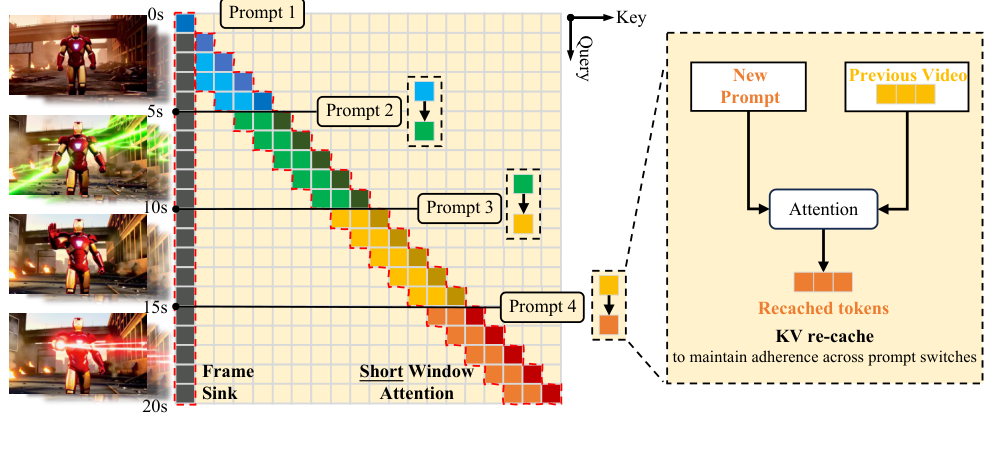
\includegraphics[keepaspectratio,alt={短窗口、历史锚点与提示切换时的缓存刷新 （论文示意，来源：longlive）}]{assets/seedance/figures/streaming-cache.png}}
\caption{短窗口、历史锚点与提示切换时的缓存刷新 （论文示意，来源：longlive）}
\end{figure}

图中短窗口控制近期历史的计算量，早期锚点提供身份和场景线索；提示变化后，则用历史画面与新提示重新建立缓存。它们分别作用于成本、保持和条件更新，需要与同一套训练及推理依赖对应。

但早期锚点也不能代替全部事件状态。人物后来拿起钥匙，开头没有这件事，继续读开头仍然不知道钥匙现在在哪里。于是还需要近期事件或主体状态的记忆，窗口大小和剧情记忆不能当成同一个参数。

\section{怎样验证缓存和长程记忆}\label{seedance-m06-ux600eux6837ux9a8cux8bc1ux7f13ux5b58ux548cux957fux7a0bux8bb0ux5fc6}

先以不使用缓存的完整重算结果为基线，在相同噪声下逐层比较输出；再分别改变提示、参考、历史和时间条件，确认系统会使相应缓存失效。修改过去片段时，因果模型的该片段及后续缓存通常需要刷新，双向场景模型甚至可能影响整场景。

长程效果再按时间分段看。可将生成长度扩到训练长度的两倍、四倍，记录各段身份、道具、背景与动作错误，同时单独观察新提示多久生效。只给整段一个平均分，后半段崩坏可能被前半段掩盖。缓存与这些保持问题都确认后，再继续调窗口、精度和吞吐。

\section{从极简代码到真实实现}\label{seedance-m06-ux4eceux6781ux7b80ux4ee3ux7801ux5230ux771fux5b9eux5b9eux73b0}

缓存首先是依赖版本问题。提示、历史、噪声策略或模型改变时，旧状态就不能继续当成相同条件：

\begin{verbatim}
key = hash_of(model, prompt, references, history, noise_policy)
if key != previous_key:
    cached_layers.clear()
\end{verbatim}

\hyperref[code-cache-context]{cache\_context.py} 只说明失效机制，没有实现完整自回归 attention。真实的缓存写入、当前块去噪和窗口读取，直接看 \href{https://github.com/NVlabs/LongLive/blob/31c70d9071cd7851d82939806dc9fac645fcabe5/LongLive1.0/pipeline/causal_inference.py}{LongLive1.0 因果推理} 与 \href{https://github.com/NVlabs/LongLive/blob/31c70d9071cd7851d82939806dc9fac645fcabe5/LongLive1.0/wan/modules/causal_model.py}{CausalWanSelfAttention}。普通双向模型无法只靠添加这个字典获得相同能力。

% Imported from topics/video-generation/seedance-2.5/long-video-spec.md
\chapter{长视频执行与因果缓存协议}\label{seedance-m24}
\moduleinfo{M24}{候选设计与工程选型；组合效果待验证}{\hyperref[src-long-context-tuning]{\texttt{long-context-tuning}}、\hyperref[src-longlive]{\texttt{longlive}}、\hyperref[src-longlive-code]{\texttt{longlive-code}}、\hyperref[src-ltx-2]{\texttt{ltx-2}}、\hyperref[src-ltx-original-code]{\texttt{ltx-original-code}}、\hyperref[src-ltx-original-model]{\texttt{ltx-original-model}}}

上一章明确了缓存成立的条件，这里把联合长片与因果续写分别写成候选执行过程。

长视频到这里分成两条计算图。一次联合生成时，未来镜头可反过来约束前面；逐块续写时，已交付历史却不能再依赖未来带噪状态。因此两者不只是请求长度不同，注意力、训练历史与缓存都要按这种依赖重新定义。

候选路线先训练联合长片，再派生块间因果版本。长上下文调优和流式方法提供可借鉴机制，但音视频联合迁移与训练尚未完成。下面先把需要满足的关系写清楚。

\section{共同的镜头状态是什么}\label{seedance-m24-ux5171ux540cux7684ux955cux5934ux72b6ux6001ux662fux4ec0ux4e48}

每个场景保存全局角色与环境描述，每个镜头保存局部事件、相机与时间范围；额外记录角色位置、服装、道具归属、已发生事件和待发生事件。

状态也有确定程度：用户指定、画面观察和模型推断分别记录证据时间与置信度。比如计划写钥匙在 A 手里，实际生成却已掉落，不能继续把计划当作发生事实；应重做结果或修正状态，再生成后续。

状态文本能帮助检索条件，却替代不了人物外观、动作和几何。新镜头仍要同时读取身份参考、相关关键帧和近期事件证据。若只把摘要越写越长，可能文字完整了，视觉条件仍然缺失。

\section{联合长片保留全局连接}\label{seedance-m24-ux8054ux5408ux957fux7247ux4fddux7559ux5168ux5c40ux8fdeux63a5}

第一版按8、16、30秒课程训练，视频与音频的token时间来自相同媒体时钟。每个样本使用全局条件和shot局部条件，新支路根据镜头与时间读取参考。

初始全段共享sigma，随后单列异步镜头任务。异步任务为每个镜头采样 \(\sigma_s\)，镜头覆盖内的视频和音频使用匹配的噪声状态；跨镜头边界token单列归属规则，不能同一token同时写两个sigma。

每个 token 的噪声状态也要真实传给模型。干净镜头为 0，活动镜头随步数变化；如果输入已异步，调制仍广播全局 sigma，两者就在描述不同状态。联合版本每步重算两条动态流，暂不把跨步历史 KV 当作精确值。

\section{因果版本如何分块}\label{seedance-m24-ux56e0ux679cux7248ux672cux5982ux4f55ux5206ux5757}

时间块目标约4秒，实际边界根据codec网格生成。视频与音频token各自保存位置网格区间，使用共同时间边界分配block ID；跨边界token延后归入能够完整容纳其区间终点的块，边界形成一个可报告的缓冲区。

时间网格还不是完整感受野。某个 token 的编码或预处理若读取未来，就要按真实依赖终点延后入块，或改用匹配的因果处理。只修改 block ID，没有消除编码阶段已经发生的信息泄漏。

因此按真实区间分块，比直接拿 token 下标除固定长度更清楚。训练推理用同一映射，RoPE 保留全局坐标；不能每次续写都将活动块当成新首帧，也不能把独立编码的局部首帧规则当作全局连续编码。

令query与key的块编号分别为 \(b_q,b_k\)：

\[
\operatorname{allow}(q,k)=\mathbf1[b_k\le b_q].
\]

同块内部双向，跨块只读过去，这条规则同时适用于视频 self、音频 self、视频读音频和音频读视频。若只改视频自身，未来仍可先进入声音，再从 AV 路径回来，因果约束并没有成立。

极简布尔关系见 \hyperref[code-block-causal-mask]{block\_causal\_mask.py}。真实长序列应使用块稀疏表示；该示例构造稠密布尔矩阵，只便于看清方向。

\section{原生前向接口还需要补什么}\label{seedance-m24-ux539fux751fux524dux5411ux63a5ux53e3ux8fd8ux9700ux8981ux8865ux4ec0ux4e48}

原Attention层支持mask参数，但原联合块的self与AV调用没有透传完整的候选因果mask。需要给 \codepath{TransformerArgs} 或额外执行上下文增加四类mask，并逐调用传入相应kernel。

其它支路也沿依赖检查：源条件塔、历史池化、字幕与对白能看到什么？用户预先给完整剧情或固定音轨，是已知任务条件；读取尚未生成的真实未来视频，则改变了预测问题。两者都叫“未来信息”会掩盖关键区别。

历史token噪声时间固定为0，当前块按采样sigma变化。跨模态调制使用各自token的噪声状态，避免把当前块的全局sigma广播进已缓存历史。

\section{缓存写入必须等到干净历史成立}\label{seedance-m24-ux7f13ux5b58ux5199ux5165ux5fc5ux987bux7b49ux5230ux5e72ux51c0ux5386ux53f2ux6210ux7acb}

第 \(k\) 块采样结束后，它成为下一块的干净条件。最后一个带噪步生成的隐藏状态仍属于那个带噪输入，不能直接写为永久历史缓存。

\begin{verbatim}
1. 用已有干净历史和当前噪声块完成当前块采样。
2. 固定生成结果、全局坐标与已确认状态，当前块sigma设为0。
3. 以同一因果执行图重新计算当前块的干净隐藏状态。
4. 写入各层流内与AV读取需要的K/V，提交历史版本。
5. 下一个块每步只计算活动块，并读取已提交历史。
\end{verbatim}

每层至少区分视频self、音频self、音频作为视频条件、视频作为音频条件四套K/V。它们有不同投影与调制，不能把一个名为 \codepath{history_kv} 的张量供所有模块共用。

历史只能读更早历史和固定条件，不读当前未来目标。这样同一份历史 K/V 对所有活动去噪步才保持不变，缓存的等价性有了计算图依据，而不只是实现里存下了一个张量。

\section{提示改变时怎样失效}\label{seedance-m24-ux63d0ux793aux6539ux53d8ux65f6ux600eux6837ux5931ux6548}

缓存键包括模型与适配器、历史内容、坐标、噪声策略、文本条件、参考、结构条件和状态版本。一个历史层若读取了新变化的条件，其K/V就需要刷新；不能仅按原始视频哈希命中。

首版可先保守处理：编辑历史或改变全局条件，就重建受影响前缀与后续。若希望新提示只作用未来，必须固定历史写入时所用条件，将新提示单独送给活动块，并在训练中使用同样规则。这是另一种明确的执行含义，不能靠缓存命中自动获得。

窗口还有一个容易漏掉的关系。旧 token 已被淘汰，保留的隐藏状态却可能早已读过它。因此按相同窗口策略逐步重放，和只拿当前窗口从头算一次，不一定相等。先用完整历史定义正确性，再独立比较有限窗口的收益和退化，才知道省掉了什么。

\section{自生成历史不能直接接任意真实未来}\label{seedance-m24-ux81eaux751fux6210ux5386ux53f2ux4e0dux80fdux76f4ux63a5ux63a5ux4efbux610fux771fux5b9eux672aux6765}

训练历史先从真实数据开始，再加入接近模型失真的受控扰动，最后才逐步使用学生自己生成的历史。每一步都在改变当前块所面对的条件分布，需要分别观察。

例如学生已生成钥匙掉落，原片后续却假设钥匙仍在手里，这时直接接原真实未来，监督就与条件冲突。可以让固定 teacher 在同一历史、参考和下一事件条件下重新标后续，再滤掉矛盾与严重错误；也可采用对齐的短 rollout 蒸馏。首版选前一项，因此 teacher 数据生成也要计入预算。

历史停止反传，当前块计算flow损失。逐步把自生成历史比例从30\%提高到70\%只是课程起点；若teacher重标质量不够，先维持真实/扰动历史，不把任意学生历史与真实未来拼成``可训练对''。

\section{解码与交付也有因果性}\label{seedance-m24-ux89e3ux7801ux4e0eux4ea4ux4ed8ux4e5fux6709ux56e0ux679cux6027}

再往输出端看，Transformer 能缓存，不等于 decoder 已经零前瞻。视频解码器可能读后续 latent，音频 vocoder 也有上下文和缓冲，所以“模型逐块生成”尚不能直接推出“帧可以立刻提交”。

首版先离线逐块生成、整段解码。若要在线输出，就另定义解码 halo 与前瞻，等需要的上下文到齐再提交；若要求完全无前瞻，则要相应因果 codec 及训练。KV-cache 本身没有改变解码器的未来依赖。

\section{长片验收按时间段展开}\label{seedance-m24-ux957fux7247ux9a8cux6536ux6309ux65f6ux95f4ux6bb5ux5c55ux5f00}

分别检查前段、中段和末段的身份、运动、道具状态、事件顺序与声画同步。联合三十秒、块式续写到更长时长、多镜头返回同场景，是三组不同任务。

缓存正确性先比较相同因果执行图的完整重算与缓存结果，再比较窗口和量化版本。真实实现可读 \href{https://github.com/NVlabs/LongLive/blob/31c70d9071cd7851d82939806dc9fac645fcabe5/LongLive1.0/pipeline/causal_inference.py}{LongLive因果推理}，LTX迁移入口为 \href{https://github.com/Lightricks/LTX-2/blob/bd92a5f408eb8c99f8c05e9fe2fcaaec8b56b638/packages/ltx-core/src/ltx_core/model/transformer/transformer.py}{联合块} 与 \href{https://github.com/Lightricks/LTX-2/blob/bd92a5f408eb8c99f8c05e9fe2fcaaec8b56b638/packages/ltx-core/src/ltx_core/model/transformer/attention.py}{Attention}。后者尚需上述因果化改动。

% Imported from topics/video-generation/seedance-2.5/integrated-design.md
\chapter{完整联合音视频候选架构}\label{seedance-m19}
\moduleinfo{M19}{候选设计与工程选型；组合效果待验证}{\hyperref[src-ltx-2]{\texttt{ltx-2}}、\hyperref[src-alchemint]{\texttt{alchemint}}、\hyperref[src-vace]{\texttt{vace}}、\hyperref[src-videocof]{\texttt{videocof}}、\hyperref[src-vincie-next]{\texttt{vincie-next}}、\hyperref[src-geometry-as-context]{\texttt{geometry-as-context}}、\hyperref[src-long-context-tuning]{\texttt{long-context-tuning}}、\hyperref[src-longlive]{\texttt{longlive}}、\hyperref[src-ltx-original-code]{\texttt{ltx-original-code}}、\hyperref[src-vace-code]{\texttt{vace-code}}、\hyperref[src-videocof-code]{\texttt{videocof-code}}、\hyperref[src-ltx-original-model]{\texttt{ltx-original-model}}}

至此各条输入和执行路径已有定义，下面将它们放回共同主干，检查完整候选系统是否相互兼容。

各模块已有了局部定义，现在把问题收回来：同一系统要读图片、视频、音频与结构条件，生成较长音视频，再定向修改，怎样形成一条可以训练的计算链？必须先选共同表示和主干，让时间、条件与目标在各处使用同样的含义。仅列出多篇方法的名称，还没有建立这种关系。

下面选定 LTX-2 初始公开系列的非蒸馏联合音视频模型作为共同主干，保留其 VAE、文本组件、双流 block 和原生 scheduler，再新增有绑定的参考记忆、源视频条件、区域定位与结构控制。它是面向类似公开能力的\textbf{完整候选设计}；尚未训练验证，也不代表 Seedance 2.5 的真实内部实现或同等效果。

\section{明确哪些保留，哪些新增}\label{seedance-m19-ux660eux786eux54eaux4e9bux4fddux7559ux54eaux4e9bux65b0ux589e}

{\def\LTcaptype{table} % do not increment counter
\small\setlength{\tabcolsep}{3pt}\renewcommand{\arraystretch}{1.18}
\begin{longtable}[]{@{}
  >{\raggedright\arraybackslash}p{(\linewidth - 4\tabcolsep) * \real{0.1900}}
  >{\raggedright\arraybackslash}p{(\linewidth - 4\tabcolsep) * \real{0.3900}}
  >{\raggedright\arraybackslash}p{(\linewidth - 4\tabcolsep) * \real{0.4200}}@{}}
\toprule\noalign{}
\begin{minipage}[b]{\linewidth}\raggedright
层级
\end{minipage} & \begin{minipage}[b]{\linewidth}\raggedright
选定设计
\end{minipage} & \begin{minipage}[b]{\linewidth}\raggedright
状态
\end{minipage} \\
\midrule\noalign{}
\endhead
\bottomrule\noalign{}
\endlastfoot
视频表示 & 原生视频 VAE，128通道，时间/8、空间/32 & 沿用共同基座 \\
音频表示 & 原生音频 VAE，约25个时间 token/秒、每时间位置128维 & 沿用共同基座 \\
文本 & 对应模型的冻结文本编码器、特征投影与连接器 & 必须匹配原系列 \\
生成主干 & 14B视频流＋5B音频流、原生跨模态交换 & 沿用联合建模方向 \\
参考记忆 & 独立素材编码、角色/类型/时间绑定、定额池化、门控读取 & 需要新增和训练 \\
源条件 & 待变/保留条件拆分、mask投影、残差 adapter & 需要新增和训练 \\
区域定位 & 自动区域预测或人工mask；可选编辑示例图 & 需要数据和新增任务 \\
空间控制 & 白模/depth/pose/camera条件与关键视角记忆 & 先实现已知结构路径 \\
长续写 & 从联合模型另派生因果块模型 & 单独训练，不是推理开关 \\
\end{longtable}
}

早期 Wan-1.3B 路线继续用于低成本阅读、机制和单能力实验；完整联合设计不把它的 latent 或权重接入 LTX。LTX 后续型号也不自动与这套原系列接口相同，实际工程以固定版本与模型配置配套。

共同基座具体选为原系列19B开发权重：48个联合块，视频宽4096、音频宽2048，split RoPE。新增模块位于第4、8直至48块之后，每处依次接源/结构残差、视觉参考和声音参考；参考支路内宽512，投影与门控逐处独立。完整维度、共享规则与参数保存方式见 \hyperref[seedance-m21]{模块契约}，不能仅凭原生构造器默认值替代实际权重配置。

\section{统一任务规格}\label{seedance-m19-ux7edfux4e00ux4efbux52a1ux89c4ux683c}

因此先把请求翻译成任务对象：时长、帧率、镜头计划、角色与 speaker、参考绑定、源视频、编辑范围、结构条件、音轨保持、种子和质量档位。后续每个模块都从这个对象取得自己的条件，不再独立猜一次用户要求。

\begin{verbatim}
用户要求
  → 任务编译与素材登记
  → 独立编码：文本 / 参考视觉 / 参考音频 / 源条件 / 结构
  → 按镜头和时间建立条件可见性
  → 联合视频与音频去噪
  → 解码、合法时长裁切、局部合成与音轨保持
  → 分项检查、定向返工或交付
\end{verbatim}

例如三十秒广告包含两个镜头：角色A前半段展示产品，后半段角色B加入；产品图只锁结构，动作视频只锁手部动作，声音参考只锁speaker A。若第二镜头的外套颜色错误，编辑请求保留角色、产品、动作和音轨，只重做指定区间的外套区域。

提示改写后，这些绑定仍要在。保留原始指令和编译结果，才能检查目标有没有被改变。一段更长的提示可以增加描述，却不能代替角色、素材和区间之间明确的对应。

条件还注明是用户给定、自动估计还是模型生成。自动区域低置信时先确认区域，主体冲突时先修绑定；结果若只错了某个镜头或局部，就沿该范围重做。身份、动作、台词、保持与返工最后按交付任务统计，而不是只留下最好的一次候选。

\section{共同潜空间与时间对齐}\label{seedance-m19-ux5171ux540cux6f5cux7a7aux95f4ux4e0eux65f6ux95f4ux5bf9ux9f50}

视频经原 VAE 得到：

\[
z_v\in\mathbb{R}^{B\times128\times T_v\times H_v\times W_v},
\quad T_v=1+(F-1)/8,\quad H_v=H/32,\ W_v=W/32.
\]

音频实现可保留 \codepath{B,8,Ta,16} 的 codec 布局，进入主干时每个时间位置整理为128维。音频约25个时间位置/秒；视频与音频仍通过物理时间而非索引一一对应。所有特征继承原模型归一化，不能为统一 shape 任意换 codec。

以三十秒、24fps为例，最终要720帧。为了满足 \(1+8k\) 的编码约束，可在模型内部使用721帧，输出裁为720帧，并保存补帧映射；音频严格保留三十秒。训练的padding有效位和像素监督不得把额外帧当成真实动作。latent边界覆盖多个像素帧，不能仅把最后一个latent粗暴置为无效。

\section{参考记忆的两条读取支路}\label{seedance-m19-ux53c2ux8003ux8bb0ux5fc6ux7684ux4e24ux6761ux8bfbux53d6ux652fux8def}

图片与视频进入视觉参考记忆，音频进入音频参考记忆，分别保存来源、主体、角色、时间、置信度与有效位。首版视觉预算2048、音频预算512；按每图32、每视频64、每音频32摘要token，30/10/10份素材在文件容量上可被表示，但质量必须逐级验证。

参考支路安插在每四个原生block后作为初始设计。先门控读取图像/外观与声音信息：

\[
\Delta h_v=g_v\operatorname{Attn}(Q_v,K_{r_v},V_{r_v};B_v),
\qquad
\Delta h_a=g_a\operatorname{Attn}(Q_a,K_{r_a},V_{r_a};B_a).
\]

新增支路先按镜头屏蔽不允许的主体，按时间加软偏置，并保留 null token。空间 query 本身没有 subject ID，只有已给布局、源跟踪或可靠预测区域时，才有依据作空间硬约束；其余绑定通过主体 embedding 与训练学习。两条流再经原生 AV 模块交换信息，声音也要遵守角色与 speaker 的映射，不能把归属全部留给 attention 去猜。

动作视频中的姿态、光流和相机走结构支路，需要时关闭原人物外观。音色克隆则用同 speaker 跨台词配对。于是“能输入声音”与“能保持指定音色”仍隔着相应的条件和监督，不能由接口存在推出能力已经学到。

需要保留对白或配乐时，完整干净音轨走对齐条件路径，不能压成32个音色摘要后期待逐字或逐拍一致。其时序token按原音频codec单独计费；多人同时说话时，混合音频token可能对应多个speaker，不能无条件强制一个token只绑定一个人。

\section{源条件与区域预测怎样接入}\label{seedance-m19-ux6e90ux6761ux4ef6ux4e0eux533aux57dfux9884ux6d4bux600eux6837ux63a5ux5165}

源视频再拆成待变、保留内容与 mask，分别对齐编码后进入 context adapter。带噪目标仍从原主干输入，新增支路在约定层加残差。参考图、源图和源视频独立编码，避免在 VAE 时间轴上制造本来不存在的连续关系。

用户没给 mask 时，先用 grounding、分割或训练得到的视觉区域预测定位；关键帧编辑对再提供原样到目标外观的对应。首版先把定位与生成分开，便于检查，不将源、区域与目标一开始全部堆进大序列。

这里干净源条件与目标覆盖又要分清。源条件不随目标去噪时间变化；目标的已知区若作重噪覆盖，则仍沿一条固定噪声路径变化。训练必须选明这种条件方式，否则同名输入在两处使用不同时间含义。

\section{原生双流块怎样保持同步}\label{seedance-m19-ux539fux751fux53ccux6d41ux5757ux600eux6837ux4fddux6301ux540cux6b65}

每个流保留自身self-attention、文本cross-attention、双向音视频cross-attention和FFN。流内视觉使用时空位置，跨模态Q/K只使用共同物理时间；对方的噪声状态通过调制与门控影响交换强度。

\begin{figure}
\centering
\pandocbounded{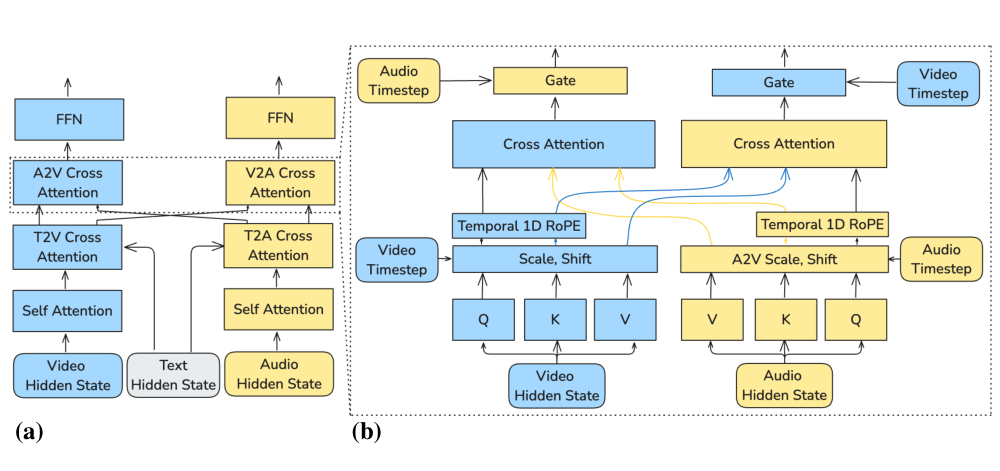
\includegraphics[keepaspectratio,alt={联合主干与音视频跨注意力的组成 （论文示意，来源：ltx-2）}]{assets/seedance/figures/joint-av-block.png}}
\caption{联合主干与音视频跨注意力的组成 （论文示意，来源：ltx-2）}
\end{figure}

交换时两边先读取同一组旧状态，再各自加残差。若先更新一边再给另一边读，执行顺序本身就改变了计算图。缺音轨时跳过无效目标和交互，真实静音仍监督；需要保留原音轨时，则把它作干净条件，输出复用，不为“联合”强行重生声音。

\section{一次采样的具体执行顺序}\label{seedance-m19-ux4e00ux6b21ux91c7ux6837ux7684ux5177ux4f53ux6267ux884cux987aux5e8f}

采样前可先缓存固定条件编码，再按任务决定哪些目标更新。可读条件、去噪更新、损失有效位和最终替换范围各有一个 mask：它们来自同一请求，但对应不同计算，因而分别保存。

{\def\LTcaptype{table} % do not increment counter
\small\setlength{\tabcolsep}{3pt}\renewcommand{\arraystretch}{1.18}
\begin{longtable}[]{@{}
  >{\raggedright\arraybackslash}p{(\linewidth - 6\tabcolsep) * \real{0.1600}}
  >{\raggedright\arraybackslash}p{(\linewidth - 6\tabcolsep) * \real{0.2800}}
  >{\raggedright\arraybackslash}p{(\linewidth - 6\tabcolsep) * \real{0.2800}}
  >{\raggedright\arraybackslash}p{(\linewidth - 6\tabcolsep) * \real{0.2800}}@{}}
\toprule\noalign{}
\begin{minipage}[b]{\linewidth}\raggedright
任务
\end{minipage} & \begin{minipage}[b]{\linewidth}\raggedright
视频状态
\end{minipage} & \begin{minipage}[b]{\linewidth}\raggedright
音频状态
\end{minipage} & \begin{minipage}[b]{\linewidth}\raggedright
模型更新与交付
\end{minipage} \\
\midrule\noalign{}
\endhead
\bottomrule\noalign{}
\endlastfoot
文本/参考生成音视频 & 带噪目标 & 带噪目标 & 联合更新与解码 \\
仅有视频监督 & 带噪目标 & 缺失标记 & 只更新视频，屏蔽无效AV连接 \\
保留源音轨的视觉编辑 & 带噪目标＋干净源视觉条件 & 干净源音频条件 & 只更新视频，交付复用原音轨 \\
因果续写 & 干净历史＋当前带噪块 & 干净历史＋当前带噪块 & 仅更新当前块，两流遵守相同历史边界 \\
\end{longtable}
}

保留音轨与缺音轨是新增任务策略，训练必须出现相同状态，不能只在推理时把音频噪声改成零。干净音频仍可提供口型条件，缺音轨则完全不提供有效声音信息。

还需把模态存在、隐藏计算和 latent 更新分开。保留声音时，输入音频 latent 固定且干净，不计算音频 loss，也不更新它；声音流仍参与 AV 计算。其深层状态一旦读取当步视频，就仍随步数变化，所以默认只缓存 codec 结果，Transformer 声音特征每步重算。

\begin{verbatim}
1. 编译任务，确定内部帧数、补帧映射、两流时间坐标和各类mask。
2. 独立编码参考、源内容和结构；按模型/内容/变换版本缓存。
3. 未给区域时先定位；确定区域后编码待变/保留条件。
4. 活动目标从噪声起步，沿版本固定的sigma序列调用联合主干和新增支路。
5. 每步只更新活动目标；可选已知区重噪覆盖使用同一固定噪声路径。
6. 解码并按媒体时钟裁切；源像素与源音轨按交付规则直接合成。
7. 检查目标变化、外区保持、声画同步和角色状态，定向返回失败步骤。
\end{verbatim}

新增参考strength首先作为门控残差的缩放量，独立于原生guidance保存。短片保留原生采样配置作对照，长片候选采用有界长度shift并与训练噪声课程配套；这是需要比较的新选择，见 \hyperref[seedance-m25]{数据与训练规格}。具体步数从配套配置读取；尚未进行少步数训练时，不指定一个未经验证的高速档位。

\seedancenetworkfigure{5}{Seedance 2.5 推测方案的联合采样回路与两种长视频执行关系。图中主干沿用总览章的 Dual-MMDiT 推测；本章 LTX 替代实现说明同类执行接口，不表示二者逐层拓扑相同。}{fig:seedance-joint-inference}

\section{联合长片与因果续写分别保存版本}\label{seedance-m19-ux8054ux5408ux957fux7247ux4e0eux56e0ux679cux7eedux5199ux5206ux522bux4fddux5b58ux7248ux672c}

第一版先保留整段联合去噪，按 8、16、30 秒任务逐步训练，全局连接作质量对照。因为视频和声音状态每步都变，这一版不使用跨步历史 KV 来声称精确复用。先看长程条件是否真的保持，再改依赖结构。

续写模型从它另行派生：以约4秒的时间块为单位，块内双向，块间只能读历史；视频和音频都采用同一块时间边界，四类流内与跨模态注意力都不能偷读未来。编码依赖越过边界的token延迟入块。训练先以真实/扰动历史起步，自生成历史需由teacher按实际历史重标后续并过滤状态冲突，历史梯度截断。

缓存的是在固定提示/参考/坐标/零噪声历史条件下生成的层状态。每块采样结束后须按干净历史重算再写入，不能提交最后一个带噪步的K/V。每次提示或过去内容改变，对相应依赖全量重建为正确性基线。原decoder并非无前瞻流式设计，首版整段解码交付；完整协议见 \hyperref[seedance-m24]{长视频执行规格}。训练未完成前，可用尾段重叠条件做续写，但应如实记为``条件续写''，不能宣称已获得实时AR缓存能力。

\section{白模与长程空间记忆}\label{seedance-m19-ux767dux6a21ux4e0eux957fux7a0bux7a7aux95f4ux8bb0ux5fc6}

已知白模先渲染同步depth/normal/pose/camera射线，经过type专用投影与context adapter进入视频流。静态结构、动态主体状态、带置信度的关键视角分开保存，每镜头检索少量可见且相关的历史视图。

首版不要求同时恢复完整世界，生成图像的深度也不作为精确几何真值。已知 CAD 给定的约束与后续学习型几何预测，来源和确定程度不同，应分别监督。

\section{三十秒的成本必须先算清楚}\label{seedance-m19-ux4e09ux5341ux79d2ux7684ux6210ux672cux5fc5ux987bux5148ux7b97ux6e05ux695a}

取内部721帧、\(512\times896\)分辨率，无额外空间patch时：

\[
N_v=91\times16\times28=40\,768,\qquad N_a\approx750.
\]

视频dense attention每头约有16.6亿个连接；单方向音视频交互约3060万个；2048视觉参考的完整交叉读取约8350万个。Flash attention避免显式保存完整矩阵，却不会消除算术量。

这也解释了从短片、小分辨率和少量参考开始的原因。扩到 30 秒后，显存分片、context parallel、条件预算与训练课程都要跟上。窗口、稀疏和少步数可再优化，但需要质量对照，不能预先作为无损能力计入。

\section{方案的完成边界}\label{seedance-m19-ux65b9ux6848ux7684ux5b8cux6210ux8fb9ux754c}

到这里，共同主干、表示、条件路径、训练任务，以及两种长视频方式，已经有了对应关系，可以逐块实施。仍待实验回答的是：压缩参考后细节是否足够，复杂动作能否稳定到三十秒，音色与局部保持能否达到要求，以及训练要花多少资源。这些不能由结构图本身推出。

真实联合音视频与训练从 \href{https://github.com/Lightricks/LTX-2}{LTX-2} 进入；统一视觉条件借鉴 \href{https://github.com/ali-vilab/VACE}{VACE}，区域定位式编辑看 \href{https://github.com/knightyxp/VideoCoF}{VideoCoF}，因果流式机制看 \href{https://github.com/NVlabs/LongLive}{LongLive}。迁移这些机制仍是新增工作，不是现成仓库之间的一键连接。

可逐项审阅的 \href{https://github.com/foocker/multimodal-journey/blob/0f1b6bb86d609d75d8c2582063d85707d0180d39/topics/video-generation/seedance-2.5/design-spec.json}{设计规格} 保存形状、预算、依赖与训练候选值；已固定checkpoint的revision、文件名和远端声明哈希，并读取配置与文件头，张量载荷尚未下载，本地完整校验哈希为空。完整训练课程另见 \hyperref[seedance-m20]{联合训练配方}，资源与返工口径见 \hyperref[seedance-m26]{推理与交付规格}。

\part{数据、训练与后训练}
% Imported from datasets/recipes/audio-video-production/README.md
\chapter{M11 训练数据的制作与隔离}\label{seedance-m11}
\moduleinfo{M11}{基础方法与机制解释}{\hyperref[src-seedance-1.0]{\texttt{seedance-1.0}}、\hyperref[src-tarsier2]{\texttt{tarsier2}}、\hyperref[src-phantom]{\texttt{phantom}}、\hyperref[src-vincie]{\texttt{vincie}}、\hyperref[src-long-context-tuning]{\texttt{long-context-tuning}}、\hyperref[src-tarsier-code]{\texttt{tarsier-code}}、\hyperref[src-diffsynth-code]{\texttt{diffsynth-code}}、\hyperref[src-vincie-code]{\texttt{vincie-code}}}


视频训练数据不是一个``视频文件加一句描述''的目录。参考控制需要知道素材属于哪个主体，局部编辑需要知道允许改变的范围，续写需要知道哪些帧已经发生。数据制作的目标，是把这些约束变成可重复执行、可追踪来源的样本。

\section{先定义样本，再决定收什么}\label{seedance-m11-ux5148ux5b9aux4e49ux6837ux672cux518dux51b3ux5b9aux6536ux4ec0ux4e48}

一个训练样本应围绕一个目标任务组织，包含目标片段、条件、文字描述、参考绑定和有效监督位置。原始长视频、场景和主体属于上层来源信息，可以派生多个样本，但不能在拆分后丢失它们的关联。

{\def\LTcaptype{table} % do not increment counter
\small\setlength{\tabcolsep}{3pt}\renewcommand{\arraystretch}{1.18}
\begin{longtable}[]{@{}
  >{\raggedright\arraybackslash}p{(\linewidth - 4\tabcolsep) * \real{0.1900}}
  >{\raggedright\arraybackslash}p{(\linewidth - 4\tabcolsep) * \real{0.3900}}
  >{\raggedright\arraybackslash}p{(\linewidth - 4\tabcolsep) * \real{0.4200}}@{}}
\toprule\noalign{}
\begin{minipage}[b]{\linewidth}\raggedright
任务
\end{minipage} & \begin{minipage}[b]{\linewidth}\raggedright
条件
\end{minipage} & \begin{minipage}[b]{\linewidth}\raggedright
目标与关键标签
\end{minipage} \\
\midrule\noalign{}
\endhead
\bottomrule\noalign{}
\endlastfoot
文本生成视频 & 动作与场景描述 & 目标片段、事件顺序 \\
主体参考 & 参考图与动作要求 & 同主体目标、角色绑定、允许变化属性 \\
局部编辑 & 源片段、指令、时间与空间 mask & 编辑后片段、保持项与变化项 \\
续写 & 历史片段、新事件要求 & 后续片段、历史截止时间 \\
\end{longtable}
}

如果评测未见身份，训练与测试需要身份隔离；如果只评同身份的新场景，则应按场景和原始来源隔离。二者回答不同问题，不能混成一个泛化结论。

\section{原始素材入库需要保留什么}\label{seedance-m11-ux539fux59cbux7d20ux6750ux5165ux5e93ux9700ux8981ux4fddux7559ux4ec0ux4e48}

每份媒体保存内容哈希、来源、版本、训练与再分发使用范围，以及容器、codec、分辨率、帧率和时间戳信息。参考素材、编辑源和目标媒体应各有记录，不能只批准目标文件。

视频还可能包含旋转、HDR 色彩、可变帧率和音频偏移。预处理必须保存这些信息及对应变换：真正重采样音频，真正调整视频帧序列，并保留原时间戳到新帧索引的映射。缓存可按``原文件哈希、变换配置、工具版本''确定，任何一项改变都产生新版本。

\section{切镜、过滤与去重怎样衔接}\label{seedance-m11-ux5207ux955cux8fc7ux6ee4ux4e0eux53bbux91cdux600eux6837ux8854ux63a5}

自然切镜检测适合把长视频拆成可处理片段，但闪光、快速运动和淡入淡出容易误判，必须抽检。质量标签应分别记录压缩损伤、失焦、遮挡字幕、过暗、静止、异常加速和声画错位，避免一个总分掩盖可修复的问题。

\begin{figure}
\centering
\pandocbounded{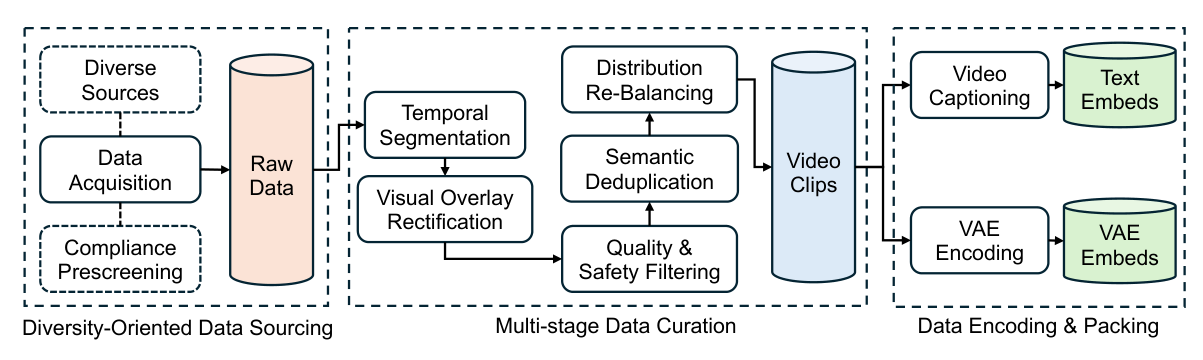
\includegraphics[keepaspectratio,alt={从多来源视频整理到描述与潜变量打包 （论文示意，来源：seedance-1.0）}]{assets/seedance/figures/data-pipeline.png}}
\caption{从多来源视频整理到描述与潜变量打包 （论文示意，来源：seedance-1.0）}
\end{figure}

缩放、裁剪和补帧时，框、mask、关键点与相机条件必须同步变换。如果模型要求 \(F=1+4k\)，补出的帧需要有效位标记，不能让它们像真实帧一样计入损失。

去重至少包含文件哈希、跨编码近重复和内容聚类。相邻镜头、同原片不同剪辑、共享参考和同主体关系会形成来源图；需要按关联分组划分训练、验证、测试，不能只随机打散 shot。

分布平衡也应在划分后处理：训练集可以提高长尾动作采样率，测试集则保留预先定义的分布。不断看测试结果再调采样或阈值，会让测试失去独立性。

\section{Caption 的工作是描述事实}\label{seedance-m11-caption-ux7684ux5de5ux4f5cux662fux63cfux8ff0ux4e8bux5b9e}

好的视频描述同时包含静态属性与动态事件：主体外观、环境、动作、物体状态、相机和可观测光照。事件应附时间范围，多镜头还要区分全局角色信息与镜头局部变化。

描述模型可以先由人工细粒度标注训练，再扩大自动描述规模。Tarsier2 采用 Qwen2-VL 初始化，并结合时间 grounding 和描述偏好优化；使用它做生成数据标注时，仍需检查是否漏事件、错顺序或编造动作。基础描述模型全参训练，与某个下游任务冻结视觉编码器，是两种不同设置。

Prompt 改写与 caption 生成也不同：前者把用户要求变成可用指令，后者从媒体提取事实。两者可以使用相近的结构，但改写器不能把``猫''改成``狗''，caption 模型也不能猜测画外台词和人物动机。

\section{参考、编辑与续写各有什么泄漏风险}\label{seedance-m11-ux53c2ux8003ux7f16ux8f91ux4e0eux7eedux5199ux5404ux6709ux4ec0ux4e48ux6cc4ux6f0fux98ceux9669}

主体参考若直接从目标帧截取，模型容易复制背景和姿态。跨片段同主体配对更适合学习身份保持，但相似特征并不证明身份相同，需要标签或人工核实。

编辑样本可以来自受控三维重渲染、真实人工编辑对或视频变化挖掘。前两类更容易提供明确真值，第三类应标为弱监督。相机、遮挡和光照一起变化时，不能只给一个``换颜色''标签。

续写样本必须记录历史截止时间，目标未来帧不得混入历史参考。已生成的训练轨迹也应与真实历史区分，因为模型在自生成历史上面对的误差分布不同。

\section{人工抽检怎样带动自动化}\label{seedance-m11-ux4ebaux5de5ux62bdux68c0ux600eux6837ux5e26ux52a8ux81eaux52a8ux5316}

可以先制作约 200 条分层试样，覆盖任务、运动幅度和主体数，并对至少一部分进行双人独立标注。这个数量是流程起点，不是充分数据规模。先建立争议样例的裁定规则，再扩大自动生成。

抽检分别统计事实准确率、关键事件召回、身份配对正确率、mask 越界和时间偏差。错误率高的类别增加抽样，已经稳定的类别才逐步降低人工比例。自动分数阈值需要用真实样本校准，不能从另一个数据集直接复制。

\section{编码与打包怎样支持重做}\label{seedance-m11-ux7f16ux7801ux4e0eux6253ux5305ux600eux6837ux652fux6301ux91cdux505a}

VAE 和文本编码器固定后，可以离线缓存潜变量与文本特征，但必须记录模型哈希、shape、dtype、缩放、后验采样方式和预处理。裁剪改变后复用旧 latent，会让媒体和条件悄悄错位。

按形状或 token 预算分桶可减少 padding。多个场景打包时，attention 应在场景边界隔离；缺音频、无效 padding、已知条件和生成目标分别设置有效位。

最终 manifest 保存每阶段输入、通过和淘汰数量，原因分布、split、来源分组、标注和变换版本。若一份素材撤回，应能追踪其派生 caption、latent、偏好对和训练运行。schema 校验可以发现字段、时间和已登记来源的冲突，媒体真实性、授权有效性与标注质量仍需真实处理与人工核查。

\section{真实工程从哪里进入}\label{seedance-m11-ux771fux5b9eux5de5ux7a0bux4eceux54eaux91ccux8fdbux5165}

批量描述入口可直接读 \href{https://github.com/bytedance/tarsier/blob/63de87a760c2aec6b31470a08046969a13787126/tasks/inference_caption.py}{Tarsier caption} 和 \href{https://github.com/bytedance/tarsier/blob/63de87a760c2aec6b31470a08046969a13787126/scripts/run_inference_caption.sh}{启动脚本}；训练数据如何进入模型可读 \href{https://github.com/modelscope/DiffSynth-Studio/blob/d32f72424cd22bc0ea8100cc57559149b4eac933/examples/wanvideo/model_training/train.py}{DiffSynth WanTrainingModule}。参考/编辑数据字段仍需按具体任务制作，不能把一个通用 caption CSV 自动解释为身份或局部保持监督。

% Imported from topics/video-generation/seedance-2.5/data-training-spec.md
\chapter{联合数据生产、噪声课程与参数组}\label{seedance-m25}
\moduleinfo{M25}{候选设计与工程选型；组合效果待验证}{\hyperref[src-ltx-2]{\texttt{ltx-2}}、\hyperref[src-ltx-original-code]{\texttt{ltx-original-code}}、\hyperref[src-tarsier2]{\texttt{tarsier2}}、\hyperref[src-tarsier-code]{\texttt{tarsier-code}}、\hyperref[src-alchemint]{\texttt{alchemint}}、\hyperref[src-vace]{\texttt{vace}}、\hyperref[src-videocof]{\texttt{videocof}}、\hyperref[src-longlive]{\texttt{longlive}}}

样本对象确定之后，继续写任务抽样、有效损失、参数组与恢复状态，明确一次更新到底包含什么。

条件已经分路以后，训练还要把它们重新接到同一损失和参数更新中。参考、编辑、几何与长叙事各有可行方法，并不表示样本一混合就能同时学好；它们的条件状态、监督有效位和梯度路径不同，也可能相互干扰，例如身份更稳但动作更静。

下面把这套联合主干的数据与更新过程写到可以检查的程度。任务比例、阈值和学习率是候选初值，用于开始实施与比较，不是已经测出的最优配方。

\section{数据生产分为八个可重做步骤}\label{seedance-m25-ux6570ux636eux751fux4ea7ux5206ux4e3aux516bux4e2aux53efux91cdux505aux6b65ux9aa4}

\begin{enumerate}
\def\labelenumi{\arabic{enumi}.}
\tightlist
\item
  媒体登记：内容哈希、来源组、可用范围、版本与音视频流信息。
\item
  时间规范化：真实重采样、PTS映射、声画偏移、色彩与旋转处理。
\item
  内容组织：镜头、场景、事件、人物与speaker候选。
\item
  关系确认：同主体跨片段配对、道具归属、speaker映射与资产家族。
\item
  来源划分：按共享主体/原片/三维资产关系确定开发、验证、测试分组。
\item
  任务派生：参考、动作、编辑、音频、几何和长叙事监督。
\item
  质量审阅：抽检与错误归因，剔除或回流重标。
\item
  编码打包：固定codec和文本特征，按形状/任务分桶，保存变换与编码版本。
\end{enumerate}

来源分组还会随新数据改变。若新参考把原来两个来源组连起来，就要重新检查 split；测试身份已经固定时，也不能把它的新视角加进训练，再继续声称身份隔离。去重关系因此需要随数据版本一起维护。

\section{每种自动工具输出什么}\label{seedance-m25-ux6bcfux79cdux81eaux52a8ux5de5ux5177ux8f93ux51faux4ec0ux4e48}

{\def\LTcaptype{table} % do not increment counter
\small\setlength{\tabcolsep}{3pt}\renewcommand{\arraystretch}{1.18}
\begin{longtable}[]{@{}
  >{\raggedright\arraybackslash}p{(\linewidth - 4\tabcolsep) * \real{0.1900}}
  >{\raggedright\arraybackslash}p{(\linewidth - 4\tabcolsep) * \real{0.3900}}
  >{\raggedright\arraybackslash}p{(\linewidth - 4\tabcolsep) * \real{0.4200}}@{}}
\toprule\noalign{}
\begin{minipage}[b]{\linewidth}\raggedright
环节
\end{minipage} & \begin{minipage}[b]{\linewidth}\raggedright
可选工具/来源
\end{minipage} & \begin{minipage}[b]{\linewidth}\raggedright
必须保存的结果
\end{minipage} \\
\midrule\noalign{}
\endhead
\bottomrule\noalign{}
\endlastfoot
媒体探测与转码 & ffprobe、FFmpeg & 原时间戳、变换参数、输出映射 \\
镜头与场景组织 & 场景检测器＋连续性审阅 & 切点、误切标记、场景组 \\
视频描述 & Tarsier/Tarsier2等 & 事实描述、事件时间、模型版本与人工纠错 \\
主体检测与跟踪 & Grounding DINO、SAM2等 & 框、逐帧mask、轨迹、可见性与置信度 \\
语音转录与分段 & ASR、diarization与必要的声源分离 & 台词、speaker段、重叠讲话和声画偏移 \\
结构条件 & 3D渲染器或深度/姿态/相机估计器 & 单位、坐标、有效位、估计置信度 \\
\end{longtable}
}

工具是候选生产组件，名称不代表已经安装或运行。阈值先在开发集按人工错误类型校准并登记版本；评估集上不再反复调阈值。

\section{八个数据池如何构造监督}\label{seedance-m25-ux516bux4e2aux6570ux636eux6c60ux5982ux4f55ux6784ux9020ux76d1ux7763}

{\def\LTcaptype{table} % do not increment counter
\small\setlength{\tabcolsep}{3pt}\renewcommand{\arraystretch}{1.18}
\begin{longtable}[]{@{}
  >{\raggedright\arraybackslash}p{(\linewidth - 4\tabcolsep) * \real{0.1900}}
  >{\raggedright\arraybackslash}p{(\linewidth - 4\tabcolsep) * \real{0.3900}}
  >{\raggedright\arraybackslash}p{(\linewidth - 4\tabcolsep) * \real{0.4200}}@{}}
\toprule\noalign{}
\begin{minipage}[b]{\linewidth}\raggedright
池
\end{minipage} & \begin{minipage}[b]{\linewidth}\raggedright
配对方式
\end{minipage} & \begin{minipage}[b]{\linewidth}\raggedright
不应混入的伪真值
\end{minipage} \\
\midrule\noalign{}
\endhead
\bottomrule\noalign{}
\endlastfoot
基础AV & 同一原片中的caption、视频和对齐音轨 & 猜测的画外台词、错位声音 \\
身份参考 & 同主体不同时间/视角参考与目标 & 只靠相似embedding认定身份 \\
动作/相机 & 目标提取结构，或同轨迹跨外观重渲染 & 用原人物外观暗中帮助控制 \\
声音参考 & 同speaker不同台词的干净语音与目标 & 背景音乐被标为音色 \\
区域编辑 & 人工编辑对、受控重渲染、明确标记的弱监督 & 把相机变化误标为单一颜色变化 \\
示例传播 & 源关键帧、编辑后关键帧与可靠目标视频 & 每帧独立图像编辑产生的闪烁``真值'' \\
几何控制 & 同资产与相机的控制层和目标材质渲染 & 米制渲染和未知尺度估计混用 \\
场景叙事 & 连续片段、镜头事件和角色道具状态 & 无关短片拼接成虚假连续场景 \\
\end{longtable}
}

难例也要主动收集：参考与目标相隔较远、同人换衣、中途缺席、动作换身份，以及 speaker 重叠。它们分别检验条件的不同含义。故意错绑参考的样本改用于冲突检测或比较，不继续拿原目标作普通 flow 真值。

先为每池制作一个分层审阅批次，例如200条、其中50条双人独立标注。这是流程校准数量。记录配对、时间、mask、caption和speaker各自错误率；没有足够真实样本时，减少解锁能力，而不是凭空补足池大小。

\section{样本有三个独立状态轴}\label{seedance-m25-ux6837ux672cux6709ux4e09ux4e2aux72ecux7acbux72b6ux6001ux8f74}

每个模态分别记录是否存在、是否算隐藏状态、是否更新 latent，每个目标再记录监督有效位。全局 batch 尽量按相同任务、形状和声音状态组织，是为了减少 padding 与分布式未使用参数的歧义，不是说所有样本天生使用同一损失。

\begin{verbatim}
基础AV：两流均存在、处理、更新，计算两流loss。
无音轨视频：只有视频目标；音频不存在，跳过声音与无效交互。
保留声音的编辑：音频存在且处理，但不更新latent、不计算音频loss。
局部对白编辑：活动声音区加噪并监督，外部为干净条件。
因果续写：历史为干净条件，只监督当前块，两流同一块划分。
\end{verbatim}

缺音轨没有声音目标，静音则有；保留声音又是另一种状态，它固定音频输出，却仍可能需要声音隐藏流提供口型条件。先区分这些变量，才能知道哪一项损失应当存在。

\section{噪声课程不能盲目按长序列外推}\label{seedance-m25-ux566aux58f0ux8bfeux7a0bux4e0dux80fdux76f2ux76eeux6309ux957fux5e8fux5217ux5916ux63a8}

原系列训练sampler使用长度相关的shifted logit-normal。它的偏移为：

\[
\mu(N)=0.95+\frac{1.10}{3072}(N-1024),
\qquad \sigma=\operatorname{sigmoid}(\xi+\mu(N)),\quad
\xi\sim\mathcal N(0,1).
\]

原实现按实际长度外推，并没有在4096处自动截断。当 \(N=40\,768\) 时，\(\mu\approx15.18\)，分布中位数接近0.9999997。长阶段照抄会高度集中在几乎纯噪声的位置，缺少足够的中低噪声训练。

候选长阶段采用：90\%有界shifted logit-normal、10\%均匀sigma；偏移限制在0.95至2.05之间。长度只计算目标视频token，不加参考摘要数；短片原生配置单独保留为对照。推理sigma调度也固定同一候选shift策略与原生端点处理，避免训练改了、验证仍使用另一套外推。

这个课程明确改变了原配方，所以必须保留原生对照，不能先叫作无损改进。基础 AV 两流共用 sigma，固定条件为 0，异步镜头另抽镜头 sigma；首版暂不增加没有依据的任意双流独立组合。

\section{损失先按样本有效元素平均}\label{seedance-m25-ux635fux5931ux5148ux6309ux6837ux672cux6709ux6548ux5143ux7d20ux5e73ux5747}

对样本 \(b\)、模态 \(m\)，先在FP32中计算：

\[
\ell_b^m=\frac{\sum_i W_{bi}^m
(u_{bi}^m-u_{bi}^{m*})^2}{\sum_i W_{bi}^m},
\qquad u^{m*}=\epsilon^m-z_0^m.
\]

分子累加真正参与训练的标量误差，分母累计同一组标量的有效权重，所以求得的是每样本均值。缺少目标时分母为零，含义是该模态没有监督，而不是一个需要用极小常数掩盖的数值问题。

\(i\)遍历标量通道元素，token mask需广播到通道。没有有效目标的样本不进入该模态平均；不能给零分母加epsilon后把缺失监督当作一个低loss样本。

平均的顺序也定义了训练对象。先在每个样本内归一，再对同任务的有效样本平均，长样本就不会只因 token 多而自动占更大权重。多卡有效数量不同时，应归约全局计数并修正梯度缩放，不能再简单平均各卡均值。

基础目标为 \(\ell_v+\lambda_a\ell_a\)，初始 \(\lambda_a=1\)。区域头使用BCE＋Dice或独立区域flow，选择一种输出形式；保持项初始权重0.1且仅用于适用的对齐编辑。极简有效位归一化见 \hyperref[code-masked-sample-loss]{masked\_sample\_loss.py}。

\section{参数组与解冻顺序}\label{seedance-m25-ux53c2ux6570ux7ec4ux4e0eux89e3ux51bbux987aux5e8f}

{\def\LTcaptype{table} % do not increment counter
\small\setlength{\tabcolsep}{3pt}\renewcommand{\arraystretch}{1.18}
\begin{longtable}[]{@{}
  >{\raggedright\arraybackslash}p{(\linewidth - 4\tabcolsep) * \real{0.1900}}
  >{\raggedright\arraybackslash}p{(\linewidth - 4\tabcolsep) * \real{0.3900}}
  >{\raggedleft\arraybackslash}p{(\linewidth - 4\tabcolsep) * \real{0.4200}}@{}}
\toprule\noalign{}
\begin{minipage}[b]{\linewidth}\raggedright
阶段
\end{minipage} & \begin{minipage}[b]{\linewidth}\raggedright
更新对象
\end{minipage} & \begin{minipage}[b]{\linewidth}\raggedleft
首版候选学习率
\end{minipage} \\
\midrule\noalign{}
\endhead
\bottomrule\noalign{}
\endlastfoot
支路起步 & 池化器、绑定表示、条件塔、投影与门控 & \(10^{-4}\) \\
编辑联合 & 已有支路＋源条件与区域模块 & 新模块 \(10^{-4}\)，已有模块 \(3\times10^{-5}\) \\
主干适配 & 上述模块＋选定原生注意力LoRA & LoRA \(10^{-5}\) \\
因果派生 & 因果适配器、必要LoRA与当前块策略 & 重新短pilot确定，不继承错误的全局sigma \\
\end{longtable}
}

codec、vocoder和文本模型首版冻结。LoRA起点rank16、alpha16、A正常初始化而B置零；先只匹配原生self与AV注意力的 \codepath{to_q}、\codepath{to_v}，排除文本注意力和新增支路，再登记实际模块全名及参数数。通用后缀 \codepath{to_q} 可能匹配所有分支，不能直接作为精确参数组。

LoRA 或新增支路参数较少，但损失到它们的梯度仍可能经过很多冻结块。冻结权重只是不更新它，并未取消这段导数。把整个主干放入 \codepath{no_grad()} 会截断路径，梯度检查点减少 activation，也没有让主干反传成本消失。

候选有效batch8、全局范数裁剪1.0、100步预热、每100次更新固定验证；先1000次更新做短pilot。AdamW的weight decay对bias、norm和门控单列为0，普通投影初始0.01。所有数值都是实施起点。

\section{任务混合与干扰处理}\label{seedance-m25-ux4efbux52a1ux6df7ux5408ux4e0eux5e72ux6270ux5904ux7406}

支路阶段按20\%基础AV、30\%图片参考、20\%动作/相机、20\%声音参考、10\%几何采样；编辑阶段按15\%基础、20\%参考、30\%编辑对、20\%示例传播、15\%区域定位采样。缺某池时重新发布混合版本，不悄悄沿用一个无法实现的比例。

每次全局更新先按比例抽任务，再抽来源组与形状桶。参考数从1--2到4/8，再到容量上限；时长从8到16/30秒。不要同时改变时长、分辨率、参考数和可训练模块，导致无法定位退化。

出现退化后先按任务看独立 loss、固定切片与共享参数梯度。身份提高但动作趋静，检查是否复制数据或条件过强；音频压过视频，检查有效元素与梯度比例；编辑变成复制，再看目标变化，不只看保持项下降。这样观察才对应得上前面定义的未知量。

\section{checkpoint是一个组合对象}\label{seedance-m25-checkpointux662fux4e00ux4e2aux7ec4ux5408ux5bf9ux8c61}

一个恢复点要能说明这一步怎样得到：基座、新模块、LoRA、参数组、optimizer、scheduler、随机状态、采样游标、数据、任务混合、sigma 与条件预算，都要一起保存。只存 LoRA 可能丢条件塔，只存模型又丢掉更新状态，均不能证明恢复了同一训练轨迹。

因此选定 trainer 后还要补训练状态的保存与恢复。原函数主要写模型权重，LoRA 路径又经 PEFT 筛选，未自动满足上面的要求。接入新模块时，反向检查优化器参数组和保存清单是否对应，避免训练确实更新了，交付却没有这份权重。

真实训练接口读 \href{https://github.com/Lightricks/LTX-2/blob/bd92a5f408eb8c99f8c05e9fe2fcaaec8b56b638/packages/ltx-trainer/src/ltx_trainer/training_strategies/text_to_video.py}{基础AV策略}、\href{https://github.com/Lightricks/LTX-2/blob/bd92a5f408eb8c99f8c05e9fe2fcaaec8b56b638/packages/ltx-trainer/src/ltx_trainer/timestep_samplers.py}{timestep samplers} 与 \href{https://github.com/Lightricks/LTX-2/blob/bd92a5f408eb8c99f8c05e9fe2fcaaec8b56b638/packages/ltx-trainer/src/ltx_trainer/trainer.py}{trainer}。本协议规定新增工作如何组织，没有把纸面候选值当成已收敛训练结果。

% Imported from topics/video-generation/seedance-2.5/integrated-training.md
\chapter{M20 联合模型训练课程}\label{seedance-m20}
\moduleinfo{M20}{候选设计与工程选型；组合效果待验证}{\hyperref[src-ltx-2]{\texttt{ltx-2}}、\hyperref[src-vace]{\texttt{vace}}、\hyperref[src-alchemint]{\texttt{alchemint}}、\hyperref[src-videocof]{\texttt{videocof}}、\hyperref[src-vincie-next]{\texttt{vincie-next}}、\hyperref[src-long-context-tuning]{\texttt{long-context-tuning}}、\hyperref[src-longlive]{\texttt{longlive}}、\hyperref[src-rewarddance]{\texttt{rewarddance}}、\hyperref[src-ltx-original-code]{\texttt{ltx-original-code}}}


参考、编辑、空间控制和长叙事不应各训一个模型后再假定权重可以合并。一个完整候选流程要在同一潜空间和主干上安排任务，再通过课程决定何时增加难度、解冻参数和改变注意力结构。

这里选用 LTX-2 原系列非蒸馏联合模型，保留其视频/音频VAE、文本组件和主干，训练新增参考与源条件支路，再逐步扩大到长片。下述比例与权重都是初始候选配方，未进行模型运行、训练或预算实测。

\section{每种能力需要什么样本}\label{seedance-m20-ux6bcfux79cdux80fdux529bux9700ux8981ux4ec0ux4e48ux6837ux672c}

{\def\LTcaptype{table} % do not increment counter
\small\setlength{\tabcolsep}{3pt}\renewcommand{\arraystretch}{1.18}
\begin{longtable}[]{@{}
  >{\raggedright\arraybackslash}p{(\linewidth - 4\tabcolsep) * \real{0.1900}}
  >{\raggedright\arraybackslash}p{(\linewidth - 4\tabcolsep) * \real{0.3900}}
  >{\raggedright\arraybackslash}p{(\linewidth - 4\tabcolsep) * \real{0.4200}}@{}}
\toprule\noalign{}
\begin{minipage}[b]{\linewidth}\raggedright
数据池
\end{minipage} & \begin{minipage}[b]{\linewidth}\raggedright
最小样本
\end{minipage} & \begin{minipage}[b]{\linewidth}\raggedright
关键监督与排错
\end{minipage} \\
\midrule\noalign{}
\endhead
\bottomrule\noalign{}
\endlastfoot
基础音视频 & caption、视频、音轨、对齐时间 & 不漏事件、不引入原始声画偏移 \\
身份参考 & 同主体跨片段图像、目标动作、可见区间 & 防同帧复制、区分离场与遮挡 \\
动作/相机 & pose/flow/camera与目标视频 & 控制信号不泄漏目标身份 \\
音频参考 & 同speaker不同台词/情绪、转录与目标音轨 & 分离音色、文本内容、背景音乐 \\
区域编辑 & 源、区域、指令、目标、保持规则 & 目标改变与外区保持同时成立 \\
示例编辑 & 源视频、原关键帧、编辑后关键帧 & 外观示例传播且动作不丢 \\
几何控制 & clay/depth/normal、相机、目标材质渲染 & 同一场景单位、遮挡和时间对齐 \\
场景叙事 & global/shot prompt、角色道具状态、连续片段 & 事件顺序、长程身份与道具状态 \\
\end{longtable}
}

所有派生样本继承来源分组，参考与目标也参与去重关系。音色数据按speaker分组，场景数据按原始视频/三维资产家族分组；不能只对裁出的片段随机划分。

\section{八类数据怎样从素材中做出来}\label{seedance-m20-ux516bux7c7bux6570ux636eux600eux6837ux4eceux7d20ux6750ux4e2dux505aux51faux6765}

先完成媒体入库、真实重采样、声画时间对齐、切镜、去重关系和来源划分，再制作任务配对。最后才缓存latent，避免清洗或裁剪已改变、缓存却仍指向旧媒体。

{\def\LTcaptype{table} % do not increment counter
\small\setlength{\tabcolsep}{3pt}\renewcommand{\arraystretch}{1.18}
\begin{longtable}[]{@{}
  >{\raggedright\arraybackslash}p{(\linewidth - 4\tabcolsep) * \real{0.1900}}
  >{\raggedright\arraybackslash}p{(\linewidth - 4\tabcolsep) * \real{0.3900}}
  >{\raggedright\arraybackslash}p{(\linewidth - 4\tabcolsep) * \real{0.4200}}@{}}
\toprule\noalign{}
\begin{minipage}[b]{\linewidth}\raggedright
数据池
\end{minipage} & \begin{minipage}[b]{\linewidth}\raggedright
可执行的制作顺序
\end{minipage} & \begin{minipage}[b]{\linewidth}\raggedright
需要人工确认的关键点
\end{minipage} \\
\midrule\noalign{}
\endhead
\bottomrule\noalign{}
\endlastfoot
基础音视频 & 对齐时间戳→筛除声画错位→镜头/事件描述→ASR与说话人分段 & 台词是否真实可听，事件是否漏标 \\
身份参考 & 跨片段主体匹配→跟踪与可见性→抽不同视角参考→标出多个出场区间 & 是否同一身份，离场与遮挡是否混淆 \\
动作/相机 & 从目标提取pose/flow/相机→移除外观路径→跨身份配对或受控重渲染 & 控制信号是否夹带目标服装/背景 \\
音频参考 & 确认speaker→分离干净语音段→抽取不同台词参考→保留转录与情绪 & 说话人一致，背景音乐是否泄漏 \\
区域编辑 & 同一场景受控重渲染或人工编辑对→逐帧mask→编辑指令→外区比较 & 变化是否只有标签声明的属性 \\
示例编辑 & 选源关键帧→制作编辑示例→配可验证的视频目标 & 背面和遮挡后外观是否一致 \\
几何控制 & 固定资产/相机→导出clay/depth/normal/ID→渲染目标材质→同步裁剪 & 单位、轴、遮挡和帧映射 \\
场景叙事 & 保留连续场景→分镜→全局/局部描述→记录角色/道具状态 & 状态迁移与事件先后是否真实 \\
\end{longtable}
}

从目标中提取动作或深度是有监督控制任务的合法条件；它不能再被当作``没有这些条件也能预测未来''的证据。图像编辑结果若没有可靠视频目标，只能进入图像任务或标为弱监督，不能伪装成真实视频编辑对。

每条样本同时保存内容ID、来源组、split、全部条件资产、时间变换、task类型、音频状态和监督有效位；speaker/几何/多区间标签作为候选扩展，需落到具体数据加载器，现有基础schema不会自动校验这些新语义。先对每池做分层小样本审阅，修正配对和标注规则，再扩大规模。

\section{统一目标与有效位}\label{seedance-m20-ux7edfux4e00ux76eeux6807ux4e0eux6709ux6548ux4f4d}

以教学记号 \(t=0\) 为干净、\(t=1\) 为噪声，目标视频/音频分别构造：

\[
z_t^m=(1-t_m)z_0^m+t_m\epsilon_m,
\qquad u_m^*=\epsilon_m-z_0^m,\quad m\in\{v,a\}.
\]

实现保留原模型的sigma/time映射。已知条件与目标分别携带时间和denoise mask，不能用同一个全局标量把干净源条件调制成未知目标。

联合生成先沿用原生sigma采样和两流噪声约定。保留音轨时音频固定为干净条件，只有视频是生成目标；缺音轨时音频项与无效交互都关闭。若后续引入两流独立噪声采样，需要专门覆盖相应噪声组合并验证，不能只改公式中的两个下标。

每模态先在每条样本内对有效元素平均，再对有监督的样本取平均，最后合成任务损失：

下面的 \(i\) 遍历标量通道元素，\(W_i^m\) 为其有效权重；若实现中先对token向量求平方和，分母还需计入有效通道数。

\[
\mathcal{L}_{\mathrm{flow}}^m=
\frac{\sum_i W_i^m\lVert u_i^m-u_i^{m*}\rVert^2}
{\sum_i W_i^m},\qquad
\mathcal{L}_{\mathrm{joint}}=\mathcal{L}_{\mathrm{flow}}^v+
\lambda_a\mathcal{L}_{\mathrm{flow}}^a.
\]

缺音轨时跳过音频项，而不是给零分母加epsilon假装存在目标。分布式有效样本数不同时使用全局有效计数修正，不能只平均各卡均值。初始 \(\lambda_a=1\)，随后按有效元素标准化后的梯度和独立音质评价调节，不直接按视频/音频token数量配权。

\section{S0：共同接口与基础能力固定}\label{seedance-m20-s0ux5171ux540cux63a5ux53e3ux4e0eux57faux7840ux80fdux529bux56faux5b9a}

先固定原模型、VAE归一化、文本投影、帧网格、音频token率和所有源码版本。准入阶段应确认原版生成、视频重建与声画对齐符合模型预期，再接新支路；这些是后续实施条件，当前配方尚未经实际执行。完整数据闭环需要真实样本、同步时间与可恢复训练记录，格式样例不能充当训练结果。

新增支路正常初始化投影、零门控，不改变原模型初始输出。视频/音频codec和冻结文本编码器不参与首轮更新。

冻结主干权重仍要保留通向新增支路的梯度路径；不能把后续主干整体放在 \codepath{no_grad()} 中。优化器与保存逻辑显式收集新池化器、条件塔、投影和门控，不能只筛选LoRA权重。

所有后续阶段共用一个更新顺序：抽取任务与形状桶，加载一致时间轴的媒体/条件，构造目标噪声与有效位，执行原主干和新增支路，按任务合成损失，再做梯度累积、裁剪与更新。条件编码器冻结时可以离线缓存；可学习池化器和adapter的输出必须在线计算，不能缓存后继续声称它们在学习。

\section{S1：参考、动作和结构支路}\label{seedance-m20-s1ux53c2ux8003ux52a8ux4f5cux548cux7ed3ux6784ux652fux8def}

训练参考池化器、绑定embedding、参考attention、视觉context adapter和结构投影，主干先冻结。初始有效global batch设为8，adapter学习率 \(10^{-4}\)，AdamW，梯度裁剪1.0；是否启用主干LoRA由固定对照决定，不能把``冻结不收敛''一律解释为数据不足。

{\def\LTcaptype{table} % do not increment counter
\small\setlength{\tabcolsep}{3pt}\renewcommand{\arraystretch}{1.18}
\begin{longtable}[]{@{}
  >{\raggedright\arraybackslash}p{(\linewidth - 2\tabcolsep) * \real{0.2200}}
  >{\raggedleft\arraybackslash}p{(\linewidth - 2\tabcolsep) * \real{0.7800}}@{}}
\toprule\noalign{}
\begin{minipage}[b]{\linewidth}\raggedright
任务
\end{minipage} & \begin{minipage}[b]{\linewidth}\raggedleft
初始采样比例
\end{minipage} \\
\midrule\noalign{}
\endhead
\bottomrule\noalign{}
\endlastfoot
基础T2AV回归 & 20\% \\
图片身份/外观参考 & 30\% \\
视频动作/相机控制 & 20\% \\
音色/声音参考 & 20\% \\
白模与几何控制 & 10\% \\
\end{longtable}
}

这些比例按样本任务采样，再做token预算约束；不能让长样本因计算更多而隐式占据全部更新。若没有已授权音色配对数据，不伪造这一池，改为独立后期配音，并记录该能力未解锁。

从1--2份参考、短片起步，逐步到4/8份，再到设计的30/10/10文件上限。素材数量、有效条件数和压缩token数一起记录。区间外缺席、相似主体重叠、动作参考换身份必须出现于训练和验证。

先安排1000次优化器更新的短pilot、100次预热，每100次固定验证，作为排查接口的候选起点；这些数字不代表足够训练量。BF16在硬件支持时启用，单卡microbatch与累积数按全局batch8配平。首次解冻主干的候选LoRA取rank16、alpha16、学习率 \(10^{-5}\)，仅选原生self与AV注意力的 \codepath{to_q}、\codepath{to_v}，登记完整模块名并排除文本与新增支路。该数值是起点，不代表适合所有权重。

\section{S2：定位与局部编辑}\label{seedance-m20-s2ux5b9aux4f4dux4e0eux5c40ux90e8ux7f16ux8f91}

固定已可用的参考模块，先训练源条件与区域路径；必要时再联合微调适配器和有限主干LoRA。初始混合为：基础T2AV 15\%、参考任务20\%、真实/受控视频编辑30\%、关键帧示例传播20\%、区域定位15\%。

人工mask优先作为受控条件。无mask样本先预测区域，再给第二阶段读取；逐步用预测区域替代部分真值区域，使第二阶段面对真实错误分布。若采用分割头，区域损失可用BCE与Dice；若采用灰度区域latent，则按单独生成目标计算flow loss，不将两种loss混到同一输出。

对保持空间对齐的编辑，可以用由速度反推的干净估计：

\[
\hat z_0=z_t-tu_\theta,
\qquad
\mathcal{L}_{\mathrm{preserve}}=
\operatorname{mean}_{i\in\mathrm{keep}}
\lVert\hat z_{0,i}-z_{\mathrm{source},i}\rVert_1.
\]

初始保持权重0.1仅作为候选。它会鼓励复制，必须同时检查目标变化成功率；改变相机、姿态和全局光照的样本不使用不适用的逐像素保持目标。最终严格外区仍靠源像素合成，而不是把这项损失解释为零漂移保证。

\section{S3：区间、多镜头与三十秒联合生成}\label{seedance-m20-s3ux533aux95f4ux591aux955cux5934ux4e0eux4e09ux5341ux79d2ux8054ux5408ux751fux6210}

保持原联合去噪结构，按8、16、30秒课程扩展。长阶段可用30\%、30\%、40\%的时长桶比例，并在每个桶内继续混合参考、编辑与基础任务。训练分辨率先用合法较低桶，固定对照后再提高；不能同时改变所有维度而无法定位退化。

caption包含global角色/环境与shot局部事件，事件时间映射到token物理时间；源条件和目标的不同噪声状态通过token条件明确传入。联合模型先不引入因果cache；先证明长时间的身份、事件、道具和声画关系能保持。

原生训练sampler的长度shift会线性外推，长序列直接照抄可能过度集中在纯噪声附近。短片保留原生对照；长阶段候选取90\%有界shifted logit-normal、10\%均匀sigma，shift限制在0.95至2.05，并固定配套推理策略。计算依据与有效样本损失细节见 \hyperref[seedance-m25]{数据与训练规格}，这项新课程需要独立比较。

出口包括：长片后半段不集中崩坏；角色出场区间和声音归属正确；参考容量增加有实际收益；局部返工不破坏其它镜头。阈值由真实任务在训练前确定，本文不虚构通过率。

\section{S4：单独训练因果续写模型}\label{seedance-m20-s4ux5355ux72ecux8badux7ec3ux56e0ux679cux7eedux5199ux6a21ux578b}

从联合模型派生新版本，以固定时间块为生成单位，视频和音频使用同一块划分。历史为干净条件，当前块为活动噪声；块间self-attention与音视频cross-attention都不允许读取未来。

先真实历史，再加入受控扰动历史；自生成历史由固定teacher在相同历史与下一事件条件下重标后续，并过滤状态冲突，不能任意接上原片真实未来。其比例逐渐从30\%提高到70\%只是试验课程，历史梯度截断。若错误累积压过训练信号，应回到较短rollout和更可靠历史，而不是继续增大时长。

缓存由固定条件下的历史层状态建立，每块完成后按干净零噪声历史重算再提交。提示、参考、模型、位置或过去编辑改变后重建；当前块每步仍计算QKV。原decoder可能需要未来上下文，首版采用离线整段解码。只有训练/推理依赖一致并完成独立验证，才可把它称为可缓存AR模型。此前的重叠尾段条件续写保留为可对照基线。

\section{S5：偏好、蒸馏与推理优化}\label{seedance-m20-s5ux504fux597dux84b8ux998fux4e0eux63a8ux7406ux4f18ux5316}

先用人工确认的失败和偏好做高质量SFT，再校准奖励模型。优化时视频动作、身份、声音、时间控制和非目标保持分开打分，不能以单一美感奖励抵消硬约束失败。

只有任务分布稳定后才做少步数student。多模态CFG分别控制文本与跨模态影响：

\[
\hat u=u(c,m)+s_c[u(c,m)-u(\varnothing,m)]
+s_m[u(c,m)-u(c,\varnothing)].
\]

这里的去条件分支必须被训练支持，且三个分支都产生网络求值成本。先保留原模型原生guidance，再单独增加参考strength；不要第一版把全部guidance组合扩成大量无对照分支。

\section{资源估计与停止规则}\label{seedance-m20-ux8d44ux6e90ux4f30ux8ba1ux4e0eux505cux6b62ux89c4ux5219}

19B主干的全参AdamW训练，若按BF16权重/梯度、FP32主副本与两组矩估算，每参数约16字节，仅这些状态就约304GB，尚不含activation、VAE、文本与临时张量。分片可以降低每卡占用，却不消除总状态和通信。LoRA/冻结主干会改变这笔账，实际需求需单独估算。

每阶段先设计短pilot，再按真实step耗时和验证成本决定训练量。这套新组合尚无GPU速度、训练小时或质量实测，论文作者的算力数字也不能直接当成它的预算。

奖励升而人工下降、动作趋静、主体串用、音色混合、长片后段错误聚集，都构成停止扩大训练的理由。恢复点保存所有新增模块、LoRA、optimizer、scheduler、随机状态、样本游标、数据/任务混合/sigma版本，避免回滚后已无法解释比较结果。原trainer主要提供权重保存路径，完整恢复状态需要另行实现。

真实训练入口以 \href{https://github.com/Lightricks/LTX-2/tree/bd92a5f408eb8c99f8c05e9fe2fcaaec8b56b638/packages/ltx-trainer}{LTX trainer} 为起点；自定义参考/源条件和因果化需要新增策略。它提供实施基础，不表示当前仓库已包含本文所有任务。

% Imported from algorithms/post-training/README.md
\chapter{M09 后训练、偏好与奖励}\label{seedance-m09}
\moduleinfo{M09}{基础方法与机制解释}{\hyperref[src-seedance-1.0]{\texttt{seedance-1.0}}、\hyperref[src-tarsier2]{\texttt{tarsier2}}、\hyperref[src-dancegrpo]{\texttt{dancegrpo}}、\hyperref[src-rewarddance]{\texttt{rewarddance}}、\hyperref[src-dancegrpo-code]{\texttt{dancegrpo-code}}}


一个视频系统里，描述视频的模型、改写提示的模型、生成视频的模型和评价视频的模型，可能分别经过不同训练。它们都可能出现 SFT 或偏好优化，但输入、输出和损失并不相同。先区分训练对象，才能理解一套后训练流程真正改变了什么。

\section{四种模型，四种任务}\label{seedance-m09-ux56dbux79cdux6a21ux578bux56dbux79cdux4efbux52a1}

{\def\LTcaptype{table} % do not increment counter
\small\setlength{\tabcolsep}{3pt}\renewcommand{\arraystretch}{1.18}
\begin{longtable}[]{@{}
  >{\raggedright\arraybackslash}p{(\linewidth - 4\tabcolsep) * \real{0.1900}}
  >{\raggedright\arraybackslash}p{(\linewidth - 4\tabcolsep) * \real{0.3900}}
  >{\raggedright\arraybackslash}p{(\linewidth - 4\tabcolsep) * \real{0.4200}}@{}}
\toprule\noalign{}
\begin{minipage}[b]{\linewidth}\raggedright
模型
\end{minipage} & \begin{minipage}[b]{\linewidth}\raggedright
输入与输出
\end{minipage} & \begin{minipage}[b]{\linewidth}\raggedright
主要学习目标
\end{minipage} \\
\midrule\noalign{}
\endhead
\bottomrule\noalign{}
\endlastfoot
Caption 模型 & 视频与描述要求 → 事实描述 & 不漏事件、不编造内容、时间顺序正确 \\
提示改写器 & 用户要求 → 稠密生成指令 & 保留意图，补充有效且不冲突的细节 \\
生成器 & 带噪潜变量与条件 → 速度或其它预测量 & 生成目标分布中的内容 \\
奖励模型 & 内容、要求、参考或对照 → 判断信号 & 与可用性和人类偏好一致 \\
\end{longtable}
}

语言模型的 SFT 通常预测答案 token，视频生成器的 SFT 则可以继续使用速度回归，只是换成更高质量、更有针对性的数据。提示改写器采用 LoRA，也不说明视频生成器一定采用同一种适配方法。

\section{SFT 的作用在于改变有效训练分布}\label{seedance-m09-sft-ux7684ux4f5cux7528ux5728ux4e8eux6539ux53d8ux6709ux6548ux8badux7ec3ux5206ux5e03}

基础模型见过的数据规模大，但不一定集中在实际业务需要的质量标准。SFT 选择经过核实的高质量样本，用较小学习率继续训练，让模型更稳定地表达目标风格、动作或控制方式。

筛选不能只偏向漂亮静态画面。若高运动、多人交互和复杂遮挡都被筛掉，SFT 可能提高美感，却让模型越来越倾向慢动作。需要保留这些难例切片，独立观察回归。

\section{语言 DPO 比较的是同一输入下的两个答案}\label{seedance-m09-ux8bedux8a00-dpo-ux6bd4ux8f83ux7684ux662fux540cux4e00ux8f93ux5165ux4e0bux7684ux4e24ux4e2aux7b54ux6848}

偏好对包含输入 \(x\)、较好答案 \(y_w\) 和较差答案 \(y_l\)。当前模型为 \(\pi_\theta\)，固定的 SFT 副本为 \(\pi_{\mathrm{ref}}\)，定义：

\[
\Delta_\theta=
\log\frac{\pi_\theta(y_w\mid x)}{\pi_{\mathrm{ref}}(y_w\mid x)}
-\log\frac{\pi_\theta(y_l\mid x)}{\pi_{\mathrm{ref}}(y_l\mid x)}.
\]

\[
\mathcal{L}_{\mathrm{DPO}}=-\mathbb{E}\log\sigma(\beta\Delta_\theta).
\]

视频 caption 的负答案可以由扰动视频诱导产生，但训练比较时，两种答案仍应放在同一个原始输入下计算概率。答案概率通常只累计有效的输出 token，不能把视频输入或 padding 当作答案。

\(\beta\) 与偏好 logit 的缩放及隐式正则推导有关，实际更新还受学习率、训练步数、样本 margin 和长度处理影响。不能只凭一个数值断言训练保守或激进，需要同时记录实际偏移、胜率和基础能力退化。

\section{GRPO 怎样用于视觉生成}\label{seedance-m09-grpo-ux600eux6837ux7528ux4e8eux89c6ux89c9ux751fux6210}

视觉 GRPO 将逐步去噪视为策略：状态包括当前潜变量、时间和条件，动作是下一步的随机状态。对同一提示生成一组结果，用组内相对奖励形成优势：

\[
A_i=\frac{r_i-\overline r}{s_r+\varepsilon}.
\]

再根据新旧策略的转移概率比率做截断更新。多个奖励可以分别标准化优势后聚合，避免数值尺度大的奖励自然压过其它维度。

固定初始噪声的 ODE 轨迹是确定的，但更换初始噪声仍会产生不同结果。采用 SDE 的一个关键作用，是为逐步策略更新提供非退化的随机转移密度。共享组内初始噪声、由采样过程产生轨迹差异，则是一种控制组内比较的具体设计。

视觉偏好学习也可以直接最大化复合奖励，或使用其它可微反馈方法。Seedance 1.0 的反馈学习采用直接奖励最大化；不能因为方法目标相近，就把它与 DanceGRPO 当成同一个训练算法。

\section{奖励模型为什么决定优化方向}\label{seedance-m09-ux5956ux52b1ux6a21ux578bux4e3aux4ec0ux4e48ux51b3ux5b9aux4f18ux5316ux65b9ux5411}

奖励可以由相似度、回归分数或生成式判断提供。生成式奖励将``是否更好''变成带任务标准和参考的比较问题，再取特定答案的概率作为信号。

\begin{figure}
\centering
\pandocbounded{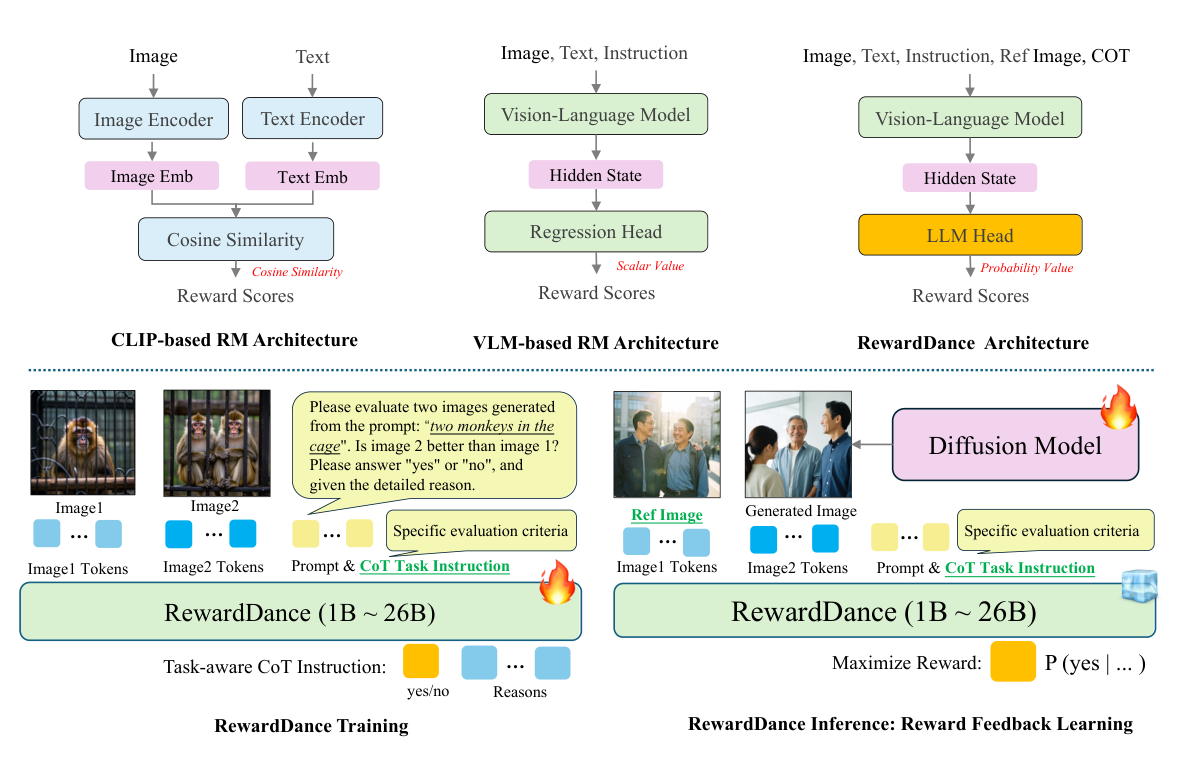
\includegraphics[keepaspectratio,alt={不同奖励建模方式与生成式比较判断 （论文示意，来源：rewarddance）}]{assets/seedance/figures/generative-reward.png}}
\caption{不同奖励建模方式与生成式比较判断 （论文示意，来源：rewarddance）}
\end{figure}

这种形式可以利用视觉语言模型的指令与上下文能力，但模型更大不意味着永远不会被利用。奖励高可能只是模型更擅长命中评分器偏好，而不代表动作、身份和可交付性都提高。

奖励方差也不能直接代替输出多样性。分数变化大，可能来自任务难度差异；分数很集中，也可能是评分器不敏感。应同时看独立人工胜率、重复构图、模板率、动作幅度和任务遵循。

\section{什么时候进入 RL，什么时候停止}\label{seedance-m09-ux4ec0ux4e48ux65f6ux5019ux8fdbux5165-rlux4ec0ux4e48ux65f6ux5019ux505cux6b62}

先做高质量 SFT，再用固定候选重排测试奖励是否与人工一致。只有它能区分真实改善和表面讨好，才适合进一步驱动生成器更新。每轮固定 reward 版本，保留没有参与奖励训练和阈值调整的验证集。

如果奖励持续上涨，人工可用率却下降，或者动作越来越慢、肤质越来越平、构图越来越重复，就应停止并回到数据和奖励定义。优化器负责把模型推向高奖励区域，奖励目标是否代表业务需要，仍必须通过独立评价来确认。

\section{从极简代码到真实实现}\label{seedance-m09-ux4eceux6781ux7b80ux4ee3ux7801ux5230ux771fux5b9eux5b9eux73b0}

组内优势只在同一个提示的候选之间计算，不能把不同任务混成一组：

\begin{verbatim}
# rewards: [batch, group_size]
centered = rewards - rewards.mean(-1, keepdim=True)
advantage = centered / (rewards.std(-1, keepdim=True, correction=0) + 1e-6)
\end{verbatim}

DPO、组内优势和截断目标的核心计算见 \hyperref[code-preference-objectives]{preference\_objectives.py}。完整采样、奖励和更新路径看 \href{https://github.com/XueZeyue/DanceGRPO/blob/15cc71d53cc2e6e18a68ee607d5fb6ba9a99e344/fastvideo/train_grpo_hunyuan.py}{DanceGRPO Hunyuan 训练}。仅有优势公式还不是视觉 GRPO；真实实现还需要 SDE 转移密度、old policy 与时间采样。

\part{替代实现、应用与方案讨论}
% Imported from topics/video-generation/seedance-2.5/architecture.md
\chapter{Wan 基座的增量候选架构}\label{seedance-m12}
\moduleinfo{M12}{增量路线与工程阅读；未运行教学代码}{\hyperref[src-wan-2.1]{\texttt{wan-2.1}}、\hyperref[src-seedance-1.0]{\texttt{seedance-1.0}}、\hyperref[src-phantom]{\texttt{phantom}}、\hyperref[src-long-context-tuning]{\texttt{long-context-tuning}}、\hyperref[src-seedance-2.5-release]{\texttt{seedance-2.5-release}}、\hyperref[src-wan21-code]{\texttt{wan21-code}}、\hyperref[src-diffsynth-code]{\texttt{diffsynth-code}}、\hyperref[src-phantom-code]{\texttt{phantom-code}}、\hyperref[src-longlive-code]{\texttt{longlive-code}}、\hyperref[src-ltx-code]{\texttt{ltx-code}}}

前文主线使用联合音视频基座；这一章另列 Wan 视频单项路线，便于较小规模的机制与适配试验。

前面分别讨论了参考、编辑和长视频，现在尝试把它们接到一个可获得的基座上。先取 Wan-2.1 T2V-1.3B，保留已训练的接口，再逐步增加条件。这样能明确每一步修改了哪里。下面是一套待实验的增量设计，不据此认定它就是 Seedance 2.5 的内部结构。

这条路线适合先研究视频单项能力，音轨可通过后期流程制作。需要在一个主干内联合处理声音、多参考、编辑和长叙事时，另有以 LTX-2 原系列为基础的 \hyperref[seedance-m19]{完整候选架构} 与 \hyperref[seedance-m20]{联合训练配方}；两条路线分别维护潜空间、权重和训练配置。

\section{先保留基座的有效接口}\label{seedance-m12-ux5148ux4fddux7559ux57faux5ea7ux7684ux6709ux6548ux63a5ux53e3}

Wan 的 VAE 使用时间四倍、空间八倍压缩，潜变量为 16 通道；DiT 再采用 \codepath{1×2×2} patch，文本由 umT5 编码并通过交叉注意力进入视觉主干。

\begin{figure}
\centering
\pandocbounded{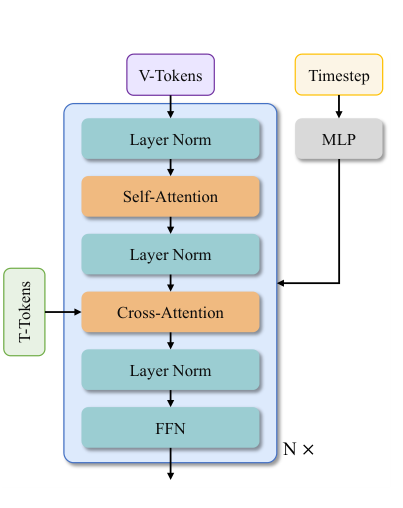
\includegraphics[keepaspectratio,alt={基座的视觉自注意力、文本交叉注意力与前馈模块 （论文示意，来源：wan-2.1）}]{assets/seedance/figures/wan-block.png}}
\caption{基座的视觉自注意力、文本交叉注意力与前馈模块 （论文示意，来源：wan-2.1）}
\end{figure}

先保留这些接口，是因为原权重已经在相应潜变量和文本特征上训练过。另一种 VAE 即使输出相似网格，通道意义、分布和归一化也可能不同；换文本编码器、patch 或位置布局也一样。张量能拼上，还不能说明权重仍在处理它认识的数据。

1.3B 相对适合缩小实验，但推理能运行不等于全参训练资源足够。开始前仍需固定源码、checkpoint、许可证、依赖和硬件基线，再测量实际显存与吞吐。

\section{请求先编译成任务}\label{seedance-m12-ux8bf7ux6c42ux5148ux7f16ux8bd1ux6210ux4efbux52a1}

任务先从用户语言翻译成可计算的条件：主体、镜头、时间、参考用途、必须保持与允许变化的内容。原始要求另外保存，再生成稠密提示，才能检查人数、动作顺序和否定条件有没有在改写中改变。

\begin{verbatim}
用户要求与素材
  → 任务解析与约束检查
  → 素材绑定、参考编码、文本编码
  → 带条件的视频采样
  → VAE 解码、局部合成、音轨处理
  → 自动检查与人工审片
  → 交付或定向返工
\end{verbatim}

如果角色指代或时间尚不明确，后面就没有唯一的绑定对象。缺素材、绑定互相冲突，也应在生成前显式解决，不能把不确定性藏进模型输入，再将模型忽略条件当成一次普通失败。

\section{参考支路怎样增加}\label{seedance-m12-ux53c2ux8003ux652fux8defux600eux6837ux589eux52a0}

先只加入图片身份与外观参考。图片经过基座 VAE、投影和定额池化，形成 \codepath{B,R,d_ref} 的参考记忆；每个 token 携带 role、subject、shot 和时间信息。

在部分主干层后加入门控交叉注意力：

\[
h'_v=h_v+g\operatorname{Attn}(Q_v,K_r,V_r).
\]

插入密度先取每四个 Transformer block 一次，门控零初始化，主干冻结，只训练新支路。这样先看这条路径本身能否学习。随后再比较更密或更疏的插入、不同 token 预算，以及有限 LoRA 解冻；这组初值不是已经证明的最优解。

参考按镜头检索与分配预算，初期可试总计 1024 个 token，同时保留更高预算对照。超额时记录截断项；精细 logo、多人身份和动作视频可能需要不同的编码与预算。

\section{局部编辑为什么另加条件路径}\label{seedance-m12-ux5c40ux90e8ux7f16ux8f91ux4e3aux4ec0ux4e48ux53e6ux52a0ux6761ux4ef6ux8defux5f84}

T2V checkpoint 本身没有自动长出源视频和区域 mask 的接口。编辑因而需要新增源条件支路，读取源 latent、编辑与上下文 mask，再以残差影响主干。目标原来的带噪输入通道先保留，避免新增条件时把旧输入头的权重关系一起改掉。

生成后的局部区域与源帧合成，可使不允许变化的位置直接复用原像素。若目标是姿态或视角变化，则另定义语义与几何保持条件，不能继续使用逐像素不变作为唯一标准。

参考与源条件先分开训练，再分别观察结果。否则身份没保持，可能是参考没有读到，也可能是编辑任务改变了它；两条路径同时变化，就不容易定位原因。

\section{多镜头先编排，再研究原生长上下文}\label{seedance-m12-ux591aux955cux5934ux5148ux7f16ux6392ux518dux7814ux7a76ux539fux751fux957fux4e0aux4e0bux6587}

多镜头也可以从更小的问题开始：先用角色资产和状态记录连接几个短镜头，再显式剪辑。外观、道具归属、位置以及已经发生的事件，都是下一镜头的条件，而不只是给编辑器看的附注。

等短镜头控制可靠，再尝试场景级联合训练和因果续写。前者涉及逐镜头噪声时间，后者还涉及固定历史与缓存失效。它们改变了模型读到什么，不能通过给原输入增加一个长序列参数就得到。

多镜头编排形成三十秒成片，与原生一次生成三十秒，属于不同成果，应使用不同的质量、成本和局部修改标准。

\section{音频与服务层怎样安排}\label{seedance-m12-ux97f3ux9891ux4e0eux670dux52a1ux5c42ux600eux6837ux5b89ux6392}

起步版本可以独立配音、制作音效并确定性混流。强口型或动作音效同步任务，再单独引入音频 codec、音频主干与联合训练；需要对齐数据、语言覆盖和同步验证。

媒体与 latent 放对象存储，任务数据库保存版本和依赖。CPU 解码、GPU 描述与编码、训练、推理分别成为 worker；小规模用本地 manifest 和简单队列即可，吞吐成为瓶颈后再增加分布式调度。

每次输出应能反查模型、适配器、数据、提示、参考、种子和 scheduler。用户再次生成只是行为信号，需结合失败标注才能进入训练反馈。

\section{用阶段门槛控制复杂度}\label{seedance-m12-ux7528ux9636ux6bb5ux95e8ux69dbux63a7ux5236ux590dux6742ux5ea6}

{\def\LTcaptype{table} % do not increment counter
\small\setlength{\tabcolsep}{3pt}\renewcommand{\arraystretch}{1.18}
\begin{longtable}[]{@{}
  >{\raggedright\arraybackslash}p{(\linewidth - 2\tabcolsep) * \real{0.2200}}
  >{\raggedright\arraybackslash}p{(\linewidth - 2\tabcolsep) * \real{0.7800}}@{}}
\toprule\noalign{}
\begin{minipage}[b]{\linewidth}\raggedright
阶段
\end{minipage} & \begin{minipage}[b]{\linewidth}\raggedright
需要证明的结果
\end{minipage} \\
\midrule\noalign{}
\endhead
\bottomrule\noalign{}
\endlastfoot
原版基线 & 短片生成、VAE 重建、计时与重复运行正确 \\
图片参考 & 一到四图较纯文本改善身份，动作不过度退化 \\
区域编辑 & 目标变化、非目标保持、时间边界稳定 \\
多镜头 & 角色与道具状态在两到四镜头间持续成立 \\
原生长上下文 & 长 rollout 稳定，缓存与重算等价 \\
联合音频 & 同步、音质和视频质量共同达到任务标准 \\
\end{longtable}
}

这样分阶段，目的是让每项能力有可观察的任务和退出条件。某条路线暂时没有收益，还能保留已经验证的部件；如果只以架构图是否完整为目标，未解决的依赖就会一路进入后续系统。

\section{真实工程从哪里进入}\label{seedance-m12-ux771fux5b9eux5de5ux7a0bux4eceux54eaux91ccux8fdbux5165}

基础生成选 \href{https://github.com/Wan-Video/Wan2.1}{Wan}，训练入口选 \href{https://github.com/modelscope/DiffSynth-Studio}{DiffSynth}，参考推理看 \href{https://github.com/Phantom-video/Phantom}{Phantom-Wan}，长视频单独看 \href{https://github.com/NVlabs/LongLive/blob/31c70d9071cd7851d82939806dc9fac645fcabe5/LongLive1.0/inference.py}{LongLive1.0}，联合音视频另走 \href{https://github.com/Lightricks/LTX-2}{LTX}。每条路线的固定版本、接口差异和代码入口列在 \hyperref[seedance-m15]{代码路线与仓库选择}；本地只保留讲机制的极简片段，不另搭一个训练框架。

% Imported from topics/video-generation/seedance-2.5/training.md
\chapter{M13 增量训练阶段与停止条件}\label{seedance-m13}
\moduleinfo{M13}{增量路线与工程阅读；未运行教学代码}{\hyperref[src-seedance-1.0]{\texttt{seedance-1.0}}、\hyperref[src-seedance-1.5-pro]{\texttt{seedance-1.5-pro}}、\hyperref[src-wan-2.1]{\texttt{wan-2.1}}、\hyperref[src-long-context-tuning]{\texttt{long-context-tuning}}、\hyperref[src-dancegrpo]{\texttt{dancegrpo}}、\hyperref[src-rewarddance]{\texttt{rewarddance}}、\hyperref[src-diffsynth-code]{\texttt{diffsynth-code}}、\hyperref[src-longlive-code]{\texttt{longlive-code}}、\hyperref[src-ltx-code]{\texttt{ltx-code}}、\hyperref[src-dancegrpo-code]{\texttt{dancegrpo-code}}}


训练一个完整视频基础模型，与在现有模型上增加业务能力，需要完全不同的数据和预算。对于可控参考、局部编辑和多镜头任务，更容易执行的路线是保留已训练好的基座，先证明数据与损失链路正确，再逐项增加能力。

下面给出以 Wan-2.1 T2V-1.3B 为候选基座的训练流程。参数是初始试验配方，尚未经过实际训练验证；是否扩大训练，取决于每阶段的测量结果。

本流程面向较轻的视频增量试验。需要训练统一参考、编辑、结构条件和原生音视频时，采用单独的 \hyperref[seedance-m20]{联合候选训练配方}，与相应 \hyperref[seedance-m19]{完整架构} 配套；Wan 阶段的 latent、参数组和优化器状态不能直接挪用。

\section{训练阶段为什么要分开}\label{seedance-m13-ux8badux7ec3ux9636ux6bb5ux4e3aux4ec0ux4e48ux8981ux5206ux5f00}

典型生成系统先通过预训练学习宽分布，再用继续训练、高质量 SFT 和反馈优化强化能力；高分辨率精修模型也可能有自己的训练路径。

\begin{figure}
\centering
\pandocbounded{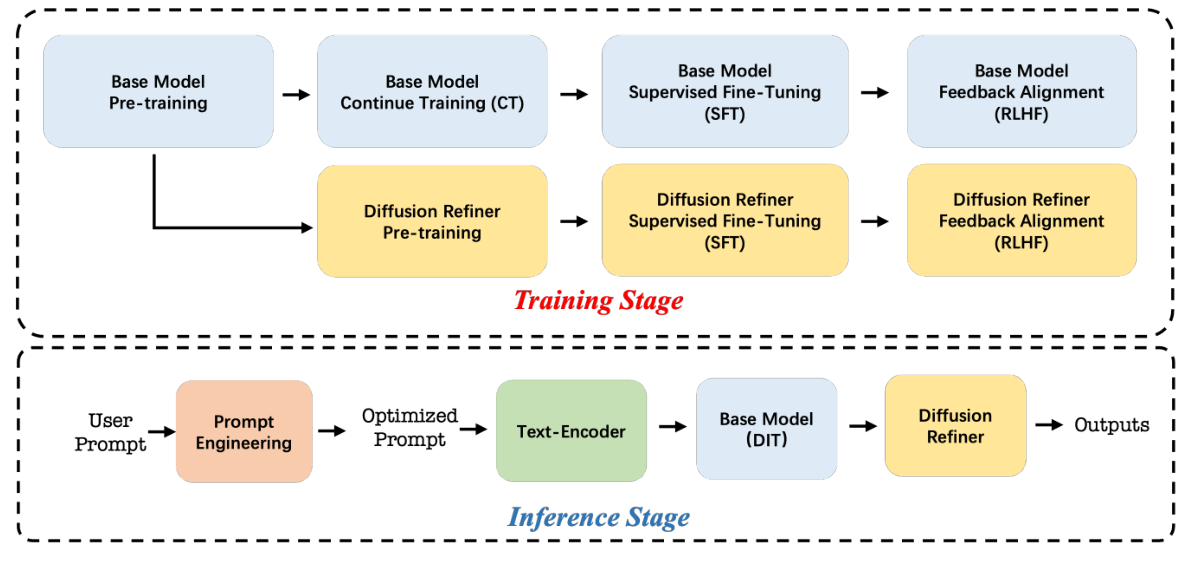
\includegraphics[keepaspectratio,alt={基础模型与精修模型的训练及推理组织 （论文示意，来源：seedance-1.0）}]{assets/seedance/figures/training-pipeline.png}}
\caption{基础模型与精修模型的训练及推理组织 （论文示意，来源：seedance-1.0）}
\end{figure}

分阶段的作用是改变数据分布、训练目标或可训练参数，同时保留上一步的能力。它不意味着必须照搬某个大模型的全部预训练规模。预算有限时，应先完成基座适配，而不是从头复刻基础训练。

\section{第一步：证明原版模型和数据链路正确}\label{seedance-m13-ux7b2cux4e00ux6b65ux8bc1ux660eux539fux7248ux6a21ux578bux548cux6570ux636eux94feux8defux6b63ux786e}

固定源码、模型、VAE、文本编码器、scheduler 和环境版本。先运行原版生成与真实视频重建，保存固定种子的输出，记录数值精度、非确定性算子、显存和时间。

选择 32 个有权使用的真实样本作调试集，另留来源隔离的验证集。起初关闭随机增强与条件 dropout，检查模型能否过拟合这些样本，并测试换文本、移除参考后输出是否相应变化。调试集的重现不能作为泛化成绩，但能快速发现目标符号、latent 缩放和条件接线错误。

必须测到有效样本/秒、有效 token/秒、step 时间、峰值显存和梯度范数，才有依据确定后续 batch、分辨率和预算。

\section{第二步：只训练图片参考支路}\label{seedance-m13-ux7b2cux4e8cux6b65ux53eaux8badux7ec3ux56feux7247ux53c2ux8003ux652fux8def}

冻结原 VAE、文本编码器和主干，训练参考特征投影、池化、角色嵌入和门控交叉注意力。先保留纯文本任务作回归，再比较少量主干 LoRA 是否带来额外收益。

{\def\LTcaptype{table} % do not increment counter
\small\setlength{\tabcolsep}{3pt}\renewcommand{\arraystretch}{1.18}
\begin{longtable}[]{@{}
  >{\raggedright\arraybackslash}p{(\linewidth - 2\tabcolsep) * \real{0.2200}}
  >{\raggedright\arraybackslash}p{(\linewidth - 2\tabcolsep) * \real{0.7800}}@{}}
\toprule\noalign{}
\begin{minipage}[b]{\linewidth}\raggedright
项目
\end{minipage} & \begin{minipage}[b]{\linewidth}\raggedright
初始候选
\end{minipage} \\
\midrule\noalign{}
\endhead
\bottomrule\noalign{}
\endlastfoot
输入桶 & 例如 \(256\times448\)、33 帧；需符合实际基座和预处理约定 \\
精度 & 硬件支持时 BF16 \\
优化器 & AdamW，学习率 \(10^{-4}\)，\(\beta=(0.9,0.999)\)，\(\epsilon=10^{-8}\) \\
权重衰减 & 0.01 \\
有效全局 batch & 8 个样本 \\
梯度裁剪 & 全局范数 1.0，同时记录裁剪前范数 \\
预热与步数 & 预热 100 步，总计 1000 步的 pilot \\
条件 dropout & 文本与参考各 0.1，独立采样 \\
验证与保存 & 每 100 步固定验证，保存可恢复状态与独立最佳点 \\
\end{longtable}
}

全局 batch 由单卡 microbatch、梯度累积和卡数共同决定：

\[
B_{\mathrm{global}}=B_{\mathrm{micro}}\times K_{\mathrm{accum}}\times N_{\mathrm{GPU}}.
\]

目标 batch 为 8、每卡 microbatch 为 1 时，累积步数需与卡数匹配，不能简单使用向下取整悄悄改变有效 batch。损失应按有效元素归一化，避免长片或大图仅因 token 更多而主导更新。

低分辨率可以降低验证成本，但形状合法不等于分布适配。身份改善、动作退化和纯文本回归都要通过固定任务集观察。随机裁剪、位置变换和更大分辨率应在基线正确后逐项加入，并同步变换 mask 与框。

\section{第三步：训练区域和区间编辑}\label{seedance-m13-ux7b2cux4e09ux6b65ux8badux7ec3ux533aux57dfux548cux533aux95f4ux7f16ux8f91}

新增源条件支路，输入源 latent、编辑与上下文 mask、修改指令和可选参考。先冻结已验证的参考支路，在受控重渲染真值上验证，再混入人工真实编辑对和弱监督数据。

起步任务可以是服装颜色、局部物体和背景替换；相机视角、全局光照和复杂遮挡另立切片。损失掩码、非目标保持损失以及最终像素合成要明确分工。latent 一致不保证像素无变化，外区直接复用也不保证边缘光照自然。

只有目标变化、外区保持和时间边界同时改善，才扩大训练；否则应先回到数据配对、mask 和任务约束，而不是立即用更复杂奖励压高总分。

\section{第四步：扩大到场景级多镜头}\label{seedance-m13-ux7b2cux56dbux6b65ux6269ux5927ux5230ux573aux666fux7ea7ux591aux955cux5934}

先做两镜头，再做四镜头，样本包含全局角色与环境、逐镜头动作、道具状态和时间顺序。按 token 预算组 batch，跨场景 packing 使用隔离 mask，避免不同故事互相读取。

异步噪声需要逐镜头噪声时间与相应调制。如果基座仅支持全局 timestep，必须增加并训练正确的逐 token 条件，而不是只替换 attention mask。

双向场景模型先作为联合生成对照，因果续写另做适配并独立保存版本。缓存先通过完整重算等价检查，再测速度。训练时逐步加入自生成历史，观察它与真实历史之间的分布差异；长程评测按时间段看漂移，不能只报告整段平均。

\section{第五步：把联合音频作为独立工程}\label{seedance-m13-ux7b2cux4e94ux6b65ux628aux8054ux5408ux97f3ux9891ux4f5cux4e3aux72ecux7acbux5de5ux7a0b}

需要先确定音频 codec 和主干，明确采样率、token rate、延迟与授权数据。先冻结视频，训练音频及跨模态门控，再根据同步和音质收益决定是否联合解冻。

缺失音轨的样本不计算音频目标，真实静音保留监督。嘴形、动作音效、语言、音色和音乐控制分别评估；不能只因为音轨时长对上，就认为联合生成已经正确。

\section{偏好优化和蒸馏放在哪一步}\label{seedance-m13-ux504fux597dux4f18ux5316ux548cux84b8ux998fux653eux5728ux54eaux4e00ux6b65}

先做高质量 SFT，再验证固定候选的奖励重排是否与人工一致。奖励可靠后才考虑 RL；低步数蒸馏再以已确定的 teacher 和任务分布展开。生成器、奖励模型、数据和 student 都需独立版本，防止边训练边换评价标准。

若奖励上涨但人工通过率下降，或者动作和构图趋于单一，应停止回滚。少步数 student 也需要与 teacher 比较身份、动作与交付可用率，不能只比较每秒出多少帧。

\section{怎样保证训练能恢复、成本能估算}\label{seedance-m13-ux600eux6837ux4fddux8bc1ux8badux7ec3ux80fdux6062ux590dux6210ux672cux80fdux4f30ux7b97}

保存模型权重之外，还要保存 optimizer、scheduler、全局步数、所有随机状态、数据采样位置和梯度累积状态。一次中断后，应对照不中断运行的下一批样本 ID 与损失，验证恢复语义。只加载权重继续跑不等于精确续训。

预算依据实测 step 时间计算：

\[
T_{\mathrm{hours}}=\frac{N_{\mathrm{steps}}t_{\mathrm{step}}}{3600},
\qquad
C_{\mathrm{GPU\,hours}}=T_{\mathrm{hours}}N_{\mathrm{GPU}}.
\]

还要另计数据制作、验证、checkpoint 和失败重跑。学习率、有效 batch、分辨率和训练参数范围改变后，吞吐可能重新变化；预算应随测量更新，而不是由模型参数量单独推断。

\section{真实工程从哪里进入}\label{seedance-m13-ux771fux5b9eux5de5ux7a0bux4eceux54eaux91ccux8fdbux5165}

LoRA 与全参训练先从 \href{https://github.com/modelscope/DiffSynth-Studio/blob/d32f72424cd22bc0ea8100cc57559149b4eac933/examples/wanvideo/model_training/train.py}{DiffSynth Wan train.py} 和 \href{https://github.com/modelscope/DiffSynth-Studio/blob/d32f72424cd22bc0ea8100cc57559149b4eac933/examples/wanvideo/model_training/lora/Wan2.1-T2V-1.3B.sh}{LoRA 配方} 阅读；流式长训练看 \href{https://github.com/NVlabs/LongLive/blob/31c70d9071cd7851d82939806dc9fac645fcabe5/LongLive1.0/pipeline/streaming_training.py}{LongLive1.0 streaming\_training}；联合音视频看 \href{https://github.com/Lightricks/LTX-2/blob/daa6b16fc7f0f1628f2c9e36a303e3312b333cc6/packages/ltx-trainer/README.md}{LTX trainer}；策略优化看 \href{https://github.com/XueZeyue/DanceGRPO/blob/15cc71d53cc2e6e18a68ee607d5fb6ba9a99e344/fastvideo/train_grpo_hunyuan.py}{DanceGRPO 视频训练}。这些是各自框架中的真实入口，环境、数据和权重按对应版本匹配，未在此执行训练。

% Imported from docs/code-paths.md
\chapter{M15 机制代码与真实工程路线}\label{seedance-m15}
\moduleinfo{M15}{增量路线与工程阅读；未运行教学代码}{\hyperref[src-wan21-code]{\texttt{wan21-code}}、\hyperref[src-diffsynth-code]{\texttt{diffsynth-code}}、\hyperref[src-phantom-code]{\texttt{phantom-code}}、\hyperref[src-longlive-code]{\texttt{longlive-code}}、\hyperref[src-vincie-code]{\texttt{vincie-code}}、\hyperref[src-ltx-code]{\texttt{ltx-code}}、\hyperref[src-dancegrpo-code]{\texttt{dancegrpo-code}}、\hyperref[src-tarsier-code]{\texttt{tarsier-code}}、\hyperref[src-ltx-original-code]{\texttt{ltx-original-code}}、\hyperref[src-vace-code]{\texttt{vace-code}}、\hyperref[src-videocof-code]{\texttt{videocof-code}}}


理解一个视频模块时，几十行代码往往比完整训练框架更清楚；真正制作数据、训练和生成时，则应使用已经组织好模型加载、调度、分布式和输出流程的工程。这两种代码各有用途，不需要把教学片段扩写成另一个大型框架。

这里把十六份本地机制示例与十个上游仓库对应起来，其中 LTX 原系列与当前版本分别固定。仓库版本、源码入口和许可证已经查阅，未运行模型或训练，也不据此承诺它们满足某个具体业务的效果与硬件条件。

\section{用极简代码理解一件事}\label{seedance-m15-ux7528ux6781ux7b80ux4ee3ux7801ux7406ux89e3ux4e00ux4ef6ux4e8b}

{\def\LTcaptype{table} % do not increment counter
\small\setlength{\tabcolsep}{3pt}\renewcommand{\arraystretch}{1.18}
\begin{longtable}[]{@{}
  >{\raggedright\arraybackslash}p{(\linewidth - 6\tabcolsep) * \real{0.1600}}
  >{\raggedright\arraybackslash}p{(\linewidth - 6\tabcolsep) * \real{0.2800}}
  >{\raggedright\arraybackslash}p{(\linewidth - 6\tabcolsep) * \real{0.2800}}
  >{\raggedright\arraybackslash}p{(\linewidth - 6\tabcolsep) * \real{0.2800}}@{}}
\toprule\noalign{}
\begin{minipage}[b]{\linewidth}\raggedright
机制
\end{minipage} & \begin{minipage}[b]{\linewidth}\raggedright
本地示例
\end{minipage} & \begin{minipage}[b]{\linewidth}\raggedright
阅读重点
\end{minipage} & \begin{minipage}[b]{\linewidth}\raggedright
真实实现入口
\end{minipage} \\
\midrule\noalign{}
\endhead
\bottomrule\noalign{}
\endlastfoot
因果时空卷积 & \hyperref[code-causal-conv]{causal\_conv.py} & 时间左 padding 与 stride/dilation & Wan VAE \\
流匹配 & \hyperref[code-flow-matching]{flow\_matching.py} & noisy、速度目标、有效区损失、Euler & Wan 采样与 DiffSynth 训练 \\
三维 RoPE & \hyperref[code-rope]{rope.py} & 按通道分轴旋转 Q/K & Wan / VINCIE / LTX RoPE \\
空间与时间注意力 & \hyperref[code-attention-layout]{attention\_layout.py} & 哪些维合成 batch，哪些合成序列 & Wan block / VINCIE MM attention \\
参考条件 & \hyperref[code-reference-adapter]{reference\_adapter.py} & query、reference K/V、绑定 mask、门控 & Phantom-Wan \\
区间与区域编辑 & \hyperref[code-local-edit]{local\_edit.py} & 时间选择、已知区重噪、最终像素保留 & VINCIE 图像编辑 / LTX 条件流水线 \\
联合音视频 & \hyperref[code-audio-video-exchange]{audio\_video\_exchange.py} & 双向读取更新前状态 & LTX AV Transformer \\
偏好优化 & \hyperref[code-preference-objectives]{preference\_objectives.py} & DPO、组内优势、clipped objective & DanceGRPO \\
缓存失效 & \hyperref[code-cache-context]{cache\_context.py} & 历史与条件不变才能复用 & LongLive 因果推理 \\
参考时间门 & \hyperref[code-reference-timing]{reference\_timing.py} & 物理时间、软区间偏置；归属mask与null token另接 & 候选支路；不是WeRoPE复现 \\
统一视觉条件 & \hyperref[code-condition-unit]{condition\_unit.py} & 待变/保留拆分、时间与空间编辑范围 & VACE条件与mask预处理 \\
相机射线 & \hyperref[code-camera-rays]{camera\_rays.py} & camera-to-world、方向与矩、单位一致 & 结构条件投影由候选工程新增 \\
候选参考残差 & \hyperref[code-gated-condition]{gated\_condition.py} & 输入/输出宽度、零门控、非零投影初始化 & LTX块循环需新增支路调用 \\
干净条件与活动目标 & \hyperref[code-condition-state]{condition\_state.py} & 逐token sigma、逐样本Euler步长、已知区覆盖 & LTX训练strategy与采样器需新增任务状态 \\
音视频块因果 & \hyperref[code-block-causal-mask]{block\_causal\_mask.py} & 视频/音频self和双向AV都限制未来 & LongLive机制；LTX四类调用需改造 \\
逐样本有效损失 & \hyperref[code-masked-sample-loss]{masked\_sample\_loss.py} & 先对有效元素平均，排除没有监督的样本 & 自定义strategy；分布式计数另接 \\
\end{longtable}
}

示例的约束写在各文件开头：有的省略多头，有的要求每个 query 至少有一个有效参考，有的只支持整除的空间窗口。它们解释依赖关系，不负责补齐生产环境中的所有分支，也不能直接加载这些仓库的 checkpoint。

\section{从 Wan 建立基础生成链路}\label{seedance-m15-ux4ece-wan-ux5efaux7acbux57faux7840ux751fux6210ux94feux8def}

\href{https://github.com/Wan-Video/Wan2.1}{Wan-Video/Wan2.1} 适合阅读和使用基础文生视频、图生视频、VAE 与 DiT。固定版本为 \codepath{9737cba9c1c3c4d04b33fcad41c111989865d315}。

\begin{itemize}
\tightlist
\item
  \href{https://github.com/Wan-Video/Wan2.1/blob/9737cba9c1c3c4d04b33fcad41c111989865d315/generate.py}{生成入口 generate.py}：参数、任务选择和结果输出。
\item
  \href{https://github.com/Wan-Video/Wan2.1/blob/9737cba9c1c3c4d04b33fcad41c111989865d315/wan/text2video.py}{text2video.py}：文本、噪声、scheduler 和解码怎样衔接。
\item
  \href{https://github.com/Wan-Video/Wan2.1/blob/9737cba9c1c3c4d04b33fcad41c111989865d315/wan/modules/vae.py}{vae.py}：\codepath{CausalConv3d}、上下采样、encoder/decoder 和缓存。
\item
  \href{https://github.com/Wan-Video/Wan2.1/blob/9737cba9c1c3c4d04b33fcad41c111989865d315/wan/modules/model.py}{model.py}：\codepath{WanAttentionBlock}、\codepath{rope_apply} 与主干。
\end{itemize}

阅读顺序可先从 \codepath{generate.py} 跟进 \codepath{text2video.py}，再进入模块。只看 VAE 中的一个卷积类，无法推导完整视频采样流程。

\section{用 DiffSynth-Studio 接入真实训练}\label{seedance-m15-ux7528-diffsynth-studio-ux63a5ux5165ux771fux5b9eux8badux7ec3}

\href{https://github.com/modelscope/DiffSynth-Studio}{modelscope/DiffSynth-Studio} 提供 Wan 的推理、LoRA 和全参训练。固定版本为 \codepath{d32f72424cd22bc0ea8100cc57559149b4eac933}。

\begin{itemize}
\tightlist
\item
  \href{https://github.com/modelscope/DiffSynth-Studio/blob/d32f72424cd22bc0ea8100cc57559149b4eac933/examples/wanvideo/model_training/train.py}{训练入口 train.py}：\codepath{WanTrainingModule}、数据参数和训练组件。
\item
  \href{https://github.com/modelscope/DiffSynth-Studio/blob/d32f72424cd22bc0ea8100cc57559149b4eac933/examples/wanvideo/model_training/lora/Wan2.1-T2V-1.3B.sh}{1.3B LoRA 配方}：数据路径、模型组件、学习率、rank 与 target modules。
\item
  \href{https://github.com/modelscope/DiffSynth-Studio/blob/d32f72424cd22bc0ea8100cc57559149b4eac933/examples/wanvideo/model_training/full/Wan2.1-T2V-1.3B.sh}{1.3B 全参配方}：与 LoRA 比较哪些参数进入训练。
\item
  \href{https://github.com/modelscope/DiffSynth-Studio/blob/d32f72424cd22bc0ea8100cc57559149b4eac933/examples/wanvideo/model_inference/Wan2.1-T2V-1.3B.py}{1.3B 推理样例}：模型加载与 pipeline 调用。
\end{itemize}

真实实施可先沿用这个训练框架，再增加业务数据和所需条件路径。现成 LoRA 能调整模型行为，但不会自动获得角色绑定、任意参考数量或时间戳编辑；这些能力还依赖对应模型接口与数据任务。

\section{用 Phantom-Wan 研究主体参考}\label{seedance-m15-ux7528-phantom-wan-ux7814ux7a76ux4e3bux4f53ux53c2ux8003}

\href{https://github.com/Phantom-video/Phantom}{Phantom-video/Phantom} 的公开实现建立在 Wan 上，固定版本为 \codepath{bd84b602dcc949e23c89cbbf266b6f5975f2f025}。

\begin{itemize}
\tightlist
\item
  \href{https://github.com/Phantom-video/Phantom/blob/bd84b602dcc949e23c89cbbf266b6f5975f2f025/generate.py}{generate.py}：参考图片列表与主体生成参数。
\item
  \href{https://github.com/Phantom-video/Phantom/blob/bd84b602dcc949e23c89cbbf266b6f5975f2f025/phantom_wan/subject2video.py}{subject2video.py}：参考编码与采样编排。
\item
  \href{https://github.com/Phantom-video/Phantom/blob/bd84b602dcc949e23c89cbbf266b6f5975f2f025/phantom_wan/modules/model.py}{model.py}：参考条件怎样进入主干。
\end{itemize}

该版本提供参考推理，README 的训练代码项目仍未勾选。因此它适合作为参考生成和结构阅读入口，不能直接称为可用的完整训练仓库。公开的 Phantom-Wan 与论文内部基座也需要区分。

\section{从 LongLive1.0 阅读长视频训练与缓存}\label{seedance-m15-ux4ece-longlive1.0-ux9605ux8bfbux957fux89c6ux9891ux8badux7ec3ux4e0eux7f13ux5b58}

\href{https://github.com/NVlabs/LongLive}{NVlabs/LongLive} 固定版本为 \codepath{31c70d9071cd7851d82939806dc9fac645fcabe5}。仓库已同时包含多个后续项目，研究原始长视频框架应进入 \codepath{LongLive1.0/}。

\begin{itemize}
\tightlist
\item
  \href{https://github.com/NVlabs/LongLive/blob/31c70d9071cd7851d82939806dc9fac645fcabe5/LongLive1.0/inference.py}{inference.py} 与 \href{https://github.com/NVlabs/LongLive/blob/31c70d9071cd7851d82939806dc9fac645fcabe5/LongLive1.0/train.py}{train.py}：整体入口。
\item
  \href{https://github.com/NVlabs/LongLive/blob/31c70d9071cd7851d82939806dc9fac645fcabe5/LongLive1.0/pipeline/causal_inference.py}{causal\_inference.py}：当前块去噪、历史缓存及窗口组织。
\item
  \href{https://github.com/NVlabs/LongLive/blob/31c70d9071cd7851d82939806dc9fac645fcabe5/LongLive1.0/pipeline/streaming_training.py}{streaming\_training.py}：流式训练如何使用历史。
\item
  \href{https://github.com/NVlabs/LongLive/blob/31c70d9071cd7851d82939806dc9fac645fcabe5/LongLive1.0/wan/modules/causal_model.py}{causal\_model.py}：\codepath{CausalWanSelfAttention} 和缓存数据路径。
\end{itemize}

这里的价值是读取``模型、训练分布、缓存''怎样配套，而不是把缓存类单独移植到任意双向扩散模型。它也不是 Seedance 已确认的内部实现。

\section{从 VINCIE 阅读多轮编辑与交错序列}\label{seedance-m15-ux4ece-vincie-ux9605ux8bfbux591aux8f6eux7f16ux8f91ux4e0eux4ea4ux9519ux5e8fux5217}

\href{https://github.com/ByteDance-Seed/VINCIE}{ByteDance-Seed/VINCIE} 固定版本为 \codepath{97cd2c5701e694dabcfea320c0cf59893d427fab}。

\begin{itemize}
\tightlist
\item
  \href{https://github.com/ByteDance-Seed/VINCIE/blob/97cd2c5701e694dabcfea320c0cf59893d427fab/generate.py}{generate.py}：\codepath{VINCIEGenerator} 多轮图像编辑入口。
\item
  \href{https://github.com/ByteDance-Seed/VINCIE/blob/97cd2c5701e694dabcfea320c0cf59893d427fab/configs/generate.yaml}{生成配置}：模型与采样配置。
\item
  \href{https://github.com/ByteDance-Seed/VINCIE/blob/97cd2c5701e694dabcfea320c0cf59893d427fab/models/dit/blocks/attention/mmattn.py}{mmattn.py}：联合多模态与窗口注意力。
\item
  \href{https://github.com/ByteDance-Seed/VINCIE/blob/97cd2c5701e694dabcfea320c0cf59893d427fab/models/dit/rope.py}{rope.py}：多模态位置编码。
\end{itemize}

它直接处理的是多轮图像编辑，不能把这个生成入口当成通用视频时间戳编辑。图像上下文方法怎样传播到时间连续的视频，是另一层任务和实现。

\section{用 LTX 阅读可实现的联合音视频}\label{seedance-m15-ux7528-ltx-ux9605ux8bfbux53efux5b9eux73b0ux7684ux8054ux5408ux97f3ux89c6ux9891}

\href{https://github.com/Lightricks/LTX-2}{Lightricks/LTX-2} 固定版本为 \codepath{daa6b16fc7f0f1628f2c9e36a303e3312b333cc6}。

\begin{itemize}
\tightlist
\item
  \href{https://github.com/Lightricks/LTX-2/blob/daa6b16fc7f0f1628f2c9e36a303e3312b333cc6/packages/ltx-core/src/ltx_core/model/transformer/transformer.py}{transformer.py}：\codepath{BasicAVTransformerBlock} 的视频/音频交互。
\item
  \href{https://github.com/Lightricks/LTX-2/blob/daa6b16fc7f0f1628f2c9e36a303e3312b333cc6/packages/ltx-core/src/ltx_core/model/transformer/rope.py}{rope.py}：位置与频率实现。
\item
  \href{https://github.com/Lightricks/LTX-2/blob/daa6b16fc7f0f1628f2c9e36a303e3312b333cc6/packages/ltx-pipelines/README.md}{推理说明}：选择模型对应的 pipeline。
\item
  \href{https://github.com/Lightricks/LTX-2/blob/daa6b16fc7f0f1628f2c9e36a303e3312b333cc6/packages/ltx-trainer/README.md}{训练说明} 与 \href{https://github.com/Lightricks/LTX-2/blob/daa6b16fc7f0f1628f2c9e36a303e3312b333cc6/packages/ltx-trainer/configs/av2av_ic_lora.yaml}{音视频条件配置}：真实训练路线。
\end{itemize}

当前版本覆盖多个 LTX 型号，模型、codec、文本组件与 LoRA 要按对应说明匹配。代码是 Apache-2.0，模型使用单独的 Community License；这两类许可不能混为一项。LTX 可作为联合音视频工程的独立选择，不能直接成为 Wan 的兼容音频插件。

\section{将 LTX 原系列固定为共同主干}\label{seedance-m15-ux5c06-ltx-ux539fux7cfbux5217ux56faux5b9aux4e3aux5171ux540cux4e3bux5e72}

完整候选设计选择初始公开系列，另固定 \codepath{bd92a5f408eb8c99f8c05e9fe2fcaaec8b56b638}，避免后续型号的文本、codec与训练配置混入。阅读顺序是表示、主干、训练策略：

\begin{itemize}
\tightlist
\item
  \href{https://github.com/Lightricks/LTX-2/blob/bd92a5f408eb8c99f8c05e9fe2fcaaec8b56b638/packages/ltx-core/src/ltx_core/types.py}{types.py}：视频/音频latent布局及尺寸约定。
\item
  \href{https://github.com/Lightricks/LTX-2/blob/bd92a5f408eb8c99f8c05e9fe2fcaaec8b56b638/packages/ltx-core/src/ltx_core/model/transformer/transformer.py}{transformer.py}：原生AV交互、调制和门控。
\item
  \href{https://github.com/Lightricks/LTX-2/blob/bd92a5f408eb8c99f8c05e9fe2fcaaec8b56b638/packages/ltx-core/src/ltx_core/model/video_vae/video_vae.py}{video\_vae.py}：视频编码、解码与原生归一化。
\item
  \href{https://github.com/Lightricks/LTX-2/blob/bd92a5f408eb8c99f8c05e9fe2fcaaec8b56b638/packages/ltx-trainer/configs/ltx2_av_lora.yaml}{音视频LoRA配置} 与 \href{https://github.com/Lightricks/LTX-2/blob/bd92a5f408eb8c99f8c05e9fe2fcaaec8b56b638/packages/ltx-trainer/configs/ltx2_v2v_ic_lora.yaml}{视频条件IC-LoRA配置}：已有策略、组件和参数组的落地起点。
\item
  \href{https://github.com/Lightricks/LTX-2/blob/bd92a5f408eb8c99f8c05e9fe2fcaaec8b56b638/packages/ltx-core/src/ltx_core/model/transformer/model.py}{model.py} 与 \href{https://github.com/Lightricks/LTX-2/blob/bd92a5f408eb8c99f8c05e9fe2fcaaec8b56b638/packages/ltx-core/src/ltx_core/model/transformer/transformer_args.py}{transformer\_args.py}：块循环、逐token噪声调制及候选支路插入位置。
\item
  \href{https://github.com/Lightricks/LTX-2/blob/bd92a5f408eb8c99f8c05e9fe2fcaaec8b56b638/packages/ltx-trainer/src/ltx_trainer/training_strategies/text_to_video.py}{text\_to\_video.py} 与 \href{https://github.com/Lightricks/LTX-2/blob/bd92a5f408eb8c99f8c05e9fe2fcaaec8b56b638/packages/ltx-trainer/src/ltx_trainer/training_strategies/video_to_video.py}{video\_to\_video.py}：前者可联合训练AV，后者是视频参考拼接；不能直接把后者当成联合音频编辑。
\item
  \href{https://github.com/Lightricks/LTX-2/blob/bd92a5f408eb8c99f8c05e9fe2fcaaec8b56b638/packages/ltx-trainer/src/ltx_trainer/timestep_samplers.py}{timestep\_samplers.py} 与 \href{https://github.com/Lightricks/LTX-2/blob/bd92a5f408eb8c99f8c05e9fe2fcaaec8b56b638/packages/ltx-trainer/src/ltx_trainer/trainer.py}{trainer.py}：长度外推、参数收集与权重保存；新增模块和完整恢复状态需要显式扩展。
\end{itemize}

这些配置没有自动包含候选方案的多参考池化、角色时间绑定、VACE式支路或因果续写；新增接口与任务仍需实现。该历史commit的 \href{https://github.com/Lightricks/LTX-2/blob/bd92a5f408eb8c99f8c05e9fe2fcaaec8b56b638/LICENSE}{根许可证} 是 LTX-2 Community License，应按历史版本记录，不能回填当前版本的Apache代码许可结论。

\section{从 VACE 阅读统一视觉条件}\label{seedance-m15-ux4ece-vace-ux9605ux8bfbux7edfux4e00ux89c6ux89c9ux6761ux4ef6}

\href{https://github.com/ali-vilab/VACE}{ali-vilab/VACE} 固定 \codepath{48eb44f1c4be87cc65a98bff985a26976841e9f3}，代码Apache-2.0。它把不同视觉条件组织为帧与mask，再接入相应基座。

\begin{itemize}
\tightlist
\item
  \href{https://github.com/ali-vilab/VACE/blob/48eb44f1c4be87cc65a98bff985a26976841e9f3/vace/vace_preproccess.py}{vace\_preproccess.py}：条件预处理入口，文件名沿用上游拼写。
\item
  \href{https://github.com/ali-vilab/VACE/blob/48eb44f1c4be87cc65a98bff985a26976841e9f3/vace/annotators/mask.py}{mask.py}：编辑区域和mask组织。
\item
  \href{https://github.com/ali-vilab/VACE/blob/48eb44f1c4be87cc65a98bff985a26976841e9f3/vace/vace_wan_inference.py}{vace\_wan\_inference.py}：条件、checkpoint与Wan采样链路怎样配合。
\end{itemize}

这是可用视觉控制工程的入口，但不同基座分支有各自权重和条件层。即使目录中出现LTX分支，也不代表能直接加载到这里固定的LTX-2原系列。

\section{从 VideoCoF 阅读区域中间表示}\label{seedance-m15-ux4ece-videocof-ux9605ux8bfbux533aux57dfux4e2dux95f4ux8868ux793a}

\href{https://github.com/knightyxp/VideoCoF}{knightyxp/VideoCoF} 固定 \codepath{f45b8009616b3ef8e2024a7da585249b4c74fc2b}，代码Apache-2.0，包含Wan/VideoX-Fun的推理与训练入口。

\begin{itemize}
\tightlist
\item
  \href{https://github.com/knightyxp/VideoCoF/blob/f45b8009616b3ef8e2024a7da585249b4c74fc2b/examples/wan2.1/predict_v2v_cot_json.py}{predict\_v2v\_cot\_json.py}：源视频、指令与区域式编辑的推理组织。
\item
  \href{https://github.com/knightyxp/VideoCoF/blob/f45b8009616b3ef8e2024a7da585249b4c74fc2b/scripts/wan2.1/train_joint_img_video_lora.py}{train\_joint\_img\_video\_lora.py}：图像/视频联合训练与LoRA入口。
\item
  \href{https://github.com/knightyxp/VideoCoF/blob/f45b8009616b3ef8e2024a7da585249b4c74fc2b/videox_fun/pipeline/pipeline_wan.py}{pipeline\_wan.py}：条件与去噪执行路径。
\end{itemize}

区域与目标联合去噪是一种具体建模选择。候选设计为了可检查性先定位再编辑，执行图和训练数据组织都要相应修改；不能只把这个采样入口改名就视为完成迁移。

\section{从 DanceGRPO 看完整视觉策略优化}\label{seedance-m15-ux4ece-dancegrpo-ux770bux5b8cux6574ux89c6ux89c9ux7b56ux7565ux4f18ux5316}

\href{https://github.com/XueZeyue/DanceGRPO}{XueZeyue/DanceGRPO} 固定版本为 \codepath{15cc71d53cc2e6e18a68ee607d5fb6ba9a99e344}。

\begin{itemize}
\tightlist
\item
  \href{https://github.com/XueZeyue/DanceGRPO/blob/15cc71d53cc2e6e18a68ee607d5fb6ba9a99e344/fastvideo/train_grpo_hunyuan.py}{Hunyuan 视频训练}：采样、奖励、优势和策略更新。
\item
  \href{https://github.com/XueZeyue/DanceGRPO/blob/15cc71d53cc2e6e18a68ee607d5fb6ba9a99e344/scripts/finetune/finetune_hunyuan_grpo.sh}{启动配方}：数据、模型和分布式设置。
\item
  \href{https://github.com/XueZeyue/DanceGRPO/blob/15cc71d53cc2e6e18a68ee607d5fb6ba9a99e344/fastvideo/train_grpo_wan_2_1.py}{Wan 分支}：比较基座差异。
\end{itemize}

固定版 README 将 Wan 分支当作图像生成并使用 HPS 奖励，所以不能据其文件名就认定已经提供完整视频任务的可靠奖励配方。阅读重点是 SDE 转移概率、组内比较和更新流程；奖励是否代表业务质量仍需另行定义。

\section{用 Tarsier 进入描述数据生产}\label{seedance-m15-ux7528-tarsier-ux8fdbux5165ux63cfux8ff0ux6570ux636eux751fux4ea7}

\href{https://github.com/bytedance/tarsier}{bytedance/tarsier} 固定版本为 \codepath{63de87a760c2aec6b31470a08046969a13787126}。

\begin{itemize}
\tightlist
\item
  \href{https://github.com/bytedance/tarsier/blob/63de87a760c2aec6b31470a08046969a13787126/tasks/inference_caption.py}{inference\_caption.py}：批量描述入口。
\item
  \href{https://github.com/bytedance/tarsier/blob/63de87a760c2aec6b31470a08046969a13787126/scripts/run_inference_caption.sh}{启动脚本}：输入、模型和输出组织。
\item
  \href{https://github.com/bytedance/tarsier/blob/63de87a760c2aec6b31470a08046969a13787126/models/modeling_tarsier.py}{模型封装} 与 \href{https://github.com/bytedance/tarsier/blob/63de87a760c2aec6b31470a08046969a13787126/evaluation/evaluate.py}{评价入口}：描述模型怎样被调用与评价。
\end{itemize}

选 checkpoint 时同时匹配 Tarsier/Tarsier2 的 processor 和配置。描述生成完成后，仍应抽检动作遗漏、时序和事实；自动生成文本不等于获得无误差监督。

\section{实际选型时怎样组合}\label{seedance-m15-ux5b9eux9645ux9009ux578bux65f6ux600eux6837ux7ec4ux5408}

基础推理可从 Wan 开始，业务微调可用 DiffSynth；已有主体参考需求可先看 Phantom-Wan 的推理结构，长视频单独研究 LongLive；多轮图像编辑看 VINCIE，统一视频条件看 VACE，区域中间表示看 VideoCoF，联合音视频另选配套的 LTX 路线；数据生产由描述工具支持，策略优化放在基础数据和目标稳定之后。

它们可以共享任务规格、素材和评价方法，但训练入口、权重、scheduler 和条件接口并不自动兼容。只有明确需要修改的接口时，才把某个机制迁入另一个基座。

10个仓库的11份固定版本记录与57个代码/配置入口登记在 \href{https://github.com/foocker/multimodal-journey/blob/0f1b6bb86d609d75d8c2582063d85707d0180d39/sources/code.json}{sources/code.json}。需要阅读固定版本时，可以使用以下形式获取源码；安装、权重与启动参数以相应版本的说明为准：

\begin{verbatim}
git clone https://github.com/Wan-Video/Wan2.1.git
git -C Wan2.1 checkout 9737cba9c1c3c4d04b33fcad41c111989865d315
\end{verbatim}

% Imported from applications/video-production/solutions.md
\chapter{M14 业务映射与交付成本}\label{seedance-m14}
\moduleinfo{M14}{增量路线与工程阅读；未运行教学代码}{\hyperref[src-seedance-2.5-release]{\texttt{seedance-2.5-release}}、\hyperref[src-seedance-2.0]{\texttt{seedance-2.0}}、\hyperref[src-phantom]{\texttt{phantom}}、\hyperref[src-vincie]{\texttt{vincie}}、\hyperref[src-long-context-tuning]{\texttt{long-context-tuning}}、\hyperref[src-wan21-code]{\texttt{wan21-code}}、\hyperref[src-diffsynth-code]{\texttt{diffsynth-code}}、\hyperref[src-phantom-code]{\texttt{phantom-code}}、\hyperref[src-vincie-code]{\texttt{vincie-code}}、\hyperref[src-ltx-code]{\texttt{ltx-code}}}


业务需要的通常是一条能交付的内容，而不是一个平均分很高的模型。产品标识是否正确、角色能否保持、指定片段能否修改、台词是否逐字一致，都可能比整体美感更重要。选择技术方案前，应该先把这些硬约束与软偏好分开。

\section{不同失败，需要不同解法}\label{seedance-m14-ux4e0dux540cux5931ux8d25ux9700ux8981ux4e0dux540cux89e3ux6cd5}

{\def\LTcaptype{table} % do not increment counter
\small\setlength{\tabcolsep}{3pt}\renewcommand{\arraystretch}{1.18}
\begin{longtable}[]{@{}
  >{\raggedright\arraybackslash}p{(\linewidth - 4\tabcolsep) * \real{0.1900}}
  >{\raggedright\arraybackslash}p{(\linewidth - 4\tabcolsep) * \real{0.3900}}
  >{\raggedright\arraybackslash}p{(\linewidth - 4\tabcolsep) * \real{0.4200}}@{}}
\toprule\noalign{}
\begin{minipage}[b]{\linewidth}\raggedright
问题
\end{minipage} & \begin{minipage}[b]{\linewidth}\raggedright
优先技术路线
\end{minipage} & \begin{minipage}[b]{\linewidth}\raggedright
核心验收
\end{minipage} \\
\midrule\noalign{}
\endhead
\bottomrule\noalign{}
\endlastfoot
电商同款跨镜头变形 & 产品参考、主体绑定，必要时用三维或实拍合成 & 部件数量、比例、颜色、logo \\
短剧角色换脸换衣 & 角色资产库、跨片段参考、镜头状态记录 & 身份、服装、道具归属 \\
只有某几秒局部出错 & 时间与区域编辑，外区源内容保留 & 变化正确、非目标保持、边界连续 \\
教学文字和几何需准确 & 确定性图形承载知识，生成情景辅助 & 事实、公式、标注、时序 \\
工业结构和装配顺序固定 & CAD、白模、轨迹与相机条件 & 零件、接触、遮挡、装配关系 \\
分钟级叙事难连续 & 短镜头编排、状态追踪，再比较原生长生成 & 剧情顺序、角色和道具持续性 \\
多语言对白与品牌音色 & 受控配音或联合生成，按口型需求选择 & 台词、音色、嘴形、情绪 \\
大批量版本成本高 & 规格模板、静态条件缓存、失败分流 & 每条交付成本、审片和返工时间 \\
\end{longtable}
}

如果产品结构仍然错误，继续增加``高清、电影感''等提示往往无效；如果动作没跟随，提高身份参考强度也可能让画面更静止。先识别错误属于身份、动作、几何、时间还是服务层，才能减少无效重试。

\section{先选一个任务做对照}\label{seedance-m14-ux5148ux9009ux4e00ux4e2aux4efbux52a1ux505aux5bf9ux7167}

可以从产品一致性或区间编辑选择一个首轮试验。先用五个开发任务校准评价规则，再冻结约三十个测试任务；每个任务、每种方案允许三个候选，比较纯文本与参考适配，或者整段重生与局部编辑。

这些数量是 pilot 起点，不代表已经具备充分统计功效。服务不开放随机种子时，保存 request ID 并说明随机性不能严格配对；失败、超时和未交付任务都保留，不能只记录最佳候选。

评价尽量隐藏模型名称。目标遵循、主体保持、时序、声音和非目标区域分别评分，再判断是否达到交付标准。部分任务由两人独立评价并裁定分歧，避免把某个审片人的偏好当成通用真值。

\section{重试策略应提前固定}\label{seedance-m14-ux91cdux8bd5ux7b56ux7565ux5e94ux63d0ux524dux56faux5b9a}

输入缺件先修规格；身份错误先检查参考和绑定；动作错误考虑简化动作或拆镜；局部缺陷优先定向编辑；剧情全局错误则修改镜头计划与状态，再重生受影响部分。

例如每任务最多三个候选，仍失败就转人工或记录不可交付。困难任务的多次失败通常相关，不能假设不断重试总会以固定概率成功。API 超时也未必没有计费，应先查询原请求状态，再判断是否提交新生成。

\section{单位成本要按交付核算}\label{seedance-m14-ux5355ux4f4dux6210ux672cux8981ux6309ux4ea4ux4ed8ux6838ux7b97}

每条交付的成本应包含所有尝试和人工：

\[
C_{\mathrm{delivery}}=
\frac{C_{\mathrm{generation}}+C_{\mathrm{review}}+
C_{\mathrm{editing}}+C_{\mathrm{fixed}}}{N_{\mathrm{delivered}}}.
\]

其中生成费用包括失败和重试，人工包括审片与后期；未交付任务已经消耗的资源也不能从分子删除。如果没有任何交付，应报告零交付和已消耗成本，而不是给出一个有误导性的单位数字。

还要分别报告候选通过率、预算内任务交付率、交付周期 p50/p95、人工分钟数和不同任务切片。一次推理更便宜，可能被更低可用率抵消；推理更快，也可能没有减少排队或后期时间。

每个候选保存任务版本、素材哈希、模型版本、请求、费用、各阶段延迟、审片时间、失败类别和是否最终交付。价格同时记录币种、合同和日期，避免把试用补贴当成长期成本。

\section{什么时候值得自训}\label{seedance-m14-ux4ec0ux4e48ux65f6ux5019ux503cux5f97ux81eaux8bad}

先比较现成服务是否已经满足任务、成本和数据要求。只有出现稳定、可标注的失败切片，且开放模型训练有机会改善它，才值得投入适配。拥有足够同主体跨场景数据，可能适合身份控制；缺少准确编辑对，仅增加训练步数未必会改善保持能力。

用户导出、重新生成和停留时长可以帮助发现问题，但含义并不唯一。导出可能用于比较，不导出可能因为预算、任务取消或网络问题。它们应进入待确认的反馈队列，结合失败原因和人工偏好形成训练信号，不能自动等同正负标签。

\section{真实工程从哪里进入}\label{seedance-m14-ux771fux5b9eux5de5ux7a0bux4eceux54eaux91ccux8fdbux5165}

业务选型应落到具体能力入口：基础生成、训练适配、主体参考、图像编辑、联合音视频分别有可阅读的工程。\{\hyperref[seedance-m15]{代码路线与仓库选择}\} 给出相应仓库和限制，避免把接受图片输入等同于主体参考，或把图像编辑当成精确视频编辑。

% Imported from topics/video-generation/seedance-2.5/speculative-plan.md
\chapter{M27 Seedance 2.5 完整推测方案与投入选择}\label{seedance-m27}
\moduleinfo{M27}{候选设计与工程选型；组合效果待验证}{\hyperref[src-seedance-2.5-release]{\texttt{seedance-2.5-release}}、\hyperref[src-seedance-2.5-product]{\texttt{seedance-2.5-product}}、\hyperref[src-seedance-1.0]{\texttt{seedance-1.0}}、\hyperref[src-seedance-1.5-pro]{\texttt{seedance-1.5-pro}}、\hyperref[src-seedance-2.0]{\texttt{seedance-2.0}}、\hyperref[src-ltx-2]{\texttt{ltx-2}}、\hyperref[src-ltx-original-code]{\texttt{ltx-original-code}}、\hyperref[src-ltx-original-model]{\texttt{ltx-original-model}}、\hyperref[src-phantom]{\texttt{phantom}}、\hyperref[src-alchemint]{\texttt{alchemint}}、\hyperref[src-vace]{\texttt{vace}}、\hyperref[src-videocof]{\texttt{videocof}}、\hyperref[src-vincie-next]{\texttt{vincie-next}}、\hyperref[src-geometry-as-context]{\texttt{geometry-as-context}}、\hyperref[src-long-context-tuning]{\texttt{long-context-tuning}}、\hyperref[src-longlive]{\texttt{longlive}}、\hyperref[src-tarsier2]{\texttt{tarsier2}}、\hyperref[src-rayflow]{\texttt{rayflow}}、\hyperref[src-adaspa]{\texttt{adaspa}}}


\textbf{方案性质：所有未公开的架构、数据、训练与部署细节均为本文推测或候选选择。} 目标是提出一套能解释公开能力、接口自洽、可分阶段投入的完整方案；既讨论模型可能怎样演进，也说明业务团队应把工作放在哪里。它不声称还原了闭源实现，也不把公开替代模型的规格当成Seedance参数。

推荐的主线是：\textbf{沿用已经具备联合音视频能力的基础模型，以任务数据和训练课程扩展能力；确有接口缺口时增加有限条件插件；各行业主要通过资产、任务编译、工具和交付规则做适配。} 长叙事先用联合长上下文与镜头编排，实时因果模型作为有独立需求时才启动的派生项目。

\section{目标与改造重点}\label{seedance-m27-ux76eeux6807ux4e0eux6539ux9020ux91cdux70b9}

最终产物是一套``给出素材与约束→生成→定向修改→可验收交付''的系统。重点解决角色/商品一致、多参考分工、指定区间编辑、对白同步和连续叙事，同时把失败消耗纳入成本。

{\def\LTcaptype{table} % do not increment counter
\small\setlength{\tabcolsep}{3pt}\renewcommand{\arraystretch}{1.18}
\begin{longtable}[]{@{}
  >{\raggedright\arraybackslash}p{(\linewidth - 6\tabcolsep) * \real{0.1600}}
  >{\raggedright\arraybackslash}p{(\linewidth - 6\tabcolsep) * \real{0.2800}}
  >{\raggedright\arraybackslash}p{(\linewidth - 6\tabcolsep) * \real{0.2800}}
  >{\raggedright\arraybackslash}p{(\linewidth - 6\tabcolsep) * \real{0.2800}}@{}}
\toprule\noalign{}
\begin{minipage}[b]{\linewidth}\raggedright
工作方向
\end{minipage} & \begin{minipage}[b]{\linewidth}\raggedright
本方案的具体选择
\end{minipage} & \begin{minipage}[b]{\linewidth}\raggedright
应形成的产物
\end{minipage} & \begin{minipage}[b]{\linewidth}\raggedright
启动条件
\end{minipage} \\
\midrule\noalign{}
\endhead
\bottomrule\noalign{}
\endlastfoot
基础架构 & 延续文本条件、视频/音频潜空间、联合DiT与解码精修 & 一个可复用基座及清楚的接口 & 既有基础生成已经可用 \\
数据建设，首要模型投入 & 建立身份、动作、编辑、speaker、长叙事的配对与难例 & 可追溯任务数据、切片评估和回流规则 & 每项能力都需要 \\
有限模型插件 & 仅为缺失的参考绑定、源条件或结构条件增加支路 & 小范围新增模块与任务checkpoint & 现有条件接口无法表示需求，且有训练对 \\
应用适配，首要产品投入 & 资产库、分镜、任务编译、区域定位、合成和失败分流 & 行业工作流、可追踪请求与交付包 & 可以直接使用现成模型时即启动 \\
推理与成本 & 先减少无效候选，再优化缓存、分桶、精修和少步数 & 每条交付成本、质量/延迟档位 & 有固定任务与费用记录 \\
主干重构 & 不列入首版必要工作 & 独立研究提案 & 数据/条件/应用对照仍无法解决稳定瓶颈 \\
\end{longtable}
}

``主干变化不大''在这里是\textbf{设计约束与工作假设}，不是``2.5没有改变任何层或训练权重''的事实判断。结构不变也可能需要大量继续训练；相同模块名称不意味着权重、容量和实现完全相同。

\section{公开资料能支持到哪里}\label{seedance-m27-ux516cux5f00ux8d44ux6599ux80fdux652fux6301ux5230ux54eaux91cc}

官方发布明确写道，2.5``延续了Seedance 2.0统一的多模态音视频联合生成架构''，重点提升长叙事、多模态参考和编辑。{[}1{]} 这为保持总体架构连续提供依据，但没有公布新增层、训练样本数、参数量或各项贡献比例。

{\def\LTcaptype{table} % do not increment counter
\small\setlength{\tabcolsep}{3pt}\renewcommand{\arraystretch}{1.18}
\begin{longtable}[]{@{}
  >{\raggedright\arraybackslash}p{(\linewidth - 4\tabcolsep) * \real{0.1900}}
  >{\raggedright\arraybackslash}p{(\linewidth - 4\tabcolsep) * \real{0.3900}}
  >{\raggedright\arraybackslash}p{(\linewidth - 4\tabcolsep) * \real{0.4200}}@{}}
\toprule\noalign{}
\begin{minipage}[b]{\linewidth}\raggedright
公开信息
\end{minipage} & \begin{minipage}[b]{\linewidth}\raggedright
对方案的约束
\end{minipage} & \begin{minipage}[b]{\linewidth}\raggedright
仍需推测的部分
\end{minipage} \\
\midrule\noalign{}
\endhead
\bottomrule\noalign{}
\endlastfoot
2.5披露30秒生成、延长、多参考、编辑和白模等能力 {[}1{]}{[}2{]} & 需要统一时间、资产绑定、编辑状态和更长上下文 & 如何编码参考，是否有专用adapter，怎样训练 \\
1.5 Pro披露双分支DiT和跨模态联合模块 {[}3{]} & 双流联合音视频是有公开前例的候选方向 & 2.5是否保留完全相同的拓扑、层号、宽度 \\
2.0报告讨论多模态输入、联合生成与生产任务 {[}4{]} & 2.5可理解为已有能力体系的继续发展 & 各项提升由数据、结构还是服务编排贡献多少 \\
主体参考、统一视觉条件、长上下文等已有公开方法 {[}6{]}--{[}11{]} & 可据此提出局部机制与数据任务 & Seedance是否采用其中任何一个具体方法 \\
\end{longtable}
}

本文引用这些工作来解释``为什么这个候选可讨论''，不以作者关系、引用关系或能力相似证明内部采用。下文的精确规格若来自LTX，均只用于公开替代实现的预算与接口示例。

晚于2.5发布的公开材料，例如2026年10月的VINCIE-NExT，只作为当前提出方案时的方法类比，不能据此倒推2026年7月产品的技术来源。

\section{一套稳定主干上的系统架构}\label{seedance-m27-ux4e00ux5957ux7a33ux5b9aux4e3bux5e72ux4e0aux7684ux7cfbux7edfux67b6ux6784}

候选系统分为四层：应用任务层、条件与资产层、联合生成层、交付与反馈层。基础模型共享，行业差异主要在上游条件和下游验收。

\begin{verbatim}
业务要求、图片、视频、音频、白模
        ↓
行业工作流：资产选择、镜头计划、角色/speaker、编辑与保持规则
        ↓
任务编译：共同媒体时钟、主体/属性绑定、冲突检查、预算和质量档位
        ↓
文本编码   参考视觉/声音记忆   干净源条件   depth/pose/camera
     \           ↓               ↓              /
      已有联合音视频DiT ＋ 必要时新增的条件读取/残差插件
                  ↓
      视频/音频解码、空间精修、原内容合成、字幕/logo、混流
                  ↓
      分项验收 → 交付；失败分类 → 修输入/局部修改/数据回流
\end{verbatim}

\subsection{基础模块怎样分工}\label{seedance-m27-ux57faux7840ux6a21ux5757ux600eux6837ux5206ux5de5}

{\def\LTcaptype{table} % do not increment counter
\small\setlength{\tabcolsep}{3pt}\renewcommand{\arraystretch}{1.18}
\begin{longtable}[]{@{}
  >{\raggedright\arraybackslash}p{(\linewidth - 4\tabcolsep) * \real{0.1900}}
  >{\raggedright\arraybackslash}p{(\linewidth - 4\tabcolsep) * \real{0.3900}}
  >{\raggedright\arraybackslash}p{(\linewidth - 4\tabcolsep) * \real{0.4200}}@{}}
\toprule\noalign{}
\begin{minipage}[b]{\linewidth}\raggedright
模块
\end{minipage} & \begin{minipage}[b]{\linewidth}\raggedright
输入输出与作用
\end{minipage} & \begin{minipage}[b]{\linewidth}\raggedright
首版处理
\end{minipage} \\
\midrule\noalign{}
\endhead
\bottomrule\noalign{}
\endlastfoot
视频codec & 像素与连续时空latent互转，降低序列成本 & 沿用基座的压缩、归一化和帧网格 \\
音频codec/vocoder & 波形、音频latent与可播放声音互转 & 沿用配套组件，不任意更换token率 \\
文本编码与连接器 & 将全局/镜头/事件描述变为条件特征 & 固定版本；改写器保留角色与硬约束 \\
联合DiT & 在带噪视频/音频latent上预测去噪方向 & 保留流内建模与跨模态交互 \\
时间与位置编码 & 表达视频空间、声音时间和条件区间 & 保持原生RoPE；新增区间偏置单独表达 \\
参考读取 & 将素材属性绑定到主体、镜头和时间 & 优先使用原生接口，缺口才增加门控支路 \\
源/结构条件 & 提供编辑源、区域、动作、相机与几何 & 独立干净条件路径，保留有效位与置信度 \\
采样与精修 & 决定更新哪些目标、做多少网络求值 & 质量基线固定后再做蒸馏或近似 \\
\end{longtable}
}

联合生成采用流匹配作为本候选的建模选择。对视频或音频模态 \(m\)：

\[
z_\sigma^m=(1-\sigma_m)z_0^m+\sigma_m\epsilon_m,
\qquad u_m^*=\epsilon_m-z_0^m.
\]

\(z_0\)为干净latent，\(\epsilon\)为噪声，\(\sigma=0\)表示干净、1表示噪声。采样从大sigma向小sigma更新。基座如有不同的时间/预测约定，应通过明确映射适配，不能只换符号直接加载。

\subsection{可以把插件具体做到多小}\label{seedance-m27-ux53efux4ee5ux628aux63d2ux4ef6ux5177ux4f53ux505aux5230ux591aux5c0f}

公开替代实现可选LTX-2原系列19B dev作为接口实例：48个联合块，视频宽4096、音频宽2048，latent token均为128维。{[}5{]} 这些是\textbf{替代基座的规格，不是对Seedance参数量的猜定}。

对于缺失的控制能力，候选每四个块后增加一次512维条件读取，共12处；依次读对齐源/结构、视觉参考、声音参考。新增残差使用零初始化门控，素材池化器共享，逐层Q/K/V与输出投影独立。主干与codec先固定，必要时才增加选定注意力的LoRA。具体工程契约在 \hyperref[seedance-m21]{模块说明}。

这是一套统一条件插件，不为每个客户另建主干，也不假定把VACE、Phantom等checkpoint直接相接。插件设计较局部，仍需在对应任务上训练；如果基座原生条件已经足够，则优先只补数据。

\section{逐项能力：主要改数据、插件还是应用}\label{seedance-m27-ux9010ux9879ux80fdux529bux4e3bux8981ux6539ux6570ux636eux63d2ux4ef6ux8fd8ux662fux5e94ux7528}

{\def\LTcaptype{table} % do not increment counter
\small\setlength{\tabcolsep}{3pt}\renewcommand{\arraystretch}{1.18}
\begin{longtable}[]{@{}
  >{\raggedright\arraybackslash}p{(\linewidth - 8\tabcolsep) * \real{0.1600}}
  >{\raggedright\arraybackslash}p{(\linewidth - 8\tabcolsep) * \real{0.2100}}
  >{\raggedright\arraybackslash}p{(\linewidth - 8\tabcolsep) * \real{0.2100}}
  >{\raggedright\arraybackslash}p{(\linewidth - 8\tabcolsep) * \real{0.2100}}
  >{\raggedright\arraybackslash}p{(\linewidth - 8\tabcolsep) * \real{0.2100}}@{}}
\toprule\noalign{}
\begin{minipage}[b]{\linewidth}\raggedright
能力与目的
\end{minipage} & \begin{minipage}[b]{\linewidth}\raggedright
首先做什么
\end{minipage} & \begin{minipage}[b]{\linewidth}\raggedright
何时需要模型改动
\end{minipage} & \begin{minipage}[b]{\linewidth}\raggedright
应收集什么数据
\end{minipage} & \begin{minipage}[b]{\linewidth}\raggedright
关键验收
\end{minipage} \\
\midrule\noalign{}
\endhead
\bottomrule\noalign{}
\endlastfoot
多角色/商品参考：减少串用与变形 & 资产库、主体/属性绑定、镜头级素材选择 & 原生接口无法区分主体或时间时增加参考读取 & 同主体跨视角/跨背景、相似主体同框、换衣与缺席 & 身份/部件正确，文件顺序置换不改变归属 \\
动作和相机参考：借运动不借人物 & 抽pose/flow/camera，禁用无关外观路径 & 缺结构接口时加type投影与残差 & 同轨迹跨外观渲染、姿态与遮挡难例 & 运动遵循且参考人物外观不泄漏 \\
指定时间局部编辑：保留已通过内容 & 区间、跟踪mask、工作窗口和最终合成 & 原生源/区域条件不足时加源条件支路 & 同源编辑对、保持项、预测mask误差 & 改动成功、外区保持、边界连续 \\
音色与对白：声音归属和口型一致 & speaker映射、转录、时长预算和配音路由 & 需要生成音色控制时加声音参考；联合口型任务继续训练 & 同speaker不同台词、重叠讲话、对齐对白/嘴形 & 台词、声音身份、口型与时间同时正确 \\
30秒与多镜头：事件连续 & 镜头计划、角色/道具状态和全局/局部caption & 先长上下文继续训练；无需先改因果拓扑 & 真实连续场景、事件时间、离场重返与状态迁移 & 前中后段身份、动作和事件顺序 \\
白模/工业展示：结构和相机可控 & 用渲染器生成RGB/深度/法线/pose与相机 & 需要非RGB条件时加结构投影 & 同资产同轨迹的控制层与材质渲染 & 结构、轨迹和遮挡；尺寸由CAD验收 \\
绿幕/教学/品牌：精确交付 & 分割matte、字幕公式、logo与确定性合成 & 首版一般不新增生成主干 & 边缘/透明物/色溢、事实与版式失败切片 & alpha边缘、字样和知识正确 \\
\end{longtable}
}

例如``增加参考上限''不宜首先理解为增大主干。先做按镜头检索、去重、角色/属性标注和定额摘要，再观察细节是否损失。30图、10视频、10音频按每份32/64/32摘要可表示为1600视觉与320声音位置；这只给出容量方案，没有证明多人、logo与音色质量。

声音摘要用于音色/风格，逐字对白或必须保留的配乐使用完整时间条件。区域外严格保持最终依靠源像素/波形合成；编码前保持不等于有损重编码后的文件字节相同。

\section{应用适配与模型插件有不同交付物}\label{seedance-m27-ux5e94ux7528ux9002ux914dux4e0eux6a21ux578bux63d2ux4ef6ux6709ux4e0dux540cux4ea4ux4ed8ux7269}

只通过闭源Seedance入口使用模型的业务团队，可以维护外部工具和工作流，不能据本文假定拥有注入内部adapter、上传LoRA或继续训练基座的能力。现有资料未确认当前所有API、套餐和训练入口；具体产品接口要另行核实。{[}1{]}{[}2{]}

{\def\LTcaptype{table} % do not increment counter
\small\setlength{\tabcolsep}{3pt}\renewcommand{\arraystretch}{1.18}
\begin{longtable}[]{@{}
  >{\raggedright\arraybackslash}p{(\linewidth - 6\tabcolsep) * \real{0.1600}}
  >{\raggedright\arraybackslash}p{(\linewidth - 6\tabcolsep) * \real{0.2800}}
  >{\raggedright\arraybackslash}p{(\linewidth - 6\tabcolsep) * \real{0.2800}}
  >{\raggedright\arraybackslash}p{(\linewidth - 6\tabcolsep) * \real{0.2800}}@{}}
\toprule\noalign{}
\begin{minipage}[b]{\linewidth}\raggedright
应用
\end{minipage} & \begin{minipage}[b]{\linewidth}\raggedright
推荐主要投入
\end{minipage} & \begin{minipage}[b]{\linewidth}\raggedright
外部适配器/工具交付
\end{minipage} & \begin{minipage}[b]{\linewidth}\raggedright
需要自训时的明确目的
\end{minipage} \\
\midrule\noalign{}
\endhead
\bottomrule\noalign{}
\endlastfoot
电商广告 & 产品资产、多视角配对、品牌规则与局部返工 & 商品/SKU检索、logo图层、版本模板、部件检查 & 系统性商品结构/身份失败；训练共享条件能力 \\
多角色短剧 & 角色/speaker资产、连续场景与事件标签 & 分镜状态表、服装/道具记录、角色时间绑定 & 相似主体与离场返回持续失败；补难例和有限绑定模块 \\
多语言本地化 & 台词、speaker、对白时间与对齐评估 & 翻译/时长改写、配音、嘴形编辑任务、音轨合成 & 目标语言发音或同步切片稳定落后 \\
教学解释 & 知识脚本、图形/公式与情景的时间编排 & 确定性动画和字幕，生成生活情景 & 特定演示动作无法由现成条件控制 \\
工业/机器人数据 & 可验证渲染场景、几何与任务标签 & CAD/轨迹导出、合成条件、下游评估 & 数据外观域覆盖不足；先域数据适配并验证感知/操作收益 \\
\end{longtable}
}

第一项商业落地推荐``\textbf{商品参考＋短片生成＋局部返工}''，因为资产、变化项与交付错误较容易定义。多角色长剧和实时交互续写可随后开展，不把它们都设成首轮成功条件。

\subsection{一个30秒广告请求怎样走完}\label{seedance-m27-ux4e00ux4e2a30ux79d2ux5e7fux544aux8bf7ux6c42ux600eux6837ux8d70ux5b8c}

请求指定商品P、角色A/B、两段对白和镜头时间，商品结构与logo为硬约束。资产层标记每张图提供脸、服装、商品还是风格，动作视频只供运动，音频明确speaker。编译层检测同一时段互斥服装、对白超时长和缺参考，输出可执行任务。

先以较低成本短预览检查布局，随后选择一个30秒联合生成任务或若干短镜头编排。两者单独记录：剪出30秒成片不算证明了原生30秒长程保持。第二镜头衣服出错时，只提交允许区域和时间的编辑；通过后完成logo、字幕与混流，记录全部候选、审片和后期成本。

最终交付包包含成片、可恢复镜头/资产规格、编辑范围、版本和费用记录。应用插件的价值由交付率和返工减少体现，不要求它必须修改神经网络。

\section{数据是能力扩展的主要载体}\label{seedance-m27-ux6570ux636eux662fux80fdux529bux6269ux5c55ux7684ux4e3bux8981ux8f7dux4f53}

基本样本应表示为``任务、目标媒体、条件资产、绑定、时间与变化/保持监督''，不是只有视频和caption。所有派生项继承原片、主体、speaker和三维资产关系，以关联组划分数据，避免同源或同身份泄漏。

{\def\LTcaptype{table} % do not increment counter
\small\setlength{\tabcolsep}{3pt}\renewcommand{\arraystretch}{1.18}
\begin{longtable}[]{@{}
  >{\raggedright\arraybackslash}p{(\linewidth - 4\tabcolsep) * \real{0.1900}}
  >{\raggedright\arraybackslash}p{(\linewidth - 4\tabcolsep) * \real{0.3900}}
  >{\raggedright\arraybackslash}p{(\linewidth - 4\tabcolsep) * \real{0.4200}}@{}}
\toprule\noalign{}
\begin{minipage}[b]{\linewidth}\raggedright
数据池
\end{minipage} & \begin{minipage}[b]{\linewidth}\raggedright
制作方式
\end{minipage} & \begin{minipage}[b]{\linewidth}\raggedright
必须保留的标签与失败样例
\end{minipage} \\
\midrule\noalign{}
\endhead
\bottomrule\noalign{}
\endlastfoot
基础音视频 & 清洗同步真实片段，生成可核对的全局/事件描述 & 时间戳、动作、音轨存在/静音、错位与漏事件 \\
身份与多参考 & 同主体不同时间/背景/视角配对 & 主体槽、属性、多区间可见性、相似主体和换衣 \\
动作/相机/几何 & 目标提取结构或受控跨外观重渲染 & 坐标、单位、置信度、遮挡与原外观泄漏 \\
音色与对白 & 同speaker不同台词与情绪，匹配目标音画 & speaker时间、转录、重叠说话、音乐污染 \\
区域与示例编辑 & 人工编辑对、同场景重渲染、关键帧示例传播 & 源/目标、改变属性、区域、保持范围与接缝 \\
长叙事与续写 & 保留真实连续片段和镜头联系 & 状态证据、事件先后、离场返回、历史截止时间 \\
偏好与失败回流 & 固定任务候选，分项标注差异及失败原因 & 目标成功、身份、动作、音频、保持；难度与模型版本 \\
\end{longtable}
}

流程为媒体登记→重采样与声画对齐→镜头/主体/speaker组织→来源分组→任务配对→分层审阅→编码打包。caption模型、跟踪/分割和ASR用于生产候选标签，人工校准事实错误；Tarsier2可作为描述环节的方法参考。{[}12{]}

先对每个拟解锁的数据池制作约200条分层试样，其中50条双人标注，估计配对、时间、mask和speaker错误。这是生产流程校准，\textbf{不是足够训练量}。样本规模由学习曲线、错误类型覆盖和标注预算决定，不从产品上限反推一个虚构的训练总量。

优先提高任务对和难例的可信度：真实静音与缺音轨分开，遮挡与离场分开，换衣与换身份分开。故意把A参考绑到B目标不能仍作为正确生成监督；可将其用于冲突检测。只有图像编辑示例、没有可靠视频目标时，先做图像/弱监督任务。

\section{训练：继承基座，再逐级解锁能力}\label{seedance-m27-ux8badux7ec3ux7ee7ux627fux57faux5ea7ux518dux9010ux7ea7ux89e3ux9501ux80fdux529b}

推测Seedance内部已经有可用的联合基础模型，2.5主要执行继续训练与任务扩展；这是与架构连续性相容的假设。本文不估算从零获得世界级基础模型的花费。自建验证路线继承公开基座；调用闭源服务的应用路线跳过下表中的模型训练，仅建设任务、数据评估与工作流。

{\def\LTcaptype{table} % do not increment counter
\small\setlength{\tabcolsep}{3pt}\renewcommand{\arraystretch}{1.18}
\begin{longtable}[]{@{}
  >{\raggedright\arraybackslash}p{(\linewidth - 6\tabcolsep) * \real{0.1600}}
  >{\raggedright\arraybackslash}p{(\linewidth - 6\tabcolsep) * \real{0.2800}}
  >{\raggedright\arraybackslash}p{(\linewidth - 6\tabcolsep) * \real{0.2800}}
  >{\raggedright\arraybackslash}p{(\linewidth - 6\tabcolsep) * \real{0.2800}}@{}}
\toprule\noalign{}
\begin{minipage}[b]{\linewidth}\raggedright
阶段
\end{minipage} & \begin{minipage}[b]{\linewidth}\raggedright
更新什么
\end{minipage} & \begin{minipage}[b]{\linewidth}\raggedright
训练任务与目的
\end{minipage} & \begin{minipage}[b]{\linewidth}\raggedright
扩大投入前看什么
\end{minipage} \\
\midrule\noalign{}
\endhead
\bottomrule\noalign{}
\endlastfoot
T0 固定基线 & 暂不训练 & 核对codec、文本、时钟、基础AV与保存接口 & 基线可解释；任务与成本可记录 \\
T1 数据与原生适配 & 有可用条件接口时，先做任务SFT/有限LoRA & 用跨背景参考、声音与动作难例纠正稳定失败 & 数据改善是否已经足够 \\
T2 缺失条件插件 & 池化、绑定、条件塔、投影和门控，主干先冻结 & 学会原生接口尚不能表达的主体/时间/源条件 & 参考遵循与基础动作均不退化 \\
T3 编辑与联合微调 & 上述插件＋必要的有限注意力LoRA & 源条件、真值/预测区域、音轨保持与局部对白 & 改对且保持，区域误差可恢复 \\
T4 长上下文 & 同一联合主干的任务适配参数，必要时扩大解冻范围 & 8→16→30秒、全局/局部事件和状态 & 后段不集中崩坏，成本可承受 \\
T5 偏好与蒸馏 & 先SFT/偏好校准，再独立少步数student & 保持参考/编辑/声音任务的质量并减少求值 & 人工结果与分项指标同步改善 \\
T6 可选因果派生 & 因果mask、适配参数和相应历史训练 & 只有持续流式或超长交互需求才启动 & 四类AV依赖、缓存和长rollout都正确 \\
\end{longtable}
}

如果T1的数据与原生接口已解决问题，直接进入应用交付，不必为了``有插件''而执行T2。若冻结主干的新模块无法学会目标，再比较有限解冻；不能预先承诺所有新能力都能仅靠小模块得到。

训练目标先对每样本有效标量元素取平均，再对该任务的有效样本取平均：

\[
\ell_b^m=\frac{\sum_i W_{bi}^m(u_{bi}^m-u_{bi}^{m*})^2}
{\sum_i W_{bi}^m},\qquad
\mathcal L=\operatorname{mean}_{b\in V_v}\ell_b^v+
\lambda_a\operatorname{mean}_{b\in V_a}\ell_b^a+
\lambda_e\mathcal L_{\mathrm{edit}}.
\]

\(W\)为有效监督位，\(V_m\)为该模态有监督的样本集合；空集合跳过相应项。编辑项按任务选区域定位或保持损失，不把相机变化强行监督成外区逐像素保持。多卡归约使用全局有效计数。

音频任务分四种状态：联合生成、缺音轨、保留原音轨、局部对白重生。保留原音轨时latent干净且不更新，但声音隐藏状态仍处理并参与AV交互。条件可见性、去噪更新、训练有效位和最终合成mask分别维护。

替代基座的短pilot可取有效batch8、新支路学习率 \(10^{-4}\)、1000次更新、100步预热，每100步固定验证；这只用于排查任务与梯度，不能解释为完成训练。长阶段另审噪声分布：原LTX长度shift会外推，直接沿用到40768个视频token时可能几乎只见纯噪声，候选需限制shift并保留对照。参数组、混合任务和恢复细节见 \hyperref[seedance-m25]{训练规格}。

所有新模块、LoRA、optimizer、scheduler、随机状态、数据游标、任务混合与噪声版本共同保存。冻结权重不等于关闭后续主干反传；原工程的``保存权重''也不等于已具备完整恢复。

\section{长视频与优化的投入顺序}\label{seedance-m27-ux957fux89c6ux9891ux4e0eux4f18ux5316ux7684ux6295ux5165ux987aux5e8f}

首版沿联合主干扩大上下文，并用镜头计划和状态表控制任务。LCT说明长上下文调优是一条可研究的方向；LongLive说明真正可缓存的流式生成需要模型依赖、训练历史与推理配套。{[}10{]}{[}11{]} 二者不能合并成``长视频天然有KV缓存''。

{\def\LTcaptype{table} % do not increment counter
\small\setlength{\tabcolsep}{3pt}\renewcommand{\arraystretch}{1.18}
\begin{longtable}[]{@{}
  >{\raggedright\arraybackslash}p{(\linewidth - 4\tabcolsep) * \real{0.1900}}
  >{\raggedright\arraybackslash}p{(\linewidth - 4\tabcolsep) * \real{0.3900}}
  >{\raggedright\arraybackslash}p{(\linewidth - 4\tabcolsep) * \real{0.4200}}@{}}
\toprule\noalign{}
\begin{minipage}[b]{\linewidth}\raggedright
优化层级
\end{minipage} & \begin{minipage}[b]{\linewidth}\raggedright
优先措施
\end{minipage} & \begin{minipage}[b]{\linewidth}\raggedright
保持的边界
\end{minipage} \\
\midrule\noalign{}
\endhead
\bottomrule\noalign{}
\endlastfoot
应用与任务 & 预览、按镜头选参考、先解决输入冲突、局部返工 & 最终质量条件不被预览档替代 \\
生产管线 & 缓存冻结文本/codec、分桶、去重、阶段卸载与批处理 & 内容、变换和模型版本一致 \\
模型执行 & Flash attention、并行、静态条件K/V或源残差缓存 & 静态条件不读取动态目标；实测端到端收益 \\
近似加速 & 量化、稀疏、动态特征复用、少步数蒸馏 & 分开测质量回归，不能默认无损 \\
独立执行模型 & 因果续写与历史KV & 单独训练；收益覆盖维护复杂度 \\
\end{longtable}
}

对因果派生，视频self、音频self、视频读音频和音频读视频均遵守相同块边界。每块完成后用干净零噪声历史重算再提交KV；未来提示、参考和过去编辑变化时按依赖失效。原decoder可能需要前瞻，首版仍离线整段解码。\hyperref[seedance-m24]{长视频规格}保存完整协议。

少步数的逻辑网络求值次数约为 \(KG\)，\(K\)为步数，\(G\)为每步guidance分支数；两个精修阶段还需相加。多分支合batch改变吞吐，并不消除计算。RayFlow/AdaSpa等可解释蒸馏与稀疏优化的方向，但不能据此给2.5分配一个未经披露的加速贡献。{[}13{]}

\section{成本：分别核算训练、服务与交付}\label{seedance-m27-ux6210ux672cux5206ux522bux6838ux7b97ux8badux7ec3ux670dux52a1ux4e0eux4ea4ux4ed8}

\subsection{模型资源的算术参照}\label{seedance-m27-ux6a21ux578bux8d44ux6e90ux7684ux7b97ux672fux53c2ux7167}

以下仅用公开LTX替代规格估算，\textbf{不代表Seedance的参数、硬件或成本}。取24fps、\(512\times896\)、30秒交付，内部721帧满足原生帧网格：

\[
N_v=91\times16\times28=40\,768,\qquad N_a\approx750.
\]

32头、BF16若显式保存完整视频attention分数，约99.1GiB；Flash避免保存此完整矩阵，实际峰值不能据此读出。12处512维参考支路在2048视觉预算下的K/V约50.3MB，30秒源条件12处缓存约501MB；两者都不含原始素材编码和训练反传。

公开模型文件约43.29GB，外部文本模型等另计。19B全参AdamW按16字节/参数只是约304GB状态量级，尚不含activation、通信与其它组件。LoRA减少可训练状态，长序列反传仍有成本。不能从这些数字直接承诺某几张GPU能训练。

\subsection{自建增量训练怎样列预算}\label{seedance-m27-ux81eaux5efaux589eux91cfux8badux7ec3ux600eux6837ux5217ux9884ux7b97}

\[
C_{\mathrm{build}}=C_{\mathrm{data}}+C_{\mathrm{label}}+
C_{\mathrm{train}}+C_{\mathrm{teacher/validation}}+
C_{\mathrm{engineering}}+C_{\mathrm{storage}},
\]

\[
C_{\mathrm{train}}=n_{\mathrm{GPU}}r_{\mathrm{GPU/h}}
\frac{U t_{\mathrm{update}}}{3600}.
\]

\(U\)为优化器更新次数，\(t_{\mathrm{update}}\)须含梯度累积，不能拿单microbatch耗时代入。假设8卡、每卡25元/小时、每次更新30秒、1000次更新，纯训练计算约1667元。这是\textbf{虚构输入的算术示例}，未证明8卡可装下任务，也不含标注、验证、teacher、失败或工程，更不是达到目标效果的总价。

数据预算以真实可用样本计：若审阅2000条、每条3分钟，共100人时；双标、修订和工具成本另外记。它能直观看出，增量项目中标签可靠性与人工流程可能比一段短pilot更贵，不能只报GPU租金。

\subsection{应用路线按交付而非调用核算}\label{seedance-m27-ux5e94ux7528ux8defux7ebfux6309ux4ea4ux4ed8ux800cux975eux8c03ux7528ux6838ux7b97}

\[
C_{\mathrm{delivery}}=
\frac{C_{\mathrm{all\ attempts}}+C_{\mathrm{review}}+
C_{\mathrm{post/edit}}+C_{\mathrm{fixed\ allocation}}}
{N_{\mathrm{delivered}}}.
\]

假设100项任务平均产生2次计费候选、每次8元，最终交付80条；审片600元、后期320元、固定分摊400元，则总成本2920元，每交付36.5元。\textbf{8元是示例单价，不是Seedance报价；平均2次是给定的场景输入，不是用独立成功概率推出来的。} 候选上限、超时和放弃须完整记录。零交付时报告已消耗费用和零交付，单位成本不计算。

决定是否自训时，用每月可替代的真实交付量 \(V\)、单位交付净节省 \(\Delta c\)和每月新增维护 \(F\)估算回收期：

\[
M_{\mathrm{payback}}=\frac{C_{\mathrm{incremental\ build}}}{V\Delta c-F},
\quad V\Delta c>F.
\]

\(\Delta c\)必须包含自建推理、审片和后期，双方按相同质量比较。若分母不为正，成本上没有得到回收依据；特殊能力或数据要求应另设价值目标。当前没有真实报价、GPU测量和业务订单，本方案不填虚构毛利。

\section{怎么证明方向选对了}\label{seedance-m27-ux600eux4e48ux8bc1ux660eux65b9ux5411ux9009ux5bf9ux4e86}

验证按改造层级递进，先比较``现成基座＋规范任务''，再加数据/原生适配，之后才加新插件；因果模型和近似加速各自单列。每次固定任务与候选上限，不以同时更换数据、模型、提示和后期的结果证明某个单独模块有效。

可以建立8类任务、每类4个开发与4个冻结评估，共64项的小pilot：商品细节、单主体、相似双主体、区域编辑、局部对白、连续叙事、场景重访、结构控制。开发与评估隔离身份/来源/资产家族；它只是查找失败的起点，不能证明产品级统计可靠性。

{\def\LTcaptype{table} % do not increment counter
\small\setlength{\tabcolsep}{3pt}\renewcommand{\arraystretch}{1.18}
\begin{longtable}[]{@{}
  >{\raggedright\arraybackslash}p{(\linewidth - 4\tabcolsep) * \real{0.1900}}
  >{\raggedright\arraybackslash}p{(\linewidth - 4\tabcolsep) * \real{0.3900}}
  >{\raggedright\arraybackslash}p{(\linewidth - 4\tabcolsep) * \real{0.4200}}@{}}
\toprule\noalign{}
\begin{minipage}[b]{\linewidth}\raggedright
比较问题
\end{minipage} & \begin{minipage}[b]{\linewidth}\raggedright
对照方式
\end{minipage} & \begin{minipage}[b]{\linewidth}\raggedright
决策依据
\end{minipage} \\
\midrule\noalign{}
\endhead
\bottomrule\noalign{}
\endlastfoot
应用适配是否足够 & 同模型，比较原始请求与任务编译/资产选择 & 交付率、硬约束、人工时间和完整成本 \\
主要缺的是数据吗 & 固定结构与参数预算，比较原数据与任务配对/难例 & 对应失败切片改善且基础能力不退化 \\
插件是否必要 & 固定数据，比较原生条件与新增支路 & 归属/区间/编辑遵循的额外收益与成本 \\
长片需要改拓扑吗 & 联合长片、分镜编排、独立因果分别评估 & 持续状态、延迟要求和资源，而非总时长 \\
优化是否真省钱 & 相同验收门槛下比较端到端流程 & 每交付成本、p50/p95延迟、返工及尾部失败 \\
\end{longtable}
}

先由任务方定义商品部件、字样、对白、保持范围等硬约束，再做美感与风格评分；整体好看不能抵消硬约束失败。收益不足时保留较简单路线，失败集中在哪一层，就把下一轮投入放到那一层。

本方案的优先交付是：\textbf{一个稳定联合基座、一套可信任务数据、必要而有限的条件模块，以及能持续减少返工的行业工作流。} 模型继续训练以可定位的能力缺口为目标；插件以原生接口缺口为目标；主干重构和实时因果化各有独立启动依据。

\section{引用与支持范围}\label{seedance-m27-ux5f15ux7528ux4e0eux652fux6301ux8303ux56f4}

以下资料均来自已有来源登记与定点阅读；网页访问记录为2026-11-22，当前API和价格未复核。引用支持对应局部事实或机制，不构成对本文组合效果的验证。

\begin{enumerate}
\def\labelenumi{\arabic{enumi}.}
\tightlist
\item
  \href{https://seed.bytedance.com/blog/one-take-creation-flexible-referencing-introducing-seedance-2-5}{Seedance 2.5官方发布}，2026-07-31：架构延续、30秒、多参考、编辑与应用展示。
\item
  \href{https://seed.bytedance.com/en/seedance2_5}{Seedance 2.5产品页}：产品能力说明；延长次数等以具体入口范围为准。
\item
  \href{https://arxiv.org/abs/2512.13507v3}{Seedance 1.5 Pro，2512.13507v3}，摘要与整体流程：双分支DiT、跨模态模块及训练阶段，未给2.5精确层位。
\item
  \href{https://arxiv.org/abs/2604.14148v1}{Seedance 2.0，2604.14148v1}：多模态参考与生产任务的能力/评测背景。
\item
  \href{https://arxiv.org/abs/2601.03233v1}{LTX-2，2601.03233v1}及\href{https://github.com/Lightricks/LTX-2/tree/bd92a5f408eb8c99f8c05e9fe2fcaaec8b56b638}{原系列固定源码}：公开替代主干；精确实例另见\href{https://github.com/foocker/multimodal-journey/blob/0f1b6bb86d609d75d8c2582063d85707d0180d39/research/2026-11-22-implementation-contracts/model-config-check.json}{模型元数据记录}。
\item
  \href{https://arxiv.org/abs/2502.11079v2}{Phantom，2502.11079v2}与\href{https://openaccess.thecvf.com/content/CVPR2026/html/Girish_AlcheMinT_Fine-grained_Temporal_Control_for_Multi-Reference_Consistent_Video_Generation_CVPR_2026_paper.html}{AlcheMinT CVPR版}：主体参考、绑定与时间控制。本文显式时间bias不宣称复现WeRoPE。
\item
  \href{https://arxiv.org/abs/2503.07598v2}{VACE，2503.07598v2}，视觉条件与context adapter：统一条件的候选依据，不直接提供本文LTX迁移插件。
\item
  \href{https://openaccess.thecvf.com/content/CVPR2026/html/Yang_VideoCoF_Unified_Video_Editing_with_Temporal_Reasoner_CVPR_2026_paper.html}{VideoCoF CVPR版}与\href{https://arxiv.org/abs/2610.12104v1}{VINCIE-NExT，2610.12104v1}：区域中间表示、编辑分解与异构任务；两者执行图不同。
\item
  \href{https://openaccess.thecvf.com/content/CVPR2026/html/Hu_Geometry-as-context_Modulating_Explicit_3D_in_Scene-consistent_Video_Generation_to_Geometry_CVPR_2026_paper.html}{Geometry-as-Context CVPR版}：几何上下文与相机条件，不能据此保证工业尺寸或物理仿真正确。
\item
  \href{https://arxiv.org/abs/2503.10589v1}{Long-Context Tuning，2503.10589v1}：长上下文继续调优方向。
\item
  \href{https://arxiv.org/abs/2509.22622v2}{LongLive，2509.22622v2}及\href{https://github.com/NVlabs/LongLive/blob/31c70d9071cd7851d82939806dc9fac645fcabe5/LongLive1.0/pipeline/causal_inference.py}{固定因果推理入口}：训练历史、因果依赖与流式缓存。
\item
  \href{https://arxiv.org/abs/2501.07888v1}{Tarsier2，2501.07888v1}：视频描述与时间理解的数据生产参考。
\item
  \href{https://arxiv.org/abs/2506.09113v2}{Seedance 1.0，2506.09113v2}、\href{https://arxiv.org/abs/2503.07699v2}{RayFlow，2503.07699v2}与\href{https://arxiv.org/abs/2502.21079v1}{AdaSpa，2502.21079v1}：已公开代际的蒸馏/稀疏方向，不证明2.5使用相同配方或可直接复用加速倍数。
\end{enumerate}

\part{公开依据、机制代码与来源}
% Imported from topics/video-generation/seedance-2.5/evidence.md
\chapter{公开能力与证据边界}\label{seedance-m00}
\moduleinfo{M00}{公开能力梳理；沿用来源仓库既有记录}{\hyperref[src-seedance-2.5-release]{\texttt{seedance-2.5-release}}、\hyperref[src-seedance-2.5-product]{\texttt{seedance-2.5-product}}、\hyperref[src-seedance-1.0]{\texttt{seedance-1.0}}、\hyperref[src-seedance-1.5-pro]{\texttt{seedance-1.5-pro}}、\hyperref[src-seedance-2.0]{\texttt{seedance-2.0}}}

本章集中保存前文使用的公开能力依据与边界，供对照总图和候选假设时查询。

先不急着猜 Seedance 2.5 有多少层。看它要解决的问题：同一个人物要出现在后续镜头中，已经发生的动作不能忘掉，声音要跟画面对应，局部出错后还要能修改。只生成一段看起来不错的视频，和把这些要求同时做出来，中间还隔着表示、条件和训练的问题。下面先把公开能力翻译成这些具体问题。

\section{时长增长带来的是上下文问题}\label{seedance-m00-ux65f6ux957fux589eux957fux5e26ux6765ux7684ux662fux4e0aux4e0bux6587ux95eeux9898}

Seedance 2.5 于 2026 年 7 月 31 日正式发布，单次生成时长达到 30 秒，并支持在已有视频上延长。更长的生成窗口让模型有机会在一次输出中安排铺垫、推进和收尾，也增加了保持角色、场景与动作状态的难度。

比如一个人先拿起钥匙，再走到门前。后续镜头要保持的就不只是这张脸，还包括钥匙已经到了手中这一状态。若只比较首尾两张图的相似程度，钥匙在中间消失了也可能没有被发现。所以长叙事中的一致性，需要把外观和事件状态一起考虑。

这里有个不能省略的区别：联合长上下文、分块续写、层次生成和短镜头编排，都可能做出较长成片。产品支持长叙事，只说明最终能力，不足以唯一确定内部采用哪一条路线。前文因而分别讨论长单镜头、多镜头和交互续写，各自检查它需要保持什么，不能只拿总秒数作结论。

\section{更多参考意味着更复杂的绑定}\label{seedance-m00-ux66f4ux591aux53c2ux8003ux610fux5473ux7740ux66f4ux590dux6742ux7684ux7ed1ux5b9a}

单次参考上限为 30 张图片、10 段视频和 10 段音频。这个容量让多角色、多场景和复杂声画要求成为可能，但有效使用这些素材的关键，在于明确每份参考的作用。

具体来说，图片可能只负责人物外观，视频只负责动作与相机，音频只负责音色或节奏。原素材同时还有背景、服装、音乐等信息，它们未必都是目标条件。于是参考问题要多写一步：这份素材中的哪些信息可用，哪些信息需要抑制？只把文件按顺序送进去，并没有回答这个问题。

另外，文件数与条件长度不是一回事。一个视频编码后就可能产生很多 token，继续增加参考，会同时增加编码、交互和显存开销。因此还要决定如何压缩、检索、分配优先级，以及每段特征属于哪个角色。这些关系确定之后，参考上限才有可计算的含义。

\section{编辑能力改变了失败处理方式}\label{seedance-m00-ux7f16ux8f91ux80fdux529bux6539ux53d8ux4e86ux5931ux8d25ux5904ux7406ux65b9ux5f0f}

再看时间戳编辑。假设只有第二到第四秒的服装不对，已经通过的其它画面应当尽量保留。此时任务从重新生成整段，变成了在指定时间、指定对象上改变指定属性。时间戳给出了范围，但怎样让变化不传播到其它部分，还需要另行建模。

这里的“其它不变”还得继续分解。只改颜色时，可以要求外区直接复用原像素；若改成另一个视角，原像素的位置本来就会改变，此时应保持的是身份和空间关系。因此时间区间、目标区域与保持条件要一起给出，不能对所有编辑都套一个像素相等的要求。

白模则先给出布局、姿态、轨迹和相机调度。它可以渲染成帧，也可以导出深度、姿态等结构条件；所以看到“支持白模”，还不能断言主干直接读取三维网格。绿幕任务同样需要拆开：前景怎样保留，背景怎样替换，边缘和光照怎样融合，各自对应不同处理。

\section{音视频联合生成要求更严格的数据}\label{seedance-m00-ux97f3ux89c6ux9891ux8054ux5408ux751fux6210ux8981ux6c42ux66f4ux4e25ux683cux7684ux6570ux636e}

2.5 延续的是统一多模态音视频联合生成方向。这里所说的联合，至少要解释物理时间上的对应关系：嘴形与对白、落地与撞击、手势与演奏节拍，为什么应在某个时刻共同发生？画面和声音主题相近，还没有解决这种同步问题。

输入包含文本、图片、视频和音频，是否就需要四个生成分支？不一定。输入先由编码器变成条件，输出再由相应分支预测，两个数量没有简单的一一对应。双分支是已知可行方向，但 codec、跨模态模块、层数和权重，仍要按每个具体实现分析，不能由产品输入种类反推出来。

\section{怎样把这些能力转成自己的方案}\label{seedance-m00-ux600eux6837ux628aux8fd9ux4e9bux80fdux529bux8f6cux6210ux81eaux5df1ux7684ux65b9ux6848}

从实施角度，可以先选择拿得到的基座，跑通短视频生成，再加入少量图片参考。身份条件确实起作用之后，才继续研究局部编辑和多镜头；原生长上下文与联合音频的数据、算力另外计算。这样安排主要是为了让每一步的变化能够被观察到。

例如，参考没生效，就沿绑定、编码、adapter 去查；编辑破坏外区，就沿 mask、感受野和最终合成去查；续写逐渐漂移，再看历史分布、窗口和状态记忆。如果一开始同时改这些环节，最后即使效果变了，也很难说明原因。

上面的分解能帮助构造技术方案，却还不能还原 2.5 的具体架构、训练规模或奖励配置。闭源模型可以用不同组合实现相近能力，外部研究给出的是可讨论、可验证的选择。复杂运动和多主体交互也要按任务测试，视觉上逼真，并不等于已经得到了工业仿真的物理真值。

实际接入时，还应单独确认所用入口的时长、延长次数、参考限制和计费。发布时的``多轮延长''与某个入口允许的次数，可以有不同范围；能力展示并不自动等于所有 API、套餐和地域的可用条件。

\chapter{极简机制代码}

\label{seedance-code}

本章收录来源仓库自行编写的16份教学机制片段，以便离线对照正文。代码省略生产接口与边界处理，未在本次任务中执行；它们不是完整训练框架或闭源模型实现。

\Needspace{12\baselineskip}
\section{attention\_layout.py}
\label{code-attention-layout}
\begin{verbatim}
"""用单头 SDPA 展示连接范围；省略 QKV 投影、位置编码、残差和 FFN。"""
import torch
import torch.nn.functional as F


def attend(sequence):
    # sequence: [groups,N,d]；Q=K=V 仅用于突出序列组织。
    x = sequence.unsqueeze(1)
    return F.scaled_dot_product_attention(x, x, x).squeeze(1)


def spatial_attention(x):
    b, t, h, w, d = x.shape
    return attend(x.reshape(b * t, h * w, d)).reshape(b, t, h, w, d)


def temporal_attention(x):
    b, t, h, w, d = x.shape
    seq = x.permute(0, 2, 3, 1, 4).reshape(b * h * w, t, d)
    return attend(seq).reshape(b, h, w, t, d).permute(0, 3, 1, 2, 4)


def window_temporal_attention(x, window=(2, 2)):
    b, t, h, w, d = x.shape
    wh, ww = window
    assert h % wh == w % ww == 0  # 为便于阅读，省略余数 padding。
    nh, nw = h // wh, w // ww
    seq = x.reshape(b, t, nh, wh, nw, ww, d)
    seq = seq.permute(0, 2, 4, 1, 3, 5, 6).reshape(b * nh * nw, t * wh * ww, d)
    out = attend(seq).reshape(b, nh, nw, t, wh, ww, d)
    return out.permute(0, 3, 1, 4, 2, 5, 6).reshape(b, t, h, w, d)


def multimodal_attention(qv, kv, vv, qt, kt, vt):
    # 各模态先独立投影为 [B,heads,N,d_head]，再在 token 轴拼接。
    n_visual = qv.shape[-2]
    out = F.scaled_dot_product_attention(torch.cat((qv, qt), dim=-2),
                                        torch.cat((kv, kt), dim=-2),
                                        torch.cat((vv, vt), dim=-2))
    return out[..., :n_visual, :], out[..., n_visual:, :]
\end{verbatim}

\Needspace{12\baselineskip}
\section{audio\_video\_exchange.py}
\label{code-audio-video-exchange}
\begin{verbatim}
"""说明双向交换的数据依赖；省略 codec、多头、时间 mask 和噪声调制。"""
from torch import nn


class AudioVideoExchange(nn.Module):
    def __init__(self, dim):
        super().__init__()
        self.video_reads_audio = nn.MultiheadAttention(dim, num_heads=1, batch_first=True)
        self.audio_reads_video = nn.MultiheadAttention(dim, num_heads=1, batch_first=True)

    def forward(self, video, audio):
        # video: [B,Nv,d]，audio: [B,Na,d]；两边都读更新前的输入。
        dv, _ = self.video_reads_audio(video, audio, audio, need_weights=False)
        da, _ = self.audio_reads_video(audio, video, video, need_weights=False)
        return video + dv, audio + da


# 同步不能靠 token index 一一对应，实际实现还需映射到同一物理时间轴。
# 缺失音轨应跳过音频目标；真实静音仍是有效目标。
\end{verbatim}

\Needspace{12\baselineskip}
\section{block\_causal\_mask.py}
\label{code-block-causal-mask}
\begin{verbatim}
"""四类音视频注意力的块间因果关系；仅用于解释，未运行。

block IDs已由codec覆盖区间与共同时间边界生成。每行至少有当前块key。
返回True表示可读；真实长序列应使用块稀疏kernel而非稠密矩阵。
"""


def block_allowed(query_blocks, key_blocks):
    return key_blocks[None, :] <= query_blocks[:, None]


def audiovisual_masks(video_blocks, audio_blocks):
    return {
        "video_self": block_allowed(video_blocks, video_blocks),
        "audio_self": block_allowed(audio_blocks, audio_blocks),
        "video_reads_audio": block_allowed(video_blocks, audio_blocks),
        "audio_reads_video": block_allowed(audio_blocks, video_blocks),
    }
\end{verbatim}

\Needspace{12\baselineskip}
\section{cache\_context.py}
\label{code-cache-context}
\begin{verbatim}
"""展示缓存失效规则；不是完整自回归 attention/KV-cache。"""
import hashlib
import json


def cache_key(context):
    # context 应包含 model/adapter/prompt/reference/history/noise/position/mask 版本。
    encoded = json.dumps(context, sort_keys=True, separators=(',', ':'), allow_nan=False)
    return hashlib.sha256(encoded.encode()).hexdigest()


class FixedContextCache:
    def __init__(self):
        self.key, self.layers = None, {}

    def switch_context(self, context):
        key = cache_key(context)
        if key != self.key:
            self.layers.clear()  # prompt/timestep/历史变了就不能复用旧状态。
            self.key = key

    def remember(self, layer_id, k, v):
        self.layers[layer_id] = (k.detach(), v.detach())


# 仅适用于已固定条件的推理缓存；当前正在去噪的 token 仍需重算 Q/K/V。
\end{verbatim}

\Needspace{12\baselineskip}
\section{camera\_rays.py}
\label{code-camera-rays}
\begin{verbatim}
"""相机射线与 Plücker 条件；R为camera→world，尺度与坐标由调用者保证。"""
import torch


def plucker_rays(pixel_homogeneous, intrinsics, rotation, camera_center):
    camera_dirs = torch.linalg.solve(intrinsics, pixel_homogeneous.reshape(-1, 3).T).T
    directions = camera_dirs @ rotation.T
    directions = directions / directions.norm(dim=-1, keepdim=True).clamp_min(1e-8)
    moments = torch.linalg.cross(camera_center.expand_as(directions), directions)
    return torch.cat((directions, moments), dim=-1).reshape(*pixel_homogeneous.shape[:-1], 6)
\end{verbatim}

\Needspace{12\baselineskip}
\section{causal\_conv.py}
\label{code-causal-conv}
\begin{verbatim}
"""因果三维卷积的教学实现；不包含完整 VAE、归一化或分块缓存。"""
import torch.nn.functional as F
from torch import nn


class CausalConv3d(nn.Module):
    def __init__(self, in_channels, out_channels, kernel=(3, 3, 3),
                 temporal_stride=1, temporal_dilation=1):
        super().__init__()
        kt, kh, kw = kernel
        assert kh % 2 == kw % 2 == 1  # 空间保持尺寸，示例只讨论奇数核。
        self.pad = (kw // 2, kw // 2, kh // 2, kh // 2,
                    temporal_dilation * (kt - 1), 0)
        self.conv = nn.Conv3d(in_channels, out_channels, kernel,
                              stride=(temporal_stride, 1, 1),
                              dilation=(temporal_dilation, 1, 1), padding=0)

    def forward(self, x):
        # x: [B,C,T,H,W]；时间只左补，因此输出 j 最远读取 j*stride。
        return self.conv(F.pad(x, self.pad))


# 例：CausalConv3d(3, 48, temporal_stride=4)
# 输入 [B,3,121,H,W] → 输出 [B,48,31,H,W]。
# 这里只压缩时间；完整 VAE 还需要空间下采样和编码/解码结构。
\end{verbatim}

\Needspace{12\baselineskip}
\section{condition\_state.py}
\label{code-condition-state}
\begin{verbatim}
"""每token干净条件/带噪目标的教学构造；省略codec边界与采样器。

clean/noise: [B,N,C]；active: [B,N] bool；sigma/sigma_next: [B]。
训练时确保每条参与该模态loss的样本至少有一个活动位置。
"""
import torch


def prepare_target(clean, noise, active, sigma):
    token_sigma = sigma[:, None] * active.to(clean.dtype)
    s = token_sigma[..., None]
    state = (1 - s) * clean + s * noise
    velocity_target = noise - clean
    return state, token_sigma, velocity_target, active


def euler_active(state, velocity, active, sigma, sigma_next, clean):
    step = (sigma_next - sigma)[:, None, None]
    updated = state + step * velocity
    return torch.where(active[..., None], updated, clean)


# 这只定义latent更新。是否处理隐藏状态、是否存在音频，是另外两个开关。
\end{verbatim}

\Needspace{12\baselineskip}
\section{condition\_unit.py}
\label{code-condition-unit}
\begin{verbatim}
"""统一视频条件的最小表示；省略编码器和 context adapter。"""
from dataclasses import dataclass
import torch


@dataclass
class VideoConditionUnit:
    frames: torch.Tensor  # [B,C,F,H,W]
    mask: torch.Tensor    # [B,1,F,H,W]，1=允许重生成，0=保留条件内容
    kind: str              # source / reference / depth / pose / layout

    def split_concepts(self):
        return self.frames * self.mask, self.frames * (1 - self.mask)


def edit_mask(frame_pts, spatial_mask, start, end):
    time = ((frame_pts >= start) & (frame_pts < end)).to(spatial_mask)
    return time[None, None, :, None, None] * spatial_mask
\end{verbatim}

\Needspace{12\baselineskip}
\section{flow\_matching.py}
\label{code-flow-matching}
\begin{verbatim}
"""极简流匹配：统一 t=0 数据、t=1 噪声；不直接适配任何基座 scheduler。"""
import torch


def training_pair(clean, time):
    # clean: [B,C,T,H,W]；time: [B]。
    noise = torch.randn_like(clean)
    t = time.reshape(-1, 1, 1, 1, 1)
    noisy = (1 - t) * clean + t * noise
    return noisy, noise - clean


def velocity_loss(prediction, target, valid):
    # valid 可为 [B,1,T,H,W]；只对有效元素平均，不能把 padding 计进去。
    weights = valid.to(prediction).expand_as(prediction)
    assert weights.sum() > 0
    return ((prediction - target).square() * weights).sum() / weights.sum()


@torch.no_grad()
def euler_sample(model, noise, condition, steps=20):
    assert steps > 0
    x = noise
    times = torch.linspace(1, 0, steps + 1, device=x.device)
    for t, next_t in zip(times[:-1], times[1:]):
        velocity = model(x, t.expand(x.shape[0]), condition)
        x = x + (next_t - t) * velocity
    return x
\end{verbatim}

\Needspace{12\baselineskip}
\section{gated\_condition.py}
\label{code-gated-condition}
\begin{verbatim}
"""单头候选参考残差；不执行训练，不是上游LTX模块。

h: [B,N,width], memory: [B,R,512], bias: [B,1,N,R]。
调用者必须提供有效null位置，保证每行至少一个有限logit。
"""
import torch
from torch import nn
from torch.nn import functional as F


class GatedReference(nn.Module):
    def __init__(self, width, memory_width=512, inner=512):
        super().__init__()
        self.q = nn.Linear(width, inner, bias=False)
        self.k = nn.Linear(memory_width, inner, bias=False)
        self.v = nn.Linear(memory_width, inner, bias=False)
        self.out = nn.Linear(inner, width, bias=False)
        self.gate = nn.Parameter(torch.zeros(()))

    def forward(self, h, memory, bias):
        norm = F.rms_norm(h, (h.shape[-1],))
        q = self.q(norm)[:, None]
        k, v = self.k(memory)[:, None], self.v(memory)[:, None]
        delta = F.scaled_dot_product_attention(q, k, v, attn_mask=bias)
        return h + self.gate.tanh() * self.out(delta[:, 0])


# gate=0，投影正常初始化；首步可学gate，后续才更新读取支路。
\end{verbatim}

\Needspace{12\baselineskip}
\section{local\_edit.py}
\label{code-local-edit}
\begin{verbatim}
"""时间区间、已知 latent 覆盖与最终像素合成；三者不是同一个 mask。"""


def frames_in_interval(frame_pts, start, end):
    # frame_pts 为真实秒数 [F]；可变帧率也按 PTS 选择，区间为 [start,end)。
    return (frame_pts >= start) & (frame_pts < end)


def clamp_known_latent(current, clean_source, fixed_noise, time, generate_mask):
    # t=0 数据、t=1 噪声；generate_mask=1 的地方允许生成。
    # fixed_noise 在同一采样链中复用；time 可为标量或可广播张量。
    known_at_t = (1 - time) * clean_source + time * fixed_noise
    return generate_mask * current + (1 - generate_mask) * known_at_t


def composite_pixels(generated, source, edit_alpha):
    # 输入布局相同；alpha 可广播到颜色通道，范围 [0,1]。
    # alpha=0 的像素直接取源图，而不是要求 VAE 无损重建源图。
    return edit_alpha * generated + (1 - edit_alpha) * source


# latent mask 需考虑 VAE/patch 感受野，不能将像素 mask 随意缩放后冒充精确边界。
\end{verbatim}

\Needspace{12\baselineskip}
\section{masked\_sample\_loss.py}
\label{code-masked-sample-loss}
\begin{verbatim}
"""FP32逐样本有效元素MSE；pred/target [B,N,C], token_mask [B,N]。

返回每样本loss与有效样本标记；调用者只平均有效样本。
分布式与梯度累积的全局有效计数由trainer处理。
"""
import torch


def masked_sample_mse(pred, target, token_mask):
    error = (pred.float() - target.float()).square().mean(dim=-1)
    weights = token_mask.float()
    counts = weights.sum(dim=1)
    valid = counts > 0
    per_sample = (error * weights).sum(dim=1) / counts.clamp_min(1)
    return per_sample, valid


def mean_valid(per_sample, valid):
    if not bool(valid.any()):
        return None  # 此模态没有监督，调用者跳过，不添加伪造的零loss样本。
    return per_sample[valid].mean()
\end{verbatim}

\Needspace{12\baselineskip}
\section{preference\_objectives.py}
\label{code-preference-objectives}
\begin{verbatim}
"""只展示两个目标的计算；不包含策略采样、答案 logp 或奖励模型。"""
import torch.nn.functional as F


def dpo_loss(chosen_logp, rejected_logp, ref_chosen_logp, ref_rejected_logp, beta=0.1):
    # 四个输入均为 [B] 的有效答案 token logp 总和；ref 模型冻结。
    margin = (chosen_logp - rejected_logp) - (ref_chosen_logp - ref_rejected_logp).detach()
    return -F.logsigmoid(beta * margin).mean()


def group_advantage(rewards, eps=1e-6):
    # rewards: [B,G]；按同一 prompt 的 G 个候选计算，不跨 prompt 混合。
    centered = rewards - rewards.mean(dim=-1, keepdim=True)
    return centered / (rewards.std(dim=-1, keepdim=True, correction=0) + eps)


def clipped_policy_loss(new_logp, old_logp, advantages, clip=0.2):
    # 仅显示单步 surrogate；真实视觉 GRPO 还需要定义 SDE 转移密度与时间采样。
    ratio = (new_logp - old_logp.detach()).exp()
    objective = (ratio * advantages.detach()).minimum(
        ratio.clamp(1 - clip, 1 + clip) * advantages.detach())
    return -objective.mean()
\end{verbatim}

\Needspace{12\baselineskip}
\section{reference\_adapter.py}
\label{code-reference-adapter}
\begin{verbatim}
"""极简参考支路：单头、全 query 均有有效参考；不是 Phantom/Wan 的原实现。"""
import torch
import torch.nn.functional as F
from torch import nn


class ReferenceAdapter(nn.Module):
    def __init__(self, video_dim, reference_dim):
        super().__init__()
        self.q = nn.Linear(video_dim, video_dim)
        self.k = nn.Linear(reference_dim, video_dim)
        self.v = nn.Linear(reference_dim, video_dim)
        self.out = nn.Linear(video_dim, video_dim)
        self.gate = nn.Parameter(torch.zeros(()))

    def forward(self, video, reference, allowed):
        # video: [B,N,d]；reference: [B,R,d_ref]。
        # allowed: [B,N,R]，布尔 True 表示该 query 可读该参考。
        assert allowed.dtype == torch.bool and allowed.any(dim=-1).all()
        q = self.q(video).unsqueeze(1)
        k = self.k(reference).unsqueeze(1)
        v = self.v(reference).unsqueeze(1)
        delta = F.scaled_dot_product_attention(q, k, v,
                                              attn_mask=allowed.unsqueeze(1))
        return video + self.gate.tanh() * self.out(delta.squeeze(1))


# gate=0 时支路不改变原输出；首步先学习 gate，后续梯度再进入支路。
# 投影保持正常初始化。无参考/空绑定应由调用者走纯基座路径。
\end{verbatim}

\Needspace{12\baselineskip}
\section{reference\_timing.py}
\label{code-reference-timing}
\begin{verbatim}
"""参考时间门教学代码；每行参考一个合法区间，只展示 soft bias。

query_times: [N]秒；intervals: [R,2]秒且start<end；softness>0。
多区间归并、主体/镜头mask、null token由调用者处理，不是完整adapter。
"""
import torch


def interval_gate(query_times, intervals, softness=0.25):
    tau = query_times[:, None]
    start, end = intervals[None, :, 0], intervals[None, :, 1]
    return torch.sigmoid((tau - start) / softness) * torch.sigmoid((end - tau) / softness)


def attention_bias(query_times, intervals, eps=1e-4):
    gate = interval_gate(query_times, intervals)
    return (eps + (1 - eps) * gate).log()


# 显式时间门，不是 WeRoPE 的原实现；仍需要区间外缺席的训练数据。
\end{verbatim}

\Needspace{12\baselineskip}
\section{rope.py}
\label{code-rope}
\begin{verbatim}
"""三轴 RoPE 的教学构造：相邻维配对，每轴独立频率；不兼容任意 checkpoint。"""
import torch


def rotate_axis(x, positions, base=10000):
    # x: [B,heads,N,d_axis]，positions: [N]；d_axis 必须为偶数。
    dim = x.shape[-1]
    assert dim > 0 and dim % 2 == 0
    omega = base ** (-torch.arange(0, dim, 2, device=x.device).float() / dim)
    angles = positions.to(x.device).float()[:, None] * omega[None, :]
    cos, sin = angles.cos().to(x.dtype), angles.sin().to(x.dtype)
    even, odd = x[..., 0::2], x[..., 1::2]
    pairs = torch.stack((even * cos - odd * sin,
                         even * sin + odd * cos), dim=-1)
    return pairs.flatten(-2)


def rope_3d(q, k, coordinates, sections=(4, 4, 4)):
    # q/k: [B,heads,N,d_head]；coordinates: [N,3]，依次为 t,y,x。
    # sections 的单位是通道数，剩余通道保持不变。
    assert sum(sections) <= q.shape[-1]
    def apply(x):
        parts, start = [], 0
        for axis, width in enumerate(sections):
            parts.append(rotate_axis(x[..., start:start + width],
                                     coordinates[:, axis]))
            start += width
        return torch.cat(parts + [x[..., start:]], dim=-1)
    return apply(q), apply(k)
\end{verbatim}

\chapter{来源、固定版本与插图出处}

\label{seedance-sources}

本章从来源仓库导入登记信息，用于追溯正文的基础方法和候选设计。论文结论受原实验设置限制，引用不代表本文组合方案已经验证。网页状态沿用2026年11月22日记录；本次未刷新线上产品与价格。各模块仍为审阅稿。

\section{论文与网页}

\sourceentry{adaspa}{Training-free and Adaptive Sparse Attention for Efficient Long Video Generation}{arXiv 2502.21079v1; arXiv 2502.21079v1; 来源登记检查日 2026-11-19}{https://arxiv.org/abs/2502.21079v1}

\sourceentry{alchemint}{AlcheMinT: Fine-grained Temporal Control for Multi-Reference Consistent Video Generation}{CVPR 2026 publisher edition; arXiv 2512.10943; 来源登记检查日 2026-11-22}{https://openaccess.thecvf.com/content/CVPR2026/html/Girish_AlcheMinT_Fine-grained_Temporal_Control_for_Multi-Reference_Consistent_Video_Generation_CVPR_2026_paper.html}

\sourceentry{dancegrpo}{DanceGRPO: Unleashing GRPO on Visual Generation}{arXiv 2505.07818v4; arXiv 2505.07818v4; 来源登记检查日 2026-11-22}{https://arxiv.org/abs/2505.07818v4}

\sourceentry{dit}{Scalable Diffusion Models with Transformers}{arXiv 2212.09748v2; arXiv 2212.09748v2; 来源登记检查日 2026-11-19}{https://arxiv.org/abs/2212.09748v2}

\sourceentry{geometry-as-context}{Geometry-as-context: Modulating Explicit 3D in Scene-consistent Video Generation to Geometry Context}{CVPR 2026 publisher edition; arXiv 2602.21929; 来源登记检查日 2026-11-22}{https://openaccess.thecvf.com/content/CVPR2026/html/Hu_Geometry-as-context_Modulating_Explicit_3D_in_Scene-consistent_Video_Generation_to_Geometry_CVPR_2026_paper.html}

\sourceentry{long-context-tuning}{Long Context Tuning for Video Generation}{arXiv 2503.10589v1; arXiv 2503.10589v1; 来源登记检查日 2026-11-22}{https://arxiv.org/abs/2503.10589v1}

\sourceentry{longlive}{LongLive: Real-time Interactive Long Video Generation}{arXiv 2509.22622v2; arXiv 2509.22622v2; 来源登记检查日 2026-11-22}{https://arxiv.org/abs/2509.22622v2}

\sourceentry{ltx-2}{LTX-2: Efficient Joint Audio-Visual Foundation Model}{arXiv 2601.03233v1; arXiv 2601.03233v1; 来源登记检查日 2026-11-22}{https://arxiv.org/abs/2601.03233v1}

\sourceentry{ltx-original-model}{Lightricks/LTX-2 original dev model metadata}{official\_model\_repository; 来源登记检查日 2026-11-22}{https://huggingface.co/Lightricks/LTX-2/tree/64f65d09e0b76c96202b5bc09997673184cf9b5d}

{\small 支持范围：Original dev identity, repository configs and 603120-byte native safetensors header read; tensor payload not downloaded; remote LFS hash is not a local full-file check. Detailed metadata: research/2026-11-22-implementation-contracts/model-config-check.json\par}

\sourceentry{magvit-v2}{Language Model Beats Diffusion — Tokenizer is Key to Visual Generation}{arXiv 2310.05737v3; arXiv 2310.05737v3; 来源登记检查日 2026-11-22}{https://arxiv.org/abs/2310.05737v3}

\sourceentry{phantom}{Phantom: Subject-consistent video generation via cross-modal alignment}{arXiv 2502.11079v2; arXiv 2502.11079v2; 来源登记检查日 2026-11-22}{https://arxiv.org/abs/2502.11079v2}

\sourceentry{rayflow}{RayFlow: Instance-Aware Diffusion Acceleration via Adaptive Flow Trajectories}{arXiv 2503.07699v2; arXiv 2503.07699v2; 来源登记检查日 2026-11-22}{https://arxiv.org/abs/2503.07699v2}

\sourceentry{rewarddance}{RewardDance: Reward Scaling in Visual Generation}{arXiv 2509.08826v1; arXiv 2509.08826v1; 来源登记检查日 2026-11-22}{https://arxiv.org/abs/2509.08826v1}

\sourceentry{rope}{RoFormer: Enhanced Transformer with Rotary Position Embedding}{arXiv 2104.09864v1; arXiv 2104.09864v1; 来源登记检查日 2026-11-22}{https://arxiv.org/abs/2104.09864v1}

\sourceentry{seaweed-apt}{Diffusion Adversarial Post-Training for One-Step Video Generation}{arXiv 2501.08316v3; arXiv 2501.08316v3; 来源登记检查日 2026-11-19}{https://arxiv.org/abs/2501.08316v3}

\sourceentry{seedance-1.0}{Seedance 1.0: Exploring the Boundaries of Video Generation Models}{arXiv 2506.09113v2; arXiv 2506.09113v2; 来源登记检查日 2026-11-22}{https://arxiv.org/abs/2506.09113v2}

\sourceentry{seedance-1.5-pro}{Seedance 1.5 pro: A Native Audio-Visual Joint Generation Foundation Model}{arXiv 2512.13507v3; arXiv 2512.13507v3; 来源登记检查日 2026-11-22}{https://arxiv.org/abs/2512.13507v3}

\sourceentry{seedance-2.0}{Seedance 2.0: Advancing Video Generation for World Complexity}{arXiv, 2026-04-15; model card / technical report; arXiv 2604.14148v1; 来源登记检查日 2026-11-19}{https://arxiv.org/abs/2604.14148v1}

\sourceentry{seedance-2.5-product}{Seedance 2.5 product page}{official\_product; 来源登记检查日 2026-11-22}{https://seed.bytedance.com/en/seedance2_5}

{\small 支持范围：动态英文页；30秒、延长两次、参考/编辑/白模/绿幕。与发布页“多轮延长”分别保留范围。\par}

\sourceentry{seedance-2.5-release}{一镜成片，随心参考｜Seedance 2.5 正式发布}{official\_release; 来源登记检查日 2026-11-22}{https://seed.bytedance.com/blog/one-take-creation-flexible-referencing-introducing-seedance-2-5}

{\small 支持范围：实际访问并阅读正文；支持产品能力和架构连续性陈述，不披露完整实现。API近期上线是发布时表述，未核查当前API文档。\par}

\sourceentry{tarsier2}{Tarsier2: Advancing Large Vision-Language Models from Detailed Video Description to Comprehensive Video Understanding}{arXiv 2501.07888v1; arXiv 2501.07888v1; 来源登记检查日 2026-11-22}{https://arxiv.org/abs/2501.07888v1}

\sourceentry{vace}{VACE: All-in-One Video Creation and Editing}{arXiv 2503.07598v2; arXiv 2503.07598v2; 来源登记检查日 2026-11-22}{https://arxiv.org/abs/2503.07598v2}

\sourceentry{video-dit-scaling-laws}{Towards Precise Scaling Laws for Video Diffusion Transformers}{arXiv 2411.17470v2; arXiv 2411.17470v2; 来源登记检查日 2026-11-19}{https://arxiv.org/abs/2411.17470v2}

\sourceentry{videocof}{VideoCoF: Unified Video Editing with Temporal Reasoner}{CVPR 2026 publisher edition; arXiv 2512.07469; 来源登记检查日 2026-11-22}{https://openaccess.thecvf.com/content/CVPR2026/html/Yang_VideoCoF_Unified_Video_Editing_with_Temporal_Reasoner_CVPR_2026_paper.html}

\sourceentry{vincie}{VINCIE: Unlocking In-context Image Editing from Video}{arXiv 2506.10941v2; arXiv 2506.10941v2; 来源登记检查日 2026-11-19}{https://arxiv.org/abs/2506.10941v2}

\sourceentry{vincie-next}{VINCIE-NExT: Unlocking Video Editing from Images via In-Context Modeling}{NeurIPS 2026 (according to the arXiv authors' comment); arXiv 2610.12104v1; 来源登记检查日 2026-11-19}{https://arxiv.org/abs/2610.12104v1}

\sourceentry{wan-2.1}{Wan: Open and Advanced Large-Scale Video Generative Models}{arXiv 2503.20314v2; arXiv 2503.20314v2; 来源登记检查日 2026-11-22}{https://arxiv.org/abs/2503.20314v2}

\section{上游代码与模型身份}

\sourceentry{dancegrpo-code}{XueZeyue/DanceGRPO}{固定 commit 15cc71d53cc2e6e18a68ee607d5fb6ba9a99e344；代码许可 Apache-2.0}{https://github.com/XueZeyue/DanceGRPO/tree/15cc71d53cc2e6e18a68ee607d5fb6ba9a99e344}

{\small 支持范围：固定版 README 将 Wan-2.1 路线当作图像生成并用 HPS 奖励，不能当成已验证的完整视频对齐配方。\par}

\sourceentry{diffsynth-code}{modelscope/DiffSynth-Studio}{固定 commit d32f72424cd22bc0ea8100cc57559149b4eac933；代码许可 Apache-2.0}{https://github.com/modelscope/DiffSynth-Studio/tree/d32f72424cd22bc0ea8100cc57559149b4eac933}

{\small 支持范围：真实训练框架；现成 LoRA 不自动提供多参考绑定或局部编辑能力。\par}

\sourceentry{longlive-code}{NVlabs/LongLive}{固定 commit 31c70d9071cd7851d82939806dc9fac645fcabe5；代码许可 Apache-2.0}{https://github.com/NVlabs/LongLive/tree/31c70d9071cd7851d82939806dc9fac645fcabe5}

{\small 支持范围：固定阅读 LongLive1.0 子目录；仓库根目录另含2.0/Plug/Long-WAM，不能混用入口。\par}

\sourceentry{ltx-code}{Lightricks/LTX-2}{固定 commit daa6b16fc7f0f1628f2c9e36a303e3312b333cc6；代码许可 Apache-2.0}{https://github.com/Lightricks/LTX-2/tree/daa6b16fc7f0f1628f2c9e36a303e3312b333cc6}

{\small 支持范围：当前固定版本同时覆盖多个 LTX 型号，模型/codec/LoRA 必须匹配；代码 Apache-2.0，模型另有 Community License。\par}

\sourceentry{ltx-original-code}{Lightricks/LTX-2}{固定 commit bd92a5f408eb8c99f8c05e9fe2fcaaec8b56b638；代码许可 LTX-2 Community License (root LICENSE at this historical commit)}{https://github.com/Lightricks/LTX-2/tree/bd92a5f408eb8c99f8c05e9fe2fcaaec8b56b638}

{\small 支持范围：固定2026-01原系列版本；不能与后来LTX2.5的checkpoint、文本和codec混用。该历史commit根LICENSE为LTX-2 Community License，不能套用当前版本Apache代码许可。\par}

\sourceentry{phantom-code}{Phantom-video/Phantom}{固定 commit bd84b602dcc949e23c89cbbf266b6f5975f2f025；代码许可 Apache-2.0}{https://github.com/Phantom-video/Phantom/tree/bd84b602dcc949e23c89cbbf266b6f5975f2f025}

{\small 支持范围：发布的是 Phantom-Wan 适配，不能逐项当成论文中内部基座；该版本 README 的训练代码仍为未勾选。\par}

\sourceentry{tarsier-code}{bytedance/tarsier}{固定 commit 63de87a760c2aec6b31470a08046969a13787126；代码许可 Apache-2.0}{https://github.com/bytedance/tarsier/tree/63de87a760c2aec6b31470a08046969a13787126}

{\small 支持范围：区分 Tarsier/Tarsier2 checkpoint 和其 processor/config；自动描述仍需事实抽检。\par}

\sourceentry{vace-code}{ali-vilab/VACE}{固定 commit 48eb44f1c4be87cc65a98bff985a26976841e9f3；代码许可 Apache-2.0}{https://github.com/ali-vilab/VACE/tree/48eb44f1c4be87cc65a98bff985a26976841e9f3}

{\small 支持范围：VACE不同基座分支不自动兼容本方案LTX-2；不是其现成插件。\par}

\sourceentry{videocof-code}{knightyxp/VideoCoF}{固定 commit f45b8009616b3ef8e2024a7da585249b4c74fc2b；代码许可 Apache-2.0}{https://github.com/knightyxp/VideoCoF/tree/f45b8009616b3ef8e2024a7da585249b4c74fc2b}

{\small 支持范围：Wan/VideoX-Fun工程；论文联合区域/目标去噪不等于本文显式两阶段实现。\par}

\sourceentry{vincie-code}{ByteDance-Seed/VINCIE}{固定 commit 97cd2c5701e694dabcfea320c0cf59893d427fab；代码许可 Apache-2.0}{https://github.com/ByteDance-Seed/VINCIE/tree/97cd2c5701e694dabcfea320c0cf59893d427fab}

{\small 支持范围：主要用于多轮图像编辑；不能把此入口称为时间戳视频编辑或直接替代 VINCIE-NExT。\par}

\sourceentry{wan21-code}{Wan-Video/Wan2.1}{固定 commit 9737cba9c1c3c4d04b33fcad41c111989865d315；代码许可 Apache-2.0}{https://github.com/Wan-Video/Wan2.1/tree/9737cba9c1c3c4d04b33fcad41c111989865d315}

{\small 支持范围：基础推理入口；不提供本仓库候选 reference adapter 的训练方案。\par}

\section{论文插图}

插图是原论文的局部示意，不能当作本书候选系统或 Seedance 2.5 官方架构。以下页序从1开始；裁剪坐标以 PDF point 为单位。原 PDF 哈希与完整坐标随附于插图 manifest，未复制整篇论文。

\begin{longtable}{@{}p{0.35\linewidth}p{0.25\linewidth}p{0.30\linewidth}@{}}

\toprule 插图 & 来源 ID & PDF页序与裁剪范围 \\ \midrule\endhead

audio-video-pipeline & seedance-1.5-pro & 2; [65, 522, 545, 673] \\

causal-tokenizer & magvit-v2 & 5; [105, 57, 507, 225] \\

data-pipeline & seedance-1.0 & 6; [65, 70, 546, 214] \\

edit-data & vincie & 4; [105, 65, 508, 264] \\

generative-reward & rewarddance & 5; [65, 65, 546, 368] \\

geometry-context & geometry-as-context & 5; [317, 357, 555, 626] \\

joint-av-block & ltx-2 & 5; [106, 55, 506, 243] \\

multishot-positions & long-context-tuning & 5; [57, 55, 555, 199] \\

reason-edit & videocof & 3; [57, 55, 556, 276] \\

spatial-temporal-dit & seedance-1.0 & 5; [65, 70, 547, 278] \\

streaming-cache & longlive & 2; [105, 85, 507, 269] \\

subject-reference & phantom & 4; [57, 60, 555, 246] \\

timed-reference & alchemint & 4; [57, 57, 556, 252] \\

training-pipeline & seedance-1.0 & 8; [65, 480, 546, 707] \\

unified-context & vace & 4; [57, 55, 556, 211] \\

wan-block & wan-2.1 & 14; [345, 130, 506, 333] \\

\bottomrule\end{longtable}

\section{本次导入身份}

来源仓库：\url{https://github.com/foocker/multimodal-journey}。

固定 commit：\codepath{0f1b6bb86d609d75d8c2582063d85707d0180d39}。导入日：2026年11月24日。

逐模块源文件 SHA-256、图件来源、原模型元数据与新旧文件对应关系，见随附的 \codepath{research/seedance-import/manifest.json}。这份记录是文件追溯，不能代替科学复现。

